\documentclass[10pt,a4j,dvipdfmx]{jsarticle}
\usepackage[utf8]{inputenc}
\usepackage[dvipdfmx]{graphicx}
\usepackage[usenames,dvipdfmx]{color}
\usepackage{amsmath}
\usepackage{bm}
\usepackage[left=19.05mm, right=19.05mm, top=25.40mm, bottom=25.40mm]{geometry}
\usepackage{tikz}
\usepackage{circuitikz}
\usepackage{siunitx}
\usepackage{listings}
\usepackage{float}
\usepackage{hyperref}
\usepackage{textcomp}
\usepackage{gnuplot-lua-tikz}

\lstset{%
  language={C},
  basicstyle={\small},%
  identifierstyle={\small},%
  commentstyle={\small\itshape},%
  keywordstyle={\small\bfseries},%
  ndkeywordstyle={\small},%
  stringstyle={\small\ttfamily},
  frame={tb},
  breaklines=true,
  columns=[l]{fullflexible},%
  numbers=left,%
  xrightmargin=0zw,%
  xleftmargin=3zw,%
  numberstyle={\scriptsize},%
  stepnumber=1,
  numbersep=1zw,%
  lineskip=-0.5ex%
}

\usepackage{fouriernc}
\usepackage[scaled]{helvet}
\usepackage[T1]{fontenc}
\renewcommand{\ttdefault}{fvm}

\let\oldthefootnote\thefootnote
\def\thefootnote{{\color{Magenta}\oldthefootnote}}

\newcommand{\enhance}[1]{{\gtfamily\sffamily#1}}
\makeatletter
\def\@jikkenname{}
\def\@jikkennum{}
\def\@reportname{}
\def\@studentnumber{}
\def\@studentname{}
\def\@studentdepartment{}
\def\@friendnames{}
\def\@groupnumber{}
\newcommand{\jikkenset}[2]{\def\@jikkennum{#1}\def\@jikkenname{#2}}
\newcommand{\studentset}[3]{\def\@studentnumber{#1}\def\@studentname{#2}\def\@studentdepartment{#3}}
\newcommand{\reportnameset}[1]{\def\@reportname{#1}}
\newcommand{\friendname}[1]{\def\@friendnames{#1}}
\newcommand{\groupnumber}[1]{\def\@groupnumber{#1}}
\renewcommand{\maketitle}{
\noindent{\color{RoyalPurple}\hrule height 1pt \hfill}
\vspace{5pt}
\begin{center}
\enhance{{\Large{電気電子情報一(前期)実験}}}\\[7pt]
\enhance{{\Huge\textbf{\@jikkennum{}. \@jikkenname}}}\\[5pt]
\enhance{{\LARGE{\@reportname}}}\\[15pt]
\@studentnumber\ \ \ \@studentname{}(\@studentdepartment{})\\[1pt]
共同実験者: \@friendnames(第\@groupnumber{}班)\\[1pt]
\today
\end{center}
\vspace{-10pt}
\noindent{\color{RoyalPurple}\hrule height 1pt \hfill}
}
\makeatother
\jikkenset{A2}{アナログ回路}
\reportnameset{総合レポート}
\studentset{03-160441}{土屋潤一郎}{工学部 電子情報工学科}
\friendname{井上友貴、田中大幹、坂口達彦}
\groupnumber{28}

\makeatletter
\let\@oldsec\section
\let\@oldsubsec\subsection
\renewcommand{\section}[1]{\@oldsec{#1}\vspace{-5pt}{\color{TealBlue}\hrule height 0.6pt \hfill}\par}
\renewcommand{\thesection}{\arabic{section}.}
\renewcommand{\subsection}[1]{\vspace{-7pt}\@oldsubsec{#1}}
\makeatother

\begin{document}
\maketitle

\section{実験の目的}
増幅回路、発振回路、フィルタ回路の設計を通して、アナログ回路の設計に不可欠な、線形素子と、理想的な増幅素子として設計された演算増幅器とを用いた回路設計について学ぶ。
\section{実験の原理}
\subsection{演算増幅器}
\begin{figure}[H]
  \centering
  \includegraphics[width=8cm]{OpAmp_OpenRoop.png}
  \caption{uA741の開ループ利得(http://www.tij.co.jp/jp/lit/ds/symlink/ua741.pdf、8ページより)}
\end{figure}
増幅素子について理想的とは、電圧利得が無限大で、入力インピーダンスが無限大(つまり反転入力端子と非反転入力端子の間には電位差がない)、出力インピーダンスが0、周波数帯域が制限されないことなどを指す。
しかし実際のオペアンプはそうではない。
オペアンプの利得は有限で、その帯域も制限されている。
例えば、今回使用したuA741は、図1のような開ループ特性を持つ。
また、入力インピーダンスは有限の値を取るし、出力インピーダンスも値を持ってしまう。
(但し、入力インピーダンスは大変大きな値で近似的には無限と考えられることも多いし、出力インピーダンスは帰還回路を構成することで見かけ上の値を低く抑えられる。)

\subsection{帰還と発振}

\begin{figure}[H]
  \centering
  \includegraphics[width=8cm]{token.png}
  \caption{負帰還の回路}
\end{figure}

図2のような負帰還の系を考える。すると、系全体の電圧増幅度は、
\begin{equation}
A_v = \frac{1}{\beta}\frac{A\beta}{1+A\beta}
\end{equation}
であるから、$A\beta = -1$のとき、分母が0になって無限大に発散する。
さて、増幅素子の増幅率Aは図1に見たように周波数に依存するし、帰還回路も周波数に依存すると考えられる。
従って、$A\beta = -1$を満たした時、微小な雑音のうち$A(\omega)\beta(\omega) = -1$を満たす周波数成分が無限大に増幅され、出力には正弦波が観測されることになる。これは発振と呼ばれる。

\subsection{オペアンプを用いた機能回路}

\subsubsection{反転増幅器}
反転増幅器を図3に示す。反転増幅器は、$V_{in}$によって$R_1$に流れる電流と、$V_{out}$によって$R_2$に流れる電流が打ち消し合って反転入力端子の電位が0になる(仮想接地)ことで、接地されている非反転入力端子と、反転入力端子の電位が等しいということを満たす回路である。
従ってその理想的な増幅率は、
\begin{equation}
A_v = -\frac{R_2}{R_1}
\end{equation}
但し、図1に見られるような、実際のオペアンプの限界から、高周波についてはこの限りでない。

\begin{figure}[H]
    \begin{tabular}{cc}
      %---- 最初の図 ---------------------------
      \begin{minipage}[t]{0.45\hsize}
        \centering
        \includegraphics[width=6cm, angle=270]{invAmp.pdf}
        \caption{反転増幅器}
      \end{minipage} &
      %---- 2番目の図 --------------------------
      \begin{minipage}[t]{0.45\hsize}
        \centering
        \includegraphics[width = 6cm, angle=270]{uninvAmp.pdf}
        \caption{非反転増幅器}
      \end{minipage}
      %---- 図はここまで ----------------------
    \end{tabular}
  \end{figure}

\subsubsection{非反転増幅器}
非反転増幅器を図4に示す。非反転増幅器は、$V_{in}$がオペアンプに直接入力される。と、オペアンプの出力からの電流はすべて$R_f$と$R_r$に流れる負帰還であり、非反転入力端子と反転入力端子の電位差が0になるのであるから、分圧の法則からその理想的な増幅率は、
\begin{equation}
A_v = -\frac{R_r+R_f}{R_r}
\end{equation}
但し、図1に見られるような、実際のオペアンプの限界から、高周波についてはこの限りでない。

\subsubsection{微分器}
\begin{figure}[H]
  \centering
  \includegraphics[width=8cm, angle=270]{diffAmp.pdf}
  \caption{微分器}
\end{figure}
微分器を図5に示す。微分器は、入力電圧を(正確には、入力電圧の正負を反転して)時間微分する。
最も基本的な(つまり、図4で括弧の中にある$R_r$と$C_f$を用いない)微分器では、$V_{in}$が時間微分された電流がオペアンプに反転入力される。
反転入力端子は仮想接地なわけだから、負帰還は$V_{out}$と$R_f$によって発生する電流である。
これと$V_{in}$が時間微分された電流が打ち消し合うのだから、
\begin{align}
\frac{V_{out}}{R_f} =& -C_r\frac{dV_{in}}{dt} \\
V_{out} =& -C_rR_f\frac{dV_{in}}{dt}
\end{align}
入力を正弦波と考えると、s平面で表現される伝達関数H(s)は、
\begin{equation}
H(s) = -sC_rR_f
\end{equation}
となって、1次のHPFとなることがわかる。
但し、負帰還ではあるが、入力がそもそもキャパシタンスを通っているので、正帰還になる周波数が存在する。
その周波数では不安定になりやすいといえる。
そこで、図5のように$R_r$を付加すると、$\omega_r = \frac{1}{R_rC_r}$以上の周波数ではこの直列で$R_r$が支配的となって、全体では反転増幅器と近似できるようになって、安定だといえる。
さらに、図5のように$C_f$を付加すると、$\omega_f = \frac{1}{R_fC_f}$以上の周波数ではこの並列で$C_f$が支配的となって、全体では積分器に近似できるようになる。従って、この周波数帯での特性は、
\begin{equation}
V_{out} = -\frac{1}{C_fR_r}\int V_{in}dt
\end{equation}
から近似できて、周波数領域では1次のLPFとなる。

\subsection{ウィーン・ブリッジ発振回路}
\begin{figure}[H]
  \centering
  \includegraphics[width=8cm, angle=270]{Oscillator.pdf}
  \caption{ウィーン・ブリッジ発振回路}
\end{figure}
図6のような、正帰還の回路を考える。
非反転増幅回路部分の増幅率をA、帰還フイルタ部分の増幅率を$\beta$と考えると、正帰還であるから、
\begin{equation}
A_v = \frac{A}{1-A\beta}
\end{equation}
で、$A(\omega)\beta(\omega) = 1$のとき発振することが明らかである。

帰還回路の特性は、帰還量を$k$として、
\begin{equation}
H(s) = k\frac{sCR}{(sCR)^2+3sCR+1}
\end{equation}
であるから、これを$\beta$に代入して、この発振回路全体の増幅率は、
\begin{equation}
A_v(s) = A\frac{(sCR)^2+3sCR+1}{(sCR)^2+(3-kA)sCR+1}
\end{equation}
で、$k=3/A$のとき、$\omega = 1/CR$の周波数成分が発振する。

\subsection{パッシヴフィルタとアクティヴフィルタ}
抵抗・コンデンサ・コイルの受動素子のみで構成されたフィルタをパッシヴフィルタと呼ぶ(電圧利得は0dBを超えない)のに対し、演算増幅器を用いたフィルタをアクティブフィルタと総称する。
今回の実験では、パッシヴフィルタのうち3次0-R型(図7)のButterworthフィルタとChebyshevフィルタ、及びアクティブフィルタとして2次の非反転形多重帰還回路を実際に製作した。
\begin{figure}[H]
\centering
\begin{circuitikz}
\draw (6,1) to[short,-o] (8,1) to[short, o-](9,1) to [L, l=$L_{1}$] (9.5,1) to
 [short, -*] (10.5,1) to [short, *-] (11.5,1) to [L, l=$L_{2}$] (12,1) to [short, -o] (13,1) to[short, o-] (14,1);
\draw (10.5,1) to [C, l=$C$] (10.5,-1) ;
\draw (6,-1) to[short,-o] (8,-1) to[short, o-] (9,-1) to
 [short, -*] (10.5,-1) to [short, *-] (11.5,-1)  to [short, -o] (13,-1) ;
\draw (8,-1) to [open, v=$V_{in}$] (8,1);
\draw (14,-1) to [short, o-] (13,-1) to [open, v=$V_{out}$] (13,1) ;
\draw (6,1) to[vsourcesin, l=$V_s$] (6,-1);
\draw (14,1) to[R, l=$\SI{1}{\ohm}$] (14,-1);
\end{circuitikz}
\caption{3次0-R型規格化低域通過フィルタ}
\end{figure}

*注: 以下、2.5.1節と2.5.2節は、P3課題の総合レポートに記述したものである。
\subsubsection{Butterworthフィルタ}
Butterworth特性とは、最大平坦特性とも言われ、
伝達関数の次数nに対して通過帯域が実現可能な範囲で最も平坦であるような周波数特性である。この特性は、伝達関数$F(\omega)$に対して、

\begin{equation}
|F(\omega)|^{2} = \frac{1}{1+\omega^{2n}}
\end{equation}
で与えられる。

安定な回路を作りたいので、$s = j\omega$としたときの$|F(s)|^{2}$の極(複素平面の単位円を$2n$等分する点の集合となる)のうち、左反面に存在する$n$個が極となるように$F(s)$を定めれば良い。

\subsubsection{Chebyshevフィルタ}
Chebyshev特性とは、実現したい伝達関数(の曲線)を近似するときに、
その近似誤差の評価関数としてChebyshevノルム
\begin{equation}
\|F\| = {\rm max}_{x \in \Delta} \left|F\left( x \right)\right|
\end{equation}
を用いたフィルタの持つ特性である。
このノルムを用いた近似を行う帯域では、近似関数は実現したい関数に対して正負の値を交互にとる。
(符号を変える回数は、近似関数のパラメータ$n$個に対して少なくとも$n-1$回である。)
この特性を持つフィルタは近似を行う帯域によっていくつかの種類に分類できるが、
本実験で設計するのは、
通過域でこの評価関数を適用し(通過域でのリプルを許容し)減衰域に零点がない(伝送関数の減衰極が無限遠点にある)無極形通過域Chebyshevフィルタである。

この特性は、伝達関数$F(\omega)$に対して、

\begin{equation}
|F(\omega)|^{2} = \frac{1}{1+\epsilon^{2}V_{n}^{2}(\omega)}
\end{equation}
で与えられる。
(但し、$\epsilon$はリプルの大きさの程度を決める変数である。)	
$V_{n}(\omega)$はチェビシェフの多項式として知られる、
\begin{equation}
  V_{n}(\omega) = 
  \begin{cases}
    \cos(n\cos^{-1} (\omega)) & {\rm} for\hspace{4pt}|\omega|\leq 1 \\
    \cosh(n \cosh^{-1} (\omega)) & {\rm}  for\hspace{4pt}|\omega|\geq 1
  \end{cases}
\end{equation}
なので、$s = j\omega$としたときの
$|F(s)|^{2}$の極は
短径$\sinh\left( (1/n)\sinh^{-1}(1/\epsilon)\right) $、
長径$\cosh\left( (1/n)\sinh^{-1}(1/\epsilon)\right) $の楕円上の、偏角が$2\pi[\si{radian}]$を$2n$等分する点のうち、左反面にある点$n$個である。

\subsubsection{非反転多重帰還回路}
\begin{figure}[H]
  \centering
  \includegraphics[width=8cm, angle=270]{Active.pdf}
  \caption{非反転多重帰還回路}
\end{figure}

図のように、オペアンプを非反転増幅器として用いるフィルタを考える。オペアンプが理想的であると考えるとその電圧の伝達関数は、
\begin{equation}
\frac{V_{out}}{V_{in}} = 
\frac{\left( 1+\frac{R_f}{R_r}\right) \frac{1}{Z_1 Z_4}}
{\left( \frac{1}{Z_1} + \frac{1}{Z_2} + \frac{1}{Z_3} \right) \left( \frac{1}{Z_4} + \frac{1}{Z_5} \right) + \frac{1}{Z_4 Z_5} - \frac{1}{Z_2 Z_4} \left( 1+\frac{R_f}{R_r} \right) }
\end{equation}
である。
二次のフィルタの一般的な伝達関数と比較して、それぞれのインピーダンス成分を決定する。
\begin{table}[htb]
  \begin{center}
    \caption{要素の置換}
    \begin{tabular}{|l||c|c|} \hline
       & 図9(低域通過型) & 図10(高域通過型)\\ \hline \hline
      $R_r$ & $\infty$ & $\infty$ \\
      $R_f$ & 0 & 0 \\
      $Z_1$ & $R$ & $\frac{1}{sC}$ \\
      $Z_2$ & $\frac{1}{s\bullet 2C}$ & $R$ \\
      $Z_3$ & $\infty$ & $\infty$ \\
      $Z_4$ & $R$ & $\frac{1}{s C}$ \\
      $Z_5$ & $\frac{1}{s C}$ & $2R$ \\ \hline
    \end{tabular}
  \end{center}
\end{table}

\begin{figure}[H]
    \begin{tabular}{cc}
      %---- 最初の図 ---------------------------
      \begin{minipage}[t]{0.45\hsize}
        \centering
        \includegraphics[width=6cm, angle=270]{ActiveLPF.pdf}
        \caption{低域通過型アクティブフィルタ}
      \end{minipage} &
      %---- 2番目の図 --------------------------
      \begin{minipage}[t]{0.45\hsize}
        \centering
        \includegraphics[width = 6cm, angle=270]{ActiveHPF.pdf}
        \caption{高域通過型アクティブフィルタ}
      \end{minipage}
      %---- 図はここまで ----------------------
    \end{tabular}
  \end{figure}
図9の伝達関数を式(15)と表1から計算すると、
\begin{equation}
\frac{V_{out}}{V_{in}} = \frac{1}{2C^2 R^2} \frac{1}{s^2 + \frac{1}{CR}s+\frac{1}{2C^2 R^2}}
\end{equation}
となって、遮断角周波数は$\omega_0 = \frac{1}{\sqrt{2}CR}$である。
同様に図10の伝達関数も計算すると、
\begin{equation}
\frac{V_{out}}{V_{in}} = \frac{s^2}{s^2 + \frac{1}{CR}s+\frac{1}{2C^2 R^2}}
\end{equation}
となって、やはり遮断角周波数は$\omega_0 = \frac{1}{\sqrt{2}CR}$である。

\section{実験方法}
\subsection{オペアンプのオフセット調整}
オペアンプは、内部にトランジスタを複数個用いている。
これらのトランジスタは特性のばらつきがあり、単純に入力信号を0にしても出力信号が出てしまう。これをオフセットという。
オペアンプ外部に可変抵抗をつなぐことで、これを補償出来るようになっている(図11)。
そこで、オシロスコープを見ながら、オフセットがなるべく小さくなるように、可変抵抗を調整する。
\begin{figure}[H]
  \centering
  \includegraphics[width=6cm, angle=270]{Offset.pdf}
  \caption{uA741のオフセット調整}
\end{figure}

\subsection{各種機能回路の周波数特性の計測}
2.3節に挙げた各種機能回路を、以下のように設計してその周波数特性とステップ特性を観測する。
\begin{description}
\item[反転増幅器] 増幅率20dB
\item[反転増幅器] 増幅率40dB
\item[非反転増幅器] 増幅率20dB
\item[非反転増幅器] 増幅率40dB
\item[微分器] 最小構成 
\item[微分器] 最小構成に$R_r$を加えたもの
\item[微分器] 最小構成に$C_f$を加えたもの
\item[微分器] 最小構成に$R_r$と$C_f$を加えたもの
\end{description}

\subsubsection{反転増幅回路}
図3の反転増幅回路の増幅率は式(2)なのだから、
\begin{table}[htb]
  \begin{center}
    \caption{反転増幅回路の設計}
    \begin{tabular}{|l||c|c|} \hline
       & $R_1$ & $R_2$\\ \hline \hline
      20dB & \SI{10}{\kilo\ohm} & \SI{100}{\kilo\ohm} \\
      40dB & \SI{1}{\kilo\ohm} & \SI{100}{\kilo\ohm} \\ \hline
    \end{tabular}
    \\但し、変数名は図3に同じ。
  \end{center}
\end{table}

\subsubsection{非反転増幅回路}
今回は反転増幅器に用いた抵抗をそのまま使用したが、図4の非反転増幅回路の増幅率は式(3)であるから増幅率は正確に20dBと40dBというわけではない。
\begin{table}[htb]
  \begin{center}
    \caption{非反転増幅回路の設計}
    \begin{tabular}{|l||c|c|c|} \hline
       & $R_r$ & $R_f$ & 実際に測定されると予想される増幅率\\ \hline \hline
      20dB & \SI{10}{\kilo\ohm} & \SI{100}{\kilo\ohm} &\SI{20.828}{\decibel}\\
      40dB & \SI{1}{\kilo\ohm} & \SI{100}{\kilo\ohm} &\SI{40.086}{\decibel}\\ \hline
    \end{tabular}
    \\但し、変数名は図4に同じ。
  \end{center}
\end{table}

\subsubsection{微分回路}
微分回路では、最小構成以外では低域及び高域のカットが発生するから、その遮断周波数が観測しやすいように各素子の値を決定した。
図5の変数名を採用すると、$C_r=\SI{0.22}{\micro\farad}$、$R_f=\SI{10}{\kilo\ohm}$、$R_r=\SI{10}{\kilo\ohm}$、$C_f=\SI{2200}{\pico\farad}$で製作し、その設計上の遮断周波数は、高域通過側が$f_r=\SI{72.4}{\hertz}$、低域通過側が$f_f=7.24\times10^{3}$\si{\hertz}である。

以下、表4に各種機能回路の周波数応答の測定条件をまとめる。
\begin{table}[H]
  \begin{center}
    \caption{機能回路の測定点の条件(周波数応答)}
    \begin{tabular}{|l||c|c|c|} \hline
      回路 & 周波数下限[\si{\hertz}] & 周波数上限[\si{\hertz}] & 測定頻度$^*$\\ \hline \hline
      反転増幅回路 & 100 & 200k & 5\\
      非反転増幅回路 & 100 & 200k & 5 \\ 
      微分回路 & 20 & 200k & 20 \\ 
      \hline
    \end{tabular}
    \\ $^*$周波数が10倍になる間に何回測定を行うか
  \end{center}
\end{table}

\subsection{ウィーン・ブリッジ発振回路の発振観測}
図6を以下の素子の値で製作し、オシロスコープを見ながら可変抵抗を用いて帰還量$k$の値を変えていき、発振が開始する$k$の値を調べる。
さらに、スペクトラム・アナライザを用いて、発振回路の出力信号を観測する。
次いで、図6のX点で、つまり帰還フィルタと非反転入力端子との間で回路を切断し、非反転入力端子から帰還フィルタまでの開ループ利得を測定し、発振を開始するために開ループ利得に必要とされる条件を明らかにする。
以下、開ループ利得の周波数応答の測定条件をまとめる。
\begin{table}[htb]
  \begin{center}
    \caption{ウィーン・ブリッジ発振回路開ループ利得の測定点の条件(周波数応答)}
    \begin{tabular}{|l||c|c|c|} \hline
      帰還量$k$ & 周波数下限[\si{\hertz}] & 周波数上限[\si{\hertz}] & 測定頻度$^*$\\ \hline \hline
      発振開始前 & 10 & 200k & 20\\
      発振開始点 & 10 & 200k & 10 \\ 
      最大($k=1$)& 10 & 200k & 20 \\ 
      \hline
    \end{tabular}
    \\ $^*$周波数が10倍になる間に何回測定を行うか
  \end{center}
\end{table}

\subsection{パッシヴフィルタのシュミレートと測定}
今回の実験では、Butterworth特性を持つ3次の低域通過フィルタと高域通過フィルタ、及びChebyshev特性を持つ3次の低域通過フィルタについて、その周波数特性をシュミレートし、実際に製作して測定する。

*注: 以下、3.4.1節から3.4.3節は、P3課題の総合レポートに記述したものである。
\subsubsection{3次の0-R型フィルタの設計と伝達特性のシミュレート}
ButterworthフィルタとChebyshevフィルタとでは、設計段階の最初の規格化低域通過フィルタの設計のみ、手順が異なる。

最初に、図7に示す3次規格化低域通過フィルタの伝送関数は、
\begin{equation}
T(s) = 1/F(s) = L_1L_2C s^3 + L_1 s^2 + \left( L_1+L_2\right) s + 1
\end{equation}
である。

\subsubsection{3次Butterworth規格化低域通過フィルタの設計}
3次Butterworth規格化低域通過フィルタの伝送関数は、
\begin{equation}
T(s)  = s^3 + 2s^2 + 2s + 1
\end{equation}
これと式(6)との右辺同士を比較して、$L_1$、$L_2$、$C$の値を決めれば良い。

\subsubsection{3次Chebyshev規格化低域通過フィルタの設計}
Chebyshevフィルタにはリプルの程度を決める値である$\epsilon$があるが、これが1.0であるフィルタを設計する。
3次Chebyshev規格化低域通過フィルタの伝達関数を求めるために、2.5.2にある法で極を求める。
\begin{eqnarray}
a &=& (\pi/6)(2k+1) \hspace{4pt} {\rm for}\hspace{4pt} k = 1, 2, 3, 4, 5, 6  \\
b &=& \pm (1/3)\sinh^{-1}(1)\\
\end{eqnarray}
の下で、極は
\begin{equation}
s = \sin a \sinh b + j \cos a \cosh b
\end{equation}
で表される12個(うち半分は重複するので実質は6個)のうち、複素平面上左反面にある3つである。

\subsubsection{インピーダンススケーリングと周波数変換(低域通過フィルタ)}
遮断周波数\SI{1.5}{\kilo\hertz}、出力側インピーダンス$R = 50[\si{\ohm}]$の
低域通過フィルタを設計する。
回路の要素の変換は表1に示した変数変換の下で、以下の通り行われる。

\begin{table}[htb]
  \begin{center}
    \caption{要素の置換}
    \begin{tabular}{|l||c|c|} \hline
       & インダクタンス & キャパシタンス\\ \hline \hline
      基準 & $L=L_o$ & $C=C_o$ \\
      変換後 & $L=L_oR/\omega_c$ & $C=C_o/\omega_cR$ \\ \hline
    \end{tabular}
    \\ 但し、$\omega_c$が遮断角周波数
  \end{center}
\end{table}

\subsubsection{インピーダンススケーリングと周波数変換(高域通過フィルタ)}
遮断周波数\SI{1.5}{\kilo\hertz}、出力側インピーダンス$R = 50[\si{\ohm}]$の
低域通過フィルタを設計する。
回路の要素の変換は表1に示した変数変換の下で、以下の通り行われる。

\begin{table}[htb]
  \begin{center}
    \caption{要素の置換}
    \begin{tabular}{|l||c|c|} \hline
       & インダクタンス & キャパシタンス\\ \hline \hline
      基準 & $L=L_o$ & $C=C_o$ \\
      変換後 & $C=1/L_oR\omega_c$ & $L=R/C_o\omega_c$ \\ \hline
    \end{tabular}
    \\ 但し、$\omega_c$が遮断角周波数
  \end{center}
\end{table}

\subsubsection{周波数特性のシミュレート}
振幅特性及び位相特性のシミュレートは、\SI{1}{\volt}の正弦波に対する応答を見る。
それぞれのフィルタのシミュレート条件を表6にまとめる。

\begin{table}[H]
  \begin{center}
    \caption{シミュレートの条件(周波数応答)}
    \begin{tabular}{|l||c|c|c|} \hline
      フィルタ & 周波数下限[\si{\hertz}] & 周波数上限[\si{\hertz}] & 計算頻度$^*$\\ \hline \hline
      ButterwothLPF & 10 & 100k & 500\\
      ButterwothHPF & 10 & 100k & 500 \\ 
      ChebyshevLPF & 10 & 100k & 500 \\ 
      \hline
    \end{tabular}
    \\ $^*$周波数が10倍になる間に何回計算を行うか
  \end{center}
\end{table}

\subsubsection{実際の測定}
結局、3.4節で述べてきた方法によって、以下の図12〜14のように各素子の値を決定した。おおむねこの通りに製作できたが、Chebyshevフィルタの出力側抵抗は、実際に製作した回路では561\si{\ohm}となった。
設計上の遮断周波数はそれぞれ、ButterworthLPFが2082Hz、ButterworthHPFが3123Hz、ChebyshevLPFが3201Hzである。

\begin{figure}[H]
    \begin{tabular}{cc}
      %---- 最初の図 ---------------------------
      \begin{minipage}[t]{0.45\hsize}
        \centering
        \includegraphics[width=6cm, angle=270]{But.pdf}
        \caption{Butterworth低域通過フィルタ}
      \end{minipage} &
      %---- 2番目の図 --------------------------
      \begin{minipage}[t]{0.45\hsize}
        \centering
        \includegraphics[width = 6cm, angle=270]{ButHi.pdf}
        \caption{Butterworth高域通過フィルタ}
      \end{minipage}
      %---- 図はここまで ----------------------
    \end{tabular}
  \end{figure}
  
  \begin{figure}[H]
    \centering
    \includegraphics[width=6cm, angle=270]{Che.pdf}
    \caption{Chebyshev低域通過フィルタ}
  \end{figure}
これらのフィルタの周波数特性(測定点の条件は表9の通り)とステップ応答を測定する。
\begin{table}[H]
  \begin{center}
    \caption{パッシヴフィルタ測定の条件(周波数応答)}
    \begin{tabular}{|l||c|c|c|} \hline
      フィルタ & 周波数下限[\si{\hertz}] & 周波数上限[\si{\hertz}] & 測定頻度$^*$\\ \hline \hline
      ButterwothLPF & 10 & 200k & 25\\
      ButterwothHPF & 10 & 200k & 25 \\ 
      ChebyshevLPF & 10 & 200k & 25 \\ 
      \hline
    \end{tabular}
    \\ $^*$周波数が10倍になる間に何回測定を行うか
  \end{center}
\end{table}

\subsection{アクティヴフィルタの測定}
図9及び図10のようなアクティヴフィルタを設計、製作し、その振幅特性とステップ応答を観測する。遮断周波数が測定しやすい値となるよう、以下のように各素子の値を決定した。設計上の遮断周波数はそれぞれ、低域通過フィルタが1003\si{\hertz}、高域通過フィルタが100.3\si{\hertz}、である。
\begin{description}
\item[低域通過フィルタ(図9)] $R=5.1\si{\kilo\ohm}$、$C=0.022\si{\micro\farad}$
\item[高域通過フィルタ(図10)] $R=5.1\si{\kilo\ohm}$、$C=0.22\si{\micro\farad}$
\end{description}
これらのフィルタの周波数特性(測定点の条件は表10の通り)とステップ応答を測定する。
\begin{table}[H]
  \begin{center}
    \caption{アクティヴフィルタ測定の条件(周波数応答)}
    \begin{tabular}{|l||c|c|c|} \hline
      フィルタ & 周波数下限[\si{\hertz}] & 周波数上限[\si{\hertz}] & 測定頻度$^*$\\ \hline \hline
      LPF & 100 & 200k & 20 \\
      HPF & 10 & 200k & 20 \\  
      \hline
    \end{tabular}
    \\ $^*$周波数が10倍になる間に何回測定を行うか
  \end{center}
\end{table}


\section{使用器具}

\subsection{回路シミュレータ}
\begin{description}
\item[シミュレータ] LTSpiceI\hspace{-.1em}V ver.4.23
\end{description}

\subsection{シミュレータ実行環境}
\begin{description}
\item[PC] Dell Latitude E6430
\item[OS] Windows 10 Education
\item[CPU] Intel(R) Core(TM) i7-3630QM CPU @ 2.40GHz
\item[メモリ] 16GB
\end{description}

\subsection{設計/プロトタイプ環境システム}
\begin{description}
\item[システム] NI ELVIS I\hspace{-.1em}I$^+$ 番号: A2-2
\end{description}
NI ELVIS I\hspace{-.1em}I$^+$は、素子を差し込み回路を構成するブレッドボードに、オシロスコープやファンクション・ジェネレータなどを内蔵した本体が接続されており、またこれらを簡便に扱うことの出来るGUIのソフトウェアがセットになっているシステムである。
本実験課題にて製作した回路は全てこのブレッドボード上に構成されており、また測定はこのシステムを用いて行う。

\section{実験結果と考察}

\subsection{オペアンプのオフセット調整}
10\si{\kilo\ohm}の半固定抵抗を用いてオペアンプのオフセット調整を行い、オフセットを400\si{\milli\volt}から600\si{\milli\volt}程度まで小さくすることが出来た。
\subsection{各種機能回路の周波数特性}
\subsubsection{反転増幅回路}
反転増幅回路の周波数特性を、図15と図16に示す。	

\begin{figure}[H]
    \begin{tabular}{cc}
      %---- 最初の図 ---------------------------
      \begin{minipage}[t]{0.45\hsize}
        \centering
        \scalebox{0.6}{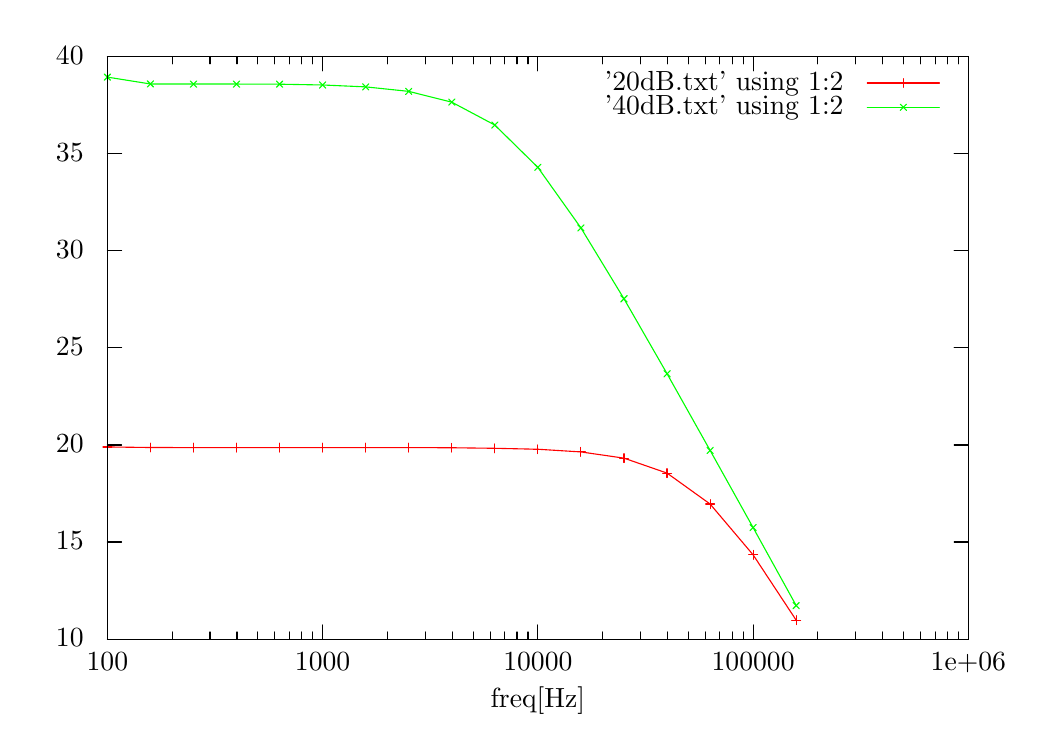
\begin{tikzpicture}[gnuplot]
%% generated with GNUPLOT 4.6p4 (Lua 5.1; terminal rev. 99, script rev. 100)
%% 2016年06月17日 16時24分52秒
\path (0.000,0.000) rectangle (12.500,8.750);
\gpcolor{color=gp lt color border}
\gpsetlinetype{gp lt border}
\gpsetlinewidth{1.00}
\draw[gp path] (1.012,0.985)--(1.192,0.985);
\draw[gp path] (11.947,0.985)--(11.767,0.985);
\node[gp node right] at (0.828,0.985) { 10};
\draw[gp path] (1.012,2.218)--(1.192,2.218);
\draw[gp path] (11.947,2.218)--(11.767,2.218);
\node[gp node right] at (0.828,2.218) { 15};
\draw[gp path] (1.012,3.450)--(1.192,3.450);
\draw[gp path] (11.947,3.450)--(11.767,3.450);
\node[gp node right] at (0.828,3.450) { 20};
\draw[gp path] (1.012,4.683)--(1.192,4.683);
\draw[gp path] (11.947,4.683)--(11.767,4.683);
\node[gp node right] at (0.828,4.683) { 25};
\draw[gp path] (1.012,5.916)--(1.192,5.916);
\draw[gp path] (11.947,5.916)--(11.767,5.916);
\node[gp node right] at (0.828,5.916) { 30};
\draw[gp path] (1.012,7.148)--(1.192,7.148);
\draw[gp path] (11.947,7.148)--(11.767,7.148);
\node[gp node right] at (0.828,7.148) { 35};
\draw[gp path] (1.012,8.381)--(1.192,8.381);
\draw[gp path] (11.947,8.381)--(11.767,8.381);
\node[gp node right] at (0.828,8.381) { 40};
\draw[gp path] (1.012,0.985)--(1.012,1.165);
\draw[gp path] (1.012,8.381)--(1.012,8.201);
\node[gp node center] at (1.012,0.677) { 100};
\draw[gp path] (1.835,0.985)--(1.835,1.075);
\draw[gp path] (1.835,8.381)--(1.835,8.291);
\draw[gp path] (2.316,0.985)--(2.316,1.075);
\draw[gp path] (2.316,8.381)--(2.316,8.291);
\draw[gp path] (2.658,0.985)--(2.658,1.075);
\draw[gp path] (2.658,8.381)--(2.658,8.291);
\draw[gp path] (2.923,0.985)--(2.923,1.075);
\draw[gp path] (2.923,8.381)--(2.923,8.291);
\draw[gp path] (3.139,0.985)--(3.139,1.075);
\draw[gp path] (3.139,8.381)--(3.139,8.291);
\draw[gp path] (3.322,0.985)--(3.322,1.075);
\draw[gp path] (3.322,8.381)--(3.322,8.291);
\draw[gp path] (3.481,0.985)--(3.481,1.075);
\draw[gp path] (3.481,8.381)--(3.481,8.291);
\draw[gp path] (3.621,0.985)--(3.621,1.075);
\draw[gp path] (3.621,8.381)--(3.621,8.291);
\draw[gp path] (3.746,0.985)--(3.746,1.165);
\draw[gp path] (3.746,8.381)--(3.746,8.201);
\node[gp node center] at (3.746,0.677) { 1000};
\draw[gp path] (4.569,0.985)--(4.569,1.075);
\draw[gp path] (4.569,8.381)--(4.569,8.291);
\draw[gp path] (5.050,0.985)--(5.050,1.075);
\draw[gp path] (5.050,8.381)--(5.050,8.291);
\draw[gp path] (5.392,0.985)--(5.392,1.075);
\draw[gp path] (5.392,8.381)--(5.392,8.291);
\draw[gp path] (5.657,0.985)--(5.657,1.075);
\draw[gp path] (5.657,8.381)--(5.657,8.291);
\draw[gp path] (5.873,0.985)--(5.873,1.075);
\draw[gp path] (5.873,8.381)--(5.873,8.291);
\draw[gp path] (6.056,0.985)--(6.056,1.075);
\draw[gp path] (6.056,8.381)--(6.056,8.291);
\draw[gp path] (6.215,0.985)--(6.215,1.075);
\draw[gp path] (6.215,8.381)--(6.215,8.291);
\draw[gp path] (6.354,0.985)--(6.354,1.075);
\draw[gp path] (6.354,8.381)--(6.354,8.291);
\draw[gp path] (6.480,0.985)--(6.480,1.165);
\draw[gp path] (6.480,8.381)--(6.480,8.201);
\node[gp node center] at (6.480,0.677) { 10000};
\draw[gp path] (7.302,0.985)--(7.302,1.075);
\draw[gp path] (7.302,8.381)--(7.302,8.291);
\draw[gp path] (7.784,0.985)--(7.784,1.075);
\draw[gp path] (7.784,8.381)--(7.784,8.291);
\draw[gp path] (8.125,0.985)--(8.125,1.075);
\draw[gp path] (8.125,8.381)--(8.125,8.291);
\draw[gp path] (8.390,0.985)--(8.390,1.075);
\draw[gp path] (8.390,8.381)--(8.390,8.291);
\draw[gp path] (8.607,0.985)--(8.607,1.075);
\draw[gp path] (8.607,8.381)--(8.607,8.291);
\draw[gp path] (8.790,0.985)--(8.790,1.075);
\draw[gp path] (8.790,8.381)--(8.790,8.291);
\draw[gp path] (8.948,0.985)--(8.948,1.075);
\draw[gp path] (8.948,8.381)--(8.948,8.291);
\draw[gp path] (9.088,0.985)--(9.088,1.075);
\draw[gp path] (9.088,8.381)--(9.088,8.291);
\draw[gp path] (9.213,0.985)--(9.213,1.165);
\draw[gp path] (9.213,8.381)--(9.213,8.201);
\node[gp node center] at (9.213,0.677) { 100000};
\draw[gp path] (10.036,0.985)--(10.036,1.075);
\draw[gp path] (10.036,8.381)--(10.036,8.291);
\draw[gp path] (10.518,0.985)--(10.518,1.075);
\draw[gp path] (10.518,8.381)--(10.518,8.291);
\draw[gp path] (10.859,0.985)--(10.859,1.075);
\draw[gp path] (10.859,8.381)--(10.859,8.291);
\draw[gp path] (11.124,0.985)--(11.124,1.075);
\draw[gp path] (11.124,8.381)--(11.124,8.291);
\draw[gp path] (11.341,0.985)--(11.341,1.075);
\draw[gp path] (11.341,8.381)--(11.341,8.291);
\draw[gp path] (11.524,0.985)--(11.524,1.075);
\draw[gp path] (11.524,8.381)--(11.524,8.291);
\draw[gp path] (11.682,0.985)--(11.682,1.075);
\draw[gp path] (11.682,8.381)--(11.682,8.291);
\draw[gp path] (11.822,0.985)--(11.822,1.075);
\draw[gp path] (11.822,8.381)--(11.822,8.291);
\draw[gp path] (11.947,0.985)--(11.947,1.165);
\draw[gp path] (11.947,8.381)--(11.947,8.201);
\node[gp node center] at (11.947,0.677) { 1e+06};
\draw[gp path] (1.012,8.381)--(1.012,0.985)--(11.947,0.985)--(11.947,8.381)--cycle;
\node[gp node center] at (6.479,0.215) {freq[Hz]};
\node[gp node right] at (10.479,8.047) {'20dB.txt' using 1:2};
\gpcolor{color=gp lt color 0}
\gpsetlinetype{gp lt plot 0}
\draw[gp path] (10.663,8.047)--(11.579,8.047);
\draw[gp path] (1.012,3.425)--(1.559,3.418)--(2.106,3.417)--(2.652,3.417)--(3.199,3.417)%
  --(3.746,3.417)--(4.293,3.417)--(4.839,3.417)--(5.386,3.415)--(5.933,3.408)--(6.479,3.396)%
  --(7.026,3.362)--(7.573,3.283)--(8.120,3.093)--(8.667,2.700)--(9.213,2.055)--(9.760,1.225);
\gpsetpointsize{4.00}
\gppoint{gp mark 1}{(1.012,3.425)}
\gppoint{gp mark 1}{(1.559,3.418)}
\gppoint{gp mark 1}{(2.106,3.417)}
\gppoint{gp mark 1}{(2.652,3.417)}
\gppoint{gp mark 1}{(3.199,3.417)}
\gppoint{gp mark 1}{(3.746,3.417)}
\gppoint{gp mark 1}{(4.293,3.417)}
\gppoint{gp mark 1}{(4.839,3.417)}
\gppoint{gp mark 1}{(5.386,3.415)}
\gppoint{gp mark 1}{(5.933,3.408)}
\gppoint{gp mark 1}{(6.479,3.396)}
\gppoint{gp mark 1}{(7.026,3.362)}
\gppoint{gp mark 1}{(7.573,3.283)}
\gppoint{gp mark 1}{(8.120,3.093)}
\gppoint{gp mark 1}{(8.667,2.700)}
\gppoint{gp mark 1}{(9.213,2.055)}
\gppoint{gp mark 1}{(9.760,1.225)}
\gppoint{gp mark 1}{(11.121,8.047)}
\gpcolor{color=gp lt color border}
\node[gp node right] at (10.479,7.739) {'40dB.txt' using 1:2};
\gpcolor{color=gp lt color 1}
\gpsetlinetype{gp lt plot 1}
\draw[gp path] (10.663,7.739)--(11.579,7.739);
\draw[gp path] (1.012,8.122)--(1.559,8.035)--(2.106,8.034)--(2.652,8.034)--(3.199,8.032)%
  --(3.746,8.022)--(4.293,7.998)--(4.839,7.941)--(5.386,7.804)--(5.933,7.513)--(6.479,6.976)%
  --(7.026,6.207)--(7.573,5.307)--(8.120,4.355)--(8.667,3.381)--(9.213,2.401)--(9.760,1.411);
\gppoint{gp mark 2}{(1.012,8.122)}
\gppoint{gp mark 2}{(1.559,8.035)}
\gppoint{gp mark 2}{(2.106,8.034)}
\gppoint{gp mark 2}{(2.652,8.034)}
\gppoint{gp mark 2}{(3.199,8.032)}
\gppoint{gp mark 2}{(3.746,8.022)}
\gppoint{gp mark 2}{(4.293,7.998)}
\gppoint{gp mark 2}{(4.839,7.941)}
\gppoint{gp mark 2}{(5.386,7.804)}
\gppoint{gp mark 2}{(5.933,7.513)}
\gppoint{gp mark 2}{(6.479,6.976)}
\gppoint{gp mark 2}{(7.026,6.207)}
\gppoint{gp mark 2}{(7.573,5.307)}
\gppoint{gp mark 2}{(8.120,4.355)}
\gppoint{gp mark 2}{(8.667,3.381)}
\gppoint{gp mark 2}{(9.213,2.401)}
\gppoint{gp mark 2}{(9.760,1.411)}
\gppoint{gp mark 2}{(11.121,7.739)}
\gpcolor{color=gp lt color border}
\gpsetlinetype{gp lt border}
\draw[gp path] (1.012,8.381)--(1.012,0.985)--(11.947,0.985)--(11.947,8.381)--cycle;
%% coordinates of the plot area
\gpdefrectangularnode{gp plot 1}{\pgfpoint{1.012cm}{0.985cm}}{\pgfpoint{11.947cm}{8.381cm}}
\end{tikzpicture}
%% gnuplot variables
}
        \caption{反転増幅器の振幅特性}
      \end{minipage} &
      %---- 2番目の図 --------------------------
      \begin{minipage}[t]{0.45\hsize}
        \centering
        \scalebox{0.6}{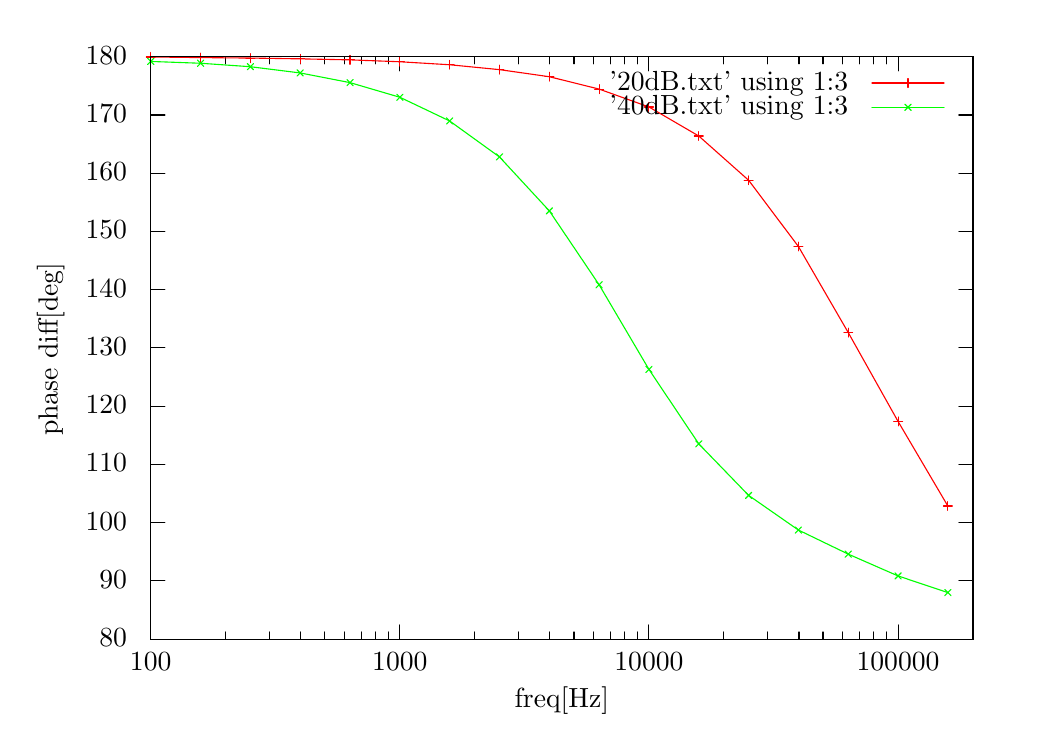
\begin{tikzpicture}[gnuplot]
%% generated with GNUPLOT 4.6p4 (Lua 5.1; terminal rev. 99, script rev. 100)
%% 2016年06月19日 23時01分17秒
\path (0.000,0.000) rectangle (12.500,8.750);
\gpcolor{color=gp lt color border}
\gpsetlinetype{gp lt border}
\gpsetlinewidth{1.00}
\draw[gp path] (1.504,0.985)--(1.684,0.985);
\draw[gp path] (11.947,0.985)--(11.767,0.985);
\node[gp node right] at (1.320,0.985) { 80};
\draw[gp path] (1.504,1.725)--(1.684,1.725);
\draw[gp path] (11.947,1.725)--(11.767,1.725);
\node[gp node right] at (1.320,1.725) { 90};
\draw[gp path] (1.504,2.464)--(1.684,2.464);
\draw[gp path] (11.947,2.464)--(11.767,2.464);
\node[gp node right] at (1.320,2.464) { 100};
\draw[gp path] (1.504,3.204)--(1.684,3.204);
\draw[gp path] (11.947,3.204)--(11.767,3.204);
\node[gp node right] at (1.320,3.204) { 110};
\draw[gp path] (1.504,3.943)--(1.684,3.943);
\draw[gp path] (11.947,3.943)--(11.767,3.943);
\node[gp node right] at (1.320,3.943) { 120};
\draw[gp path] (1.504,4.683)--(1.684,4.683);
\draw[gp path] (11.947,4.683)--(11.767,4.683);
\node[gp node right] at (1.320,4.683) { 130};
\draw[gp path] (1.504,5.423)--(1.684,5.423);
\draw[gp path] (11.947,5.423)--(11.767,5.423);
\node[gp node right] at (1.320,5.423) { 140};
\draw[gp path] (1.504,6.162)--(1.684,6.162);
\draw[gp path] (11.947,6.162)--(11.767,6.162);
\node[gp node right] at (1.320,6.162) { 150};
\draw[gp path] (1.504,6.902)--(1.684,6.902);
\draw[gp path] (11.947,6.902)--(11.767,6.902);
\node[gp node right] at (1.320,6.902) { 160};
\draw[gp path] (1.504,7.641)--(1.684,7.641);
\draw[gp path] (11.947,7.641)--(11.767,7.641);
\node[gp node right] at (1.320,7.641) { 170};
\draw[gp path] (1.504,8.381)--(1.684,8.381);
\draw[gp path] (11.947,8.381)--(11.767,8.381);
\node[gp node right] at (1.320,8.381) { 180};
\draw[gp path] (1.504,0.985)--(1.504,1.165);
\draw[gp path] (1.504,8.381)--(1.504,8.201);
\node[gp node center] at (1.504,0.677) { 100};
\draw[gp path] (2.456,0.985)--(2.456,1.075);
\draw[gp path] (2.456,8.381)--(2.456,8.291);
\draw[gp path] (3.013,0.985)--(3.013,1.075);
\draw[gp path] (3.013,8.381)--(3.013,8.291);
\draw[gp path] (3.409,0.985)--(3.409,1.075);
\draw[gp path] (3.409,8.381)--(3.409,8.291);
\draw[gp path] (3.715,0.985)--(3.715,1.075);
\draw[gp path] (3.715,8.381)--(3.715,8.291);
\draw[gp path] (3.966,0.985)--(3.966,1.075);
\draw[gp path] (3.966,8.381)--(3.966,8.291);
\draw[gp path] (4.178,0.985)--(4.178,1.075);
\draw[gp path] (4.178,8.381)--(4.178,8.291);
\draw[gp path] (4.361,0.985)--(4.361,1.075);
\draw[gp path] (4.361,8.381)--(4.361,8.291);
\draw[gp path] (4.523,0.985)--(4.523,1.075);
\draw[gp path] (4.523,8.381)--(4.523,8.291);
\draw[gp path] (4.668,0.985)--(4.668,1.165);
\draw[gp path] (4.668,8.381)--(4.668,8.201);
\node[gp node center] at (4.668,0.677) { 1000};
\draw[gp path] (5.620,0.985)--(5.620,1.075);
\draw[gp path] (5.620,8.381)--(5.620,8.291);
\draw[gp path] (6.177,0.985)--(6.177,1.075);
\draw[gp path] (6.177,8.381)--(6.177,8.291);
\draw[gp path] (6.572,0.985)--(6.572,1.075);
\draw[gp path] (6.572,8.381)--(6.572,8.291);
\draw[gp path] (6.879,0.985)--(6.879,1.075);
\draw[gp path] (6.879,8.381)--(6.879,8.291);
\draw[gp path] (7.129,0.985)--(7.129,1.075);
\draw[gp path] (7.129,8.381)--(7.129,8.291);
\draw[gp path] (7.341,0.985)--(7.341,1.075);
\draw[gp path] (7.341,8.381)--(7.341,8.291);
\draw[gp path] (7.525,0.985)--(7.525,1.075);
\draw[gp path] (7.525,8.381)--(7.525,8.291);
\draw[gp path] (7.686,0.985)--(7.686,1.075);
\draw[gp path] (7.686,8.381)--(7.686,8.291);
\draw[gp path] (7.831,0.985)--(7.831,1.165);
\draw[gp path] (7.831,8.381)--(7.831,8.201);
\node[gp node center] at (7.831,0.677) { 10000};
\draw[gp path] (8.783,0.985)--(8.783,1.075);
\draw[gp path] (8.783,8.381)--(8.783,8.291);
\draw[gp path] (9.341,0.985)--(9.341,1.075);
\draw[gp path] (9.341,8.381)--(9.341,8.291);
\draw[gp path] (9.736,0.985)--(9.736,1.075);
\draw[gp path] (9.736,8.381)--(9.736,8.291);
\draw[gp path] (10.042,0.985)--(10.042,1.075);
\draw[gp path] (10.042,8.381)--(10.042,8.291);
\draw[gp path] (10.293,0.985)--(10.293,1.075);
\draw[gp path] (10.293,8.381)--(10.293,8.291);
\draw[gp path] (10.505,0.985)--(10.505,1.075);
\draw[gp path] (10.505,8.381)--(10.505,8.291);
\draw[gp path] (10.688,0.985)--(10.688,1.075);
\draw[gp path] (10.688,8.381)--(10.688,8.291);
\draw[gp path] (10.850,0.985)--(10.850,1.075);
\draw[gp path] (10.850,8.381)--(10.850,8.291);
\draw[gp path] (10.995,0.985)--(10.995,1.165);
\draw[gp path] (10.995,8.381)--(10.995,8.201);
\node[gp node center] at (10.995,0.677) { 100000};
\draw[gp path] (11.947,0.985)--(11.947,1.075);
\draw[gp path] (11.947,8.381)--(11.947,8.291);
\draw[gp path] (1.504,8.381)--(1.504,0.985)--(11.947,0.985)--(11.947,8.381)--cycle;
\node[gp node center,rotate=-270] at (0.246,4.683) {phase diff[deg]};
\node[gp node center] at (6.725,0.215) {freq[Hz]};
\node[gp node right] at (10.479,8.047) {'20dB.txt' using 1:3};
\gpcolor{color=gp lt color 0}
\gpsetlinetype{gp lt plot 0}
\draw[gp path] (10.663,8.047)--(11.579,8.047);
\draw[gp path] (1.504,8.378)--(2.137,8.370)--(2.770,8.364)--(3.402,8.354)--(4.035,8.341)%
  --(4.668,8.317)--(5.300,8.279)--(5.933,8.217)--(6.566,8.127)--(7.198,7.970)--(7.831,7.743)%
  --(8.464,7.374)--(9.097,6.812)--(9.729,5.971)--(10.362,4.878)--(10.995,3.749)--(11.627,2.675);
\gpsetpointsize{4.00}
\gppoint{gp mark 1}{(1.504,8.378)}
\gppoint{gp mark 1}{(2.137,8.370)}
\gppoint{gp mark 1}{(2.770,8.364)}
\gppoint{gp mark 1}{(3.402,8.354)}
\gppoint{gp mark 1}{(4.035,8.341)}
\gppoint{gp mark 1}{(4.668,8.317)}
\gppoint{gp mark 1}{(5.300,8.279)}
\gppoint{gp mark 1}{(5.933,8.217)}
\gppoint{gp mark 1}{(6.566,8.127)}
\gppoint{gp mark 1}{(7.198,7.970)}
\gppoint{gp mark 1}{(7.831,7.743)}
\gppoint{gp mark 1}{(8.464,7.374)}
\gppoint{gp mark 1}{(9.097,6.812)}
\gppoint{gp mark 1}{(9.729,5.971)}
\gppoint{gp mark 1}{(10.362,4.878)}
\gppoint{gp mark 1}{(10.995,3.749)}
\gppoint{gp mark 1}{(11.627,2.675)}
\gppoint{gp mark 1}{(11.121,8.047)}
\gpcolor{color=gp lt color border}
\node[gp node right] at (10.479,7.739) {'40dB.txt' using 1:3};
\gpcolor{color=gp lt color 1}
\gpsetlinetype{gp lt plot 1}
\draw[gp path] (10.663,7.739)--(11.579,7.739);
\draw[gp path] (1.504,8.321)--(2.137,8.298)--(2.770,8.254)--(3.402,8.175)--(4.035,8.052)%
  --(4.668,7.866)--(5.300,7.565)--(5.933,7.108)--(6.566,6.423)--(7.198,5.485)--(7.831,4.410)%
  --(8.464,3.464)--(9.097,2.810)--(9.729,2.370)--(10.362,2.064)--(10.995,1.787)--(11.627,1.576);
\gppoint{gp mark 2}{(1.504,8.321)}
\gppoint{gp mark 2}{(2.137,8.298)}
\gppoint{gp mark 2}{(2.770,8.254)}
\gppoint{gp mark 2}{(3.402,8.175)}
\gppoint{gp mark 2}{(4.035,8.052)}
\gppoint{gp mark 2}{(4.668,7.866)}
\gppoint{gp mark 2}{(5.300,7.565)}
\gppoint{gp mark 2}{(5.933,7.108)}
\gppoint{gp mark 2}{(6.566,6.423)}
\gppoint{gp mark 2}{(7.198,5.485)}
\gppoint{gp mark 2}{(7.831,4.410)}
\gppoint{gp mark 2}{(8.464,3.464)}
\gppoint{gp mark 2}{(9.097,2.810)}
\gppoint{gp mark 2}{(9.729,2.370)}
\gppoint{gp mark 2}{(10.362,2.064)}
\gppoint{gp mark 2}{(10.995,1.787)}
\gppoint{gp mark 2}{(11.627,1.576)}
\gppoint{gp mark 2}{(11.121,7.739)}
\gpcolor{color=gp lt color border}
\gpsetlinetype{gp lt border}
\draw[gp path] (1.504,8.381)--(1.504,0.985)--(11.947,0.985)--(11.947,8.381)--cycle;
%% coordinates of the plot area
\gpdefrectangularnode{gp plot 1}{\pgfpoint{1.504cm}{0.985cm}}{\pgfpoint{11.947cm}{8.381cm}}
\end{tikzpicture}
%% gnuplot variables
}
        \caption{反転増幅器の位相特性}
      \end{minipage}
      %---- 図はここまで ----------------------
    \end{tabular}
  \end{figure}
\subsubsection{非反転増幅回路}
反転増幅回路の周波数特性を、図17と図18に示す。	

\begin{figure}[H]
    \begin{tabular}{cc}
      %---- 最初の図 ---------------------------
      \begin{minipage}[t]{0.45\hsize}
        \centering
        \scalebox{0.6}{\input{uninvGain}}
        \caption{非反転増幅器の振幅特性}
      \end{minipage} &
      %---- 2番目の図 --------------------------
      \begin{minipage}[t]{0.45\hsize}
        \centering
        \scalebox{0.6}{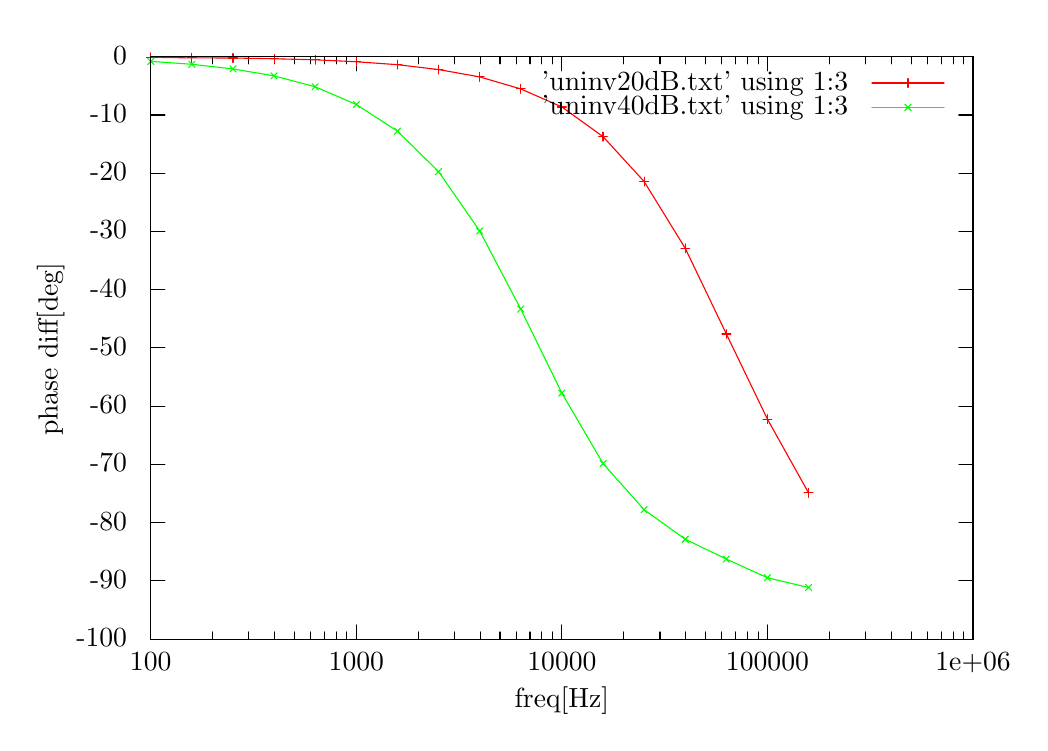
\begin{tikzpicture}[gnuplot]
%% generated with GNUPLOT 4.6p4 (Lua 5.1; terminal rev. 99, script rev. 100)
%% 2016年06月17日 16時38分55秒
\path (0.000,0.000) rectangle (12.500,8.750);
\gpcolor{color=gp lt color border}
\gpsetlinetype{gp lt border}
\gpsetlinewidth{1.00}
\draw[gp path] (1.504,0.985)--(1.684,0.985);
\draw[gp path] (11.947,0.985)--(11.767,0.985);
\node[gp node right] at (1.320,0.985) {-100};
\draw[gp path] (1.504,1.725)--(1.684,1.725);
\draw[gp path] (11.947,1.725)--(11.767,1.725);
\node[gp node right] at (1.320,1.725) {-90};
\draw[gp path] (1.504,2.464)--(1.684,2.464);
\draw[gp path] (11.947,2.464)--(11.767,2.464);
\node[gp node right] at (1.320,2.464) {-80};
\draw[gp path] (1.504,3.204)--(1.684,3.204);
\draw[gp path] (11.947,3.204)--(11.767,3.204);
\node[gp node right] at (1.320,3.204) {-70};
\draw[gp path] (1.504,3.943)--(1.684,3.943);
\draw[gp path] (11.947,3.943)--(11.767,3.943);
\node[gp node right] at (1.320,3.943) {-60};
\draw[gp path] (1.504,4.683)--(1.684,4.683);
\draw[gp path] (11.947,4.683)--(11.767,4.683);
\node[gp node right] at (1.320,4.683) {-50};
\draw[gp path] (1.504,5.423)--(1.684,5.423);
\draw[gp path] (11.947,5.423)--(11.767,5.423);
\node[gp node right] at (1.320,5.423) {-40};
\draw[gp path] (1.504,6.162)--(1.684,6.162);
\draw[gp path] (11.947,6.162)--(11.767,6.162);
\node[gp node right] at (1.320,6.162) {-30};
\draw[gp path] (1.504,6.902)--(1.684,6.902);
\draw[gp path] (11.947,6.902)--(11.767,6.902);
\node[gp node right] at (1.320,6.902) {-20};
\draw[gp path] (1.504,7.641)--(1.684,7.641);
\draw[gp path] (11.947,7.641)--(11.767,7.641);
\node[gp node right] at (1.320,7.641) {-10};
\draw[gp path] (1.504,8.381)--(1.684,8.381);
\draw[gp path] (11.947,8.381)--(11.767,8.381);
\node[gp node right] at (1.320,8.381) { 0};
\draw[gp path] (1.504,0.985)--(1.504,1.165);
\draw[gp path] (1.504,8.381)--(1.504,8.201);
\node[gp node center] at (1.504,0.677) { 100};
\draw[gp path] (2.290,0.985)--(2.290,1.075);
\draw[gp path] (2.290,8.381)--(2.290,8.291);
\draw[gp path] (2.750,0.985)--(2.750,1.075);
\draw[gp path] (2.750,8.381)--(2.750,8.291);
\draw[gp path] (3.076,0.985)--(3.076,1.075);
\draw[gp path] (3.076,8.381)--(3.076,8.291);
\draw[gp path] (3.329,0.985)--(3.329,1.075);
\draw[gp path] (3.329,8.381)--(3.329,8.291);
\draw[gp path] (3.536,0.985)--(3.536,1.075);
\draw[gp path] (3.536,8.381)--(3.536,8.291);
\draw[gp path] (3.710,0.985)--(3.710,1.075);
\draw[gp path] (3.710,8.381)--(3.710,8.291);
\draw[gp path] (3.862,0.985)--(3.862,1.075);
\draw[gp path] (3.862,8.381)--(3.862,8.291);
\draw[gp path] (3.995,0.985)--(3.995,1.075);
\draw[gp path] (3.995,8.381)--(3.995,8.291);
\draw[gp path] (4.115,0.985)--(4.115,1.165);
\draw[gp path] (4.115,8.381)--(4.115,8.201);
\node[gp node center] at (4.115,0.677) { 1000};
\draw[gp path] (4.901,0.985)--(4.901,1.075);
\draw[gp path] (4.901,8.381)--(4.901,8.291);
\draw[gp path] (5.360,0.985)--(5.360,1.075);
\draw[gp path] (5.360,8.381)--(5.360,8.291);
\draw[gp path] (5.687,0.985)--(5.687,1.075);
\draw[gp path] (5.687,8.381)--(5.687,8.291);
\draw[gp path] (5.940,0.985)--(5.940,1.075);
\draw[gp path] (5.940,8.381)--(5.940,8.291);
\draw[gp path] (6.146,0.985)--(6.146,1.075);
\draw[gp path] (6.146,8.381)--(6.146,8.291);
\draw[gp path] (6.321,0.985)--(6.321,1.075);
\draw[gp path] (6.321,8.381)--(6.321,8.291);
\draw[gp path] (6.472,0.985)--(6.472,1.075);
\draw[gp path] (6.472,8.381)--(6.472,8.291);
\draw[gp path] (6.606,0.985)--(6.606,1.075);
\draw[gp path] (6.606,8.381)--(6.606,8.291);
\draw[gp path] (6.726,0.985)--(6.726,1.165);
\draw[gp path] (6.726,8.381)--(6.726,8.201);
\node[gp node center] at (6.726,0.677) { 10000};
\draw[gp path] (7.511,0.985)--(7.511,1.075);
\draw[gp path] (7.511,8.381)--(7.511,8.291);
\draw[gp path] (7.971,0.985)--(7.971,1.075);
\draw[gp path] (7.971,8.381)--(7.971,8.291);
\draw[gp path] (8.297,0.985)--(8.297,1.075);
\draw[gp path] (8.297,8.381)--(8.297,8.291);
\draw[gp path] (8.550,0.985)--(8.550,1.075);
\draw[gp path] (8.550,8.381)--(8.550,8.291);
\draw[gp path] (8.757,0.985)--(8.757,1.075);
\draw[gp path] (8.757,8.381)--(8.757,8.291);
\draw[gp path] (8.932,0.985)--(8.932,1.075);
\draw[gp path] (8.932,8.381)--(8.932,8.291);
\draw[gp path] (9.083,0.985)--(9.083,1.075);
\draw[gp path] (9.083,8.381)--(9.083,8.291);
\draw[gp path] (9.217,0.985)--(9.217,1.075);
\draw[gp path] (9.217,8.381)--(9.217,8.291);
\draw[gp path] (9.336,0.985)--(9.336,1.165);
\draw[gp path] (9.336,8.381)--(9.336,8.201);
\node[gp node center] at (9.336,0.677) { 100000};
\draw[gp path] (10.122,0.985)--(10.122,1.075);
\draw[gp path] (10.122,8.381)--(10.122,8.291);
\draw[gp path] (10.582,0.985)--(10.582,1.075);
\draw[gp path] (10.582,8.381)--(10.582,8.291);
\draw[gp path] (10.908,0.985)--(10.908,1.075);
\draw[gp path] (10.908,8.381)--(10.908,8.291);
\draw[gp path] (11.161,0.985)--(11.161,1.075);
\draw[gp path] (11.161,8.381)--(11.161,8.291);
\draw[gp path] (11.368,0.985)--(11.368,1.075);
\draw[gp path] (11.368,8.381)--(11.368,8.291);
\draw[gp path] (11.543,0.985)--(11.543,1.075);
\draw[gp path] (11.543,8.381)--(11.543,8.291);
\draw[gp path] (11.694,0.985)--(11.694,1.075);
\draw[gp path] (11.694,8.381)--(11.694,8.291);
\draw[gp path] (11.828,0.985)--(11.828,1.075);
\draw[gp path] (11.828,8.381)--(11.828,8.291);
\draw[gp path] (11.947,0.985)--(11.947,1.165);
\draw[gp path] (11.947,8.381)--(11.947,8.201);
\node[gp node center] at (11.947,0.677) { 1e+06};
\draw[gp path] (1.504,8.381)--(1.504,0.985)--(11.947,0.985)--(11.947,8.381)--cycle;
\node[gp node center,rotate=-270] at (0.246,4.683) {phase diff[deg]};
\node[gp node center] at (6.725,0.215) {freq[Hz]};
\node[gp node right] at (10.479,8.047) {'uninv20dB.txt' using 1:3};
\gpcolor{color=gp lt color 0}
\gpsetlinetype{gp lt plot 0}
\draw[gp path] (10.663,8.047)--(11.579,8.047);
\draw[gp path] (1.504,8.374)--(2.026,8.366)--(2.549,8.365)--(3.070,8.355)--(3.592,8.342)%
  --(4.115,8.317)--(4.637,8.280)--(5.159,8.218)--(5.681,8.125)--(6.203,7.972)--(6.725,7.743)%
  --(7.248,7.366)--(7.770,6.796)--(8.292,5.948)--(8.814,4.860)--(9.336,3.778)--(9.858,2.842);
\gpsetpointsize{4.00}
\gppoint{gp mark 1}{(1.504,8.374)}
\gppoint{gp mark 1}{(2.026,8.366)}
\gppoint{gp mark 1}{(2.549,8.365)}
\gppoint{gp mark 1}{(3.070,8.355)}
\gppoint{gp mark 1}{(3.592,8.342)}
\gppoint{gp mark 1}{(4.115,8.317)}
\gppoint{gp mark 1}{(4.637,8.280)}
\gppoint{gp mark 1}{(5.159,8.218)}
\gppoint{gp mark 1}{(5.681,8.125)}
\gppoint{gp mark 1}{(6.203,7.972)}
\gppoint{gp mark 1}{(6.725,7.743)}
\gppoint{gp mark 1}{(7.248,7.366)}
\gppoint{gp mark 1}{(7.770,6.796)}
\gppoint{gp mark 1}{(8.292,5.948)}
\gppoint{gp mark 1}{(8.814,4.860)}
\gppoint{gp mark 1}{(9.336,3.778)}
\gppoint{gp mark 1}{(9.858,2.842)}
\gppoint{gp mark 1}{(11.121,8.047)}
\gpcolor{color=gp lt color border}
\node[gp node right] at (10.479,7.739) {'uninv40dB.txt' using 1:3};
\gpcolor{color=gp lt color 1}
\gpsetlinetype{gp lt plot 1}
\draw[gp path] (10.663,7.739)--(11.579,7.739);
\draw[gp path] (1.504,8.322)--(2.026,8.285)--(2.549,8.226)--(3.070,8.138)--(3.592,7.999)%
  --(4.115,7.774)--(4.637,7.436)--(5.159,6.922)--(5.681,6.169)--(6.203,5.176)--(6.725,4.109)%
  --(7.248,3.214)--(7.770,2.628)--(8.292,2.253)--(8.814,2.001)--(9.336,1.764)--(9.858,1.640);
\gppoint{gp mark 2}{(1.504,8.322)}
\gppoint{gp mark 2}{(2.026,8.285)}
\gppoint{gp mark 2}{(2.549,8.226)}
\gppoint{gp mark 2}{(3.070,8.138)}
\gppoint{gp mark 2}{(3.592,7.999)}
\gppoint{gp mark 2}{(4.115,7.774)}
\gppoint{gp mark 2}{(4.637,7.436)}
\gppoint{gp mark 2}{(5.159,6.922)}
\gppoint{gp mark 2}{(5.681,6.169)}
\gppoint{gp mark 2}{(6.203,5.176)}
\gppoint{gp mark 2}{(6.725,4.109)}
\gppoint{gp mark 2}{(7.248,3.214)}
\gppoint{gp mark 2}{(7.770,2.628)}
\gppoint{gp mark 2}{(8.292,2.253)}
\gppoint{gp mark 2}{(8.814,2.001)}
\gppoint{gp mark 2}{(9.336,1.764)}
\gppoint{gp mark 2}{(9.858,1.640)}
\gppoint{gp mark 2}{(11.121,7.739)}
\gpcolor{color=gp lt color border}
\gpsetlinetype{gp lt border}
\draw[gp path] (1.504,8.381)--(1.504,0.985)--(11.947,0.985)--(11.947,8.381)--cycle;
%% coordinates of the plot area
\gpdefrectangularnode{gp plot 1}{\pgfpoint{1.504cm}{0.985cm}}{\pgfpoint{11.947cm}{8.381cm}}
\end{tikzpicture}
%% gnuplot variables
}
        \caption{非反転増幅器の位相特性}
      \end{minipage}
      %---- 図はここまで ----------------------
    \end{tabular}
  \end{figure}

\subsubsection{反転増幅回路と非反転増幅回路の遮断周波数}
それぞれの回路について、測定結果から得られたおおよその遮断周波数を表11に示す。
\begin{table}[H]
  \begin{center}
    \caption{増幅回路の遮断周波数}
    \begin{tabular}{|l||c|c|c|} \hline
       & \SI{20}{\decibel} & \SI{40}{\decibel} \\ \hline \hline
      反転 & \SI{63}{\kilo\hertz} & \SI{7}{\kilo\hertz}  \\
      非反転 & \SI{63}{\kilo\hertz} & \SI{7}{\kilo\hertz}  \\  
      \hline
    \end{tabular}
  \end{center}
\end{table}
どちらも、この遮断周波数以上の周波数帯では\SI{-20}{\decibel}/decadeの傾きを見せる。
これは、式(1)において、Aが充分小さければ$A_v \simeq \frac{1}{\beta}$、Aが充分大きければ$A_v \simeq A$であることから説明できる。
Aは図1に見るような周波数依存性を持ち、そのため$A(s)\beta$についてどちらが支配的であるかの境界が遮断周波数にあらわれている。
遮断周波数以上の周波数帯で見られる\SI{-20}{\decibel}/decadeの傾きは、図1に見られるようなオペアンプの特性が支配的に表れている結果である。

\subsubsection{微分回路}
微分回路の周波数特性を、図19と図20に示す。	

\begin{figure}[H]
    \begin{tabular}{cc}
      %---- 最初の図 ---------------------------
      \begin{minipage}[t]{0.45\hsize}
        \centering
        \scalebox{0.65}{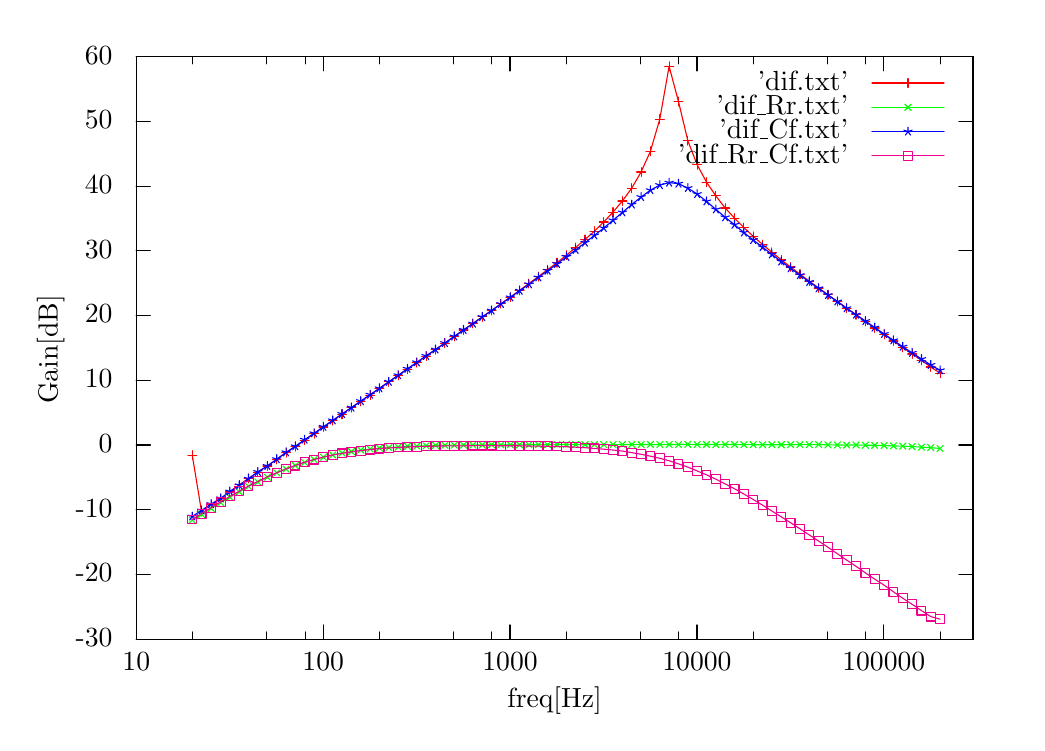
\begin{tikzpicture}[gnuplot]
%% generated with GNUPLOT 4.6p4 (Lua 5.1; terminal rev. 99, script rev. 100)
%% 2016年06月20日 00時00分31秒
\path (0.000,0.000) rectangle (12.500,8.750);
\gpcolor{color=gp lt color border}
\gpsetlinetype{gp lt border}
\gpsetlinewidth{1.00}
\draw[gp path] (1.320,0.985)--(1.500,0.985);
\draw[gp path] (11.947,0.985)--(11.767,0.985);
\node[gp node right] at (1.136,0.985) {-30};
\draw[gp path] (1.320,1.807)--(1.500,1.807);
\draw[gp path] (11.947,1.807)--(11.767,1.807);
\node[gp node right] at (1.136,1.807) {-20};
\draw[gp path] (1.320,2.629)--(1.500,2.629);
\draw[gp path] (11.947,2.629)--(11.767,2.629);
\node[gp node right] at (1.136,2.629) {-10};
\draw[gp path] (1.320,3.450)--(1.500,3.450);
\draw[gp path] (11.947,3.450)--(11.767,3.450);
\node[gp node right] at (1.136,3.450) { 0};
\draw[gp path] (1.320,4.272)--(1.500,4.272);
\draw[gp path] (11.947,4.272)--(11.767,4.272);
\node[gp node right] at (1.136,4.272) { 10};
\draw[gp path] (1.320,5.094)--(1.500,5.094);
\draw[gp path] (11.947,5.094)--(11.767,5.094);
\node[gp node right] at (1.136,5.094) { 20};
\draw[gp path] (1.320,5.916)--(1.500,5.916);
\draw[gp path] (11.947,5.916)--(11.767,5.916);
\node[gp node right] at (1.136,5.916) { 30};
\draw[gp path] (1.320,6.737)--(1.500,6.737);
\draw[gp path] (11.947,6.737)--(11.767,6.737);
\node[gp node right] at (1.136,6.737) { 40};
\draw[gp path] (1.320,7.559)--(1.500,7.559);
\draw[gp path] (11.947,7.559)--(11.767,7.559);
\node[gp node right] at (1.136,7.559) { 50};
\draw[gp path] (1.320,8.381)--(1.500,8.381);
\draw[gp path] (11.947,8.381)--(11.767,8.381);
\node[gp node right] at (1.136,8.381) { 60};
\draw[gp path] (1.320,0.985)--(1.320,1.165);
\draw[gp path] (1.320,8.381)--(1.320,8.201);
\node[gp node center] at (1.320,0.677) { 10};
\draw[gp path] (2.035,0.985)--(2.035,1.075);
\draw[gp path] (2.035,8.381)--(2.035,8.291);
\draw[gp path] (2.979,0.985)--(2.979,1.075);
\draw[gp path] (2.979,8.381)--(2.979,8.291);
\draw[gp path] (3.464,0.985)--(3.464,1.075);
\draw[gp path] (3.464,8.381)--(3.464,8.291);
\draw[gp path] (3.694,0.985)--(3.694,1.165);
\draw[gp path] (3.694,8.381)--(3.694,8.201);
\node[gp node center] at (3.694,0.677) { 100};
\draw[gp path] (4.408,0.985)--(4.408,1.075);
\draw[gp path] (4.408,8.381)--(4.408,8.291);
\draw[gp path] (5.353,0.985)--(5.353,1.075);
\draw[gp path] (5.353,8.381)--(5.353,8.291);
\draw[gp path] (5.837,0.985)--(5.837,1.075);
\draw[gp path] (5.837,8.381)--(5.837,8.291);
\draw[gp path] (6.067,0.985)--(6.067,1.165);
\draw[gp path] (6.067,8.381)--(6.067,8.201);
\node[gp node center] at (6.067,0.677) { 1000};
\draw[gp path] (6.782,0.985)--(6.782,1.075);
\draw[gp path] (6.782,8.381)--(6.782,8.291);
\draw[gp path] (7.726,0.985)--(7.726,1.075);
\draw[gp path] (7.726,8.381)--(7.726,8.291);
\draw[gp path] (8.211,0.985)--(8.211,1.075);
\draw[gp path] (8.211,8.381)--(8.211,8.291);
\draw[gp path] (8.441,0.985)--(8.441,1.165);
\draw[gp path] (8.441,8.381)--(8.441,8.201);
\node[gp node center] at (8.441,0.677) { 10000};
\draw[gp path] (9.155,0.985)--(9.155,1.075);
\draw[gp path] (9.155,8.381)--(9.155,8.291);
\draw[gp path] (10.100,0.985)--(10.100,1.075);
\draw[gp path] (10.100,8.381)--(10.100,8.291);
\draw[gp path] (10.584,0.985)--(10.584,1.075);
\draw[gp path] (10.584,8.381)--(10.584,8.291);
\draw[gp path] (10.814,0.985)--(10.814,1.165);
\draw[gp path] (10.814,8.381)--(10.814,8.201);
\node[gp node center] at (10.814,0.677) { 100000};
\draw[gp path] (11.529,0.985)--(11.529,1.075);
\draw[gp path] (11.529,8.381)--(11.529,8.291);
\draw[gp path] (1.320,8.381)--(1.320,0.985)--(11.947,0.985)--(11.947,8.381)--cycle;
\node[gp node center,rotate=-270] at (0.246,4.683) {Gain[dB]};
\node[gp node center] at (6.633,0.215) {freq[Hz]};
\node[gp node right] at (10.479,8.047) {'dif.txt'};
\gpcolor{color=gp lt color 0}
\gpsetlinetype{gp lt plot 0}
\draw[gp path] (10.663,8.047)--(11.579,8.047);
\draw[gp path] (2.031,3.322)--(2.149,2.605)--(2.271,2.694)--(2.393,2.768)--(2.508,2.856)%
  --(2.628,2.943)--(2.745,3.026)--(2.864,3.105)--(2.985,3.183)--(3.104,3.267)--(3.223,3.354)%
  --(3.340,3.430)--(3.458,3.510)--(3.578,3.594)--(3.696,3.678)--(3.815,3.758)--(3.933,3.841)%
  --(4.052,3.924)--(4.171,4.004)--(4.290,4.083)--(4.408,4.170)--(4.527,4.251)--(4.646,4.333)%
  --(4.764,4.414)--(4.883,4.496)--(5.001,4.577)--(5.120,4.661)--(5.239,4.744)--(5.358,4.828)%
  --(5.476,4.911)--(5.595,4.993)--(5.714,5.077)--(5.832,5.158)--(5.951,5.244)--(6.070,5.328)%
  --(6.188,5.414)--(6.307,5.501)--(6.426,5.589)--(6.544,5.676)--(6.663,5.766)--(6.782,5.861)%
  --(6.900,5.958)--(7.019,6.059)--(7.138,6.166)--(7.257,6.282)--(7.375,6.408)--(7.494,6.549)%
  --(7.613,6.713)--(7.731,6.917)--(7.850,7.181)--(7.969,7.589)--(8.087,8.259)--(8.206,7.812)%
  --(8.325,7.314)--(8.443,7.010)--(8.562,6.789)--(8.681,6.613)--(8.799,6.460)--(8.918,6.331)%
  --(9.037,6.211)--(9.155,6.101)--(9.274,5.996)--(9.393,5.898)--(9.511,5.802)--(9.630,5.711)%
  --(9.749,5.619)--(9.867,5.531)--(9.986,5.444)--(10.105,5.358)--(10.224,5.272)--(10.342,5.188)%
  --(10.461,5.104)--(10.580,5.020)--(10.698,4.936)--(10.817,4.855)--(10.936,4.771)--(11.054,4.689)%
  --(11.173,4.606)--(11.292,4.525)--(11.410,4.441)--(11.529,4.362);
\gpsetpointsize{4.00}
\gppoint{gp mark 1}{(2.031,3.322)}
\gppoint{gp mark 1}{(2.149,2.605)}
\gppoint{gp mark 1}{(2.271,2.694)}
\gppoint{gp mark 1}{(2.393,2.768)}
\gppoint{gp mark 1}{(2.508,2.856)}
\gppoint{gp mark 1}{(2.628,2.943)}
\gppoint{gp mark 1}{(2.745,3.026)}
\gppoint{gp mark 1}{(2.864,3.105)}
\gppoint{gp mark 1}{(2.985,3.183)}
\gppoint{gp mark 1}{(3.104,3.267)}
\gppoint{gp mark 1}{(3.223,3.354)}
\gppoint{gp mark 1}{(3.340,3.430)}
\gppoint{gp mark 1}{(3.458,3.510)}
\gppoint{gp mark 1}{(3.578,3.594)}
\gppoint{gp mark 1}{(3.696,3.678)}
\gppoint{gp mark 1}{(3.815,3.758)}
\gppoint{gp mark 1}{(3.933,3.841)}
\gppoint{gp mark 1}{(4.052,3.924)}
\gppoint{gp mark 1}{(4.171,4.004)}
\gppoint{gp mark 1}{(4.290,4.083)}
\gppoint{gp mark 1}{(4.408,4.170)}
\gppoint{gp mark 1}{(4.527,4.251)}
\gppoint{gp mark 1}{(4.646,4.333)}
\gppoint{gp mark 1}{(4.764,4.414)}
\gppoint{gp mark 1}{(4.883,4.496)}
\gppoint{gp mark 1}{(5.001,4.577)}
\gppoint{gp mark 1}{(5.120,4.661)}
\gppoint{gp mark 1}{(5.239,4.744)}
\gppoint{gp mark 1}{(5.358,4.828)}
\gppoint{gp mark 1}{(5.476,4.911)}
\gppoint{gp mark 1}{(5.595,4.993)}
\gppoint{gp mark 1}{(5.714,5.077)}
\gppoint{gp mark 1}{(5.832,5.158)}
\gppoint{gp mark 1}{(5.951,5.244)}
\gppoint{gp mark 1}{(6.070,5.328)}
\gppoint{gp mark 1}{(6.188,5.414)}
\gppoint{gp mark 1}{(6.307,5.501)}
\gppoint{gp mark 1}{(6.426,5.589)}
\gppoint{gp mark 1}{(6.544,5.676)}
\gppoint{gp mark 1}{(6.663,5.766)}
\gppoint{gp mark 1}{(6.782,5.861)}
\gppoint{gp mark 1}{(6.900,5.958)}
\gppoint{gp mark 1}{(7.019,6.059)}
\gppoint{gp mark 1}{(7.138,6.166)}
\gppoint{gp mark 1}{(7.257,6.282)}
\gppoint{gp mark 1}{(7.375,6.408)}
\gppoint{gp mark 1}{(7.494,6.549)}
\gppoint{gp mark 1}{(7.613,6.713)}
\gppoint{gp mark 1}{(7.731,6.917)}
\gppoint{gp mark 1}{(7.850,7.181)}
\gppoint{gp mark 1}{(7.969,7.589)}
\gppoint{gp mark 1}{(8.087,8.259)}
\gppoint{gp mark 1}{(8.206,7.812)}
\gppoint{gp mark 1}{(8.325,7.314)}
\gppoint{gp mark 1}{(8.443,7.010)}
\gppoint{gp mark 1}{(8.562,6.789)}
\gppoint{gp mark 1}{(8.681,6.613)}
\gppoint{gp mark 1}{(8.799,6.460)}
\gppoint{gp mark 1}{(8.918,6.331)}
\gppoint{gp mark 1}{(9.037,6.211)}
\gppoint{gp mark 1}{(9.155,6.101)}
\gppoint{gp mark 1}{(9.274,5.996)}
\gppoint{gp mark 1}{(9.393,5.898)}
\gppoint{gp mark 1}{(9.511,5.802)}
\gppoint{gp mark 1}{(9.630,5.711)}
\gppoint{gp mark 1}{(9.749,5.619)}
\gppoint{gp mark 1}{(9.867,5.531)}
\gppoint{gp mark 1}{(9.986,5.444)}
\gppoint{gp mark 1}{(10.105,5.358)}
\gppoint{gp mark 1}{(10.224,5.272)}
\gppoint{gp mark 1}{(10.342,5.188)}
\gppoint{gp mark 1}{(10.461,5.104)}
\gppoint{gp mark 1}{(10.580,5.020)}
\gppoint{gp mark 1}{(10.698,4.936)}
\gppoint{gp mark 1}{(10.817,4.855)}
\gppoint{gp mark 1}{(10.936,4.771)}
\gppoint{gp mark 1}{(11.054,4.689)}
\gppoint{gp mark 1}{(11.173,4.606)}
\gppoint{gp mark 1}{(11.292,4.525)}
\gppoint{gp mark 1}{(11.410,4.441)}
\gppoint{gp mark 1}{(11.529,4.362)}
\gppoint{gp mark 1}{(11.121,8.047)}
\gpcolor{color=gp lt color border}
\node[gp node right] at (10.479,7.739) {'dif\_Rr.txt'};
\gpcolor{color=gp lt color 1}
\gpsetlinetype{gp lt plot 1}
\draw[gp path] (10.663,7.739)--(11.579,7.739);
\draw[gp path] (2.031,2.496)--(2.149,2.568)--(2.271,2.645)--(2.393,2.718)--(2.508,2.787)%
  --(2.628,2.855)--(2.745,2.924)--(2.864,2.980)--(2.985,3.041)--(3.104,3.096)--(3.223,3.144)%
  --(3.340,3.189)--(3.458,3.227)--(3.578,3.266)--(3.696,3.295)--(3.815,3.323)--(3.933,3.348)%
  --(4.052,3.366)--(4.171,3.386)--(4.290,3.398)--(4.408,3.411)--(4.527,3.417)--(4.646,3.423)%
  --(4.764,3.433)--(4.883,3.435)--(5.001,3.440)--(5.120,3.446)--(5.239,3.447)--(5.358,3.448)%
  --(5.476,3.448)--(5.595,3.450)--(5.714,3.450)--(5.832,3.454)--(5.951,3.451)--(6.070,3.453)%
  --(6.188,3.452)--(6.307,3.453)--(6.426,3.454)--(6.544,3.454)--(6.663,3.456)--(6.782,3.456)%
  --(6.900,3.455)--(7.019,3.453)--(7.138,3.456)--(7.257,3.455)--(7.375,3.455)--(7.494,3.456)%
  --(7.613,3.457)--(7.731,3.455)--(7.850,3.457)--(7.969,3.456)--(8.087,3.457)--(8.206,3.455)%
  --(8.325,3.458)--(8.443,3.456)--(8.562,3.456)--(8.681,3.455)--(8.799,3.456)--(8.918,3.456)%
  --(9.037,3.454)--(9.155,3.454)--(9.274,3.453)--(9.393,3.454)--(9.511,3.453)--(9.630,3.455)%
  --(9.749,3.456)--(9.867,3.454)--(9.986,3.456)--(10.105,3.452)--(10.224,3.450)--(10.342,3.449)%
  --(10.461,3.450)--(10.580,3.447)--(10.698,3.446)--(10.817,3.443)--(10.936,3.438)--(11.054,3.435)%
  --(11.173,3.430)--(11.292,3.423)--(11.410,3.416)--(11.529,3.406);
\gppoint{gp mark 2}{(2.031,2.496)}
\gppoint{gp mark 2}{(2.149,2.568)}
\gppoint{gp mark 2}{(2.271,2.645)}
\gppoint{gp mark 2}{(2.393,2.718)}
\gppoint{gp mark 2}{(2.508,2.787)}
\gppoint{gp mark 2}{(2.628,2.855)}
\gppoint{gp mark 2}{(2.745,2.924)}
\gppoint{gp mark 2}{(2.864,2.980)}
\gppoint{gp mark 2}{(2.985,3.041)}
\gppoint{gp mark 2}{(3.104,3.096)}
\gppoint{gp mark 2}{(3.223,3.144)}
\gppoint{gp mark 2}{(3.340,3.189)}
\gppoint{gp mark 2}{(3.458,3.227)}
\gppoint{gp mark 2}{(3.578,3.266)}
\gppoint{gp mark 2}{(3.696,3.295)}
\gppoint{gp mark 2}{(3.815,3.323)}
\gppoint{gp mark 2}{(3.933,3.348)}
\gppoint{gp mark 2}{(4.052,3.366)}
\gppoint{gp mark 2}{(4.171,3.386)}
\gppoint{gp mark 2}{(4.290,3.398)}
\gppoint{gp mark 2}{(4.408,3.411)}
\gppoint{gp mark 2}{(4.527,3.417)}
\gppoint{gp mark 2}{(4.646,3.423)}
\gppoint{gp mark 2}{(4.764,3.433)}
\gppoint{gp mark 2}{(4.883,3.435)}
\gppoint{gp mark 2}{(5.001,3.440)}
\gppoint{gp mark 2}{(5.120,3.446)}
\gppoint{gp mark 2}{(5.239,3.447)}
\gppoint{gp mark 2}{(5.358,3.448)}
\gppoint{gp mark 2}{(5.476,3.448)}
\gppoint{gp mark 2}{(5.595,3.450)}
\gppoint{gp mark 2}{(5.714,3.450)}
\gppoint{gp mark 2}{(5.832,3.454)}
\gppoint{gp mark 2}{(5.951,3.451)}
\gppoint{gp mark 2}{(6.070,3.453)}
\gppoint{gp mark 2}{(6.188,3.452)}
\gppoint{gp mark 2}{(6.307,3.453)}
\gppoint{gp mark 2}{(6.426,3.454)}
\gppoint{gp mark 2}{(6.544,3.454)}
\gppoint{gp mark 2}{(6.663,3.456)}
\gppoint{gp mark 2}{(6.782,3.456)}
\gppoint{gp mark 2}{(6.900,3.455)}
\gppoint{gp mark 2}{(7.019,3.453)}
\gppoint{gp mark 2}{(7.138,3.456)}
\gppoint{gp mark 2}{(7.257,3.455)}
\gppoint{gp mark 2}{(7.375,3.455)}
\gppoint{gp mark 2}{(7.494,3.456)}
\gppoint{gp mark 2}{(7.613,3.457)}
\gppoint{gp mark 2}{(7.731,3.455)}
\gppoint{gp mark 2}{(7.850,3.457)}
\gppoint{gp mark 2}{(7.969,3.456)}
\gppoint{gp mark 2}{(8.087,3.457)}
\gppoint{gp mark 2}{(8.206,3.455)}
\gppoint{gp mark 2}{(8.325,3.458)}
\gppoint{gp mark 2}{(8.443,3.456)}
\gppoint{gp mark 2}{(8.562,3.456)}
\gppoint{gp mark 2}{(8.681,3.455)}
\gppoint{gp mark 2}{(8.799,3.456)}
\gppoint{gp mark 2}{(8.918,3.456)}
\gppoint{gp mark 2}{(9.037,3.454)}
\gppoint{gp mark 2}{(9.155,3.454)}
\gppoint{gp mark 2}{(9.274,3.453)}
\gppoint{gp mark 2}{(9.393,3.454)}
\gppoint{gp mark 2}{(9.511,3.453)}
\gppoint{gp mark 2}{(9.630,3.455)}
\gppoint{gp mark 2}{(9.749,3.456)}
\gppoint{gp mark 2}{(9.867,3.454)}
\gppoint{gp mark 2}{(9.986,3.456)}
\gppoint{gp mark 2}{(10.105,3.452)}
\gppoint{gp mark 2}{(10.224,3.450)}
\gppoint{gp mark 2}{(10.342,3.449)}
\gppoint{gp mark 2}{(10.461,3.450)}
\gppoint{gp mark 2}{(10.580,3.447)}
\gppoint{gp mark 2}{(10.698,3.446)}
\gppoint{gp mark 2}{(10.817,3.443)}
\gppoint{gp mark 2}{(10.936,3.438)}
\gppoint{gp mark 2}{(11.054,3.435)}
\gppoint{gp mark 2}{(11.173,3.430)}
\gppoint{gp mark 2}{(11.292,3.423)}
\gppoint{gp mark 2}{(11.410,3.416)}
\gppoint{gp mark 2}{(11.529,3.406)}
\gppoint{gp mark 2}{(11.121,7.739)}
\gpcolor{color=gp lt color border}
\node[gp node right] at (10.479,7.431) {'dif\_Cf.txt'};
\gpcolor{color=gp lt color 2}
\gpsetlinetype{gp lt plot 2}
\draw[gp path] (10.663,7.431)--(11.579,7.431);
\draw[gp path] (2.031,2.542)--(2.149,2.619)--(2.271,2.700)--(2.393,2.773)--(2.508,2.860)%
  --(2.628,2.938)--(2.745,3.022)--(2.864,3.108)--(2.985,3.184)--(3.104,3.270)--(3.223,3.357)%
  --(3.340,3.434)--(3.458,3.517)--(3.578,3.599)--(3.696,3.681)--(3.815,3.763)--(3.933,3.844)%
  --(4.052,3.925)--(4.171,4.008)--(4.290,4.089)--(4.408,4.170)--(4.527,4.253)--(4.646,4.336)%
  --(4.764,4.418)--(4.883,4.500)--(5.001,4.582)--(5.120,4.663)--(5.239,4.745)--(5.358,4.829)%
  --(5.476,4.912)--(5.595,4.992)--(5.714,5.076)--(5.832,5.158)--(5.951,5.241)--(6.070,5.325)%
  --(6.188,5.409)--(6.307,5.491)--(6.426,5.578)--(6.544,5.663)--(6.663,5.749)--(6.782,5.839)%
  --(6.900,5.927)--(7.019,6.019)--(7.138,6.111)--(7.257,6.206)--(7.375,6.304)--(7.494,6.404)%
  --(7.613,6.504)--(7.731,6.599)--(7.850,6.686)--(7.969,6.751)--(8.087,6.782)--(8.206,6.769)%
  --(8.325,6.713)--(8.443,6.637)--(8.562,6.544)--(8.681,6.442)--(8.799,6.342)--(8.918,6.247)%
  --(9.037,6.148)--(9.155,6.053)--(9.274,5.962)--(9.393,5.871)--(9.511,5.780)--(9.630,5.694)%
  --(9.749,5.608)--(9.867,5.521)--(9.986,5.440)--(10.105,5.355)--(10.224,5.273)--(10.342,5.187)%
  --(10.461,5.105)--(10.580,5.024)--(10.698,4.942)--(10.817,4.860)--(10.936,4.780)--(11.054,4.698)%
  --(11.173,4.621)--(11.292,4.542)--(11.410,4.467)--(11.529,4.399);
\gppoint{gp mark 3}{(2.031,2.542)}
\gppoint{gp mark 3}{(2.149,2.619)}
\gppoint{gp mark 3}{(2.271,2.700)}
\gppoint{gp mark 3}{(2.393,2.773)}
\gppoint{gp mark 3}{(2.508,2.860)}
\gppoint{gp mark 3}{(2.628,2.938)}
\gppoint{gp mark 3}{(2.745,3.022)}
\gppoint{gp mark 3}{(2.864,3.108)}
\gppoint{gp mark 3}{(2.985,3.184)}
\gppoint{gp mark 3}{(3.104,3.270)}
\gppoint{gp mark 3}{(3.223,3.357)}
\gppoint{gp mark 3}{(3.340,3.434)}
\gppoint{gp mark 3}{(3.458,3.517)}
\gppoint{gp mark 3}{(3.578,3.599)}
\gppoint{gp mark 3}{(3.696,3.681)}
\gppoint{gp mark 3}{(3.815,3.763)}
\gppoint{gp mark 3}{(3.933,3.844)}
\gppoint{gp mark 3}{(4.052,3.925)}
\gppoint{gp mark 3}{(4.171,4.008)}
\gppoint{gp mark 3}{(4.290,4.089)}
\gppoint{gp mark 3}{(4.408,4.170)}
\gppoint{gp mark 3}{(4.527,4.253)}
\gppoint{gp mark 3}{(4.646,4.336)}
\gppoint{gp mark 3}{(4.764,4.418)}
\gppoint{gp mark 3}{(4.883,4.500)}
\gppoint{gp mark 3}{(5.001,4.582)}
\gppoint{gp mark 3}{(5.120,4.663)}
\gppoint{gp mark 3}{(5.239,4.745)}
\gppoint{gp mark 3}{(5.358,4.829)}
\gppoint{gp mark 3}{(5.476,4.912)}
\gppoint{gp mark 3}{(5.595,4.992)}
\gppoint{gp mark 3}{(5.714,5.076)}
\gppoint{gp mark 3}{(5.832,5.158)}
\gppoint{gp mark 3}{(5.951,5.241)}
\gppoint{gp mark 3}{(6.070,5.325)}
\gppoint{gp mark 3}{(6.188,5.409)}
\gppoint{gp mark 3}{(6.307,5.491)}
\gppoint{gp mark 3}{(6.426,5.578)}
\gppoint{gp mark 3}{(6.544,5.663)}
\gppoint{gp mark 3}{(6.663,5.749)}
\gppoint{gp mark 3}{(6.782,5.839)}
\gppoint{gp mark 3}{(6.900,5.927)}
\gppoint{gp mark 3}{(7.019,6.019)}
\gppoint{gp mark 3}{(7.138,6.111)}
\gppoint{gp mark 3}{(7.257,6.206)}
\gppoint{gp mark 3}{(7.375,6.304)}
\gppoint{gp mark 3}{(7.494,6.404)}
\gppoint{gp mark 3}{(7.613,6.504)}
\gppoint{gp mark 3}{(7.731,6.599)}
\gppoint{gp mark 3}{(7.850,6.686)}
\gppoint{gp mark 3}{(7.969,6.751)}
\gppoint{gp mark 3}{(8.087,6.782)}
\gppoint{gp mark 3}{(8.206,6.769)}
\gppoint{gp mark 3}{(8.325,6.713)}
\gppoint{gp mark 3}{(8.443,6.637)}
\gppoint{gp mark 3}{(8.562,6.544)}
\gppoint{gp mark 3}{(8.681,6.442)}
\gppoint{gp mark 3}{(8.799,6.342)}
\gppoint{gp mark 3}{(8.918,6.247)}
\gppoint{gp mark 3}{(9.037,6.148)}
\gppoint{gp mark 3}{(9.155,6.053)}
\gppoint{gp mark 3}{(9.274,5.962)}
\gppoint{gp mark 3}{(9.393,5.871)}
\gppoint{gp mark 3}{(9.511,5.780)}
\gppoint{gp mark 3}{(9.630,5.694)}
\gppoint{gp mark 3}{(9.749,5.608)}
\gppoint{gp mark 3}{(9.867,5.521)}
\gppoint{gp mark 3}{(9.986,5.440)}
\gppoint{gp mark 3}{(10.105,5.355)}
\gppoint{gp mark 3}{(10.224,5.273)}
\gppoint{gp mark 3}{(10.342,5.187)}
\gppoint{gp mark 3}{(10.461,5.105)}
\gppoint{gp mark 3}{(10.580,5.024)}
\gppoint{gp mark 3}{(10.698,4.942)}
\gppoint{gp mark 3}{(10.817,4.860)}
\gppoint{gp mark 3}{(10.936,4.780)}
\gppoint{gp mark 3}{(11.054,4.698)}
\gppoint{gp mark 3}{(11.173,4.621)}
\gppoint{gp mark 3}{(11.292,4.542)}
\gppoint{gp mark 3}{(11.410,4.467)}
\gppoint{gp mark 3}{(11.529,4.399)}
\gppoint{gp mark 3}{(11.121,7.431)}
\gpcolor{color=gp lt color border}
\node[gp node right] at (10.479,7.123) {'dif\_Rr\_Cf.txt'};
\gpcolor{color=gp lt color 3}
\gpsetlinetype{gp lt plot 3}
\draw[gp path] (10.663,7.123)--(11.579,7.123);
\draw[gp path] (2.031,2.504)--(2.149,2.578)--(2.271,2.654)--(2.393,2.727)--(2.508,2.796)%
  --(2.628,2.862)--(2.745,2.927)--(2.864,2.988)--(2.985,3.044)--(3.104,3.097)--(3.223,3.147)%
  --(3.340,3.189)--(3.458,3.231)--(3.578,3.265)--(3.696,3.296)--(3.815,3.323)--(3.933,3.343)%
  --(4.052,3.363)--(4.171,3.378)--(4.290,3.392)--(4.408,3.404)--(4.527,3.412)--(4.646,3.418)%
  --(4.764,3.424)--(4.883,3.429)--(5.001,3.433)--(5.120,3.435)--(5.239,3.438)--(5.358,3.438)%
  --(5.476,3.439)--(5.595,3.442)--(5.714,3.443)--(5.832,3.442)--(5.951,3.440)--(6.070,3.441)%
  --(6.188,3.440)--(6.307,3.437)--(6.426,3.435)--(6.544,3.434)--(6.663,3.431)--(6.782,3.428)%
  --(6.900,3.422)--(7.019,3.416)--(7.138,3.406)--(7.257,3.397)--(7.375,3.386)--(7.494,3.373)%
  --(7.613,3.353)--(7.731,3.332)--(7.850,3.308)--(7.969,3.281)--(8.087,3.250)--(8.206,3.210)%
  --(8.325,3.169)--(8.443,3.121)--(8.562,3.071)--(8.681,3.016)--(8.799,2.956)--(8.918,2.894)%
  --(9.037,2.827)--(9.155,2.758)--(9.274,2.686)--(9.393,2.611)--(9.511,2.538)--(9.630,2.463)%
  --(9.749,2.386)--(9.867,2.308)--(9.986,2.230)--(10.105,2.151)--(10.224,2.069)--(10.342,1.988)%
  --(10.461,1.909)--(10.580,1.826)--(10.698,1.747)--(10.817,1.670)--(10.936,1.586)--(11.054,1.504)%
  --(11.173,1.427)--(11.292,1.347)--(11.410,1.271)--(11.529,1.238);
\gppoint{gp mark 4}{(2.031,2.504)}
\gppoint{gp mark 4}{(2.149,2.578)}
\gppoint{gp mark 4}{(2.271,2.654)}
\gppoint{gp mark 4}{(2.393,2.727)}
\gppoint{gp mark 4}{(2.508,2.796)}
\gppoint{gp mark 4}{(2.628,2.862)}
\gppoint{gp mark 4}{(2.745,2.927)}
\gppoint{gp mark 4}{(2.864,2.988)}
\gppoint{gp mark 4}{(2.985,3.044)}
\gppoint{gp mark 4}{(3.104,3.097)}
\gppoint{gp mark 4}{(3.223,3.147)}
\gppoint{gp mark 4}{(3.340,3.189)}
\gppoint{gp mark 4}{(3.458,3.231)}
\gppoint{gp mark 4}{(3.578,3.265)}
\gppoint{gp mark 4}{(3.696,3.296)}
\gppoint{gp mark 4}{(3.815,3.323)}
\gppoint{gp mark 4}{(3.933,3.343)}
\gppoint{gp mark 4}{(4.052,3.363)}
\gppoint{gp mark 4}{(4.171,3.378)}
\gppoint{gp mark 4}{(4.290,3.392)}
\gppoint{gp mark 4}{(4.408,3.404)}
\gppoint{gp mark 4}{(4.527,3.412)}
\gppoint{gp mark 4}{(4.646,3.418)}
\gppoint{gp mark 4}{(4.764,3.424)}
\gppoint{gp mark 4}{(4.883,3.429)}
\gppoint{gp mark 4}{(5.001,3.433)}
\gppoint{gp mark 4}{(5.120,3.435)}
\gppoint{gp mark 4}{(5.239,3.438)}
\gppoint{gp mark 4}{(5.358,3.438)}
\gppoint{gp mark 4}{(5.476,3.439)}
\gppoint{gp mark 4}{(5.595,3.442)}
\gppoint{gp mark 4}{(5.714,3.443)}
\gppoint{gp mark 4}{(5.832,3.442)}
\gppoint{gp mark 4}{(5.951,3.440)}
\gppoint{gp mark 4}{(6.070,3.441)}
\gppoint{gp mark 4}{(6.188,3.440)}
\gppoint{gp mark 4}{(6.307,3.437)}
\gppoint{gp mark 4}{(6.426,3.435)}
\gppoint{gp mark 4}{(6.544,3.434)}
\gppoint{gp mark 4}{(6.663,3.431)}
\gppoint{gp mark 4}{(6.782,3.428)}
\gppoint{gp mark 4}{(6.900,3.422)}
\gppoint{gp mark 4}{(7.019,3.416)}
\gppoint{gp mark 4}{(7.138,3.406)}
\gppoint{gp mark 4}{(7.257,3.397)}
\gppoint{gp mark 4}{(7.375,3.386)}
\gppoint{gp mark 4}{(7.494,3.373)}
\gppoint{gp mark 4}{(7.613,3.353)}
\gppoint{gp mark 4}{(7.731,3.332)}
\gppoint{gp mark 4}{(7.850,3.308)}
\gppoint{gp mark 4}{(7.969,3.281)}
\gppoint{gp mark 4}{(8.087,3.250)}
\gppoint{gp mark 4}{(8.206,3.210)}
\gppoint{gp mark 4}{(8.325,3.169)}
\gppoint{gp mark 4}{(8.443,3.121)}
\gppoint{gp mark 4}{(8.562,3.071)}
\gppoint{gp mark 4}{(8.681,3.016)}
\gppoint{gp mark 4}{(8.799,2.956)}
\gppoint{gp mark 4}{(8.918,2.894)}
\gppoint{gp mark 4}{(9.037,2.827)}
\gppoint{gp mark 4}{(9.155,2.758)}
\gppoint{gp mark 4}{(9.274,2.686)}
\gppoint{gp mark 4}{(9.393,2.611)}
\gppoint{gp mark 4}{(9.511,2.538)}
\gppoint{gp mark 4}{(9.630,2.463)}
\gppoint{gp mark 4}{(9.749,2.386)}
\gppoint{gp mark 4}{(9.867,2.308)}
\gppoint{gp mark 4}{(9.986,2.230)}
\gppoint{gp mark 4}{(10.105,2.151)}
\gppoint{gp mark 4}{(10.224,2.069)}
\gppoint{gp mark 4}{(10.342,1.988)}
\gppoint{gp mark 4}{(10.461,1.909)}
\gppoint{gp mark 4}{(10.580,1.826)}
\gppoint{gp mark 4}{(10.698,1.747)}
\gppoint{gp mark 4}{(10.817,1.670)}
\gppoint{gp mark 4}{(10.936,1.586)}
\gppoint{gp mark 4}{(11.054,1.504)}
\gppoint{gp mark 4}{(11.173,1.427)}
\gppoint{gp mark 4}{(11.292,1.347)}
\gppoint{gp mark 4}{(11.410,1.271)}
\gppoint{gp mark 4}{(11.529,1.238)}
\gppoint{gp mark 4}{(11.121,7.123)}
\gpcolor{color=gp lt color border}
\gpsetlinetype{gp lt border}
\draw[gp path] (1.320,8.381)--(1.320,0.985)--(11.947,0.985)--(11.947,8.381)--cycle;
%% coordinates of the plot area
\gpdefrectangularnode{gp plot 1}{\pgfpoint{1.320cm}{0.985cm}}{\pgfpoint{11.947cm}{8.381cm}}
\end{tikzpicture}
}
        \caption{微分器の振幅特性}
      \end{minipage} &
      %---- 2番目の図 --------------------------
      \begin{minipage}[t]{0.45\hsize}
        \centering
        \scalebox{0.65}{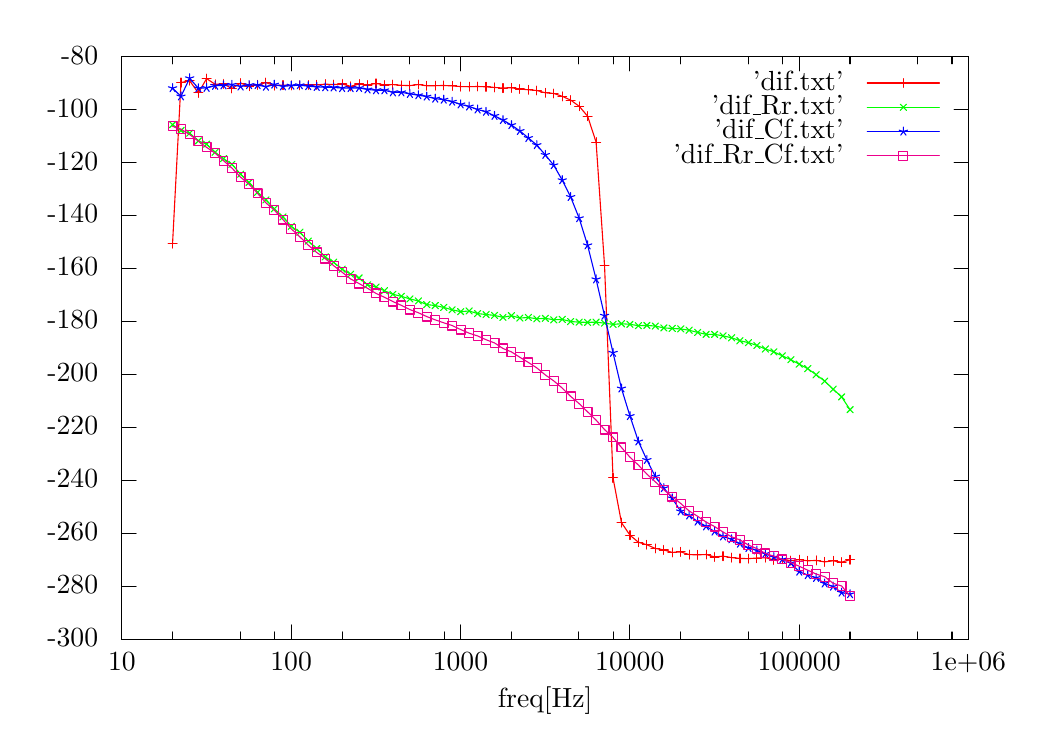
\begin{tikzpicture}[gnuplot]
%% generated with GNUPLOT 4.6p4 (Lua 5.1; terminal rev. 99, script rev. 100)
%% 2016年06月17日 17時25分34秒
\path (0.000,0.000) rectangle (12.500,8.750);
\gpcolor{color=gp lt color border}
\gpsetlinetype{gp lt border}
\gpsetlinewidth{1.00}
\draw[gp path] (1.196,0.985)--(1.376,0.985);
\draw[gp path] (11.947,0.985)--(11.767,0.985);
\node[gp node right] at (1.012,0.985) {-300};
\draw[gp path] (1.196,1.657)--(1.376,1.657);
\draw[gp path] (11.947,1.657)--(11.767,1.657);
\node[gp node right] at (1.012,1.657) {-280};
\draw[gp path] (1.196,2.330)--(1.376,2.330);
\draw[gp path] (11.947,2.330)--(11.767,2.330);
\node[gp node right] at (1.012,2.330) {-260};
\draw[gp path] (1.196,3.002)--(1.376,3.002);
\draw[gp path] (11.947,3.002)--(11.767,3.002);
\node[gp node right] at (1.012,3.002) {-240};
\draw[gp path] (1.196,3.674)--(1.376,3.674);
\draw[gp path] (11.947,3.674)--(11.767,3.674);
\node[gp node right] at (1.012,3.674) {-220};
\draw[gp path] (1.196,4.347)--(1.376,4.347);
\draw[gp path] (11.947,4.347)--(11.767,4.347);
\node[gp node right] at (1.012,4.347) {-200};
\draw[gp path] (1.196,5.019)--(1.376,5.019);
\draw[gp path] (11.947,5.019)--(11.767,5.019);
\node[gp node right] at (1.012,5.019) {-180};
\draw[gp path] (1.196,5.692)--(1.376,5.692);
\draw[gp path] (11.947,5.692)--(11.767,5.692);
\node[gp node right] at (1.012,5.692) {-160};
\draw[gp path] (1.196,6.364)--(1.376,6.364);
\draw[gp path] (11.947,6.364)--(11.767,6.364);
\node[gp node right] at (1.012,6.364) {-140};
\draw[gp path] (1.196,7.036)--(1.376,7.036);
\draw[gp path] (11.947,7.036)--(11.767,7.036);
\node[gp node right] at (1.012,7.036) {-120};
\draw[gp path] (1.196,7.709)--(1.376,7.709);
\draw[gp path] (11.947,7.709)--(11.767,7.709);
\node[gp node right] at (1.012,7.709) {-100};
\draw[gp path] (1.196,8.381)--(1.376,8.381);
\draw[gp path] (11.947,8.381)--(11.767,8.381);
\node[gp node right] at (1.012,8.381) {-80};
\draw[gp path] (1.196,0.985)--(1.196,1.165);
\draw[gp path] (1.196,8.381)--(1.196,8.201);
\node[gp node center] at (1.196,0.677) { 10};
\draw[gp path] (1.843,0.985)--(1.843,1.075);
\draw[gp path] (1.843,8.381)--(1.843,8.291);
\draw[gp path] (2.699,0.985)--(2.699,1.075);
\draw[gp path] (2.699,8.381)--(2.699,8.291);
\draw[gp path] (3.138,0.985)--(3.138,1.075);
\draw[gp path] (3.138,8.381)--(3.138,8.291);
\draw[gp path] (3.346,0.985)--(3.346,1.165);
\draw[gp path] (3.346,8.381)--(3.346,8.201);
\node[gp node center] at (3.346,0.677) { 100};
\draw[gp path] (3.993,0.985)--(3.993,1.075);
\draw[gp path] (3.993,8.381)--(3.993,8.291);
\draw[gp path] (4.849,0.985)--(4.849,1.075);
\draw[gp path] (4.849,8.381)--(4.849,8.291);
\draw[gp path] (5.288,0.985)--(5.288,1.075);
\draw[gp path] (5.288,8.381)--(5.288,8.291);
\draw[gp path] (5.496,0.985)--(5.496,1.165);
\draw[gp path] (5.496,8.381)--(5.496,8.201);
\node[gp node center] at (5.496,0.677) { 1000};
\draw[gp path] (6.144,0.985)--(6.144,1.075);
\draw[gp path] (6.144,8.381)--(6.144,8.291);
\draw[gp path] (6.999,0.985)--(6.999,1.075);
\draw[gp path] (6.999,8.381)--(6.999,8.291);
\draw[gp path] (7.438,0.985)--(7.438,1.075);
\draw[gp path] (7.438,8.381)--(7.438,8.291);
\draw[gp path] (7.647,0.985)--(7.647,1.165);
\draw[gp path] (7.647,8.381)--(7.647,8.201);
\node[gp node center] at (7.647,0.677) { 10000};
\draw[gp path] (8.294,0.985)--(8.294,1.075);
\draw[gp path] (8.294,8.381)--(8.294,8.291);
\draw[gp path] (9.150,0.985)--(9.150,1.075);
\draw[gp path] (9.150,8.381)--(9.150,8.291);
\draw[gp path] (9.588,0.985)--(9.588,1.075);
\draw[gp path] (9.588,8.381)--(9.588,8.291);
\draw[gp path] (9.797,0.985)--(9.797,1.165);
\draw[gp path] (9.797,8.381)--(9.797,8.201);
\node[gp node center] at (9.797,0.677) { 100000};
\draw[gp path] (10.444,0.985)--(10.444,1.075);
\draw[gp path] (10.444,8.381)--(10.444,8.291);
\draw[gp path] (11.300,0.985)--(11.300,1.075);
\draw[gp path] (11.300,8.381)--(11.300,8.291);
\draw[gp path] (11.739,0.985)--(11.739,1.075);
\draw[gp path] (11.739,8.381)--(11.739,8.291);
\draw[gp path] (11.947,0.985)--(11.947,1.165);
\draw[gp path] (11.947,8.381)--(11.947,8.201);
\node[gp node center] at (11.947,0.677) { 1e+06};
\draw[gp path] (1.196,8.381)--(1.196,0.985)--(11.947,0.985)--(11.947,8.381)--cycle;
\node[gp node center] at (6.571,0.215) {freq[Hz]};
\node[gp node right] at (10.479,8.047) {'dif.txt'};
\gpcolor{color=gp lt color 0}
\gpsetlinetype{gp lt plot 0}
\draw[gp path] (10.663,8.047)--(11.579,8.047);
\draw[gp path] (1.840,6.008)--(1.947,8.053)--(2.057,8.076)--(2.168,7.921)--(2.272,8.103)%
  --(2.381,8.031)--(2.487,8.035)--(2.594,7.978)--(2.704,8.046)--(2.812,8.008)--(2.920,8.023)%
  --(3.026,8.052)--(3.132,8.014)--(3.242,8.021)--(3.348,8.017)--(3.456,8.018)--(3.563,8.022)%
  --(3.671,8.023)--(3.779,8.033)--(3.886,8.027)--(3.994,8.035)--(4.101,8.005)--(4.209,8.034)%
  --(4.316,8.022)--(4.424,8.042)--(4.531,8.022)--(4.638,8.027)--(4.746,8.018)--(4.854,8.014)%
  --(4.961,8.028)--(5.068,8.012)--(5.176,8.013)--(5.284,8.016)--(5.391,8.010)--(5.499,8.002)%
  --(5.606,8.000)--(5.714,8.003)--(5.821,7.999)--(5.929,7.991)--(6.036,7.983)--(6.144,7.986)%
  --(6.251,7.971)--(6.359,7.961)--(6.466,7.952)--(6.574,7.923)--(6.681,7.914)--(6.789,7.878)%
  --(6.896,7.830)--(7.004,7.752)--(7.111,7.626)--(7.219,7.296)--(7.326,5.731)--(7.434,3.032)%
  --(7.541,2.464)--(7.649,2.305)--(7.756,2.215)--(7.864,2.183)--(7.971,2.136)--(8.079,2.117)%
  --(8.186,2.086)--(8.294,2.092)--(8.401,2.058)--(8.509,2.055)--(8.616,2.059)--(8.724,2.028)%
  --(8.831,2.038)--(8.939,2.020)--(9.046,2.009)--(9.154,2.007)--(9.261,2.014)--(9.369,2.019)%
  --(9.476,1.991)--(9.584,1.999)--(9.692,1.982)--(9.799,1.993)--(9.907,1.979)--(10.014,1.984)%
  --(10.122,1.965)--(10.229,1.979)--(10.337,1.962)--(10.444,1.993);
\gpsetpointsize{4.00}
\gppoint{gp mark 1}{(1.840,6.008)}
\gppoint{gp mark 1}{(1.947,8.053)}
\gppoint{gp mark 1}{(2.057,8.076)}
\gppoint{gp mark 1}{(2.168,7.921)}
\gppoint{gp mark 1}{(2.272,8.103)}
\gppoint{gp mark 1}{(2.381,8.031)}
\gppoint{gp mark 1}{(2.487,8.035)}
\gppoint{gp mark 1}{(2.594,7.978)}
\gppoint{gp mark 1}{(2.704,8.046)}
\gppoint{gp mark 1}{(2.812,8.008)}
\gppoint{gp mark 1}{(2.920,8.023)}
\gppoint{gp mark 1}{(3.026,8.052)}
\gppoint{gp mark 1}{(3.132,8.014)}
\gppoint{gp mark 1}{(3.242,8.021)}
\gppoint{gp mark 1}{(3.348,8.017)}
\gppoint{gp mark 1}{(3.456,8.018)}
\gppoint{gp mark 1}{(3.563,8.022)}
\gppoint{gp mark 1}{(3.671,8.023)}
\gppoint{gp mark 1}{(3.779,8.033)}
\gppoint{gp mark 1}{(3.886,8.027)}
\gppoint{gp mark 1}{(3.994,8.035)}
\gppoint{gp mark 1}{(4.101,8.005)}
\gppoint{gp mark 1}{(4.209,8.034)}
\gppoint{gp mark 1}{(4.316,8.022)}
\gppoint{gp mark 1}{(4.424,8.042)}
\gppoint{gp mark 1}{(4.531,8.022)}
\gppoint{gp mark 1}{(4.638,8.027)}
\gppoint{gp mark 1}{(4.746,8.018)}
\gppoint{gp mark 1}{(4.854,8.014)}
\gppoint{gp mark 1}{(4.961,8.028)}
\gppoint{gp mark 1}{(5.068,8.012)}
\gppoint{gp mark 1}{(5.176,8.013)}
\gppoint{gp mark 1}{(5.284,8.016)}
\gppoint{gp mark 1}{(5.391,8.010)}
\gppoint{gp mark 1}{(5.499,8.002)}
\gppoint{gp mark 1}{(5.606,8.000)}
\gppoint{gp mark 1}{(5.714,8.003)}
\gppoint{gp mark 1}{(5.821,7.999)}
\gppoint{gp mark 1}{(5.929,7.991)}
\gppoint{gp mark 1}{(6.036,7.983)}
\gppoint{gp mark 1}{(6.144,7.986)}
\gppoint{gp mark 1}{(6.251,7.971)}
\gppoint{gp mark 1}{(6.359,7.961)}
\gppoint{gp mark 1}{(6.466,7.952)}
\gppoint{gp mark 1}{(6.574,7.923)}
\gppoint{gp mark 1}{(6.681,7.914)}
\gppoint{gp mark 1}{(6.789,7.878)}
\gppoint{gp mark 1}{(6.896,7.830)}
\gppoint{gp mark 1}{(7.004,7.752)}
\gppoint{gp mark 1}{(7.111,7.626)}
\gppoint{gp mark 1}{(7.219,7.296)}
\gppoint{gp mark 1}{(7.326,5.731)}
\gppoint{gp mark 1}{(7.434,3.032)}
\gppoint{gp mark 1}{(7.541,2.464)}
\gppoint{gp mark 1}{(7.649,2.305)}
\gppoint{gp mark 1}{(7.756,2.215)}
\gppoint{gp mark 1}{(7.864,2.183)}
\gppoint{gp mark 1}{(7.971,2.136)}
\gppoint{gp mark 1}{(8.079,2.117)}
\gppoint{gp mark 1}{(8.186,2.086)}
\gppoint{gp mark 1}{(8.294,2.092)}
\gppoint{gp mark 1}{(8.401,2.058)}
\gppoint{gp mark 1}{(8.509,2.055)}
\gppoint{gp mark 1}{(8.616,2.059)}
\gppoint{gp mark 1}{(8.724,2.028)}
\gppoint{gp mark 1}{(8.831,2.038)}
\gppoint{gp mark 1}{(8.939,2.020)}
\gppoint{gp mark 1}{(9.046,2.009)}
\gppoint{gp mark 1}{(9.154,2.007)}
\gppoint{gp mark 1}{(9.261,2.014)}
\gppoint{gp mark 1}{(9.369,2.019)}
\gppoint{gp mark 1}{(9.476,1.991)}
\gppoint{gp mark 1}{(9.584,1.999)}
\gppoint{gp mark 1}{(9.692,1.982)}
\gppoint{gp mark 1}{(9.799,1.993)}
\gppoint{gp mark 1}{(9.907,1.979)}
\gppoint{gp mark 1}{(10.014,1.984)}
\gppoint{gp mark 1}{(10.122,1.965)}
\gppoint{gp mark 1}{(10.229,1.979)}
\gppoint{gp mark 1}{(10.337,1.962)}
\gppoint{gp mark 1}{(10.444,1.993)}
\gppoint{gp mark 1}{(11.121,8.047)}
\gpcolor{color=gp lt color border}
\node[gp node right] at (10.479,7.739) {'dif\_Rr.txt'};
\gpcolor{color=gp lt color 1}
\gpsetlinetype{gp lt plot 1}
\draw[gp path] (10.663,7.739)--(11.579,7.739);
\draw[gp path] (1.840,7.518)--(1.947,7.444)--(2.057,7.410)--(2.168,7.312)--(2.272,7.270)%
  --(2.381,7.168)--(2.487,7.087)--(2.594,7.015)--(2.704,6.889)--(2.812,6.785)--(2.920,6.660)%
  --(3.026,6.563)--(3.132,6.449)--(3.242,6.347)--(3.348,6.226)--(3.456,6.152)--(3.563,6.040)%
  --(3.671,5.945)--(3.779,5.838)--(3.886,5.771)--(3.994,5.682)--(4.101,5.619)--(4.209,5.572)%
  --(4.316,5.484)--(4.424,5.456)--(4.531,5.409)--(4.638,5.364)--(4.746,5.338)--(4.854,5.305)%
  --(4.961,5.279)--(5.068,5.233)--(5.176,5.221)--(5.284,5.197)--(5.391,5.167)--(5.499,5.143)%
  --(5.606,5.152)--(5.714,5.119)--(5.821,5.107)--(5.929,5.096)--(6.036,5.071)--(6.144,5.092)%
  --(6.251,5.062)--(6.359,5.070)--(6.466,5.052)--(6.574,5.059)--(6.681,5.040)--(6.789,5.045)%
  --(6.896,5.018)--(7.004,5.010)--(7.111,5.007)--(7.219,5.010)--(7.326,4.997)--(7.434,4.982)%
  --(7.541,4.990)--(7.649,4.983)--(7.756,4.965)--(7.864,4.969)--(7.971,4.960)--(8.079,4.937)%
  --(8.186,4.930)--(8.294,4.924)--(8.401,4.907)--(8.509,4.880)--(8.616,4.855)--(8.724,4.855)%
  --(8.831,4.836)--(8.939,4.812)--(9.046,4.774)--(9.154,4.750)--(9.261,4.714)--(9.369,4.669)%
  --(9.476,4.633)--(9.584,4.582)--(9.692,4.533)--(9.799,4.476)--(9.907,4.419)--(10.014,4.342)%
  --(10.122,4.261)--(10.229,4.159)--(10.337,4.061)--(10.444,3.898);
\gppoint{gp mark 2}{(1.840,7.518)}
\gppoint{gp mark 2}{(1.947,7.444)}
\gppoint{gp mark 2}{(2.057,7.410)}
\gppoint{gp mark 2}{(2.168,7.312)}
\gppoint{gp mark 2}{(2.272,7.270)}
\gppoint{gp mark 2}{(2.381,7.168)}
\gppoint{gp mark 2}{(2.487,7.087)}
\gppoint{gp mark 2}{(2.594,7.015)}
\gppoint{gp mark 2}{(2.704,6.889)}
\gppoint{gp mark 2}{(2.812,6.785)}
\gppoint{gp mark 2}{(2.920,6.660)}
\gppoint{gp mark 2}{(3.026,6.563)}
\gppoint{gp mark 2}{(3.132,6.449)}
\gppoint{gp mark 2}{(3.242,6.347)}
\gppoint{gp mark 2}{(3.348,6.226)}
\gppoint{gp mark 2}{(3.456,6.152)}
\gppoint{gp mark 2}{(3.563,6.040)}
\gppoint{gp mark 2}{(3.671,5.945)}
\gppoint{gp mark 2}{(3.779,5.838)}
\gppoint{gp mark 2}{(3.886,5.771)}
\gppoint{gp mark 2}{(3.994,5.682)}
\gppoint{gp mark 2}{(4.101,5.619)}
\gppoint{gp mark 2}{(4.209,5.572)}
\gppoint{gp mark 2}{(4.316,5.484)}
\gppoint{gp mark 2}{(4.424,5.456)}
\gppoint{gp mark 2}{(4.531,5.409)}
\gppoint{gp mark 2}{(4.638,5.364)}
\gppoint{gp mark 2}{(4.746,5.338)}
\gppoint{gp mark 2}{(4.854,5.305)}
\gppoint{gp mark 2}{(4.961,5.279)}
\gppoint{gp mark 2}{(5.068,5.233)}
\gppoint{gp mark 2}{(5.176,5.221)}
\gppoint{gp mark 2}{(5.284,5.197)}
\gppoint{gp mark 2}{(5.391,5.167)}
\gppoint{gp mark 2}{(5.499,5.143)}
\gppoint{gp mark 2}{(5.606,5.152)}
\gppoint{gp mark 2}{(5.714,5.119)}
\gppoint{gp mark 2}{(5.821,5.107)}
\gppoint{gp mark 2}{(5.929,5.096)}
\gppoint{gp mark 2}{(6.036,5.071)}
\gppoint{gp mark 2}{(6.144,5.092)}
\gppoint{gp mark 2}{(6.251,5.062)}
\gppoint{gp mark 2}{(6.359,5.070)}
\gppoint{gp mark 2}{(6.466,5.052)}
\gppoint{gp mark 2}{(6.574,5.059)}
\gppoint{gp mark 2}{(6.681,5.040)}
\gppoint{gp mark 2}{(6.789,5.045)}
\gppoint{gp mark 2}{(6.896,5.018)}
\gppoint{gp mark 2}{(7.004,5.010)}
\gppoint{gp mark 2}{(7.111,5.007)}
\gppoint{gp mark 2}{(7.219,5.010)}
\gppoint{gp mark 2}{(7.326,4.997)}
\gppoint{gp mark 2}{(7.434,4.982)}
\gppoint{gp mark 2}{(7.541,4.990)}
\gppoint{gp mark 2}{(7.649,4.983)}
\gppoint{gp mark 2}{(7.756,4.965)}
\gppoint{gp mark 2}{(7.864,4.969)}
\gppoint{gp mark 2}{(7.971,4.960)}
\gppoint{gp mark 2}{(8.079,4.937)}
\gppoint{gp mark 2}{(8.186,4.930)}
\gppoint{gp mark 2}{(8.294,4.924)}
\gppoint{gp mark 2}{(8.401,4.907)}
\gppoint{gp mark 2}{(8.509,4.880)}
\gppoint{gp mark 2}{(8.616,4.855)}
\gppoint{gp mark 2}{(8.724,4.855)}
\gppoint{gp mark 2}{(8.831,4.836)}
\gppoint{gp mark 2}{(8.939,4.812)}
\gppoint{gp mark 2}{(9.046,4.774)}
\gppoint{gp mark 2}{(9.154,4.750)}
\gppoint{gp mark 2}{(9.261,4.714)}
\gppoint{gp mark 2}{(9.369,4.669)}
\gppoint{gp mark 2}{(9.476,4.633)}
\gppoint{gp mark 2}{(9.584,4.582)}
\gppoint{gp mark 2}{(9.692,4.533)}
\gppoint{gp mark 2}{(9.799,4.476)}
\gppoint{gp mark 2}{(9.907,4.419)}
\gppoint{gp mark 2}{(10.014,4.342)}
\gppoint{gp mark 2}{(10.122,4.261)}
\gppoint{gp mark 2}{(10.229,4.159)}
\gppoint{gp mark 2}{(10.337,4.061)}
\gppoint{gp mark 2}{(10.444,3.898)}
\gppoint{gp mark 2}{(11.121,7.739)}
\gpcolor{color=gp lt color border}
\node[gp node right] at (10.479,7.431) {'dif\_Cf.txt'};
\gpcolor{color=gp lt color 2}
\gpsetlinetype{gp lt plot 2}
\draw[gp path] (10.663,7.431)--(11.579,7.431);
\draw[gp path] (1.840,7.982)--(1.947,7.877)--(2.057,8.108)--(2.168,7.980)--(2.272,7.986)%
  --(2.381,8.012)--(2.487,8.017)--(2.594,8.025)--(2.704,8.003)--(2.812,8.021)--(2.920,8.020)%
  --(3.026,8.000)--(3.132,8.027)--(3.242,8.004)--(3.348,8.014)--(3.456,8.019)--(3.563,8.007)%
  --(3.671,7.997)--(3.779,7.993)--(3.886,7.991)--(3.994,7.983)--(4.101,7.983)--(4.209,7.984)%
  --(4.316,7.965)--(4.424,7.955)--(4.531,7.955)--(4.638,7.929)--(4.746,7.929)--(4.854,7.909)%
  --(4.961,7.892)--(5.068,7.875)--(5.176,7.849)--(5.284,7.835)--(5.391,7.810)--(5.499,7.776)%
  --(5.606,7.749)--(5.714,7.711)--(5.821,7.682)--(5.929,7.630)--(6.036,7.577)--(6.144,7.513)%
  --(6.251,7.438)--(6.359,7.349)--(6.466,7.259)--(6.574,7.134)--(6.681,7.003)--(6.789,6.813)%
  --(6.896,6.600)--(7.004,6.330)--(7.111,5.986)--(7.219,5.554)--(7.326,5.092)--(7.434,4.621)%
  --(7.541,4.168)--(7.649,3.818)--(7.756,3.495)--(7.864,3.260)--(7.971,3.049)--(8.079,2.902)%
  --(8.186,2.773)--(8.294,2.607)--(8.401,2.555)--(8.509,2.478)--(8.616,2.417)--(8.724,2.351)%
  --(8.831,2.288)--(8.939,2.253)--(9.046,2.197)--(9.154,2.142)--(9.261,2.111)--(9.369,2.068)%
  --(9.476,2.026)--(9.584,1.998)--(9.692,1.951)--(9.799,1.841)--(9.907,1.797)--(10.014,1.763)%
  --(10.122,1.691)--(10.229,1.652)--(10.337,1.575)--(10.444,1.555);
\gppoint{gp mark 3}{(1.840,7.982)}
\gppoint{gp mark 3}{(1.947,7.877)}
\gppoint{gp mark 3}{(2.057,8.108)}
\gppoint{gp mark 3}{(2.168,7.980)}
\gppoint{gp mark 3}{(2.272,7.986)}
\gppoint{gp mark 3}{(2.381,8.012)}
\gppoint{gp mark 3}{(2.487,8.017)}
\gppoint{gp mark 3}{(2.594,8.025)}
\gppoint{gp mark 3}{(2.704,8.003)}
\gppoint{gp mark 3}{(2.812,8.021)}
\gppoint{gp mark 3}{(2.920,8.020)}
\gppoint{gp mark 3}{(3.026,8.000)}
\gppoint{gp mark 3}{(3.132,8.027)}
\gppoint{gp mark 3}{(3.242,8.004)}
\gppoint{gp mark 3}{(3.348,8.014)}
\gppoint{gp mark 3}{(3.456,8.019)}
\gppoint{gp mark 3}{(3.563,8.007)}
\gppoint{gp mark 3}{(3.671,7.997)}
\gppoint{gp mark 3}{(3.779,7.993)}
\gppoint{gp mark 3}{(3.886,7.991)}
\gppoint{gp mark 3}{(3.994,7.983)}
\gppoint{gp mark 3}{(4.101,7.983)}
\gppoint{gp mark 3}{(4.209,7.984)}
\gppoint{gp mark 3}{(4.316,7.965)}
\gppoint{gp mark 3}{(4.424,7.955)}
\gppoint{gp mark 3}{(4.531,7.955)}
\gppoint{gp mark 3}{(4.638,7.929)}
\gppoint{gp mark 3}{(4.746,7.929)}
\gppoint{gp mark 3}{(4.854,7.909)}
\gppoint{gp mark 3}{(4.961,7.892)}
\gppoint{gp mark 3}{(5.068,7.875)}
\gppoint{gp mark 3}{(5.176,7.849)}
\gppoint{gp mark 3}{(5.284,7.835)}
\gppoint{gp mark 3}{(5.391,7.810)}
\gppoint{gp mark 3}{(5.499,7.776)}
\gppoint{gp mark 3}{(5.606,7.749)}
\gppoint{gp mark 3}{(5.714,7.711)}
\gppoint{gp mark 3}{(5.821,7.682)}
\gppoint{gp mark 3}{(5.929,7.630)}
\gppoint{gp mark 3}{(6.036,7.577)}
\gppoint{gp mark 3}{(6.144,7.513)}
\gppoint{gp mark 3}{(6.251,7.438)}
\gppoint{gp mark 3}{(6.359,7.349)}
\gppoint{gp mark 3}{(6.466,7.259)}
\gppoint{gp mark 3}{(6.574,7.134)}
\gppoint{gp mark 3}{(6.681,7.003)}
\gppoint{gp mark 3}{(6.789,6.813)}
\gppoint{gp mark 3}{(6.896,6.600)}
\gppoint{gp mark 3}{(7.004,6.330)}
\gppoint{gp mark 3}{(7.111,5.986)}
\gppoint{gp mark 3}{(7.219,5.554)}
\gppoint{gp mark 3}{(7.326,5.092)}
\gppoint{gp mark 3}{(7.434,4.621)}
\gppoint{gp mark 3}{(7.541,4.168)}
\gppoint{gp mark 3}{(7.649,3.818)}
\gppoint{gp mark 3}{(7.756,3.495)}
\gppoint{gp mark 3}{(7.864,3.260)}
\gppoint{gp mark 3}{(7.971,3.049)}
\gppoint{gp mark 3}{(8.079,2.902)}
\gppoint{gp mark 3}{(8.186,2.773)}
\gppoint{gp mark 3}{(8.294,2.607)}
\gppoint{gp mark 3}{(8.401,2.555)}
\gppoint{gp mark 3}{(8.509,2.478)}
\gppoint{gp mark 3}{(8.616,2.417)}
\gppoint{gp mark 3}{(8.724,2.351)}
\gppoint{gp mark 3}{(8.831,2.288)}
\gppoint{gp mark 3}{(8.939,2.253)}
\gppoint{gp mark 3}{(9.046,2.197)}
\gppoint{gp mark 3}{(9.154,2.142)}
\gppoint{gp mark 3}{(9.261,2.111)}
\gppoint{gp mark 3}{(9.369,2.068)}
\gppoint{gp mark 3}{(9.476,2.026)}
\gppoint{gp mark 3}{(9.584,1.998)}
\gppoint{gp mark 3}{(9.692,1.951)}
\gppoint{gp mark 3}{(9.799,1.841)}
\gppoint{gp mark 3}{(9.907,1.797)}
\gppoint{gp mark 3}{(10.014,1.763)}
\gppoint{gp mark 3}{(10.122,1.691)}
\gppoint{gp mark 3}{(10.229,1.652)}
\gppoint{gp mark 3}{(10.337,1.575)}
\gppoint{gp mark 3}{(10.444,1.555)}
\gppoint{gp mark 3}{(11.121,7.431)}
\gpcolor{color=gp lt color border}
\node[gp node right] at (10.479,7.123) {'dif\_Rr\_Cf.txt'};
\gpcolor{color=gp lt color 3}
\gpsetlinetype{gp lt plot 3}
\draw[gp path] (10.663,7.123)--(11.579,7.123);
\draw[gp path] (1.840,7.497)--(1.947,7.461)--(2.057,7.393)--(2.168,7.310)--(2.272,7.230)%
  --(2.381,7.156)--(2.487,7.061)--(2.594,6.967)--(2.704,6.851)--(2.812,6.761)--(2.920,6.645)%
  --(3.026,6.525)--(3.132,6.433)--(3.242,6.313)--(3.348,6.194)--(3.456,6.094)--(3.563,5.989)%
  --(3.671,5.895)--(3.779,5.818)--(3.886,5.727)--(3.994,5.644)--(4.101,5.559)--(4.209,5.500)%
  --(4.316,5.440)--(4.424,5.375)--(4.531,5.326)--(4.638,5.272)--(4.746,5.223)--(4.854,5.170)%
  --(4.961,5.130)--(5.068,5.081)--(5.176,5.039)--(5.284,5.002)--(5.391,4.967)--(5.499,4.916)%
  --(5.606,4.870)--(5.714,4.835)--(5.821,4.787)--(5.929,4.746)--(6.036,4.676)--(6.144,4.632)%
  --(6.251,4.564)--(6.359,4.498)--(6.466,4.429)--(6.574,4.340)--(6.681,4.264)--(6.789,4.173)%
  --(6.896,4.067)--(7.004,3.975)--(7.111,3.871)--(7.219,3.766)--(7.326,3.646)--(7.434,3.546)%
  --(7.541,3.419)--(7.649,3.295)--(7.756,3.195)--(7.864,3.080)--(7.971,2.982)--(8.079,2.881)%
  --(8.186,2.795)--(8.294,2.707)--(8.401,2.612)--(8.509,2.544)--(8.616,2.471)--(8.724,2.414)%
  --(8.831,2.345)--(8.939,2.284)--(9.046,2.244)--(9.154,2.179)--(9.261,2.134)--(9.369,2.073)%
  --(9.476,2.038)--(9.584,1.997)--(9.692,1.956)--(9.799,1.910)--(9.907,1.860)--(10.014,1.811)%
  --(10.122,1.777)--(10.229,1.694)--(10.337,1.659)--(10.444,1.533);
\gppoint{gp mark 4}{(1.840,7.497)}
\gppoint{gp mark 4}{(1.947,7.461)}
\gppoint{gp mark 4}{(2.057,7.393)}
\gppoint{gp mark 4}{(2.168,7.310)}
\gppoint{gp mark 4}{(2.272,7.230)}
\gppoint{gp mark 4}{(2.381,7.156)}
\gppoint{gp mark 4}{(2.487,7.061)}
\gppoint{gp mark 4}{(2.594,6.967)}
\gppoint{gp mark 4}{(2.704,6.851)}
\gppoint{gp mark 4}{(2.812,6.761)}
\gppoint{gp mark 4}{(2.920,6.645)}
\gppoint{gp mark 4}{(3.026,6.525)}
\gppoint{gp mark 4}{(3.132,6.433)}
\gppoint{gp mark 4}{(3.242,6.313)}
\gppoint{gp mark 4}{(3.348,6.194)}
\gppoint{gp mark 4}{(3.456,6.094)}
\gppoint{gp mark 4}{(3.563,5.989)}
\gppoint{gp mark 4}{(3.671,5.895)}
\gppoint{gp mark 4}{(3.779,5.818)}
\gppoint{gp mark 4}{(3.886,5.727)}
\gppoint{gp mark 4}{(3.994,5.644)}
\gppoint{gp mark 4}{(4.101,5.559)}
\gppoint{gp mark 4}{(4.209,5.500)}
\gppoint{gp mark 4}{(4.316,5.440)}
\gppoint{gp mark 4}{(4.424,5.375)}
\gppoint{gp mark 4}{(4.531,5.326)}
\gppoint{gp mark 4}{(4.638,5.272)}
\gppoint{gp mark 4}{(4.746,5.223)}
\gppoint{gp mark 4}{(4.854,5.170)}
\gppoint{gp mark 4}{(4.961,5.130)}
\gppoint{gp mark 4}{(5.068,5.081)}
\gppoint{gp mark 4}{(5.176,5.039)}
\gppoint{gp mark 4}{(5.284,5.002)}
\gppoint{gp mark 4}{(5.391,4.967)}
\gppoint{gp mark 4}{(5.499,4.916)}
\gppoint{gp mark 4}{(5.606,4.870)}
\gppoint{gp mark 4}{(5.714,4.835)}
\gppoint{gp mark 4}{(5.821,4.787)}
\gppoint{gp mark 4}{(5.929,4.746)}
\gppoint{gp mark 4}{(6.036,4.676)}
\gppoint{gp mark 4}{(6.144,4.632)}
\gppoint{gp mark 4}{(6.251,4.564)}
\gppoint{gp mark 4}{(6.359,4.498)}
\gppoint{gp mark 4}{(6.466,4.429)}
\gppoint{gp mark 4}{(6.574,4.340)}
\gppoint{gp mark 4}{(6.681,4.264)}
\gppoint{gp mark 4}{(6.789,4.173)}
\gppoint{gp mark 4}{(6.896,4.067)}
\gppoint{gp mark 4}{(7.004,3.975)}
\gppoint{gp mark 4}{(7.111,3.871)}
\gppoint{gp mark 4}{(7.219,3.766)}
\gppoint{gp mark 4}{(7.326,3.646)}
\gppoint{gp mark 4}{(7.434,3.546)}
\gppoint{gp mark 4}{(7.541,3.419)}
\gppoint{gp mark 4}{(7.649,3.295)}
\gppoint{gp mark 4}{(7.756,3.195)}
\gppoint{gp mark 4}{(7.864,3.080)}
\gppoint{gp mark 4}{(7.971,2.982)}
\gppoint{gp mark 4}{(8.079,2.881)}
\gppoint{gp mark 4}{(8.186,2.795)}
\gppoint{gp mark 4}{(8.294,2.707)}
\gppoint{gp mark 4}{(8.401,2.612)}
\gppoint{gp mark 4}{(8.509,2.544)}
\gppoint{gp mark 4}{(8.616,2.471)}
\gppoint{gp mark 4}{(8.724,2.414)}
\gppoint{gp mark 4}{(8.831,2.345)}
\gppoint{gp mark 4}{(8.939,2.284)}
\gppoint{gp mark 4}{(9.046,2.244)}
\gppoint{gp mark 4}{(9.154,2.179)}
\gppoint{gp mark 4}{(9.261,2.134)}
\gppoint{gp mark 4}{(9.369,2.073)}
\gppoint{gp mark 4}{(9.476,2.038)}
\gppoint{gp mark 4}{(9.584,1.997)}
\gppoint{gp mark 4}{(9.692,1.956)}
\gppoint{gp mark 4}{(9.799,1.910)}
\gppoint{gp mark 4}{(9.907,1.860)}
\gppoint{gp mark 4}{(10.014,1.811)}
\gppoint{gp mark 4}{(10.122,1.777)}
\gppoint{gp mark 4}{(10.229,1.694)}
\gppoint{gp mark 4}{(10.337,1.659)}
\gppoint{gp mark 4}{(10.444,1.533)}
\gppoint{gp mark 4}{(11.121,7.123)}
\gpcolor{color=gp lt color border}
\gpsetlinetype{gp lt border}
\draw[gp path] (1.196,8.381)--(1.196,0.985)--(11.947,0.985)--(11.947,8.381)--cycle;
%% coordinates of the plot area
\gpdefrectangularnode{gp plot 1}{\pgfpoint{1.196cm}{0.985cm}}{\pgfpoint{11.947cm}{8.381cm}}
\end{tikzpicture}
}
        \caption{微分器の位相特性}
      \end{minipage}
      %---- 図はここまで ----------------------
    \end{tabular}
  \end{figure}
微分回路は、$R_r$と$C_f$を付加した場合、帯域通過フィルタとして動作していることがわかる。
これは、2.3.3節ですでに説明したが、改めてこの回路の利得を見てみると、
\begin{align}
\frac{V_{out}}{V_{in}} =& -\frac{sC_r R_f}{\left( sC_rR_r+1 \right) \left( sC_fR_f+1 \right) }\\
\simeq & -sC_r R_f \hspace{4pt}\textbf{for}\hspace{2pt}sC_rR_r \ll 1 \hspace{2pt}\wedge\hspace{2pt} \hspace{2pt}sC_fR_f \ll 1 \\
\simeq & -\frac{R_f}{R_r} \hspace{4pt}\textbf{for}\hspace{2pt}sC_rR_r \gg 1 \hspace{2pt}\wedge\hspace{2pt} \hspace{2pt}sC_fR_f \ll 1 \\
\simeq & -\frac{1}{sC_fR_r} \hspace{4pt}\textbf{for}\hspace{2pt}sC_rR_r \gg 1 \hspace{2pt}\wedge\hspace{2pt} \hspace{2pt}sC_fR_f \gg 1
\end{align}
となって、周波数領域では周波数が小さい方から順に微分特性、反転増幅特性、積分特性をもつことがわかり、測定結果にもこれが表れていると考えるのが妥当である。また、それぞれの周波数帯での方形波応答を図21〜図23を示す。
\begin{figure}[H]
    \begin{tabular}{cc}
      %---- 最初の図 ---------------------------
      \begin{minipage}[t]{0.45\hsize}
        \centering
        \includegraphics[width=6cm]{dif_Rr_Cf_50_step.png}
        \caption{微分回路の方形波応答: \SI{50}{\hertz}(微分特性域)}
      \end{minipage} &
      %---- 2番目の図 --------------------------
      \begin{minipage}[t]{0.45\hsize}
        \centering
        \includegraphics[width = 6cm]{dif_Rr_Cf_1k_step.png}
        \caption{微分回路の方形波応答: \SI{1}{\kilo\hertz}(反転増幅域)}
      \end{minipage}
      %---- 図はここまで ----------------------
    \end{tabular}
  \end{figure}

  \begin{figure}[H]
    \centering
    \includegraphics[width=6cm]{dif_Rr_Cf_15k_step.png}
    \caption{微分回路の方形波応答: \SI{15}{\kilo\hertz}(積分特性域)}
  \end{figure}

図21は本来、インパルスが上下に交互に表れなければならないし、図23も本来であれば完全な三角波が観測されるはずだが、そうなっていないのは方形波が理想的ではないからである。
同様の理由で、図22の反転増幅も完全ではない。
しかし方形波が理想的でないという点を鑑みれば、これらの波形が出力されることは予想しうる範囲であり、微分回路がそれぞれの周波数帯でいかなる特性を見せるかについての説明になっているといえるだろう。

\subsection{ウィーン・ブリッジ発振回路}
回路が発振を開始した付近の帰還量$k$の値は、可変抵抗による分圧から計算される。
オシロスコープを見ながら帰還量を大きくしていくと、最初オシロスコープにはなんの波形も出力されなかったが、正弦波が観測されるようになった。
正弦波が観測されるようになった最小の点を発振開始として(実際には可変抵抗の細かい操作は困難で正確には値を決定できなかった)、その後の出力波形の変化を観測していった。
発振を開始した付近で可変抵抗をテスタで測定したところ、帰還量$k$は、
\begin{equation}
k = \frac{2.798}{10.21} = 0.274
\end{equation}
であった。
この付近とこの付近よりも充分大きな$k$の値の出力波形を図24、図25に示す。
\begin{figure}[H]
    \begin{tabular}{cc}
      %---- 最初の図 ---------------------------
      \begin{minipage}[t]{0.45\hsize}
        \centering
        \includegraphics[width=5cm]{Osci_k.png}
        \caption{発振回路の出力波形: 発振開始直後}
      \end{minipage} &
      %---- 2番目の図 -------------------------
      \begin{minipage}[t]{0.45\hsize}
        \centering
        \includegraphics[width = 5cm]{Osci_k_large.png}
        \caption{発振回路の出力波形: $k=1$}
      \end{minipage}
      %---- 図はここまで ----------------------
    \end{tabular}
  \end{figure}
また、発振が開始した直後の出力の、スペクトル分析を図26に示す。
  \begin{figure}[H]
    \centering
    \includegraphics[width=6cm]{Osci_spectrum.png}
    \caption{発振直後の出力波形の周波数解析}
  \end{figure}
図24と図25では、演算増幅器の増幅の限界(利得的な限界ではなく、出力電圧の限界)によって、正弦波が出力しきれていない。このため、図26では、方形波をフーリエ級数展開して出てくるような、基本波の奇数倍の周波数が大きく出ており、さらに三角波フーリエ級数展開して出てくるような、偶数倍の成分も見える。

次に、図6のX点で切断してその点を始点と終点とした開ループ利得の周波数特性を、図27と図28に示す。

\begin{figure}[H]
    \begin{tabular}{cc}
      %---- 最初の図 ---------------------------
      \begin{minipage}[t]{0.45\hsize}
        \centering
        \scalebox{0.65}{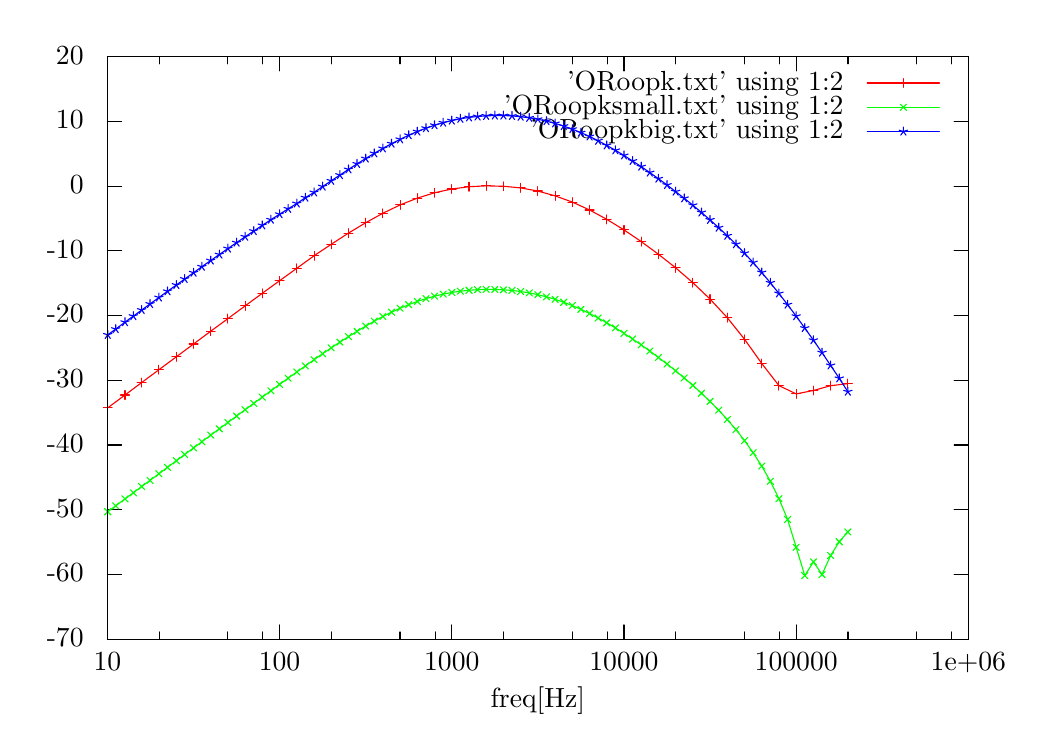
\begin{tikzpicture}[gnuplot]
%% generated with GNUPLOT 4.6p4 (Lua 5.1; terminal rev. 99, script rev. 100)
%% 2016年06月17日 17時44分48秒
\path (0.000,0.000) rectangle (12.500,8.750);
\gpcolor{color=gp lt color border}
\gpsetlinetype{gp lt border}
\gpsetlinewidth{1.00}
\draw[gp path] (1.012,0.985)--(1.192,0.985);
\draw[gp path] (11.947,0.985)--(11.767,0.985);
\node[gp node right] at (0.828,0.985) {-70};
\draw[gp path] (1.012,1.807)--(1.192,1.807);
\draw[gp path] (11.947,1.807)--(11.767,1.807);
\node[gp node right] at (0.828,1.807) {-60};
\draw[gp path] (1.012,2.629)--(1.192,2.629);
\draw[gp path] (11.947,2.629)--(11.767,2.629);
\node[gp node right] at (0.828,2.629) {-50};
\draw[gp path] (1.012,3.450)--(1.192,3.450);
\draw[gp path] (11.947,3.450)--(11.767,3.450);
\node[gp node right] at (0.828,3.450) {-40};
\draw[gp path] (1.012,4.272)--(1.192,4.272);
\draw[gp path] (11.947,4.272)--(11.767,4.272);
\node[gp node right] at (0.828,4.272) {-30};
\draw[gp path] (1.012,5.094)--(1.192,5.094);
\draw[gp path] (11.947,5.094)--(11.767,5.094);
\node[gp node right] at (0.828,5.094) {-20};
\draw[gp path] (1.012,5.916)--(1.192,5.916);
\draw[gp path] (11.947,5.916)--(11.767,5.916);
\node[gp node right] at (0.828,5.916) {-10};
\draw[gp path] (1.012,6.737)--(1.192,6.737);
\draw[gp path] (11.947,6.737)--(11.767,6.737);
\node[gp node right] at (0.828,6.737) { 0};
\draw[gp path] (1.012,7.559)--(1.192,7.559);
\draw[gp path] (11.947,7.559)--(11.767,7.559);
\node[gp node right] at (0.828,7.559) { 10};
\draw[gp path] (1.012,8.381)--(1.192,8.381);
\draw[gp path] (11.947,8.381)--(11.767,8.381);
\node[gp node right] at (0.828,8.381) { 20};
\draw[gp path] (1.012,0.985)--(1.012,1.165);
\draw[gp path] (1.012,8.381)--(1.012,8.201);
\node[gp node center] at (1.012,0.677) { 10};
\draw[gp path] (1.670,0.985)--(1.670,1.075);
\draw[gp path] (1.670,8.381)--(1.670,8.291);
\draw[gp path] (2.541,0.985)--(2.541,1.075);
\draw[gp path] (2.541,8.381)--(2.541,8.291);
\draw[gp path] (2.987,0.985)--(2.987,1.075);
\draw[gp path] (2.987,8.381)--(2.987,8.291);
\draw[gp path] (3.199,0.985)--(3.199,1.165);
\draw[gp path] (3.199,8.381)--(3.199,8.201);
\node[gp node center] at (3.199,0.677) { 100};
\draw[gp path] (3.857,0.985)--(3.857,1.075);
\draw[gp path] (3.857,8.381)--(3.857,8.291);
\draw[gp path] (4.728,0.985)--(4.728,1.075);
\draw[gp path] (4.728,8.381)--(4.728,8.291);
\draw[gp path] (5.174,0.985)--(5.174,1.075);
\draw[gp path] (5.174,8.381)--(5.174,8.291);
\draw[gp path] (5.386,0.985)--(5.386,1.165);
\draw[gp path] (5.386,8.381)--(5.386,8.201);
\node[gp node center] at (5.386,0.677) { 1000};
\draw[gp path] (6.044,0.985)--(6.044,1.075);
\draw[gp path] (6.044,8.381)--(6.044,8.291);
\draw[gp path] (6.915,0.985)--(6.915,1.075);
\draw[gp path] (6.915,8.381)--(6.915,8.291);
\draw[gp path] (7.361,0.985)--(7.361,1.075);
\draw[gp path] (7.361,8.381)--(7.361,8.291);
\draw[gp path] (7.573,0.985)--(7.573,1.165);
\draw[gp path] (7.573,8.381)--(7.573,8.201);
\node[gp node center] at (7.573,0.677) { 10000};
\draw[gp path] (8.231,0.985)--(8.231,1.075);
\draw[gp path] (8.231,8.381)--(8.231,8.291);
\draw[gp path] (9.102,0.985)--(9.102,1.075);
\draw[gp path] (9.102,8.381)--(9.102,8.291);
\draw[gp path] (9.548,0.985)--(9.548,1.075);
\draw[gp path] (9.548,8.381)--(9.548,8.291);
\draw[gp path] (9.760,0.985)--(9.760,1.165);
\draw[gp path] (9.760,8.381)--(9.760,8.201);
\node[gp node center] at (9.760,0.677) { 100000};
\draw[gp path] (10.418,0.985)--(10.418,1.075);
\draw[gp path] (10.418,8.381)--(10.418,8.291);
\draw[gp path] (11.289,0.985)--(11.289,1.075);
\draw[gp path] (11.289,8.381)--(11.289,8.291);
\draw[gp path] (11.735,0.985)--(11.735,1.075);
\draw[gp path] (11.735,8.381)--(11.735,8.291);
\draw[gp path] (11.947,0.985)--(11.947,1.165);
\draw[gp path] (11.947,8.381)--(11.947,8.201);
\node[gp node center] at (11.947,0.677) { 1e+06};
\draw[gp path] (1.012,8.381)--(1.012,0.985)--(11.947,0.985)--(11.947,8.381)--cycle;
\node[gp node center] at (6.479,0.215) {freq[Hz]};
\node[gp node right] at (10.479,8.047) {'ORoopk.txt' using 1:2};
\gpcolor{color=gp lt color 0}
\gpsetlinetype{gp lt plot 0}
\draw[gp path] (10.663,8.047)--(11.579,8.047);
\draw[gp path] (1.017,3.922)--(1.236,4.085)--(1.448,4.243)--(1.667,4.406)--(1.888,4.570)%
  --(2.107,4.733)--(2.325,4.895)--(2.543,5.055)--(2.762,5.217)--(2.979,5.376)--(3.199,5.536)%
  --(3.418,5.694)--(3.637,5.853)--(3.855,5.999)--(4.074,6.141)--(4.293,6.273)--(4.511,6.393)%
  --(4.730,6.499)--(4.948,6.585)--(5.167,6.653)--(5.386,6.701)--(5.605,6.730)--(5.823,6.741)%
  --(6.042,6.736)--(6.261,6.715)--(6.479,6.675)--(6.698,6.614)--(6.917,6.535)--(7.136,6.435)%
  --(7.354,6.316)--(7.573,6.182)--(7.792,6.033)--(8.010,5.873)--(8.229,5.700)--(8.448,5.511)%
  --(8.666,5.303)--(8.885,5.067)--(9.104,4.793)--(9.323,4.485)--(9.541,4.204)--(9.760,4.099)%
  --(9.979,4.142)--(10.197,4.203)--(10.416,4.229);
\gpsetpointsize{4.00}
\gppoint{gp mark 1}{(1.017,3.922)}
\gppoint{gp mark 1}{(1.236,4.085)}
\gppoint{gp mark 1}{(1.448,4.243)}
\gppoint{gp mark 1}{(1.667,4.406)}
\gppoint{gp mark 1}{(1.888,4.570)}
\gppoint{gp mark 1}{(2.107,4.733)}
\gppoint{gp mark 1}{(2.325,4.895)}
\gppoint{gp mark 1}{(2.543,5.055)}
\gppoint{gp mark 1}{(2.762,5.217)}
\gppoint{gp mark 1}{(2.979,5.376)}
\gppoint{gp mark 1}{(3.199,5.536)}
\gppoint{gp mark 1}{(3.418,5.694)}
\gppoint{gp mark 1}{(3.637,5.853)}
\gppoint{gp mark 1}{(3.855,5.999)}
\gppoint{gp mark 1}{(4.074,6.141)}
\gppoint{gp mark 1}{(4.293,6.273)}
\gppoint{gp mark 1}{(4.511,6.393)}
\gppoint{gp mark 1}{(4.730,6.499)}
\gppoint{gp mark 1}{(4.948,6.585)}
\gppoint{gp mark 1}{(5.167,6.653)}
\gppoint{gp mark 1}{(5.386,6.701)}
\gppoint{gp mark 1}{(5.605,6.730)}
\gppoint{gp mark 1}{(5.823,6.741)}
\gppoint{gp mark 1}{(6.042,6.736)}
\gppoint{gp mark 1}{(6.261,6.715)}
\gppoint{gp mark 1}{(6.479,6.675)}
\gppoint{gp mark 1}{(6.698,6.614)}
\gppoint{gp mark 1}{(6.917,6.535)}
\gppoint{gp mark 1}{(7.136,6.435)}
\gppoint{gp mark 1}{(7.354,6.316)}
\gppoint{gp mark 1}{(7.573,6.182)}
\gppoint{gp mark 1}{(7.792,6.033)}
\gppoint{gp mark 1}{(8.010,5.873)}
\gppoint{gp mark 1}{(8.229,5.700)}
\gppoint{gp mark 1}{(8.448,5.511)}
\gppoint{gp mark 1}{(8.666,5.303)}
\gppoint{gp mark 1}{(8.885,5.067)}
\gppoint{gp mark 1}{(9.104,4.793)}
\gppoint{gp mark 1}{(9.323,4.485)}
\gppoint{gp mark 1}{(9.541,4.204)}
\gppoint{gp mark 1}{(9.760,4.099)}
\gppoint{gp mark 1}{(9.979,4.142)}
\gppoint{gp mark 1}{(10.197,4.203)}
\gppoint{gp mark 1}{(10.416,4.229)}
\gppoint{gp mark 1}{(11.121,8.047)}
\gpcolor{color=gp lt color border}
\node[gp node right] at (10.479,7.739) {'ORoopksmall.txt' using 1:2};
\gpcolor{color=gp lt color 1}
\gpsetlinetype{gp lt plot 1}
\draw[gp path] (10.663,7.739)--(11.579,7.739);
\draw[gp path] (1.017,2.602)--(1.118,2.677)--(1.236,2.765)--(1.342,2.843)--(1.448,2.923)%
  --(1.554,3.001)--(1.667,3.085)--(1.776,3.166)--(1.888,3.250)--(1.994,3.329)--(2.107,3.413)%
  --(2.212,3.491)--(2.325,3.575)--(2.434,3.655)--(2.543,3.736)--(2.653,3.817)--(2.762,3.898)%
  --(2.871,3.978)--(2.979,4.058)--(3.089,4.138)--(3.199,4.219)--(3.308,4.298)--(3.418,4.377)%
  --(3.527,4.454)--(3.637,4.533)--(3.746,4.609)--(3.855,4.683)--(3.965,4.756)--(4.074,4.826)%
  --(4.183,4.894)--(4.293,4.960)--(4.402,5.023)--(4.511,5.082)--(4.621,5.136)--(4.730,5.187)%
  --(4.839,5.232)--(4.948,5.273)--(5.058,5.309)--(5.167,5.340)--(5.277,5.366)--(5.386,5.387)%
  --(5.495,5.403)--(5.605,5.415)--(5.714,5.423)--(5.823,5.426)--(5.933,5.426)--(6.042,5.421)%
  --(6.151,5.413)--(6.261,5.399)--(6.370,5.382)--(6.479,5.359)--(6.589,5.332)--(6.698,5.300)%
  --(6.808,5.263)--(6.917,5.220)--(7.026,5.173)--(7.136,5.120)--(7.245,5.063)--(7.354,5.002)%
  --(7.464,4.937)--(7.573,4.868)--(7.682,4.796)--(7.792,4.721)--(7.901,4.643)--(8.010,4.562)%
  --(8.120,4.478)--(8.229,4.392)--(8.338,4.301)--(8.448,4.207)--(8.557,4.107)--(8.666,4.003)%
  --(8.776,3.892)--(8.885,3.773)--(8.995,3.645)--(9.104,3.506)--(9.213,3.352)--(9.323,3.182)%
  --(9.432,2.989)--(9.541,2.768)--(9.651,2.504)--(9.760,2.151)--(9.869,1.791)--(9.979,1.966)%
  --(10.088,1.805)--(10.197,2.046)--(10.307,2.221)--(10.416,2.346);
\gppoint{gp mark 2}{(1.017,2.602)}
\gppoint{gp mark 2}{(1.118,2.677)}
\gppoint{gp mark 2}{(1.236,2.765)}
\gppoint{gp mark 2}{(1.342,2.843)}
\gppoint{gp mark 2}{(1.448,2.923)}
\gppoint{gp mark 2}{(1.554,3.001)}
\gppoint{gp mark 2}{(1.667,3.085)}
\gppoint{gp mark 2}{(1.776,3.166)}
\gppoint{gp mark 2}{(1.888,3.250)}
\gppoint{gp mark 2}{(1.994,3.329)}
\gppoint{gp mark 2}{(2.107,3.413)}
\gppoint{gp mark 2}{(2.212,3.491)}
\gppoint{gp mark 2}{(2.325,3.575)}
\gppoint{gp mark 2}{(2.434,3.655)}
\gppoint{gp mark 2}{(2.543,3.736)}
\gppoint{gp mark 2}{(2.653,3.817)}
\gppoint{gp mark 2}{(2.762,3.898)}
\gppoint{gp mark 2}{(2.871,3.978)}
\gppoint{gp mark 2}{(2.979,4.058)}
\gppoint{gp mark 2}{(3.089,4.138)}
\gppoint{gp mark 2}{(3.199,4.219)}
\gppoint{gp mark 2}{(3.308,4.298)}
\gppoint{gp mark 2}{(3.418,4.377)}
\gppoint{gp mark 2}{(3.527,4.454)}
\gppoint{gp mark 2}{(3.637,4.533)}
\gppoint{gp mark 2}{(3.746,4.609)}
\gppoint{gp mark 2}{(3.855,4.683)}
\gppoint{gp mark 2}{(3.965,4.756)}
\gppoint{gp mark 2}{(4.074,4.826)}
\gppoint{gp mark 2}{(4.183,4.894)}
\gppoint{gp mark 2}{(4.293,4.960)}
\gppoint{gp mark 2}{(4.402,5.023)}
\gppoint{gp mark 2}{(4.511,5.082)}
\gppoint{gp mark 2}{(4.621,5.136)}
\gppoint{gp mark 2}{(4.730,5.187)}
\gppoint{gp mark 2}{(4.839,5.232)}
\gppoint{gp mark 2}{(4.948,5.273)}
\gppoint{gp mark 2}{(5.058,5.309)}
\gppoint{gp mark 2}{(5.167,5.340)}
\gppoint{gp mark 2}{(5.277,5.366)}
\gppoint{gp mark 2}{(5.386,5.387)}
\gppoint{gp mark 2}{(5.495,5.403)}
\gppoint{gp mark 2}{(5.605,5.415)}
\gppoint{gp mark 2}{(5.714,5.423)}
\gppoint{gp mark 2}{(5.823,5.426)}
\gppoint{gp mark 2}{(5.933,5.426)}
\gppoint{gp mark 2}{(6.042,5.421)}
\gppoint{gp mark 2}{(6.151,5.413)}
\gppoint{gp mark 2}{(6.261,5.399)}
\gppoint{gp mark 2}{(6.370,5.382)}
\gppoint{gp mark 2}{(6.479,5.359)}
\gppoint{gp mark 2}{(6.589,5.332)}
\gppoint{gp mark 2}{(6.698,5.300)}
\gppoint{gp mark 2}{(6.808,5.263)}
\gppoint{gp mark 2}{(6.917,5.220)}
\gppoint{gp mark 2}{(7.026,5.173)}
\gppoint{gp mark 2}{(7.136,5.120)}
\gppoint{gp mark 2}{(7.245,5.063)}
\gppoint{gp mark 2}{(7.354,5.002)}
\gppoint{gp mark 2}{(7.464,4.937)}
\gppoint{gp mark 2}{(7.573,4.868)}
\gppoint{gp mark 2}{(7.682,4.796)}
\gppoint{gp mark 2}{(7.792,4.721)}
\gppoint{gp mark 2}{(7.901,4.643)}
\gppoint{gp mark 2}{(8.010,4.562)}
\gppoint{gp mark 2}{(8.120,4.478)}
\gppoint{gp mark 2}{(8.229,4.392)}
\gppoint{gp mark 2}{(8.338,4.301)}
\gppoint{gp mark 2}{(8.448,4.207)}
\gppoint{gp mark 2}{(8.557,4.107)}
\gppoint{gp mark 2}{(8.666,4.003)}
\gppoint{gp mark 2}{(8.776,3.892)}
\gppoint{gp mark 2}{(8.885,3.773)}
\gppoint{gp mark 2}{(8.995,3.645)}
\gppoint{gp mark 2}{(9.104,3.506)}
\gppoint{gp mark 2}{(9.213,3.352)}
\gppoint{gp mark 2}{(9.323,3.182)}
\gppoint{gp mark 2}{(9.432,2.989)}
\gppoint{gp mark 2}{(9.541,2.768)}
\gppoint{gp mark 2}{(9.651,2.504)}
\gppoint{gp mark 2}{(9.760,2.151)}
\gppoint{gp mark 2}{(9.869,1.791)}
\gppoint{gp mark 2}{(9.979,1.966)}
\gppoint{gp mark 2}{(10.088,1.805)}
\gppoint{gp mark 2}{(10.197,2.046)}
\gppoint{gp mark 2}{(10.307,2.221)}
\gppoint{gp mark 2}{(10.416,2.346)}
\gppoint{gp mark 2}{(11.121,7.739)}
\gpcolor{color=gp lt color border}
\node[gp node right] at (10.479,7.431) {'ORoopkbig.txt' using 1:2};
\gpcolor{color=gp lt color 2}
\gpsetlinetype{gp lt plot 2}
\draw[gp path] (10.663,7.431)--(11.579,7.431);
\draw[gp path] (1.017,4.849)--(1.118,4.922)--(1.236,5.010)--(1.342,5.087)--(1.448,5.164)%
  --(1.554,5.241)--(1.667,5.323)--(1.776,5.402)--(1.888,5.482)--(1.994,5.558)--(2.107,5.638)%
  --(2.212,5.714)--(2.325,5.793)--(2.434,5.869)--(2.543,5.945)--(2.653,6.020)--(2.762,6.095)%
  --(2.871,6.167)--(2.979,6.239)--(3.089,6.311)--(3.199,6.381)--(3.308,6.449)--(3.418,6.517)%
  --(3.527,6.591)--(3.637,6.658)--(3.746,6.732)--(3.855,6.805)--(3.965,6.878)--(4.074,6.950)%
  --(4.183,7.020)--(4.293,7.088)--(4.402,7.154)--(4.511,7.217)--(4.621,7.277)--(4.730,7.332)%
  --(4.839,7.384)--(4.948,7.431)--(5.058,7.474)--(5.167,7.511)--(5.277,7.543)--(5.386,7.570)%
  --(5.495,7.593)--(5.605,7.610)--(5.714,7.622)--(5.823,7.630)--(5.933,7.634)--(6.042,7.634)%
  --(6.151,7.629)--(6.261,7.619)--(6.370,7.605)--(6.479,7.587)--(6.589,7.563)--(6.698,7.534)%
  --(6.808,7.500)--(6.917,7.461)--(7.026,7.417)--(7.136,7.368)--(7.245,7.314)--(7.354,7.255)%
  --(7.464,7.193)--(7.573,7.127)--(7.682,7.057)--(7.792,6.985)--(7.901,6.910)--(8.010,6.832)%
  --(8.120,6.752)--(8.229,6.668)--(8.338,6.583)--(8.448,6.495)--(8.557,6.403)--(8.666,6.309)%
  --(8.776,6.210)--(8.885,6.107)--(8.995,5.999)--(9.104,5.886)--(9.213,5.767)--(9.323,5.641)%
  --(9.432,5.510)--(9.541,5.374)--(9.651,5.232)--(9.760,5.086)--(9.869,4.935)--(9.979,4.781)%
  --(10.088,4.623)--(10.197,4.461)--(10.307,4.296)--(10.416,4.127);
\gppoint{gp mark 3}{(1.017,4.849)}
\gppoint{gp mark 3}{(1.118,4.922)}
\gppoint{gp mark 3}{(1.236,5.010)}
\gppoint{gp mark 3}{(1.342,5.087)}
\gppoint{gp mark 3}{(1.448,5.164)}
\gppoint{gp mark 3}{(1.554,5.241)}
\gppoint{gp mark 3}{(1.667,5.323)}
\gppoint{gp mark 3}{(1.776,5.402)}
\gppoint{gp mark 3}{(1.888,5.482)}
\gppoint{gp mark 3}{(1.994,5.558)}
\gppoint{gp mark 3}{(2.107,5.638)}
\gppoint{gp mark 3}{(2.212,5.714)}
\gppoint{gp mark 3}{(2.325,5.793)}
\gppoint{gp mark 3}{(2.434,5.869)}
\gppoint{gp mark 3}{(2.543,5.945)}
\gppoint{gp mark 3}{(2.653,6.020)}
\gppoint{gp mark 3}{(2.762,6.095)}
\gppoint{gp mark 3}{(2.871,6.167)}
\gppoint{gp mark 3}{(2.979,6.239)}
\gppoint{gp mark 3}{(3.089,6.311)}
\gppoint{gp mark 3}{(3.199,6.381)}
\gppoint{gp mark 3}{(3.308,6.449)}
\gppoint{gp mark 3}{(3.418,6.517)}
\gppoint{gp mark 3}{(3.527,6.591)}
\gppoint{gp mark 3}{(3.637,6.658)}
\gppoint{gp mark 3}{(3.746,6.732)}
\gppoint{gp mark 3}{(3.855,6.805)}
\gppoint{gp mark 3}{(3.965,6.878)}
\gppoint{gp mark 3}{(4.074,6.950)}
\gppoint{gp mark 3}{(4.183,7.020)}
\gppoint{gp mark 3}{(4.293,7.088)}
\gppoint{gp mark 3}{(4.402,7.154)}
\gppoint{gp mark 3}{(4.511,7.217)}
\gppoint{gp mark 3}{(4.621,7.277)}
\gppoint{gp mark 3}{(4.730,7.332)}
\gppoint{gp mark 3}{(4.839,7.384)}
\gppoint{gp mark 3}{(4.948,7.431)}
\gppoint{gp mark 3}{(5.058,7.474)}
\gppoint{gp mark 3}{(5.167,7.511)}
\gppoint{gp mark 3}{(5.277,7.543)}
\gppoint{gp mark 3}{(5.386,7.570)}
\gppoint{gp mark 3}{(5.495,7.593)}
\gppoint{gp mark 3}{(5.605,7.610)}
\gppoint{gp mark 3}{(5.714,7.622)}
\gppoint{gp mark 3}{(5.823,7.630)}
\gppoint{gp mark 3}{(5.933,7.634)}
\gppoint{gp mark 3}{(6.042,7.634)}
\gppoint{gp mark 3}{(6.151,7.629)}
\gppoint{gp mark 3}{(6.261,7.619)}
\gppoint{gp mark 3}{(6.370,7.605)}
\gppoint{gp mark 3}{(6.479,7.587)}
\gppoint{gp mark 3}{(6.589,7.563)}
\gppoint{gp mark 3}{(6.698,7.534)}
\gppoint{gp mark 3}{(6.808,7.500)}
\gppoint{gp mark 3}{(6.917,7.461)}
\gppoint{gp mark 3}{(7.026,7.417)}
\gppoint{gp mark 3}{(7.136,7.368)}
\gppoint{gp mark 3}{(7.245,7.314)}
\gppoint{gp mark 3}{(7.354,7.255)}
\gppoint{gp mark 3}{(7.464,7.193)}
\gppoint{gp mark 3}{(7.573,7.127)}
\gppoint{gp mark 3}{(7.682,7.057)}
\gppoint{gp mark 3}{(7.792,6.985)}
\gppoint{gp mark 3}{(7.901,6.910)}
\gppoint{gp mark 3}{(8.010,6.832)}
\gppoint{gp mark 3}{(8.120,6.752)}
\gppoint{gp mark 3}{(8.229,6.668)}
\gppoint{gp mark 3}{(8.338,6.583)}
\gppoint{gp mark 3}{(8.448,6.495)}
\gppoint{gp mark 3}{(8.557,6.403)}
\gppoint{gp mark 3}{(8.666,6.309)}
\gppoint{gp mark 3}{(8.776,6.210)}
\gppoint{gp mark 3}{(8.885,6.107)}
\gppoint{gp mark 3}{(8.995,5.999)}
\gppoint{gp mark 3}{(9.104,5.886)}
\gppoint{gp mark 3}{(9.213,5.767)}
\gppoint{gp mark 3}{(9.323,5.641)}
\gppoint{gp mark 3}{(9.432,5.510)}
\gppoint{gp mark 3}{(9.541,5.374)}
\gppoint{gp mark 3}{(9.651,5.232)}
\gppoint{gp mark 3}{(9.760,5.086)}
\gppoint{gp mark 3}{(9.869,4.935)}
\gppoint{gp mark 3}{(9.979,4.781)}
\gppoint{gp mark 3}{(10.088,4.623)}
\gppoint{gp mark 3}{(10.197,4.461)}
\gppoint{gp mark 3}{(10.307,4.296)}
\gppoint{gp mark 3}{(10.416,4.127)}
\gppoint{gp mark 3}{(11.121,7.431)}
\gpcolor{color=gp lt color border}
\gpsetlinetype{gp lt border}
\draw[gp path] (1.012,8.381)--(1.012,0.985)--(11.947,0.985)--(11.947,8.381)--cycle;
%% coordinates of the plot area
\gpdefrectangularnode{gp plot 1}{\pgfpoint{1.012cm}{0.985cm}}{\pgfpoint{11.947cm}{8.381cm}}
\end{tikzpicture}
%% gnuplot variables
}
        \caption{発振回路(開ループ)の振幅特性}
      \end{minipage} &
      %---- 2番目の図 --------------------------
      \begin{minipage}[t]{0.45\hsize}
        \centering
        \scalebox{0.65}{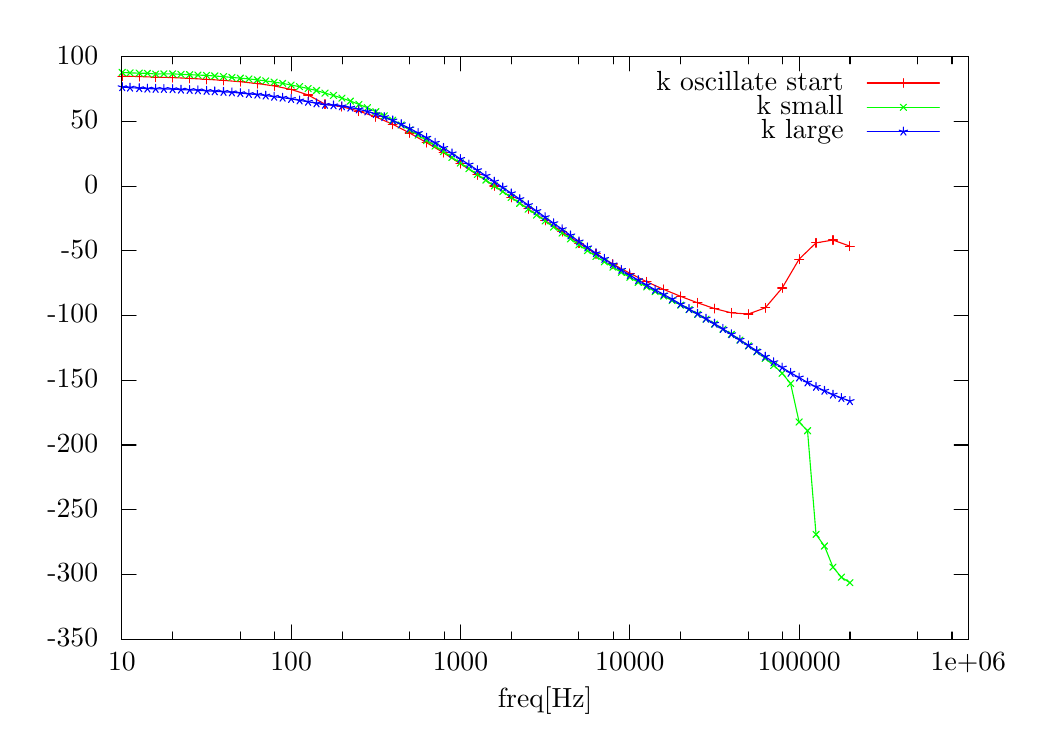
\begin{tikzpicture}[gnuplot]
%% generated with GNUPLOT 4.6p4 (Lua 5.1; terminal rev. 99, script rev. 100)
%% 2016年06月17日 17時49分40秒
\path (0.000,0.000) rectangle (12.500,8.750);
\gpcolor{color=gp lt color border}
\gpsetlinetype{gp lt border}
\gpsetlinewidth{1.00}
\draw[gp path] (1.196,0.985)--(1.376,0.985);
\draw[gp path] (11.947,0.985)--(11.767,0.985);
\node[gp node right] at (1.012,0.985) {-350};
\draw[gp path] (1.196,1.807)--(1.376,1.807);
\draw[gp path] (11.947,1.807)--(11.767,1.807);
\node[gp node right] at (1.012,1.807) {-300};
\draw[gp path] (1.196,2.629)--(1.376,2.629);
\draw[gp path] (11.947,2.629)--(11.767,2.629);
\node[gp node right] at (1.012,2.629) {-250};
\draw[gp path] (1.196,3.450)--(1.376,3.450);
\draw[gp path] (11.947,3.450)--(11.767,3.450);
\node[gp node right] at (1.012,3.450) {-200};
\draw[gp path] (1.196,4.272)--(1.376,4.272);
\draw[gp path] (11.947,4.272)--(11.767,4.272);
\node[gp node right] at (1.012,4.272) {-150};
\draw[gp path] (1.196,5.094)--(1.376,5.094);
\draw[gp path] (11.947,5.094)--(11.767,5.094);
\node[gp node right] at (1.012,5.094) {-100};
\draw[gp path] (1.196,5.916)--(1.376,5.916);
\draw[gp path] (11.947,5.916)--(11.767,5.916);
\node[gp node right] at (1.012,5.916) {-50};
\draw[gp path] (1.196,6.737)--(1.376,6.737);
\draw[gp path] (11.947,6.737)--(11.767,6.737);
\node[gp node right] at (1.012,6.737) { 0};
\draw[gp path] (1.196,7.559)--(1.376,7.559);
\draw[gp path] (11.947,7.559)--(11.767,7.559);
\node[gp node right] at (1.012,7.559) { 50};
\draw[gp path] (1.196,8.381)--(1.376,8.381);
\draw[gp path] (11.947,8.381)--(11.767,8.381);
\node[gp node right] at (1.012,8.381) { 100};
\draw[gp path] (1.196,0.985)--(1.196,1.165);
\draw[gp path] (1.196,8.381)--(1.196,8.201);
\node[gp node center] at (1.196,0.677) { 10};
\draw[gp path] (1.843,0.985)--(1.843,1.075);
\draw[gp path] (1.843,8.381)--(1.843,8.291);
\draw[gp path] (2.699,0.985)--(2.699,1.075);
\draw[gp path] (2.699,8.381)--(2.699,8.291);
\draw[gp path] (3.138,0.985)--(3.138,1.075);
\draw[gp path] (3.138,8.381)--(3.138,8.291);
\draw[gp path] (3.346,0.985)--(3.346,1.165);
\draw[gp path] (3.346,8.381)--(3.346,8.201);
\node[gp node center] at (3.346,0.677) { 100};
\draw[gp path] (3.993,0.985)--(3.993,1.075);
\draw[gp path] (3.993,8.381)--(3.993,8.291);
\draw[gp path] (4.849,0.985)--(4.849,1.075);
\draw[gp path] (4.849,8.381)--(4.849,8.291);
\draw[gp path] (5.288,0.985)--(5.288,1.075);
\draw[gp path] (5.288,8.381)--(5.288,8.291);
\draw[gp path] (5.496,0.985)--(5.496,1.165);
\draw[gp path] (5.496,8.381)--(5.496,8.201);
\node[gp node center] at (5.496,0.677) { 1000};
\draw[gp path] (6.144,0.985)--(6.144,1.075);
\draw[gp path] (6.144,8.381)--(6.144,8.291);
\draw[gp path] (6.999,0.985)--(6.999,1.075);
\draw[gp path] (6.999,8.381)--(6.999,8.291);
\draw[gp path] (7.438,0.985)--(7.438,1.075);
\draw[gp path] (7.438,8.381)--(7.438,8.291);
\draw[gp path] (7.647,0.985)--(7.647,1.165);
\draw[gp path] (7.647,8.381)--(7.647,8.201);
\node[gp node center] at (7.647,0.677) { 10000};
\draw[gp path] (8.294,0.985)--(8.294,1.075);
\draw[gp path] (8.294,8.381)--(8.294,8.291);
\draw[gp path] (9.150,0.985)--(9.150,1.075);
\draw[gp path] (9.150,8.381)--(9.150,8.291);
\draw[gp path] (9.588,0.985)--(9.588,1.075);
\draw[gp path] (9.588,8.381)--(9.588,8.291);
\draw[gp path] (9.797,0.985)--(9.797,1.165);
\draw[gp path] (9.797,8.381)--(9.797,8.201);
\node[gp node center] at (9.797,0.677) { 100000};
\draw[gp path] (10.444,0.985)--(10.444,1.075);
\draw[gp path] (10.444,8.381)--(10.444,8.291);
\draw[gp path] (11.300,0.985)--(11.300,1.075);
\draw[gp path] (11.300,8.381)--(11.300,8.291);
\draw[gp path] (11.739,0.985)--(11.739,1.075);
\draw[gp path] (11.739,8.381)--(11.739,8.291);
\draw[gp path] (11.947,0.985)--(11.947,1.165);
\draw[gp path] (11.947,8.381)--(11.947,8.201);
\node[gp node center] at (11.947,0.677) { 1e+06};
\draw[gp path] (1.196,8.381)--(1.196,0.985)--(11.947,0.985)--(11.947,8.381)--cycle;
\node[gp node center] at (6.571,0.215) {freq[Hz]};
\node[gp node right] at (10.479,8.047) {k oscillate start};
\gpcolor{color=gp lt color 0}
\gpsetlinetype{gp lt plot 0}
\draw[gp path] (10.663,8.047)--(11.579,8.047);
\draw[gp path] (1.201,8.135)--(1.417,8.129)--(1.625,8.122)--(1.840,8.116)--(2.057,8.106)%
  --(2.272,8.094)--(2.487,8.081)--(2.701,8.063)--(2.917,8.040)--(3.130,8.010)--(3.346,7.966)%
  --(3.561,7.895)--(3.776,7.779)--(3.991,7.746)--(4.207,7.690)--(4.421,7.617)--(4.636,7.523)%
  --(4.851,7.412)--(5.066,7.290)--(5.281,7.162)--(5.496,7.022)--(5.711,6.881)--(5.926,6.739)%
  --(6.141,6.595)--(6.357,6.448)--(6.571,6.301)--(6.787,6.159)--(7.002,6.014)--(7.217,5.877)%
  --(7.432,5.748)--(7.647,5.631)--(7.862,5.523)--(8.077,5.426)--(8.292,5.338)--(8.507,5.256)%
  --(8.722,5.183)--(8.937,5.128)--(9.152,5.113)--(9.367,5.192)--(9.582,5.444)--(9.797,5.810)%
  --(10.012,6.017)--(10.227,6.053)--(10.442,5.975);
\gpsetpointsize{4.00}
\gppoint{gp mark 1}{(1.201,8.135)}
\gppoint{gp mark 1}{(1.417,8.129)}
\gppoint{gp mark 1}{(1.625,8.122)}
\gppoint{gp mark 1}{(1.840,8.116)}
\gppoint{gp mark 1}{(2.057,8.106)}
\gppoint{gp mark 1}{(2.272,8.094)}
\gppoint{gp mark 1}{(2.487,8.081)}
\gppoint{gp mark 1}{(2.701,8.063)}
\gppoint{gp mark 1}{(2.917,8.040)}
\gppoint{gp mark 1}{(3.130,8.010)}
\gppoint{gp mark 1}{(3.346,7.966)}
\gppoint{gp mark 1}{(3.561,7.895)}
\gppoint{gp mark 1}{(3.776,7.779)}
\gppoint{gp mark 1}{(3.991,7.746)}
\gppoint{gp mark 1}{(4.207,7.690)}
\gppoint{gp mark 1}{(4.421,7.617)}
\gppoint{gp mark 1}{(4.636,7.523)}
\gppoint{gp mark 1}{(4.851,7.412)}
\gppoint{gp mark 1}{(5.066,7.290)}
\gppoint{gp mark 1}{(5.281,7.162)}
\gppoint{gp mark 1}{(5.496,7.022)}
\gppoint{gp mark 1}{(5.711,6.881)}
\gppoint{gp mark 1}{(5.926,6.739)}
\gppoint{gp mark 1}{(6.141,6.595)}
\gppoint{gp mark 1}{(6.357,6.448)}
\gppoint{gp mark 1}{(6.571,6.301)}
\gppoint{gp mark 1}{(6.787,6.159)}
\gppoint{gp mark 1}{(7.002,6.014)}
\gppoint{gp mark 1}{(7.217,5.877)}
\gppoint{gp mark 1}{(7.432,5.748)}
\gppoint{gp mark 1}{(7.647,5.631)}
\gppoint{gp mark 1}{(7.862,5.523)}
\gppoint{gp mark 1}{(8.077,5.426)}
\gppoint{gp mark 1}{(8.292,5.338)}
\gppoint{gp mark 1}{(8.507,5.256)}
\gppoint{gp mark 1}{(8.722,5.183)}
\gppoint{gp mark 1}{(8.937,5.128)}
\gppoint{gp mark 1}{(9.152,5.113)}
\gppoint{gp mark 1}{(9.367,5.192)}
\gppoint{gp mark 1}{(9.582,5.444)}
\gppoint{gp mark 1}{(9.797,5.810)}
\gppoint{gp mark 1}{(10.012,6.017)}
\gppoint{gp mark 1}{(10.227,6.053)}
\gppoint{gp mark 1}{(10.442,5.975)}
\gppoint{gp mark 1}{(11.121,8.047)}
\gpcolor{color=gp lt color border}
\node[gp node right] at (10.479,7.739) {k small};
\gpcolor{color=gp lt color 1}
\gpsetlinetype{gp lt plot 1}
\draw[gp path] (10.663,7.739)--(11.579,7.739);
\draw[gp path] (1.201,8.181)--(1.300,8.176)--(1.417,8.172)--(1.521,8.170)--(1.625,8.161)%
  --(1.729,8.164)--(1.840,8.164)--(1.947,8.157)--(2.057,8.153)--(2.162,8.148)--(2.272,8.144)%
  --(2.376,8.136)--(2.487,8.128)--(2.594,8.118)--(2.701,8.109)--(2.809,8.099)--(2.917,8.087)%
  --(3.023,8.074)--(3.130,8.058)--(3.238,8.043)--(3.346,8.021)--(3.453,8.001)--(3.561,7.977)%
  --(3.668,7.952)--(3.776,7.919)--(3.884,7.889)--(3.991,7.855)--(4.099,7.818)--(4.207,7.776)%
  --(4.314,7.733)--(4.421,7.683)--(4.529,7.630)--(4.636,7.574)--(4.744,7.514)--(4.851,7.451)%
  --(4.959,7.385)--(5.066,7.317)--(5.174,7.247)--(5.281,7.176)--(5.389,7.103)--(5.496,7.031)%
  --(5.604,6.960)--(5.711,6.886)--(5.819,6.814)--(5.926,6.740)--(6.034,6.668)--(6.141,6.594)%
  --(6.249,6.520)--(6.357,6.445)--(6.464,6.371)--(6.571,6.295)--(6.679,6.218)--(6.787,6.142)%
  --(6.894,6.067)--(7.002,5.991)--(7.109,5.918)--(7.217,5.845)--(7.324,5.776)--(7.432,5.708)%
  --(7.539,5.642)--(7.647,5.579)--(7.754,5.517)--(7.862,5.457)--(7.969,5.398)--(8.077,5.341)%
  --(8.184,5.284)--(8.292,5.226)--(8.399,5.169)--(8.507,5.110)--(8.614,5.049)--(8.722,4.986)%
  --(8.829,4.921)--(8.937,4.855)--(9.044,4.783)--(9.152,4.708)--(9.259,4.633)--(9.367,4.549)%
  --(9.474,4.461)--(9.582,4.361)--(9.689,4.231)--(9.797,3.742)--(9.904,3.631)--(10.012,2.314)%
  --(10.119,2.167)--(10.227,1.899)--(10.334,1.771)--(10.442,1.701);
\gppoint{gp mark 2}{(1.201,8.181)}
\gppoint{gp mark 2}{(1.300,8.176)}
\gppoint{gp mark 2}{(1.417,8.172)}
\gppoint{gp mark 2}{(1.521,8.170)}
\gppoint{gp mark 2}{(1.625,8.161)}
\gppoint{gp mark 2}{(1.729,8.164)}
\gppoint{gp mark 2}{(1.840,8.164)}
\gppoint{gp mark 2}{(1.947,8.157)}
\gppoint{gp mark 2}{(2.057,8.153)}
\gppoint{gp mark 2}{(2.162,8.148)}
\gppoint{gp mark 2}{(2.272,8.144)}
\gppoint{gp mark 2}{(2.376,8.136)}
\gppoint{gp mark 2}{(2.487,8.128)}
\gppoint{gp mark 2}{(2.594,8.118)}
\gppoint{gp mark 2}{(2.701,8.109)}
\gppoint{gp mark 2}{(2.809,8.099)}
\gppoint{gp mark 2}{(2.917,8.087)}
\gppoint{gp mark 2}{(3.023,8.074)}
\gppoint{gp mark 2}{(3.130,8.058)}
\gppoint{gp mark 2}{(3.238,8.043)}
\gppoint{gp mark 2}{(3.346,8.021)}
\gppoint{gp mark 2}{(3.453,8.001)}
\gppoint{gp mark 2}{(3.561,7.977)}
\gppoint{gp mark 2}{(3.668,7.952)}
\gppoint{gp mark 2}{(3.776,7.919)}
\gppoint{gp mark 2}{(3.884,7.889)}
\gppoint{gp mark 2}{(3.991,7.855)}
\gppoint{gp mark 2}{(4.099,7.818)}
\gppoint{gp mark 2}{(4.207,7.776)}
\gppoint{gp mark 2}{(4.314,7.733)}
\gppoint{gp mark 2}{(4.421,7.683)}
\gppoint{gp mark 2}{(4.529,7.630)}
\gppoint{gp mark 2}{(4.636,7.574)}
\gppoint{gp mark 2}{(4.744,7.514)}
\gppoint{gp mark 2}{(4.851,7.451)}
\gppoint{gp mark 2}{(4.959,7.385)}
\gppoint{gp mark 2}{(5.066,7.317)}
\gppoint{gp mark 2}{(5.174,7.247)}
\gppoint{gp mark 2}{(5.281,7.176)}
\gppoint{gp mark 2}{(5.389,7.103)}
\gppoint{gp mark 2}{(5.496,7.031)}
\gppoint{gp mark 2}{(5.604,6.960)}
\gppoint{gp mark 2}{(5.711,6.886)}
\gppoint{gp mark 2}{(5.819,6.814)}
\gppoint{gp mark 2}{(5.926,6.740)}
\gppoint{gp mark 2}{(6.034,6.668)}
\gppoint{gp mark 2}{(6.141,6.594)}
\gppoint{gp mark 2}{(6.249,6.520)}
\gppoint{gp mark 2}{(6.357,6.445)}
\gppoint{gp mark 2}{(6.464,6.371)}
\gppoint{gp mark 2}{(6.571,6.295)}
\gppoint{gp mark 2}{(6.679,6.218)}
\gppoint{gp mark 2}{(6.787,6.142)}
\gppoint{gp mark 2}{(6.894,6.067)}
\gppoint{gp mark 2}{(7.002,5.991)}
\gppoint{gp mark 2}{(7.109,5.918)}
\gppoint{gp mark 2}{(7.217,5.845)}
\gppoint{gp mark 2}{(7.324,5.776)}
\gppoint{gp mark 2}{(7.432,5.708)}
\gppoint{gp mark 2}{(7.539,5.642)}
\gppoint{gp mark 2}{(7.647,5.579)}
\gppoint{gp mark 2}{(7.754,5.517)}
\gppoint{gp mark 2}{(7.862,5.457)}
\gppoint{gp mark 2}{(7.969,5.398)}
\gppoint{gp mark 2}{(8.077,5.341)}
\gppoint{gp mark 2}{(8.184,5.284)}
\gppoint{gp mark 2}{(8.292,5.226)}
\gppoint{gp mark 2}{(8.399,5.169)}
\gppoint{gp mark 2}{(8.507,5.110)}
\gppoint{gp mark 2}{(8.614,5.049)}
\gppoint{gp mark 2}{(8.722,4.986)}
\gppoint{gp mark 2}{(8.829,4.921)}
\gppoint{gp mark 2}{(8.937,4.855)}
\gppoint{gp mark 2}{(9.044,4.783)}
\gppoint{gp mark 2}{(9.152,4.708)}
\gppoint{gp mark 2}{(9.259,4.633)}
\gppoint{gp mark 2}{(9.367,4.549)}
\gppoint{gp mark 2}{(9.474,4.461)}
\gppoint{gp mark 2}{(9.582,4.361)}
\gppoint{gp mark 2}{(9.689,4.231)}
\gppoint{gp mark 2}{(9.797,3.742)}
\gppoint{gp mark 2}{(9.904,3.631)}
\gppoint{gp mark 2}{(10.012,2.314)}
\gppoint{gp mark 2}{(10.119,2.167)}
\gppoint{gp mark 2}{(10.227,1.899)}
\gppoint{gp mark 2}{(10.334,1.771)}
\gppoint{gp mark 2}{(10.442,1.701)}
\gppoint{gp mark 2}{(11.121,7.739)}
\gpcolor{color=gp lt color border}
\node[gp node right] at (10.479,7.431) {k large};
\gpcolor{color=gp lt color 2}
\gpsetlinetype{gp lt plot 2}
\draw[gp path] (10.663,7.431)--(11.579,7.431);
\draw[gp path] (1.201,7.994)--(1.300,7.989)--(1.417,7.981)--(1.521,7.976)--(1.625,7.973)%
  --(1.729,7.972)--(1.840,7.969)--(1.947,7.963)--(2.057,7.959)--(2.162,7.955)--(2.272,7.947)%
  --(2.376,7.942)--(2.487,7.935)--(2.594,7.929)--(2.701,7.919)--(2.809,7.908)--(2.917,7.900)%
  --(3.023,7.888)--(3.130,7.873)--(3.238,7.861)--(3.346,7.845)--(3.453,7.826)--(3.561,7.809)%
  --(3.668,7.789)--(3.776,7.771)--(3.884,7.764)--(3.991,7.752)--(4.099,7.735)--(4.207,7.713)%
  --(4.314,7.686)--(4.421,7.653)--(4.529,7.614)--(4.636,7.572)--(4.744,7.524)--(4.851,7.471)%
  --(4.959,7.413)--(5.066,7.353)--(5.174,7.289)--(5.281,7.223)--(5.389,7.154)--(5.496,7.083)%
  --(5.604,7.012)--(5.711,6.941)--(5.819,6.869)--(5.926,6.795)--(6.034,6.721)--(6.141,6.647)%
  --(6.249,6.573)--(6.357,6.497)--(6.464,6.421)--(6.571,6.344)--(6.679,6.267)--(6.787,6.191)%
  --(6.894,6.112)--(7.002,6.035)--(7.109,5.960)--(7.217,5.886)--(7.324,5.814)--(7.432,5.744)%
  --(7.539,5.674)--(7.647,5.608)--(7.754,5.544)--(7.862,5.482)--(7.969,5.421)--(8.077,5.362)%
  --(8.184,5.303)--(8.292,5.238)--(8.399,5.178)--(8.507,5.117)--(8.614,5.055)--(8.722,4.991)%
  --(8.829,4.925)--(8.937,4.857)--(9.044,4.787)--(9.152,4.716)--(9.259,4.645)--(9.367,4.571)%
  --(9.474,4.502)--(9.582,4.434)--(9.689,4.367)--(9.797,4.307)--(9.904,4.244)--(10.012,4.189)%
  --(10.119,4.139)--(10.227,4.090)--(10.334,4.047)--(10.442,4.008);
\gppoint{gp mark 3}{(1.201,7.994)}
\gppoint{gp mark 3}{(1.300,7.989)}
\gppoint{gp mark 3}{(1.417,7.981)}
\gppoint{gp mark 3}{(1.521,7.976)}
\gppoint{gp mark 3}{(1.625,7.973)}
\gppoint{gp mark 3}{(1.729,7.972)}
\gppoint{gp mark 3}{(1.840,7.969)}
\gppoint{gp mark 3}{(1.947,7.963)}
\gppoint{gp mark 3}{(2.057,7.959)}
\gppoint{gp mark 3}{(2.162,7.955)}
\gppoint{gp mark 3}{(2.272,7.947)}
\gppoint{gp mark 3}{(2.376,7.942)}
\gppoint{gp mark 3}{(2.487,7.935)}
\gppoint{gp mark 3}{(2.594,7.929)}
\gppoint{gp mark 3}{(2.701,7.919)}
\gppoint{gp mark 3}{(2.809,7.908)}
\gppoint{gp mark 3}{(2.917,7.900)}
\gppoint{gp mark 3}{(3.023,7.888)}
\gppoint{gp mark 3}{(3.130,7.873)}
\gppoint{gp mark 3}{(3.238,7.861)}
\gppoint{gp mark 3}{(3.346,7.845)}
\gppoint{gp mark 3}{(3.453,7.826)}
\gppoint{gp mark 3}{(3.561,7.809)}
\gppoint{gp mark 3}{(3.668,7.789)}
\gppoint{gp mark 3}{(3.776,7.771)}
\gppoint{gp mark 3}{(3.884,7.764)}
\gppoint{gp mark 3}{(3.991,7.752)}
\gppoint{gp mark 3}{(4.099,7.735)}
\gppoint{gp mark 3}{(4.207,7.713)}
\gppoint{gp mark 3}{(4.314,7.686)}
\gppoint{gp mark 3}{(4.421,7.653)}
\gppoint{gp mark 3}{(4.529,7.614)}
\gppoint{gp mark 3}{(4.636,7.572)}
\gppoint{gp mark 3}{(4.744,7.524)}
\gppoint{gp mark 3}{(4.851,7.471)}
\gppoint{gp mark 3}{(4.959,7.413)}
\gppoint{gp mark 3}{(5.066,7.353)}
\gppoint{gp mark 3}{(5.174,7.289)}
\gppoint{gp mark 3}{(5.281,7.223)}
\gppoint{gp mark 3}{(5.389,7.154)}
\gppoint{gp mark 3}{(5.496,7.083)}
\gppoint{gp mark 3}{(5.604,7.012)}
\gppoint{gp mark 3}{(5.711,6.941)}
\gppoint{gp mark 3}{(5.819,6.869)}
\gppoint{gp mark 3}{(5.926,6.795)}
\gppoint{gp mark 3}{(6.034,6.721)}
\gppoint{gp mark 3}{(6.141,6.647)}
\gppoint{gp mark 3}{(6.249,6.573)}
\gppoint{gp mark 3}{(6.357,6.497)}
\gppoint{gp mark 3}{(6.464,6.421)}
\gppoint{gp mark 3}{(6.571,6.344)}
\gppoint{gp mark 3}{(6.679,6.267)}
\gppoint{gp mark 3}{(6.787,6.191)}
\gppoint{gp mark 3}{(6.894,6.112)}
\gppoint{gp mark 3}{(7.002,6.035)}
\gppoint{gp mark 3}{(7.109,5.960)}
\gppoint{gp mark 3}{(7.217,5.886)}
\gppoint{gp mark 3}{(7.324,5.814)}
\gppoint{gp mark 3}{(7.432,5.744)}
\gppoint{gp mark 3}{(7.539,5.674)}
\gppoint{gp mark 3}{(7.647,5.608)}
\gppoint{gp mark 3}{(7.754,5.544)}
\gppoint{gp mark 3}{(7.862,5.482)}
\gppoint{gp mark 3}{(7.969,5.421)}
\gppoint{gp mark 3}{(8.077,5.362)}
\gppoint{gp mark 3}{(8.184,5.303)}
\gppoint{gp mark 3}{(8.292,5.238)}
\gppoint{gp mark 3}{(8.399,5.178)}
\gppoint{gp mark 3}{(8.507,5.117)}
\gppoint{gp mark 3}{(8.614,5.055)}
\gppoint{gp mark 3}{(8.722,4.991)}
\gppoint{gp mark 3}{(8.829,4.925)}
\gppoint{gp mark 3}{(8.937,4.857)}
\gppoint{gp mark 3}{(9.044,4.787)}
\gppoint{gp mark 3}{(9.152,4.716)}
\gppoint{gp mark 3}{(9.259,4.645)}
\gppoint{gp mark 3}{(9.367,4.571)}
\gppoint{gp mark 3}{(9.474,4.502)}
\gppoint{gp mark 3}{(9.582,4.434)}
\gppoint{gp mark 3}{(9.689,4.367)}
\gppoint{gp mark 3}{(9.797,4.307)}
\gppoint{gp mark 3}{(9.904,4.244)}
\gppoint{gp mark 3}{(10.012,4.189)}
\gppoint{gp mark 3}{(10.119,4.139)}
\gppoint{gp mark 3}{(10.227,4.090)}
\gppoint{gp mark 3}{(10.334,4.047)}
\gppoint{gp mark 3}{(10.442,4.008)}
\gppoint{gp mark 3}{(11.121,7.431)}
\gpcolor{color=gp lt color border}
\gpsetlinetype{gp lt border}
\draw[gp path] (1.196,8.381)--(1.196,0.985)--(11.947,0.985)--(11.947,8.381)--cycle;
%% coordinates of the plot area
\gpdefrectangularnode{gp plot 1}{\pgfpoint{1.196cm}{0.985cm}}{\pgfpoint{11.947cm}{8.381cm}}
\end{tikzpicture}
}
        \caption{発振回路(開ループ)の位相特性}
      \end{minipage}
      %---- 図はここまで ----------------------
    \end{tabular}
  \end{figure}
発振直後の$k$を用いた赤い測定結果に注目すると、\SI{1600}{\hertz}付近で利得\SI{0}{\decibel}、位相差0$^\circ$であることがわかる。
これは、式(8)で$A\beta=1$を満たしている状態であるから、この周波数成分は無限大に増幅されることがわかる。すなわち、発振直後に表れる正弦波はこの周波数である。

\subsection{パッシヴフィルタ}
\subsubsection{Butterworth低域通過フィルタ}
Butterworth低域通過フィルタの周波数特性のシュミレート結果と、測定結果を図29に、ステップ応答の測定結果を図30に示す。
\begin{figure}[H]
    \begin{tabular}{cc}
      %---- 最初の図 ---------------------------
      \begin{minipage}[t]{0.5\hsize}
        \centering
        \scalebox{0.8}{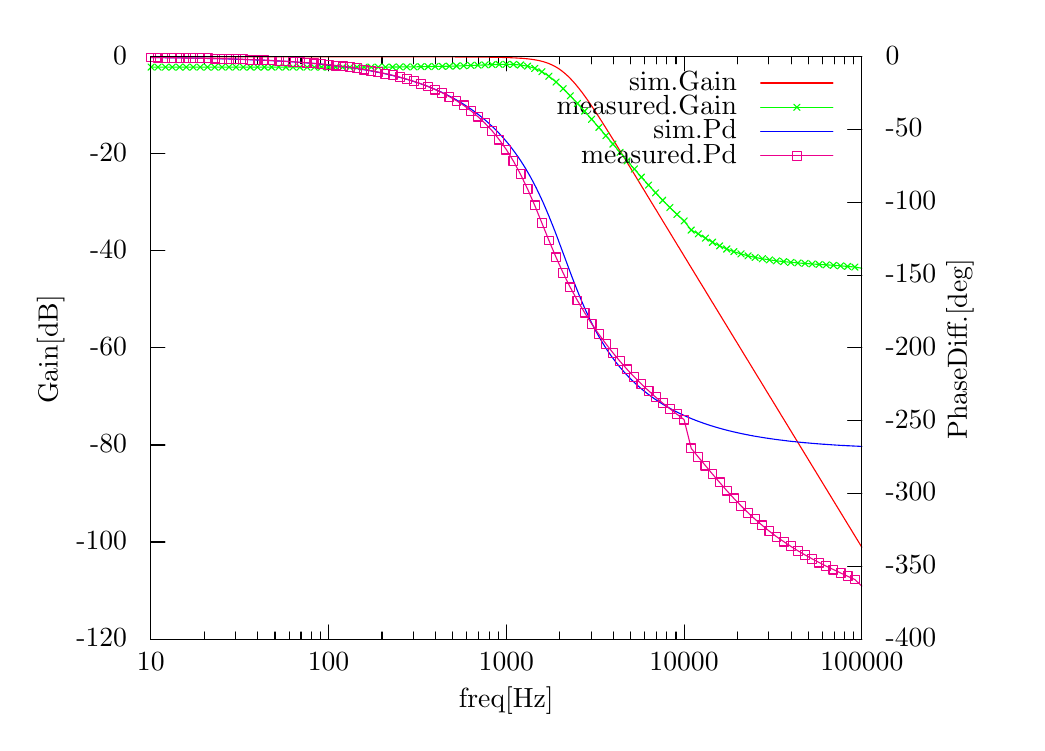
\begin{tikzpicture}[gnuplot]
%% generated with GNUPLOT 4.6p4 (Lua 5.1; terminal rev. 99, script rev. 100)
%% 2016年06月18日 10時17分00秒
\path (0.000,0.000) rectangle (12.500,8.750);
\gpcolor{color=gp lt color border}
\gpsetlinetype{gp lt border}
\gpsetlinewidth{1.00}
\draw[gp path] (1.504,0.985)--(1.684,0.985);
\node[gp node right] at (1.320,0.985) {-120};
\draw[gp path] (1.504,2.218)--(1.684,2.218);
\node[gp node right] at (1.320,2.218) {-100};
\draw[gp path] (1.504,3.450)--(1.684,3.450);
\node[gp node right] at (1.320,3.450) {-80};
\draw[gp path] (1.504,4.683)--(1.684,4.683);
\node[gp node right] at (1.320,4.683) {-60};
\draw[gp path] (1.504,5.916)--(1.684,5.916);
\node[gp node right] at (1.320,5.916) {-40};
\draw[gp path] (1.504,7.148)--(1.684,7.148);
\node[gp node right] at (1.320,7.148) {-20};
\draw[gp path] (1.504,8.381)--(1.684,8.381);
\node[gp node right] at (1.320,8.381) { 0};
\draw[gp path] (1.504,0.985)--(1.504,1.165);
\draw[gp path] (1.504,8.381)--(1.504,8.201);
\node[gp node center] at (1.504,0.677) { 10};
\draw[gp path] (2.184,0.985)--(2.184,1.075);
\draw[gp path] (2.184,8.381)--(2.184,8.291);
\draw[gp path] (2.581,0.985)--(2.581,1.075);
\draw[gp path] (2.581,8.381)--(2.581,8.291);
\draw[gp path] (2.863,0.985)--(2.863,1.075);
\draw[gp path] (2.863,8.381)--(2.863,8.291);
\draw[gp path] (3.082,0.985)--(3.082,1.075);
\draw[gp path] (3.082,8.381)--(3.082,8.291);
\draw[gp path] (3.261,0.985)--(3.261,1.075);
\draw[gp path] (3.261,8.381)--(3.261,8.291);
\draw[gp path] (3.412,0.985)--(3.412,1.075);
\draw[gp path] (3.412,8.381)--(3.412,8.291);
\draw[gp path] (3.543,0.985)--(3.543,1.075);
\draw[gp path] (3.543,8.381)--(3.543,8.291);
\draw[gp path] (3.658,0.985)--(3.658,1.075);
\draw[gp path] (3.658,8.381)--(3.658,8.291);
\draw[gp path] (3.762,0.985)--(3.762,1.165);
\draw[gp path] (3.762,8.381)--(3.762,8.201);
\node[gp node center] at (3.762,0.677) { 100};
\draw[gp path] (4.441,0.985)--(4.441,1.075);
\draw[gp path] (4.441,8.381)--(4.441,8.291);
\draw[gp path] (4.839,0.985)--(4.839,1.075);
\draw[gp path] (4.839,8.381)--(4.839,8.291);
\draw[gp path] (5.121,0.985)--(5.121,1.075);
\draw[gp path] (5.121,8.381)--(5.121,8.291);
\draw[gp path] (5.340,0.985)--(5.340,1.075);
\draw[gp path] (5.340,8.381)--(5.340,8.291);
\draw[gp path] (5.519,0.985)--(5.519,1.075);
\draw[gp path] (5.519,8.381)--(5.519,8.291);
\draw[gp path] (5.670,0.985)--(5.670,1.075);
\draw[gp path] (5.670,8.381)--(5.670,8.291);
\draw[gp path] (5.801,0.985)--(5.801,1.075);
\draw[gp path] (5.801,8.381)--(5.801,8.291);
\draw[gp path] (5.916,0.985)--(5.916,1.075);
\draw[gp path] (5.916,8.381)--(5.916,8.291);
\draw[gp path] (6.020,0.985)--(6.020,1.165);
\draw[gp path] (6.020,8.381)--(6.020,8.201);
\node[gp node center] at (6.020,0.677) { 1000};
\draw[gp path] (6.699,0.985)--(6.699,1.075);
\draw[gp path] (6.699,8.381)--(6.699,8.291);
\draw[gp path] (7.097,0.985)--(7.097,1.075);
\draw[gp path] (7.097,8.381)--(7.097,8.291);
\draw[gp path] (7.379,0.985)--(7.379,1.075);
\draw[gp path] (7.379,8.381)--(7.379,8.291);
\draw[gp path] (7.598,0.985)--(7.598,1.075);
\draw[gp path] (7.598,8.381)--(7.598,8.291);
\draw[gp path] (7.776,0.985)--(7.776,1.075);
\draw[gp path] (7.776,8.381)--(7.776,8.291);
\draw[gp path] (7.928,0.985)--(7.928,1.075);
\draw[gp path] (7.928,8.381)--(7.928,8.291);
\draw[gp path] (8.058,0.985)--(8.058,1.075);
\draw[gp path] (8.058,8.381)--(8.058,8.291);
\draw[gp path] (8.174,0.985)--(8.174,1.075);
\draw[gp path] (8.174,8.381)--(8.174,8.291);
\draw[gp path] (8.277,0.985)--(8.277,1.165);
\draw[gp path] (8.277,8.381)--(8.277,8.201);
\node[gp node center] at (8.277,0.677) { 10000};
\draw[gp path] (8.957,0.985)--(8.957,1.075);
\draw[gp path] (8.957,8.381)--(8.957,8.291);
\draw[gp path] (9.354,0.985)--(9.354,1.075);
\draw[gp path] (9.354,8.381)--(9.354,8.291);
\draw[gp path] (9.637,0.985)--(9.637,1.075);
\draw[gp path] (9.637,8.381)--(9.637,8.291);
\draw[gp path] (9.855,0.985)--(9.855,1.075);
\draw[gp path] (9.855,8.381)--(9.855,8.291);
\draw[gp path] (10.034,0.985)--(10.034,1.075);
\draw[gp path] (10.034,8.381)--(10.034,8.291);
\draw[gp path] (10.185,0.985)--(10.185,1.075);
\draw[gp path] (10.185,8.381)--(10.185,8.291);
\draw[gp path] (10.316,0.985)--(10.316,1.075);
\draw[gp path] (10.316,8.381)--(10.316,8.291);
\draw[gp path] (10.432,0.985)--(10.432,1.075);
\draw[gp path] (10.432,8.381)--(10.432,8.291);
\draw[gp path] (10.535,0.985)--(10.535,1.165);
\draw[gp path] (10.535,8.381)--(10.535,8.201);
\node[gp node center] at (10.535,0.677) { 100000};
\draw[gp path] (10.535,0.985)--(10.355,0.985);
\node[gp node left] at (10.719,0.985) {-400};
\draw[gp path] (10.535,1.910)--(10.355,1.910);
\node[gp node left] at (10.719,1.910) {-350};
\draw[gp path] (10.535,2.834)--(10.355,2.834);
\node[gp node left] at (10.719,2.834) {-300};
\draw[gp path] (10.535,3.758)--(10.355,3.758);
\node[gp node left] at (10.719,3.758) {-250};
\draw[gp path] (10.535,4.683)--(10.355,4.683);
\node[gp node left] at (10.719,4.683) {-200};
\draw[gp path] (10.535,5.608)--(10.355,5.608);
\node[gp node left] at (10.719,5.608) {-150};
\draw[gp path] (10.535,6.532)--(10.355,6.532);
\node[gp node left] at (10.719,6.532) {-100};
\draw[gp path] (10.535,7.456)--(10.355,7.456);
\node[gp node left] at (10.719,7.456) {-50};
\draw[gp path] (10.535,8.381)--(10.355,8.381);
\node[gp node left] at (10.719,8.381) { 0};
\draw[gp path] (1.504,8.381)--(1.504,0.985)--(10.535,0.985)--(10.535,8.381)--cycle;
\node[gp node center,rotate=-270] at (0.246,4.683) {Gain[dB]};
\node[gp node center,rotate=-270] at (11.792,4.683) {PhaseDiff.[deg]};
\node[gp node center] at (6.019,0.215) {freq[Hz]};
\node[gp node right] at (9.067,8.047) {sim.Gain};
\gpcolor{color=gp lt color 0}
\gpsetlinetype{gp lt plot 0}
\draw[gp path] (9.251,8.047)--(10.167,8.047);
\draw[gp path] (1.504,8.381)--(1.509,8.381)--(1.513,8.381)--(1.518,8.381)--(1.522,8.381)%
  --(1.527,8.381)--(1.531,8.381)--(1.536,8.381)--(1.540,8.381)--(1.545,8.381)--(1.549,8.381)%
  --(1.554,8.381)--(1.558,8.381)--(1.563,8.381)--(1.567,8.381)--(1.572,8.381)--(1.576,8.381)%
  --(1.581,8.381)--(1.585,8.381)--(1.590,8.381)--(1.594,8.381)--(1.599,8.381)--(1.603,8.381)%
  --(1.608,8.381)--(1.612,8.381)--(1.617,8.381)--(1.621,8.381)--(1.626,8.381)--(1.630,8.381)%
  --(1.635,8.381)--(1.639,8.381)--(1.644,8.381)--(1.648,8.381)--(1.653,8.381)--(1.658,8.381)%
  --(1.662,8.381)--(1.667,8.381)--(1.671,8.381)--(1.676,8.381)--(1.680,8.381)--(1.685,8.381)%
  --(1.689,8.381)--(1.694,8.381)--(1.698,8.381)--(1.703,8.381)--(1.707,8.381)--(1.712,8.381)%
  --(1.716,8.381)--(1.721,8.381)--(1.725,8.381)--(1.730,8.381)--(1.734,8.381)--(1.739,8.381)%
  --(1.743,8.381)--(1.748,8.381)--(1.752,8.381)--(1.757,8.381)--(1.761,8.381)--(1.766,8.381)%
  --(1.770,8.381)--(1.775,8.381)--(1.779,8.381)--(1.784,8.381)--(1.788,8.381)--(1.793,8.381)%
  --(1.798,8.381)--(1.802,8.381)--(1.807,8.381)--(1.811,8.381)--(1.816,8.381)--(1.820,8.381)%
  --(1.825,8.381)--(1.829,8.381)--(1.834,8.381)--(1.838,8.381)--(1.843,8.381)--(1.847,8.381)%
  --(1.852,8.381)--(1.856,8.381)--(1.861,8.381)--(1.865,8.381)--(1.870,8.381)--(1.874,8.381)%
  --(1.879,8.381)--(1.883,8.381)--(1.888,8.381)--(1.892,8.381)--(1.897,8.381)--(1.901,8.381)%
  --(1.906,8.381)--(1.910,8.381)--(1.915,8.381)--(1.919,8.381)--(1.924,8.381)--(1.928,8.381)%
  --(1.933,8.381)--(1.937,8.381)--(1.942,8.381)--(1.947,8.381)--(1.951,8.381)--(1.956,8.381)%
  --(1.960,8.381)--(1.965,8.381)--(1.969,8.381)--(1.974,8.381)--(1.978,8.381)--(1.983,8.381)%
  --(1.987,8.381)--(1.992,8.381)--(1.996,8.381)--(2.001,8.381)--(2.005,8.381)--(2.010,8.381)%
  --(2.014,8.381)--(2.019,8.381)--(2.023,8.381)--(2.028,8.381)--(2.032,8.381)--(2.037,8.381)%
  --(2.041,8.381)--(2.046,8.381)--(2.050,8.381)--(2.055,8.381)--(2.059,8.381)--(2.064,8.381)%
  --(2.068,8.381)--(2.073,8.381)--(2.077,8.381)--(2.082,8.381)--(2.086,8.381)--(2.091,8.381)%
  --(2.096,8.381)--(2.100,8.381)--(2.105,8.381)--(2.109,8.381)--(2.114,8.381)--(2.118,8.381)%
  --(2.123,8.381)--(2.127,8.381)--(2.132,8.381)--(2.136,8.381)--(2.141,8.381)--(2.145,8.381)%
  --(2.150,8.381)--(2.154,8.381)--(2.159,8.381)--(2.163,8.381)--(2.168,8.381)--(2.172,8.381)%
  --(2.177,8.381)--(2.181,8.381)--(2.186,8.381)--(2.190,8.381)--(2.195,8.381)--(2.199,8.381)%
  --(2.204,8.381)--(2.208,8.381)--(2.213,8.381)--(2.217,8.381)--(2.222,8.381)--(2.226,8.381)%
  --(2.231,8.381)--(2.236,8.381)--(2.240,8.381)--(2.245,8.381)--(2.249,8.381)--(2.254,8.381)%
  --(2.258,8.381)--(2.263,8.381)--(2.267,8.381)--(2.272,8.381)--(2.276,8.381)--(2.281,8.381)%
  --(2.285,8.381)--(2.290,8.381)--(2.294,8.381)--(2.299,8.381)--(2.303,8.381)--(2.308,8.381)%
  --(2.312,8.381)--(2.317,8.381)--(2.321,8.381)--(2.326,8.381)--(2.330,8.381)--(2.335,8.381)%
  --(2.339,8.381)--(2.344,8.381)--(2.348,8.381)--(2.353,8.381)--(2.357,8.381)--(2.362,8.381)%
  --(2.366,8.381)--(2.371,8.381)--(2.375,8.381)--(2.380,8.381)--(2.385,8.381)--(2.389,8.381)%
  --(2.394,8.381)--(2.398,8.381)--(2.403,8.381)--(2.407,8.381)--(2.412,8.381)--(2.416,8.381)%
  --(2.421,8.381)--(2.425,8.381)--(2.430,8.381)--(2.434,8.381)--(2.439,8.381)--(2.443,8.381)%
  --(2.448,8.381)--(2.452,8.381)--(2.457,8.381)--(2.461,8.381)--(2.466,8.381)--(2.470,8.381)%
  --(2.475,8.381)--(2.479,8.381)--(2.484,8.381)--(2.488,8.381)--(2.493,8.381)--(2.497,8.381)%
  --(2.502,8.381)--(2.506,8.381)--(2.511,8.381)--(2.515,8.381)--(2.520,8.381)--(2.525,8.381)%
  --(2.529,8.381)--(2.534,8.381)--(2.538,8.381)--(2.543,8.381)--(2.547,8.381)--(2.552,8.381)%
  --(2.556,8.381)--(2.561,8.381)--(2.565,8.381)--(2.570,8.381)--(2.574,8.381)--(2.579,8.381)%
  --(2.583,8.381)--(2.588,8.381)--(2.592,8.381)--(2.597,8.381)--(2.601,8.381)--(2.606,8.381)%
  --(2.610,8.381)--(2.615,8.381)--(2.619,8.381)--(2.624,8.381)--(2.628,8.381)--(2.633,8.381)%
  --(2.637,8.381)--(2.642,8.381)--(2.646,8.381)--(2.651,8.381)--(2.655,8.381)--(2.660,8.381)%
  --(2.664,8.381)--(2.669,8.381)--(2.674,8.381)--(2.678,8.381)--(2.683,8.381)--(2.687,8.381)%
  --(2.692,8.381)--(2.696,8.381)--(2.701,8.381)--(2.705,8.381)--(2.710,8.381)--(2.714,8.381)%
  --(2.719,8.381)--(2.723,8.381)--(2.728,8.381)--(2.732,8.381)--(2.737,8.381)--(2.741,8.381)%
  --(2.746,8.381)--(2.750,8.381)--(2.755,8.381)--(2.759,8.381)--(2.764,8.381)--(2.768,8.381)%
  --(2.773,8.381)--(2.777,8.381)--(2.782,8.381)--(2.786,8.381)--(2.791,8.381)--(2.795,8.381)%
  --(2.800,8.381)--(2.804,8.381)--(2.809,8.381)--(2.813,8.381)--(2.818,8.381)--(2.823,8.381)%
  --(2.827,8.381)--(2.832,8.381)--(2.836,8.381)--(2.841,8.381)--(2.845,8.381)--(2.850,8.381)%
  --(2.854,8.381)--(2.859,8.381)--(2.863,8.381)--(2.868,8.381)--(2.872,8.381)--(2.877,8.381)%
  --(2.881,8.381)--(2.886,8.381)--(2.890,8.381)--(2.895,8.381)--(2.899,8.381)--(2.904,8.381)%
  --(2.908,8.381)--(2.913,8.381)--(2.917,8.381)--(2.922,8.381)--(2.926,8.381)--(2.931,8.381)%
  --(2.935,8.381)--(2.940,8.381)--(2.944,8.381)--(2.949,8.381)--(2.953,8.381)--(2.958,8.381)%
  --(2.963,8.381)--(2.967,8.381)--(2.972,8.381)--(2.976,8.381)--(2.981,8.381)--(2.985,8.381)%
  --(2.990,8.381)--(2.994,8.381)--(2.999,8.381)--(3.003,8.381)--(3.008,8.381)--(3.012,8.381)%
  --(3.017,8.381)--(3.021,8.381)--(3.026,8.381)--(3.030,8.381)--(3.035,8.381)--(3.039,8.381)%
  --(3.044,8.381)--(3.048,8.381)--(3.053,8.381)--(3.057,8.381)--(3.062,8.381)--(3.066,8.381)%
  --(3.071,8.381)--(3.075,8.381)--(3.080,8.381)--(3.084,8.381)--(3.089,8.381)--(3.093,8.381)%
  --(3.098,8.381)--(3.102,8.381)--(3.107,8.381)--(3.112,8.381)--(3.116,8.381)--(3.121,8.381)%
  --(3.125,8.381)--(3.130,8.381)--(3.134,8.381)--(3.139,8.381)--(3.143,8.381)--(3.148,8.381)%
  --(3.152,8.381)--(3.157,8.381)--(3.161,8.381)--(3.166,8.381)--(3.170,8.381)--(3.175,8.381)%
  --(3.179,8.381)--(3.184,8.381)--(3.188,8.381)--(3.193,8.381)--(3.197,8.381)--(3.202,8.381)%
  --(3.206,8.381)--(3.211,8.381)--(3.215,8.381)--(3.220,8.381)--(3.224,8.381)--(3.229,8.381)%
  --(3.233,8.381)--(3.238,8.381)--(3.242,8.381)--(3.247,8.381)--(3.251,8.381)--(3.256,8.381)%
  --(3.261,8.381)--(3.265,8.381)--(3.270,8.381)--(3.274,8.381)--(3.279,8.381)--(3.283,8.381)%
  --(3.288,8.381)--(3.292,8.381)--(3.297,8.381)--(3.301,8.381)--(3.306,8.381)--(3.310,8.381)%
  --(3.315,8.381)--(3.319,8.381)--(3.324,8.381)--(3.328,8.381)--(3.333,8.381)--(3.337,8.381)%
  --(3.342,8.381)--(3.346,8.381)--(3.351,8.381)--(3.355,8.381)--(3.360,8.381)--(3.364,8.381)%
  --(3.369,8.381)--(3.373,8.381)--(3.378,8.381)--(3.382,8.381)--(3.387,8.381)--(3.391,8.381)%
  --(3.396,8.381)--(3.401,8.381)--(3.405,8.381)--(3.410,8.381)--(3.414,8.381)--(3.419,8.381)%
  --(3.423,8.381)--(3.428,8.381)--(3.432,8.381)--(3.437,8.381)--(3.441,8.381)--(3.446,8.381)%
  --(3.450,8.381)--(3.455,8.381)--(3.459,8.381)--(3.464,8.381)--(3.468,8.381)--(3.473,8.381)%
  --(3.477,8.381)--(3.482,8.381)--(3.486,8.381)--(3.491,8.381)--(3.495,8.381)--(3.500,8.381)%
  --(3.504,8.381)--(3.509,8.381)--(3.513,8.381)--(3.518,8.381)--(3.522,8.381)--(3.527,8.381)%
  --(3.531,8.381)--(3.536,8.381)--(3.540,8.381)--(3.545,8.381)--(3.550,8.381)--(3.554,8.381)%
  --(3.559,8.381)--(3.563,8.381)--(3.568,8.381)--(3.572,8.381)--(3.577,8.381)--(3.581,8.381)%
  --(3.586,8.381)--(3.590,8.381)--(3.595,8.381)--(3.599,8.381)--(3.604,8.381)--(3.608,8.381)%
  --(3.613,8.381)--(3.617,8.381)--(3.622,8.381)--(3.626,8.381)--(3.631,8.381)--(3.635,8.381)%
  --(3.640,8.381)--(3.644,8.381)--(3.649,8.381)--(3.653,8.381)--(3.658,8.381)--(3.662,8.381)%
  --(3.667,8.381)--(3.671,8.381)--(3.676,8.381)--(3.680,8.381)--(3.685,8.381)--(3.690,8.381)%
  --(3.694,8.381)--(3.699,8.381)--(3.703,8.381)--(3.708,8.381)--(3.712,8.381)--(3.717,8.381)%
  --(3.721,8.381)--(3.726,8.381)--(3.730,8.381)--(3.735,8.381)--(3.739,8.381)--(3.744,8.381)%
  --(3.748,8.381)--(3.753,8.381)--(3.757,8.381)--(3.762,8.381)--(3.766,8.381)--(3.771,8.381)%
  --(3.775,8.381)--(3.780,8.381)--(3.784,8.381)--(3.789,8.381)--(3.793,8.381)--(3.798,8.381)%
  --(3.802,8.381)--(3.807,8.381)--(3.811,8.381)--(3.816,8.381)--(3.820,8.381)--(3.825,8.381)%
  --(3.829,8.381)--(3.834,8.381)--(3.839,8.381)--(3.843,8.381)--(3.848,8.381)--(3.852,8.381)%
  --(3.857,8.381)--(3.861,8.381)--(3.866,8.381)--(3.870,8.381)--(3.875,8.381)--(3.879,8.381)%
  --(3.884,8.381)--(3.888,8.381)--(3.893,8.381)--(3.897,8.381)--(3.902,8.381)--(3.906,8.381)%
  --(3.911,8.381)--(3.915,8.381)--(3.920,8.381)--(3.924,8.381)--(3.929,8.381)--(3.933,8.381)%
  --(3.938,8.381)--(3.942,8.381)--(3.947,8.381)--(3.951,8.381)--(3.956,8.381)--(3.960,8.381)%
  --(3.965,8.381)--(3.969,8.381)--(3.974,8.381)--(3.978,8.381)--(3.983,8.381)--(3.988,8.381)%
  --(3.992,8.381)--(3.997,8.381)--(4.001,8.381)--(4.006,8.381)--(4.010,8.381)--(4.015,8.381)%
  --(4.019,8.381)--(4.024,8.381)--(4.028,8.381)--(4.033,8.381)--(4.037,8.381)--(4.042,8.381)%
  --(4.046,8.381)--(4.051,8.381)--(4.055,8.381)--(4.060,8.381)--(4.064,8.381)--(4.069,8.381)%
  --(4.073,8.381)--(4.078,8.381)--(4.082,8.381)--(4.087,8.381)--(4.091,8.381)--(4.096,8.381)%
  --(4.100,8.381)--(4.105,8.381)--(4.109,8.381)--(4.114,8.381)--(4.118,8.381)--(4.123,8.381)%
  --(4.128,8.381)--(4.132,8.381)--(4.137,8.381)--(4.141,8.381)--(4.146,8.381)--(4.150,8.381)%
  --(4.155,8.381)--(4.159,8.381)--(4.164,8.381)--(4.168,8.381)--(4.173,8.381)--(4.177,8.381)%
  --(4.182,8.381)--(4.186,8.381)--(4.191,8.381)--(4.195,8.381)--(4.200,8.381)--(4.204,8.381)%
  --(4.209,8.381)--(4.213,8.381)--(4.218,8.381)--(4.222,8.381)--(4.227,8.381)--(4.231,8.381)%
  --(4.236,8.381)--(4.240,8.381)--(4.245,8.381)--(4.249,8.381)--(4.254,8.381)--(4.258,8.381)%
  --(4.263,8.381)--(4.267,8.381)--(4.272,8.381)--(4.277,8.381)--(4.281,8.381)--(4.286,8.381)%
  --(4.290,8.381)--(4.295,8.381)--(4.299,8.381)--(4.304,8.381)--(4.308,8.381)--(4.313,8.381)%
  --(4.317,8.381)--(4.322,8.381)--(4.326,8.381)--(4.331,8.381)--(4.335,8.381)--(4.340,8.381)%
  --(4.344,8.381)--(4.349,8.381)--(4.353,8.381)--(4.358,8.381)--(4.362,8.381)--(4.367,8.381)%
  --(4.371,8.381)--(4.376,8.381)--(4.380,8.381)--(4.385,8.381)--(4.389,8.381)--(4.394,8.381)%
  --(4.398,8.381)--(4.403,8.381)--(4.407,8.381)--(4.412,8.381)--(4.416,8.381)--(4.421,8.381)%
  --(4.426,8.381)--(4.430,8.381)--(4.435,8.381)--(4.439,8.381)--(4.444,8.381)--(4.448,8.381)%
  --(4.453,8.381)--(4.457,8.381)--(4.462,8.381)--(4.466,8.381)--(4.471,8.381)--(4.475,8.381)%
  --(4.480,8.381)--(4.484,8.381)--(4.489,8.381)--(4.493,8.381)--(4.498,8.381)--(4.502,8.381)%
  --(4.507,8.381)--(4.511,8.381)--(4.516,8.381)--(4.520,8.381)--(4.525,8.381)--(4.529,8.381)%
  --(4.534,8.381)--(4.538,8.381)--(4.543,8.381)--(4.547,8.381)--(4.552,8.381)--(4.556,8.381)%
  --(4.561,8.380)--(4.566,8.380)--(4.570,8.380)--(4.575,8.380)--(4.579,8.380)--(4.584,8.380)%
  --(4.588,8.380)--(4.593,8.380)--(4.597,8.380)--(4.602,8.380)--(4.606,8.380)--(4.611,8.380)%
  --(4.615,8.380)--(4.620,8.380)--(4.624,8.380)--(4.629,8.380)--(4.633,8.380)--(4.638,8.380)%
  --(4.642,8.380)--(4.647,8.380)--(4.651,8.380)--(4.656,8.380)--(4.660,8.380)--(4.665,8.380)%
  --(4.669,8.380)--(4.674,8.380)--(4.678,8.380)--(4.683,8.380)--(4.687,8.380)--(4.692,8.380)%
  --(4.696,8.380)--(4.701,8.380)--(4.705,8.380)--(4.710,8.380)--(4.715,8.380)--(4.719,8.380)%
  --(4.724,8.380)--(4.728,8.380)--(4.733,8.380)--(4.737,8.380)--(4.742,8.380)--(4.746,8.380)%
  --(4.751,8.380)--(4.755,8.380)--(4.760,8.380)--(4.764,8.380)--(4.769,8.380)--(4.773,8.380)%
  --(4.778,8.380)--(4.782,8.380)--(4.787,8.380)--(4.791,8.380)--(4.796,8.380)--(4.800,8.380)%
  --(4.805,8.380)--(4.809,8.380)--(4.814,8.380)--(4.818,8.380)--(4.823,8.380)--(4.827,8.380)%
  --(4.832,8.380)--(4.836,8.380)--(4.841,8.380)--(4.845,8.380)--(4.850,8.380)--(4.855,8.380)%
  --(4.859,8.380)--(4.864,8.380)--(4.868,8.380)--(4.873,8.380)--(4.877,8.380)--(4.882,8.380)%
  --(4.886,8.380)--(4.891,8.380)--(4.895,8.380)--(4.900,8.380)--(4.904,8.380)--(4.909,8.380)%
  --(4.913,8.380)--(4.918,8.380)--(4.922,8.380)--(4.927,8.380)--(4.931,8.380)--(4.936,8.380)%
  --(4.940,8.380)--(4.945,8.380)--(4.949,8.380)--(4.954,8.380)--(4.958,8.380)--(4.963,8.380)%
  --(4.967,8.380)--(4.972,8.380)--(4.976,8.380)--(4.981,8.380)--(4.985,8.380)--(4.990,8.380)%
  --(4.994,8.380)--(4.999,8.380)--(5.004,8.380)--(5.008,8.380)--(5.013,8.380)--(5.017,8.380)%
  --(5.022,8.380)--(5.026,8.380)--(5.031,8.380)--(5.035,8.380)--(5.040,8.380)--(5.044,8.380)%
  --(5.049,8.380)--(5.053,8.380)--(5.058,8.380)--(5.062,8.380)--(5.067,8.380)--(5.071,8.380)%
  --(5.076,8.380)--(5.080,8.380)--(5.085,8.380)--(5.089,8.380)--(5.094,8.380)--(5.098,8.380)%
  --(5.103,8.380)--(5.107,8.380)--(5.112,8.379)--(5.116,8.379)--(5.121,8.379)--(5.125,8.379)%
  --(5.130,8.379)--(5.134,8.379)--(5.139,8.379)--(5.143,8.379)--(5.148,8.379)--(5.153,8.379)%
  --(5.157,8.379)--(5.162,8.379)--(5.166,8.379)--(5.171,8.379)--(5.175,8.379)--(5.180,8.379)%
  --(5.184,8.379)--(5.189,8.379)--(5.193,8.379)--(5.198,8.379)--(5.202,8.379)--(5.207,8.379)%
  --(5.211,8.379)--(5.216,8.379)--(5.220,8.379)--(5.225,8.379)--(5.229,8.379)--(5.234,8.379)%
  --(5.238,8.379)--(5.243,8.379)--(5.247,8.379)--(5.252,8.379)--(5.256,8.379)--(5.261,8.379)%
  --(5.265,8.379)--(5.270,8.379)--(5.274,8.379)--(5.279,8.379)--(5.283,8.379)--(5.288,8.379)%
  --(5.293,8.379)--(5.297,8.379)--(5.302,8.379)--(5.306,8.379)--(5.311,8.379)--(5.315,8.379)%
  --(5.320,8.379)--(5.324,8.379)--(5.329,8.379)--(5.333,8.379)--(5.338,8.379)--(5.342,8.379)%
  --(5.347,8.379)--(5.351,8.379)--(5.356,8.379)--(5.360,8.379)--(5.365,8.379)--(5.369,8.378)%
  --(5.374,8.378)--(5.378,8.378)--(5.383,8.378)--(5.387,8.378)--(5.392,8.378)--(5.396,8.378)%
  --(5.401,8.378)--(5.405,8.378)--(5.410,8.378)--(5.414,8.378)--(5.419,8.378)--(5.423,8.378)%
  --(5.428,8.378)--(5.432,8.378)--(5.437,8.378)--(5.442,8.378)--(5.446,8.378)--(5.451,8.378)%
  --(5.455,8.378)--(5.460,8.378)--(5.464,8.378)--(5.469,8.378)--(5.473,8.378)--(5.478,8.378)%
  --(5.482,8.378)--(5.487,8.378)--(5.491,8.378)--(5.496,8.378)--(5.500,8.378)--(5.505,8.378)%
  --(5.509,8.378)--(5.514,8.378)--(5.518,8.378)--(5.523,8.378)--(5.527,8.378)--(5.532,8.378)%
  --(5.536,8.377)--(5.541,8.377)--(5.545,8.377)--(5.550,8.377)--(5.554,8.377)--(5.559,8.377)%
  --(5.563,8.377)--(5.568,8.377)--(5.572,8.377)--(5.577,8.377)--(5.581,8.377)--(5.586,8.377)%
  --(5.591,8.377)--(5.595,8.377)--(5.600,8.377)--(5.604,8.377)--(5.609,8.377)--(5.613,8.377)%
  --(5.618,8.377)--(5.622,8.377)--(5.627,8.377)--(5.631,8.377)--(5.636,8.377)--(5.640,8.377)%
  --(5.645,8.377)--(5.649,8.377)--(5.654,8.376)--(5.658,8.376)--(5.663,8.376)--(5.667,8.376)%
  --(5.672,8.376)--(5.676,8.376)--(5.681,8.376)--(5.685,8.376)--(5.690,8.376)--(5.694,8.376)%
  --(5.699,8.376)--(5.703,8.376)--(5.708,8.376)--(5.712,8.376)--(5.717,8.376)--(5.721,8.376)%
  --(5.726,8.376)--(5.731,8.376)--(5.735,8.376)--(5.740,8.376)--(5.744,8.376)--(5.749,8.375)%
  --(5.753,8.375)--(5.758,8.375)--(5.762,8.375)--(5.767,8.375)--(5.771,8.375)--(5.776,8.375)%
  --(5.780,8.375)--(5.785,8.375)--(5.789,8.375)--(5.794,8.375)--(5.798,8.375)--(5.803,8.375)%
  --(5.807,8.375)--(5.812,8.375)--(5.816,8.375)--(5.821,8.374)--(5.825,8.374)--(5.830,8.374)%
  --(5.834,8.374)--(5.839,8.374)--(5.843,8.374)--(5.848,8.374)--(5.852,8.374)--(5.857,8.374)%
  --(5.861,8.374)--(5.866,8.374)--(5.870,8.374)--(5.875,8.374)--(5.880,8.374)--(5.884,8.373)%
  --(5.889,8.373)--(5.893,8.373)--(5.898,8.373)--(5.902,8.373)--(5.907,8.373)--(5.911,8.373)%
  --(5.916,8.373)--(5.920,8.373)--(5.925,8.373)--(5.929,8.373)--(5.934,8.372)--(5.938,8.372)%
  --(5.943,8.372)--(5.947,8.372)--(5.952,8.372)--(5.956,8.372)--(5.961,8.372)--(5.965,8.372)%
  --(5.970,8.372)--(5.974,8.371)--(5.979,8.371)--(5.983,8.371)--(5.988,8.371)--(5.992,8.371)%
  --(5.997,8.371)--(6.001,8.371)--(6.006,8.371)--(6.010,8.370)--(6.015,8.370)--(6.020,8.370)%
  --(6.024,8.370)--(6.029,8.370)--(6.033,8.370)--(6.038,8.370)--(6.042,8.369)--(6.047,8.369)%
  --(6.051,8.369)--(6.056,8.369)--(6.060,8.369)--(6.065,8.369)--(6.069,8.369)--(6.074,8.368)%
  --(6.078,8.368)--(6.083,8.368)--(6.087,8.368)--(6.092,8.368)--(6.096,8.367)--(6.101,8.367)%
  --(6.105,8.367)--(6.110,8.367)--(6.114,8.367)--(6.119,8.366)--(6.123,8.366)--(6.128,8.366)%
  --(6.132,8.366)--(6.137,8.366)--(6.141,8.365)--(6.146,8.365)--(6.150,8.365)--(6.155,8.365)%
  --(6.159,8.364)--(6.164,8.364)--(6.169,8.364)--(6.173,8.364)--(6.178,8.363)--(6.182,8.363)%
  --(6.187,8.363)--(6.191,8.362)--(6.196,8.362)--(6.200,8.362)--(6.205,8.362)--(6.209,8.361)%
  --(6.214,8.361)--(6.218,8.361)--(6.223,8.360)--(6.227,8.360)--(6.232,8.360)--(6.236,8.359)%
  --(6.241,8.359)--(6.245,8.358)--(6.250,8.358)--(6.254,8.358)--(6.259,8.357)--(6.263,8.357)%
  --(6.268,8.356)--(6.272,8.356)--(6.277,8.355)--(6.281,8.355)--(6.286,8.355)--(6.290,8.354)%
  --(6.295,8.354)--(6.299,8.353)--(6.304,8.353)--(6.308,8.352)--(6.313,8.352)--(6.318,8.351)%
  --(6.322,8.350)--(6.327,8.350)--(6.331,8.349)--(6.336,8.349)--(6.340,8.348)--(6.345,8.348)%
  --(6.349,8.347)--(6.354,8.346)--(6.358,8.346)--(6.363,8.345)--(6.367,8.344)--(6.372,8.343)%
  --(6.376,8.343)--(6.381,8.342)--(6.385,8.341)--(6.390,8.340)--(6.394,8.340)--(6.399,8.339)%
  --(6.403,8.338)--(6.408,8.337)--(6.412,8.336)--(6.417,8.335)--(6.421,8.334)--(6.426,8.334)%
  --(6.430,8.333)--(6.435,8.332)--(6.439,8.331)--(6.444,8.330)--(6.448,8.329)--(6.453,8.328)%
  --(6.458,8.326)--(6.462,8.325)--(6.467,8.324)--(6.471,8.323)--(6.476,8.322)--(6.480,8.321)%
  --(6.485,8.319)--(6.489,8.318)--(6.494,8.317)--(6.498,8.315)--(6.503,8.314)--(6.507,8.313)%
  --(6.512,8.311)--(6.516,8.310)--(6.521,8.308)--(6.525,8.307)--(6.530,8.305)--(6.534,8.304)%
  --(6.539,8.302)--(6.543,8.300)--(6.548,8.299)--(6.552,8.297)--(6.557,8.295)--(6.561,8.294)%
  --(6.566,8.292)--(6.570,8.290)--(6.575,8.288)--(6.579,8.286)--(6.584,8.284)--(6.588,8.282)%
  --(6.593,8.280)--(6.597,8.278)--(6.602,8.276)--(6.607,8.274)--(6.611,8.271)--(6.616,8.269)%
  --(6.620,8.267)--(6.625,8.264)--(6.629,8.262)--(6.634,8.260)--(6.638,8.257)--(6.643,8.255)%
  --(6.647,8.252)--(6.652,8.249)--(6.656,8.247)--(6.661,8.244)--(6.665,8.241)--(6.670,8.239)%
  --(6.674,8.236)--(6.679,8.233)--(6.683,8.230)--(6.688,8.227)--(6.692,8.224)--(6.697,8.221)%
  --(6.701,8.218)--(6.706,8.214)--(6.710,8.211)--(6.715,8.208)--(6.719,8.204)--(6.724,8.201)%
  --(6.728,8.198)--(6.733,8.194)--(6.737,8.191)--(6.742,8.187)--(6.746,8.183)--(6.751,8.180)%
  --(6.756,8.176)--(6.760,8.172)--(6.765,8.168)--(6.769,8.164)--(6.774,8.160)--(6.778,8.156)%
  --(6.783,8.152)--(6.787,8.148)--(6.792,8.144)--(6.796,8.140)--(6.801,8.136)--(6.805,8.131)%
  --(6.810,8.127)--(6.814,8.123)--(6.819,8.118)--(6.823,8.114)--(6.828,8.109)--(6.832,8.104)%
  --(6.837,8.100)--(6.841,8.095)--(6.846,8.090)--(6.850,8.085)--(6.855,8.081)--(6.859,8.076)%
  --(6.864,8.071)--(6.868,8.066)--(6.873,8.061)--(6.877,8.056)--(6.882,8.051)--(6.886,8.045)%
  --(6.891,8.040)--(6.896,8.035)--(6.900,8.030)--(6.905,8.024)--(6.909,8.019)--(6.914,8.014)%
  --(6.918,8.008)--(6.923,8.003)--(6.927,7.997)--(6.932,7.991)--(6.936,7.986)--(6.941,7.980)%
  --(6.945,7.974)--(6.950,7.969)--(6.954,7.963)--(6.959,7.957)--(6.963,7.951)--(6.968,7.945)%
  --(6.972,7.940)--(6.977,7.934)--(6.981,7.928)--(6.986,7.922)--(6.990,7.916)--(6.995,7.910)%
  --(6.999,7.903)--(7.004,7.897)--(7.008,7.891)--(7.013,7.885)--(7.017,7.879)--(7.022,7.872)%
  --(7.026,7.866)--(7.031,7.860)--(7.035,7.854)--(7.040,7.847)--(7.045,7.841)--(7.049,7.834)%
  --(7.054,7.828)--(7.058,7.821)--(7.063,7.815)--(7.067,7.808)--(7.072,7.802)--(7.076,7.795)%
  --(7.081,7.789)--(7.085,7.782)--(7.090,7.776)--(7.094,7.769)--(7.099,7.762)--(7.103,7.756)%
  --(7.108,7.749)--(7.112,7.742)--(7.117,7.735)--(7.121,7.729)--(7.126,7.722)--(7.130,7.715)%
  --(7.135,7.708)--(7.139,7.701)--(7.144,7.695)--(7.148,7.688)--(7.153,7.681)--(7.157,7.674)%
  --(7.162,7.667)--(7.166,7.660)--(7.171,7.653)--(7.175,7.646)--(7.180,7.639)--(7.184,7.632)%
  --(7.189,7.625)--(7.194,7.618)--(7.198,7.611)--(7.203,7.604)--(7.207,7.597)--(7.212,7.590)%
  --(7.216,7.583)--(7.221,7.576)--(7.225,7.569)--(7.230,7.562)--(7.234,7.555)--(7.239,7.548)%
  --(7.243,7.541)--(7.248,7.534)--(7.252,7.527)--(7.257,7.519)--(7.261,7.512)--(7.266,7.505)%
  --(7.270,7.498)--(7.275,7.491)--(7.279,7.484)--(7.284,7.476)--(7.288,7.469)--(7.293,7.462)%
  --(7.297,7.455)--(7.302,7.448)--(7.306,7.440)--(7.311,7.433)--(7.315,7.426)--(7.320,7.419)%
  --(7.324,7.411)--(7.329,7.404)--(7.334,7.397)--(7.338,7.390)--(7.343,7.382)--(7.347,7.375)%
  --(7.352,7.368)--(7.356,7.361)--(7.361,7.353)--(7.365,7.346)--(7.370,7.339)--(7.374,7.332)%
  --(7.379,7.324)--(7.383,7.317)--(7.388,7.310)--(7.392,7.302)--(7.397,7.295)--(7.401,7.288)%
  --(7.406,7.280)--(7.410,7.273)--(7.415,7.266)--(7.419,7.258)--(7.424,7.251)--(7.428,7.244)%
  --(7.433,7.236)--(7.437,7.229)--(7.442,7.222)--(7.446,7.214)--(7.451,7.207)--(7.455,7.200)%
  --(7.460,7.192)--(7.464,7.185)--(7.469,7.178)--(7.473,7.170)--(7.478,7.163)--(7.483,7.155)%
  --(7.487,7.148)--(7.492,7.141)--(7.496,7.133)--(7.501,7.126)--(7.505,7.119)--(7.510,7.111)%
  --(7.514,7.104)--(7.519,7.096)--(7.523,7.089)--(7.528,7.082)--(7.532,7.074)--(7.537,7.067)%
  --(7.541,7.060)--(7.546,7.052)--(7.550,7.045)--(7.555,7.037)--(7.559,7.030)--(7.564,7.023)%
  --(7.568,7.015)--(7.573,7.008)--(7.577,7.000)--(7.582,6.993)--(7.586,6.986)--(7.591,6.978)%
  --(7.595,6.971)--(7.600,6.963)--(7.604,6.956)--(7.609,6.949)--(7.613,6.941)--(7.618,6.934)%
  --(7.623,6.926)--(7.627,6.919)--(7.632,6.912)--(7.636,6.904)--(7.641,6.897)--(7.645,6.889)%
  --(7.650,6.882)--(7.654,6.874)--(7.659,6.867)--(7.663,6.860)--(7.668,6.852)--(7.672,6.845)%
  --(7.677,6.837)--(7.681,6.830)--(7.686,6.823)--(7.690,6.815)--(7.695,6.808)--(7.699,6.800)%
  --(7.704,6.793)--(7.708,6.786)--(7.713,6.778)--(7.717,6.771)--(7.722,6.763)--(7.726,6.756)%
  --(7.731,6.748)--(7.735,6.741)--(7.740,6.734)--(7.744,6.726)--(7.749,6.719)--(7.753,6.711)%
  --(7.758,6.704)--(7.762,6.697)--(7.767,6.689)--(7.772,6.682)--(7.776,6.674)--(7.781,6.667)%
  --(7.785,6.659)--(7.790,6.652)--(7.794,6.645)--(7.799,6.637)--(7.803,6.630)--(7.808,6.622)%
  --(7.812,6.615)--(7.817,6.607)--(7.821,6.600)--(7.826,6.593)--(7.830,6.585)--(7.835,6.578)%
  --(7.839,6.570)--(7.844,6.563)--(7.848,6.556)--(7.853,6.548)--(7.857,6.541)--(7.862,6.533)%
  --(7.866,6.526)--(7.871,6.518)--(7.875,6.511)--(7.880,6.504)--(7.884,6.496)--(7.889,6.489)%
  --(7.893,6.481)--(7.898,6.474)--(7.902,6.467)--(7.907,6.459)--(7.911,6.452)--(7.916,6.444)%
  --(7.921,6.437)--(7.925,6.429)--(7.930,6.422)--(7.934,6.415)--(7.939,6.407)--(7.943,6.400)%
  --(7.948,6.392)--(7.952,6.385)--(7.957,6.377)--(7.961,6.370)--(7.966,6.363)--(7.970,6.355)%
  --(7.975,6.348)--(7.979,6.340)--(7.984,6.333)--(7.988,6.326)--(7.993,6.318)--(7.997,6.311)%
  --(8.002,6.303)--(8.006,6.296)--(8.011,6.288)--(8.015,6.281)--(8.020,6.274)--(8.024,6.266)%
  --(8.029,6.259)--(8.033,6.251)--(8.038,6.244)--(8.042,6.237)--(8.047,6.229)--(8.051,6.222)%
  --(8.056,6.214)--(8.061,6.207)--(8.065,6.199)--(8.070,6.192)--(8.074,6.185)--(8.079,6.177)%
  --(8.083,6.170)--(8.088,6.162)--(8.092,6.155)--(8.097,6.148)--(8.101,6.140)--(8.106,6.133)%
  --(8.110,6.125)--(8.115,6.118)--(8.119,6.110)--(8.124,6.103)--(8.128,6.096)--(8.133,6.088)%
  --(8.137,6.081)--(8.142,6.073)--(8.146,6.066)--(8.151,6.059)--(8.155,6.051)--(8.160,6.044)%
  --(8.164,6.036)--(8.169,6.029)--(8.173,6.022)--(8.178,6.014)--(8.182,6.007)--(8.187,5.999)%
  --(8.191,5.992)--(8.196,5.984)--(8.200,5.977)--(8.205,5.970)--(8.210,5.962)--(8.214,5.955)%
  --(8.219,5.947)--(8.223,5.940)--(8.228,5.933)--(8.232,5.925)--(8.237,5.918)--(8.241,5.910)%
  --(8.246,5.903)--(8.250,5.896)--(8.255,5.888)--(8.259,5.881)--(8.264,5.873)--(8.268,5.866)%
  --(8.273,5.858)--(8.277,5.851)--(8.282,5.844)--(8.286,5.836)--(8.291,5.829)--(8.295,5.821)%
  --(8.300,5.814)--(8.304,5.807)--(8.309,5.799)--(8.313,5.792)--(8.318,5.784)--(8.322,5.777)%
  --(8.327,5.770)--(8.331,5.762)--(8.336,5.755)--(8.340,5.747)--(8.345,5.740)--(8.349,5.732)%
  --(8.354,5.725)--(8.359,5.718)--(8.363,5.710)--(8.368,5.703)--(8.372,5.695)--(8.377,5.688)%
  --(8.381,5.681)--(8.386,5.673)--(8.390,5.666)--(8.395,5.658)--(8.399,5.651)--(8.404,5.644)%
  --(8.408,5.636)--(8.413,5.629)--(8.417,5.621)--(8.422,5.614)--(8.426,5.607)--(8.431,5.599)%
  --(8.435,5.592)--(8.440,5.584)--(8.444,5.577)--(8.449,5.570)--(8.453,5.562)--(8.458,5.555)%
  --(8.462,5.547)--(8.467,5.540)--(8.471,5.532)--(8.476,5.525)--(8.480,5.518)--(8.485,5.510)%
  --(8.489,5.503)--(8.494,5.495)--(8.499,5.488)--(8.503,5.481)--(8.508,5.473)--(8.512,5.466)%
  --(8.517,5.458)--(8.521,5.451)--(8.526,5.444)--(8.530,5.436)--(8.535,5.429)--(8.539,5.421)%
  --(8.544,5.414)--(8.548,5.407)--(8.553,5.399)--(8.557,5.392)--(8.562,5.384)--(8.566,5.377)%
  --(8.571,5.370)--(8.575,5.362)--(8.580,5.355)--(8.584,5.347)--(8.589,5.340)--(8.593,5.333)%
  --(8.598,5.325)--(8.602,5.318)--(8.607,5.310)--(8.611,5.303)--(8.616,5.296)--(8.620,5.288)%
  --(8.625,5.281)--(8.629,5.273)--(8.634,5.266)--(8.638,5.259)--(8.643,5.251)--(8.648,5.244)%
  --(8.652,5.236)--(8.657,5.229)--(8.661,5.221)--(8.666,5.214)--(8.670,5.207)--(8.675,5.199)%
  --(8.679,5.192)--(8.684,5.184)--(8.688,5.177)--(8.693,5.170)--(8.697,5.162)--(8.702,5.155)%
  --(8.706,5.147)--(8.711,5.140)--(8.715,5.133)--(8.720,5.125)--(8.724,5.118)--(8.729,5.110)%
  --(8.733,5.103)--(8.738,5.096)--(8.742,5.088)--(8.747,5.081)--(8.751,5.073)--(8.756,5.066)%
  --(8.760,5.059)--(8.765,5.051)--(8.769,5.044)--(8.774,5.036)--(8.778,5.029)--(8.783,5.022)%
  --(8.788,5.014)--(8.792,5.007)--(8.797,4.999)--(8.801,4.992)--(8.806,4.985)--(8.810,4.977)%
  --(8.815,4.970)--(8.819,4.962)--(8.824,4.955)--(8.828,4.948)--(8.833,4.940)--(8.837,4.933)%
  --(8.842,4.925)--(8.846,4.918)--(8.851,4.911)--(8.855,4.903)--(8.860,4.896)--(8.864,4.888)%
  --(8.869,4.881)--(8.873,4.874)--(8.878,4.866)--(8.882,4.859)--(8.887,4.851)--(8.891,4.844)%
  --(8.896,4.837)--(8.900,4.829)--(8.905,4.822)--(8.909,4.814)--(8.914,4.807)--(8.918,4.800)%
  --(8.923,4.792)--(8.927,4.785)--(8.932,4.777)--(8.937,4.770)--(8.941,4.763)--(8.946,4.755)%
  --(8.950,4.748)--(8.955,4.740)--(8.959,4.733)--(8.964,4.726)--(8.968,4.718)--(8.973,4.711)%
  --(8.977,4.703)--(8.982,4.696)--(8.986,4.689)--(8.991,4.681)--(8.995,4.674)--(9.000,4.666)%
  --(9.004,4.659)--(9.009,4.652)--(9.013,4.644)--(9.018,4.637)--(9.022,4.629)--(9.027,4.622)%
  --(9.031,4.615)--(9.036,4.607)--(9.040,4.600)--(9.045,4.592)--(9.049,4.585)--(9.054,4.578)%
  --(9.058,4.570)--(9.063,4.563)--(9.067,4.555)--(9.072,4.548)--(9.076,4.541)--(9.081,4.533)%
  --(9.086,4.526)--(9.090,4.518)--(9.095,4.511)--(9.099,4.504)--(9.104,4.496)--(9.108,4.489)%
  --(9.113,4.481)--(9.117,4.474)--(9.122,4.467)--(9.126,4.459)--(9.131,4.452)--(9.135,4.444)%
  --(9.140,4.437)--(9.144,4.430)--(9.149,4.422)--(9.153,4.415)--(9.158,4.407)--(9.162,4.400)%
  --(9.167,4.393)--(9.171,4.385)--(9.176,4.378)--(9.180,4.370)--(9.185,4.363)--(9.189,4.356)%
  --(9.194,4.348)--(9.198,4.341)--(9.203,4.333)--(9.207,4.326)--(9.212,4.319)--(9.216,4.311)%
  --(9.221,4.304)--(9.226,4.296)--(9.230,4.289)--(9.235,4.282)--(9.239,4.274)--(9.244,4.267)%
  --(9.248,4.259)--(9.253,4.252)--(9.257,4.245)--(9.262,4.237)--(9.266,4.230)--(9.271,4.222)%
  --(9.275,4.215)--(9.280,4.208)--(9.284,4.200)--(9.289,4.193)--(9.293,4.185)--(9.298,4.178)%
  --(9.302,4.171)--(9.307,4.163)--(9.311,4.156)--(9.316,4.148)--(9.320,4.141)--(9.325,4.134)%
  --(9.329,4.126)--(9.334,4.119)--(9.338,4.112)--(9.343,4.104)--(9.347,4.097)--(9.352,4.089)%
  --(9.356,4.082)--(9.361,4.075)--(9.365,4.067)--(9.370,4.060)--(9.375,4.052)--(9.379,4.045)%
  --(9.384,4.038)--(9.388,4.030)--(9.393,4.023)--(9.397,4.015)--(9.402,4.008)--(9.406,4.001)%
  --(9.411,3.993)--(9.415,3.986)--(9.420,3.978)--(9.424,3.971)--(9.429,3.964)--(9.433,3.956)%
  --(9.438,3.949)--(9.442,3.941)--(9.447,3.934)--(9.451,3.927)--(9.456,3.919)--(9.460,3.912)%
  --(9.465,3.904)--(9.469,3.897)--(9.474,3.890)--(9.478,3.882)--(9.483,3.875)--(9.487,3.867)%
  --(9.492,3.860)--(9.496,3.853)--(9.501,3.845)--(9.505,3.838)--(9.510,3.830)--(9.514,3.823)%
  --(9.519,3.816)--(9.524,3.808)--(9.528,3.801)--(9.533,3.793)--(9.537,3.786)--(9.542,3.779)%
  --(9.546,3.771)--(9.551,3.764)--(9.555,3.756)--(9.560,3.749)--(9.564,3.742)--(9.569,3.734)%
  --(9.573,3.727)--(9.578,3.719)--(9.582,3.712)--(9.587,3.705)--(9.591,3.697)--(9.596,3.690)%
  --(9.600,3.682)--(9.605,3.675)--(9.609,3.668)--(9.614,3.660)--(9.618,3.653)--(9.623,3.645)%
  --(9.627,3.638)--(9.632,3.631)--(9.636,3.623)--(9.641,3.616)--(9.645,3.608)--(9.650,3.601)%
  --(9.654,3.594)--(9.659,3.586)--(9.664,3.579)--(9.668,3.571)--(9.673,3.564)--(9.677,3.557)%
  --(9.682,3.549)--(9.686,3.542)--(9.691,3.535)--(9.695,3.527)--(9.700,3.520)--(9.704,3.512)%
  --(9.709,3.505)--(9.713,3.498)--(9.718,3.490)--(9.722,3.483)--(9.727,3.475)--(9.731,3.468)%
  --(9.736,3.461)--(9.740,3.453)--(9.745,3.446)--(9.749,3.438)--(9.754,3.431)--(9.758,3.424)%
  --(9.763,3.416)--(9.767,3.409)--(9.772,3.401)--(9.776,3.394)--(9.781,3.387)--(9.785,3.379)%
  --(9.790,3.372)--(9.794,3.364)--(9.799,3.357)--(9.803,3.350)--(9.808,3.342)--(9.813,3.335)%
  --(9.817,3.327)--(9.822,3.320)--(9.826,3.313)--(9.831,3.305)--(9.835,3.298)--(9.840,3.290)%
  --(9.844,3.283)--(9.849,3.276)--(9.853,3.268)--(9.858,3.261)--(9.862,3.253)--(9.867,3.246)%
  --(9.871,3.239)--(9.876,3.231)--(9.880,3.224)--(9.885,3.216)--(9.889,3.209)--(9.894,3.202)%
  --(9.898,3.194)--(9.903,3.187)--(9.907,3.179)--(9.912,3.172)--(9.916,3.165)--(9.921,3.157)%
  --(9.925,3.150)--(9.930,3.142)--(9.934,3.135)--(9.939,3.128)--(9.943,3.120)--(9.948,3.113)%
  --(9.953,3.106)--(9.957,3.098)--(9.962,3.091)--(9.966,3.083)--(9.971,3.076)--(9.975,3.069)%
  --(9.980,3.061)--(9.984,3.054)--(9.989,3.046)--(9.993,3.039)--(9.998,3.032)--(10.002,3.024)%
  --(10.007,3.017)--(10.011,3.009)--(10.016,3.002)--(10.020,2.995)--(10.025,2.987)--(10.029,2.980)%
  --(10.034,2.972)--(10.038,2.965)--(10.043,2.958)--(10.047,2.950)--(10.052,2.943)--(10.056,2.935)%
  --(10.061,2.928)--(10.065,2.921)--(10.070,2.913)--(10.074,2.906)--(10.079,2.898)--(10.083,2.891)%
  --(10.088,2.884)--(10.092,2.876)--(10.097,2.869)--(10.102,2.861)--(10.106,2.854)--(10.111,2.847)%
  --(10.115,2.839)--(10.120,2.832)--(10.124,2.824)--(10.129,2.817)--(10.133,2.810)--(10.138,2.802)%
  --(10.142,2.795)--(10.147,2.787)--(10.151,2.780)--(10.156,2.773)--(10.160,2.765)--(10.165,2.758)%
  --(10.169,2.750)--(10.174,2.743)--(10.178,2.736)--(10.183,2.728)--(10.187,2.721)--(10.192,2.713)%
  --(10.196,2.706)--(10.201,2.699)--(10.205,2.691)--(10.210,2.684)--(10.214,2.677)--(10.219,2.669)%
  --(10.223,2.662)--(10.228,2.654)--(10.232,2.647)--(10.237,2.640)--(10.241,2.632)--(10.246,2.625)%
  --(10.251,2.617)--(10.255,2.610)--(10.260,2.603)--(10.264,2.595)--(10.269,2.588)--(10.273,2.580)%
  --(10.278,2.573)--(10.282,2.566)--(10.287,2.558)--(10.291,2.551)--(10.296,2.543)--(10.300,2.536)%
  --(10.305,2.529)--(10.309,2.521)--(10.314,2.514)--(10.318,2.506)--(10.323,2.499)--(10.327,2.492)%
  --(10.332,2.484)--(10.336,2.477)--(10.341,2.469)--(10.345,2.462)--(10.350,2.455)--(10.354,2.447)%
  --(10.359,2.440)--(10.363,2.432)--(10.368,2.425)--(10.372,2.418)--(10.377,2.410)--(10.381,2.403)%
  --(10.386,2.395)--(10.391,2.388)--(10.395,2.381)--(10.400,2.373)--(10.404,2.366)--(10.409,2.358)%
  --(10.413,2.351)--(10.418,2.344)--(10.422,2.336)--(10.427,2.329)--(10.431,2.321)--(10.436,2.314)%
  --(10.440,2.307)--(10.445,2.299)--(10.449,2.292)--(10.454,2.285)--(10.458,2.277)--(10.463,2.270)%
  --(10.467,2.262)--(10.472,2.255)--(10.476,2.248)--(10.481,2.240)--(10.485,2.233)--(10.490,2.225)%
  --(10.494,2.218)--(10.499,2.211)--(10.503,2.203)--(10.508,2.196)--(10.512,2.188)--(10.517,2.181)%
  --(10.521,2.174)--(10.526,2.166)--(10.530,2.159)--(10.535,2.151);
\gpcolor{color=gp lt color border}
\node[gp node right] at (9.067,7.739) {measured.Gain};
\gpcolor{color=gp lt color 1}
\gpsetlinetype{gp lt plot 1}
\draw[gp path] (9.251,7.739)--(10.167,7.739);
\draw[gp path] (1.510,8.250)--(1.597,8.249)--(1.691,8.249)--(1.778,8.249)--(1.870,8.249)%
  --(1.955,8.249)--(2.043,8.249)--(2.133,8.249)--(2.225,8.249)--(2.317,8.249)--(2.408,8.249)%
  --(2.498,8.249)--(2.587,8.249)--(2.679,8.249)--(2.769,8.249)--(2.860,8.249)--(2.947,8.249)%
  --(3.039,8.249)--(3.130,8.249)--(3.220,8.249)--(3.311,8.249)--(3.399,8.248)--(3.490,8.248)%
  --(3.582,8.248)--(3.672,8.248)--(3.762,8.248)--(3.853,8.248)--(3.942,8.248)--(4.033,8.248)%
  --(4.123,8.248)--(4.213,8.248)--(4.304,8.249)--(4.394,8.249)--(4.485,8.249)--(4.575,8.250)%
  --(4.665,8.251)--(4.755,8.252)--(4.845,8.252)--(4.936,8.254)--(5.026,8.255)--(5.116,8.257)%
  --(5.207,8.259)--(5.297,8.261)--(5.387,8.263)--(5.478,8.266)--(5.568,8.270)--(5.658,8.273)%
  --(5.749,8.277)--(5.839,8.280)--(5.929,8.283)--(6.020,8.285)--(6.110,8.283)--(6.200,8.276)%
  --(6.290,8.261)--(6.381,8.234)--(6.471,8.191)--(6.561,8.133)--(6.652,8.059)--(6.742,7.975)%
  --(6.832,7.884)--(6.923,7.788)--(7.013,7.689)--(7.103,7.587)--(7.194,7.483)--(7.284,7.378)%
  --(7.374,7.272)--(7.464,7.166)--(7.555,7.059)--(7.645,6.955)--(7.735,6.852)--(7.826,6.751)%
  --(7.916,6.653)--(8.006,6.558)--(8.097,6.466)--(8.187,6.379)--(8.277,6.295)--(8.368,6.180)%
  --(8.458,6.131)--(8.548,6.077)--(8.638,6.025)--(8.729,5.979)--(8.819,5.939)--(8.909,5.905)%
  --(9.000,5.877)--(9.090,5.852)--(9.180,5.832)--(9.271,5.815)--(9.361,5.801)--(9.451,5.789)%
  --(9.542,5.779)--(9.632,5.770)--(9.722,5.762)--(9.813,5.756)--(9.903,5.749)--(9.993,5.743)%
  --(10.083,5.738)--(10.174,5.732)--(10.264,5.725)--(10.354,5.718)--(10.445,5.710)--(10.535,5.695);
\gpsetpointsize{4.00}
\gppoint{gp mark 2}{(1.510,8.250)}
\gppoint{gp mark 2}{(1.597,8.249)}
\gppoint{gp mark 2}{(1.691,8.249)}
\gppoint{gp mark 2}{(1.778,8.249)}
\gppoint{gp mark 2}{(1.870,8.249)}
\gppoint{gp mark 2}{(1.955,8.249)}
\gppoint{gp mark 2}{(2.043,8.249)}
\gppoint{gp mark 2}{(2.133,8.249)}
\gppoint{gp mark 2}{(2.225,8.249)}
\gppoint{gp mark 2}{(2.317,8.249)}
\gppoint{gp mark 2}{(2.408,8.249)}
\gppoint{gp mark 2}{(2.498,8.249)}
\gppoint{gp mark 2}{(2.587,8.249)}
\gppoint{gp mark 2}{(2.679,8.249)}
\gppoint{gp mark 2}{(2.769,8.249)}
\gppoint{gp mark 2}{(2.860,8.249)}
\gppoint{gp mark 2}{(2.947,8.249)}
\gppoint{gp mark 2}{(3.039,8.249)}
\gppoint{gp mark 2}{(3.130,8.249)}
\gppoint{gp mark 2}{(3.220,8.249)}
\gppoint{gp mark 2}{(3.311,8.249)}
\gppoint{gp mark 2}{(3.399,8.248)}
\gppoint{gp mark 2}{(3.490,8.248)}
\gppoint{gp mark 2}{(3.582,8.248)}
\gppoint{gp mark 2}{(3.672,8.248)}
\gppoint{gp mark 2}{(3.762,8.248)}
\gppoint{gp mark 2}{(3.853,8.248)}
\gppoint{gp mark 2}{(3.942,8.248)}
\gppoint{gp mark 2}{(4.033,8.248)}
\gppoint{gp mark 2}{(4.123,8.248)}
\gppoint{gp mark 2}{(4.213,8.248)}
\gppoint{gp mark 2}{(4.304,8.249)}
\gppoint{gp mark 2}{(4.394,8.249)}
\gppoint{gp mark 2}{(4.485,8.249)}
\gppoint{gp mark 2}{(4.575,8.250)}
\gppoint{gp mark 2}{(4.665,8.251)}
\gppoint{gp mark 2}{(4.755,8.252)}
\gppoint{gp mark 2}{(4.845,8.252)}
\gppoint{gp mark 2}{(4.936,8.254)}
\gppoint{gp mark 2}{(5.026,8.255)}
\gppoint{gp mark 2}{(5.116,8.257)}
\gppoint{gp mark 2}{(5.207,8.259)}
\gppoint{gp mark 2}{(5.297,8.261)}
\gppoint{gp mark 2}{(5.387,8.263)}
\gppoint{gp mark 2}{(5.478,8.266)}
\gppoint{gp mark 2}{(5.568,8.270)}
\gppoint{gp mark 2}{(5.658,8.273)}
\gppoint{gp mark 2}{(5.749,8.277)}
\gppoint{gp mark 2}{(5.839,8.280)}
\gppoint{gp mark 2}{(5.929,8.283)}
\gppoint{gp mark 2}{(6.020,8.285)}
\gppoint{gp mark 2}{(6.110,8.283)}
\gppoint{gp mark 2}{(6.200,8.276)}
\gppoint{gp mark 2}{(6.290,8.261)}
\gppoint{gp mark 2}{(6.381,8.234)}
\gppoint{gp mark 2}{(6.471,8.191)}
\gppoint{gp mark 2}{(6.561,8.133)}
\gppoint{gp mark 2}{(6.652,8.059)}
\gppoint{gp mark 2}{(6.742,7.975)}
\gppoint{gp mark 2}{(6.832,7.884)}
\gppoint{gp mark 2}{(6.923,7.788)}
\gppoint{gp mark 2}{(7.013,7.689)}
\gppoint{gp mark 2}{(7.103,7.587)}
\gppoint{gp mark 2}{(7.194,7.483)}
\gppoint{gp mark 2}{(7.284,7.378)}
\gppoint{gp mark 2}{(7.374,7.272)}
\gppoint{gp mark 2}{(7.464,7.166)}
\gppoint{gp mark 2}{(7.555,7.059)}
\gppoint{gp mark 2}{(7.645,6.955)}
\gppoint{gp mark 2}{(7.735,6.852)}
\gppoint{gp mark 2}{(7.826,6.751)}
\gppoint{gp mark 2}{(7.916,6.653)}
\gppoint{gp mark 2}{(8.006,6.558)}
\gppoint{gp mark 2}{(8.097,6.466)}
\gppoint{gp mark 2}{(8.187,6.379)}
\gppoint{gp mark 2}{(8.277,6.295)}
\gppoint{gp mark 2}{(8.368,6.180)}
\gppoint{gp mark 2}{(8.458,6.131)}
\gppoint{gp mark 2}{(8.548,6.077)}
\gppoint{gp mark 2}{(8.638,6.025)}
\gppoint{gp mark 2}{(8.729,5.979)}
\gppoint{gp mark 2}{(8.819,5.939)}
\gppoint{gp mark 2}{(8.909,5.905)}
\gppoint{gp mark 2}{(9.000,5.877)}
\gppoint{gp mark 2}{(9.090,5.852)}
\gppoint{gp mark 2}{(9.180,5.832)}
\gppoint{gp mark 2}{(9.271,5.815)}
\gppoint{gp mark 2}{(9.361,5.801)}
\gppoint{gp mark 2}{(9.451,5.789)}
\gppoint{gp mark 2}{(9.542,5.779)}
\gppoint{gp mark 2}{(9.632,5.770)}
\gppoint{gp mark 2}{(9.722,5.762)}
\gppoint{gp mark 2}{(9.813,5.756)}
\gppoint{gp mark 2}{(9.903,5.749)}
\gppoint{gp mark 2}{(9.993,5.743)}
\gppoint{gp mark 2}{(10.083,5.738)}
\gppoint{gp mark 2}{(10.174,5.732)}
\gppoint{gp mark 2}{(10.264,5.725)}
\gppoint{gp mark 2}{(10.354,5.718)}
\gppoint{gp mark 2}{(10.445,5.710)}
\gppoint{gp mark 2}{(9.709,7.739)}
\gpcolor{color=gp lt color border}
\node[gp node right] at (9.067,7.431) {sim.Pd};
\gpcolor{color=gp lt color 2}
\gpsetlinetype{gp lt plot 2}
\draw[gp path] (9.251,7.431)--(10.167,7.431);
\draw[gp path] (1.504,8.371)--(1.509,8.371)--(1.513,8.371)--(1.518,8.370)--(1.522,8.370)%
  --(1.527,8.370)--(1.531,8.370)--(1.536,8.370)--(1.540,8.370)--(1.545,8.370)--(1.549,8.370)%
  --(1.554,8.370)--(1.558,8.370)--(1.563,8.370)--(1.567,8.370)--(1.572,8.370)--(1.576,8.370)%
  --(1.581,8.370)--(1.585,8.370)--(1.590,8.370)--(1.594,8.370)--(1.599,8.370)--(1.603,8.370)%
  --(1.608,8.369)--(1.612,8.369)--(1.617,8.369)--(1.621,8.369)--(1.626,8.369)--(1.630,8.369)%
  --(1.635,8.369)--(1.639,8.369)--(1.644,8.369)--(1.648,8.369)--(1.653,8.369)--(1.658,8.369)%
  --(1.662,8.369)--(1.667,8.369)--(1.671,8.369)--(1.676,8.369)--(1.680,8.369)--(1.685,8.369)%
  --(1.689,8.368)--(1.694,8.368)--(1.698,8.368)--(1.703,8.368)--(1.707,8.368)--(1.712,8.368)%
  --(1.716,8.368)--(1.721,8.368)--(1.725,8.368)--(1.730,8.368)--(1.734,8.368)--(1.739,8.368)%
  --(1.743,8.368)--(1.748,8.368)--(1.752,8.368)--(1.757,8.368)--(1.761,8.367)--(1.766,8.367)%
  --(1.770,8.367)--(1.775,8.367)--(1.779,8.367)--(1.784,8.367)--(1.788,8.367)--(1.793,8.367)%
  --(1.798,8.367)--(1.802,8.367)--(1.807,8.367)--(1.811,8.367)--(1.816,8.367)--(1.820,8.367)%
  --(1.825,8.367)--(1.829,8.367)--(1.834,8.366)--(1.838,8.366)--(1.843,8.366)--(1.847,8.366)%
  --(1.852,8.366)--(1.856,8.366)--(1.861,8.366)--(1.865,8.366)--(1.870,8.366)--(1.874,8.366)%
  --(1.879,8.366)--(1.883,8.366)--(1.888,8.366)--(1.892,8.366)--(1.897,8.365)--(1.901,8.365)%
  --(1.906,8.365)--(1.910,8.365)--(1.915,8.365)--(1.919,8.365)--(1.924,8.365)--(1.928,8.365)%
  --(1.933,8.365)--(1.937,8.365)--(1.942,8.365)--(1.947,8.365)--(1.951,8.365)--(1.956,8.365)%
  --(1.960,8.364)--(1.965,8.364)--(1.969,8.364)--(1.974,8.364)--(1.978,8.364)--(1.983,8.364)%
  --(1.987,8.364)--(1.992,8.364)--(1.996,8.364)--(2.001,8.364)--(2.005,8.364)--(2.010,8.364)%
  --(2.014,8.364)--(2.019,8.363)--(2.023,8.363)--(2.028,8.363)--(2.032,8.363)--(2.037,8.363)%
  --(2.041,8.363)--(2.046,8.363)--(2.050,8.363)--(2.055,8.363)--(2.059,8.363)--(2.064,8.363)%
  --(2.068,8.363)--(2.073,8.362)--(2.077,8.362)--(2.082,8.362)--(2.086,8.362)--(2.091,8.362)%
  --(2.096,8.362)--(2.100,8.362)--(2.105,8.362)--(2.109,8.362)--(2.114,8.362)--(2.118,8.362)%
  --(2.123,8.361)--(2.127,8.361)--(2.132,8.361)--(2.136,8.361)--(2.141,8.361)--(2.145,8.361)%
  --(2.150,8.361)--(2.154,8.361)--(2.159,8.361)--(2.163,8.361)--(2.168,8.361)--(2.172,8.360)%
  --(2.177,8.360)--(2.181,8.360)--(2.186,8.360)--(2.190,8.360)--(2.195,8.360)--(2.199,8.360)%
  --(2.204,8.360)--(2.208,8.360)--(2.213,8.360)--(2.217,8.360)--(2.222,8.359)--(2.226,8.359)%
  --(2.231,8.359)--(2.236,8.359)--(2.240,8.359)--(2.245,8.359)--(2.249,8.359)--(2.254,8.359)%
  --(2.258,8.359)--(2.263,8.358)--(2.267,8.358)--(2.272,8.358)--(2.276,8.358)--(2.281,8.358)%
  --(2.285,8.358)--(2.290,8.358)--(2.294,8.358)--(2.299,8.358)--(2.303,8.358)--(2.308,8.357)%
  --(2.312,8.357)--(2.317,8.357)--(2.321,8.357)--(2.326,8.357)--(2.330,8.357)--(2.335,8.357)%
  --(2.339,8.357)--(2.344,8.357)--(2.348,8.356)--(2.353,8.356)--(2.357,8.356)--(2.362,8.356)%
  --(2.366,8.356)--(2.371,8.356)--(2.375,8.356)--(2.380,8.356)--(2.385,8.356)--(2.389,8.355)%
  --(2.394,8.355)--(2.398,8.355)--(2.403,8.355)--(2.407,8.355)--(2.412,8.355)--(2.416,8.355)%
  --(2.421,8.355)--(2.425,8.354)--(2.430,8.354)--(2.434,8.354)--(2.439,8.354)--(2.443,8.354)%
  --(2.448,8.354)--(2.452,8.354)--(2.457,8.354)--(2.461,8.353)--(2.466,8.353)--(2.470,8.353)%
  --(2.475,8.353)--(2.479,8.353)--(2.484,8.353)--(2.488,8.353)--(2.493,8.353)--(2.497,8.352)%
  --(2.502,8.352)--(2.506,8.352)--(2.511,8.352)--(2.515,8.352)--(2.520,8.352)--(2.525,8.352)%
  --(2.529,8.351)--(2.534,8.351)--(2.538,8.351)--(2.543,8.351)--(2.547,8.351)--(2.552,8.351)%
  --(2.556,8.351)--(2.561,8.350)--(2.565,8.350)--(2.570,8.350)--(2.574,8.350)--(2.579,8.350)%
  --(2.583,8.350)--(2.588,8.350)--(2.592,8.349)--(2.597,8.349)--(2.601,8.349)--(2.606,8.349)%
  --(2.610,8.349)--(2.615,8.349)--(2.619,8.349)--(2.624,8.348)--(2.628,8.348)--(2.633,8.348)%
  --(2.637,8.348)--(2.642,8.348)--(2.646,8.348)--(2.651,8.348)--(2.655,8.347)--(2.660,8.347)%
  --(2.664,8.347)--(2.669,8.347)--(2.674,8.347)--(2.678,8.347)--(2.683,8.346)--(2.687,8.346)%
  --(2.692,8.346)--(2.696,8.346)--(2.701,8.346)--(2.705,8.346)--(2.710,8.345)--(2.714,8.345)%
  --(2.719,8.345)--(2.723,8.345)--(2.728,8.345)--(2.732,8.345)--(2.737,8.344)--(2.741,8.344)%
  --(2.746,8.344)--(2.750,8.344)--(2.755,8.344)--(2.759,8.344)--(2.764,8.343)--(2.768,8.343)%
  --(2.773,8.343)--(2.777,8.343)--(2.782,8.343)--(2.786,8.343)--(2.791,8.342)--(2.795,8.342)%
  --(2.800,8.342)--(2.804,8.342)--(2.809,8.342)--(2.813,8.342)--(2.818,8.341)--(2.823,8.341)%
  --(2.827,8.341)--(2.832,8.341)--(2.836,8.341)--(2.841,8.340)--(2.845,8.340)--(2.850,8.340)%
  --(2.854,8.340)--(2.859,8.340)--(2.863,8.339)--(2.868,8.339)--(2.872,8.339)--(2.877,8.339)%
  --(2.881,8.339)--(2.886,8.339)--(2.890,8.338)--(2.895,8.338)--(2.899,8.338)--(2.904,8.338)%
  --(2.908,8.338)--(2.913,8.337)--(2.917,8.337)--(2.922,8.337)--(2.926,8.337)--(2.931,8.336)%
  --(2.935,8.336)--(2.940,8.336)--(2.944,8.336)--(2.949,8.336)--(2.953,8.335)--(2.958,8.335)%
  --(2.963,8.335)--(2.967,8.335)--(2.972,8.335)--(2.976,8.334)--(2.981,8.334)--(2.985,8.334)%
  --(2.990,8.334)--(2.994,8.334)--(2.999,8.333)--(3.003,8.333)--(3.008,8.333)--(3.012,8.333)%
  --(3.017,8.332)--(3.021,8.332)--(3.026,8.332)--(3.030,8.332)--(3.035,8.332)--(3.039,8.331)%
  --(3.044,8.331)--(3.048,8.331)--(3.053,8.331)--(3.057,8.330)--(3.062,8.330)--(3.066,8.330)%
  --(3.071,8.330)--(3.075,8.329)--(3.080,8.329)--(3.084,8.329)--(3.089,8.329)--(3.093,8.328)%
  --(3.098,8.328)--(3.102,8.328)--(3.107,8.328)--(3.112,8.327)--(3.116,8.327)--(3.121,8.327)%
  --(3.125,8.327)--(3.130,8.327)--(3.134,8.326)--(3.139,8.326)--(3.143,8.326)--(3.148,8.325)%
  --(3.152,8.325)--(3.157,8.325)--(3.161,8.325)--(3.166,8.324)--(3.170,8.324)--(3.175,8.324)%
  --(3.179,8.324)--(3.184,8.323)--(3.188,8.323)--(3.193,8.323)--(3.197,8.323)--(3.202,8.322)%
  --(3.206,8.322)--(3.211,8.322)--(3.215,8.322)--(3.220,8.321)--(3.224,8.321)--(3.229,8.321)%
  --(3.233,8.320)--(3.238,8.320)--(3.242,8.320)--(3.247,8.320)--(3.251,8.319)--(3.256,8.319)%
  --(3.261,8.319)--(3.265,8.318)--(3.270,8.318)--(3.274,8.318)--(3.279,8.318)--(3.283,8.317)%
  --(3.288,8.317)--(3.292,8.317)--(3.297,8.316)--(3.301,8.316)--(3.306,8.316)--(3.310,8.315)%
  --(3.315,8.315)--(3.319,8.315)--(3.324,8.315)--(3.328,8.314)--(3.333,8.314)--(3.337,8.314)%
  --(3.342,8.313)--(3.346,8.313)--(3.351,8.313)--(3.355,8.312)--(3.360,8.312)--(3.364,8.312)%
  --(3.369,8.311)--(3.373,8.311)--(3.378,8.311)--(3.382,8.310)--(3.387,8.310)--(3.391,8.310)%
  --(3.396,8.309)--(3.401,8.309)--(3.405,8.309)--(3.410,8.308)--(3.414,8.308)--(3.419,8.308)%
  --(3.423,8.307)--(3.428,8.307)--(3.432,8.307)--(3.437,8.306)--(3.441,8.306)--(3.446,8.306)%
  --(3.450,8.305)--(3.455,8.305)--(3.459,8.305)--(3.464,8.304)--(3.468,8.304)--(3.473,8.304)%
  --(3.477,8.303)--(3.482,8.303)--(3.486,8.303)--(3.491,8.302)--(3.495,8.302)--(3.500,8.301)%
  --(3.504,8.301)--(3.509,8.301)--(3.513,8.300)--(3.518,8.300)--(3.522,8.300)--(3.527,8.299)%
  --(3.531,8.299)--(3.536,8.299)--(3.540,8.298)--(3.545,8.298)--(3.550,8.297)--(3.554,8.297)%
  --(3.559,8.297)--(3.563,8.296)--(3.568,8.296)--(3.572,8.295)--(3.577,8.295)--(3.581,8.295)%
  --(3.586,8.294)--(3.590,8.294)--(3.595,8.293)--(3.599,8.293)--(3.604,8.293)--(3.608,8.292)%
  --(3.613,8.292)--(3.617,8.291)--(3.622,8.291)--(3.626,8.291)--(3.631,8.290)--(3.635,8.290)%
  --(3.640,8.289)--(3.644,8.289)--(3.649,8.288)--(3.653,8.288)--(3.658,8.288)--(3.662,8.287)%
  --(3.667,8.287)--(3.671,8.286)--(3.676,8.286)--(3.680,8.285)--(3.685,8.285)--(3.690,8.285)%
  --(3.694,8.284)--(3.699,8.284)--(3.703,8.283)--(3.708,8.283)--(3.712,8.282)--(3.717,8.282)%
  --(3.721,8.281)--(3.726,8.281)--(3.730,8.280)--(3.735,8.280)--(3.739,8.279)--(3.744,8.279)%
  --(3.748,8.279)--(3.753,8.278)--(3.757,8.278)--(3.762,8.277)--(3.766,8.277)--(3.771,8.276)%
  --(3.775,8.276)--(3.780,8.275)--(3.784,8.275)--(3.789,8.274)--(3.793,8.274)--(3.798,8.273)%
  --(3.802,8.273)--(3.807,8.272)--(3.811,8.272)--(3.816,8.271)--(3.820,8.271)--(3.825,8.270)%
  --(3.829,8.270)--(3.834,8.269)--(3.839,8.269)--(3.843,8.268)--(3.848,8.268)--(3.852,8.267)%
  --(3.857,8.267)--(3.861,8.266)--(3.866,8.266)--(3.870,8.265)--(3.875,8.264)--(3.879,8.264)%
  --(3.884,8.263)--(3.888,8.263)--(3.893,8.262)--(3.897,8.262)--(3.902,8.261)--(3.906,8.261)%
  --(3.911,8.260)--(3.915,8.260)--(3.920,8.259)--(3.924,8.258)--(3.929,8.258)--(3.933,8.257)%
  --(3.938,8.257)--(3.942,8.256)--(3.947,8.256)--(3.951,8.255)--(3.956,8.254)--(3.960,8.254)%
  --(3.965,8.253)--(3.969,8.253)--(3.974,8.252)--(3.978,8.251)--(3.983,8.251)--(3.988,8.250)%
  --(3.992,8.250)--(3.997,8.249)--(4.001,8.248)--(4.006,8.248)--(4.010,8.247)--(4.015,8.247)%
  --(4.019,8.246)--(4.024,8.245)--(4.028,8.245)--(4.033,8.244)--(4.037,8.243)--(4.042,8.243)%
  --(4.046,8.242)--(4.051,8.242)--(4.055,8.241)--(4.060,8.240)--(4.064,8.240)--(4.069,8.239)%
  --(4.073,8.238)--(4.078,8.238)--(4.082,8.237)--(4.087,8.236)--(4.091,8.236)--(4.096,8.235)%
  --(4.100,8.234)--(4.105,8.234)--(4.109,8.233)--(4.114,8.232)--(4.118,8.232)--(4.123,8.231)%
  --(4.128,8.230)--(4.132,8.229)--(4.137,8.229)--(4.141,8.228)--(4.146,8.227)--(4.150,8.227)%
  --(4.155,8.226)--(4.159,8.225)--(4.164,8.224)--(4.168,8.224)--(4.173,8.223)--(4.177,8.222)%
  --(4.182,8.222)--(4.186,8.221)--(4.191,8.220)--(4.195,8.219)--(4.200,8.219)--(4.204,8.218)%
  --(4.209,8.217)--(4.213,8.216)--(4.218,8.216)--(4.222,8.215)--(4.227,8.214)--(4.231,8.213)%
  --(4.236,8.212)--(4.240,8.212)--(4.245,8.211)--(4.249,8.210)--(4.254,8.209)--(4.258,8.209)%
  --(4.263,8.208)--(4.267,8.207)--(4.272,8.206)--(4.277,8.205)--(4.281,8.205)--(4.286,8.204)%
  --(4.290,8.203)--(4.295,8.202)--(4.299,8.201)--(4.304,8.200)--(4.308,8.200)--(4.313,8.199)%
  --(4.317,8.198)--(4.322,8.197)--(4.326,8.196)--(4.331,8.195)--(4.335,8.194)--(4.340,8.194)%
  --(4.344,8.193)--(4.349,8.192)--(4.353,8.191)--(4.358,8.190)--(4.362,8.189)--(4.367,8.188)%
  --(4.371,8.187)--(4.376,8.187)--(4.380,8.186)--(4.385,8.185)--(4.389,8.184)--(4.394,8.183)%
  --(4.398,8.182)--(4.403,8.181)--(4.407,8.180)--(4.412,8.179)--(4.416,8.178)--(4.421,8.177)%
  --(4.426,8.176)--(4.430,8.175)--(4.435,8.175)--(4.439,8.174)--(4.444,8.173)--(4.448,8.172)%
  --(4.453,8.171)--(4.457,8.170)--(4.462,8.169)--(4.466,8.168)--(4.471,8.167)--(4.475,8.166)%
  --(4.480,8.165)--(4.484,8.164)--(4.489,8.163)--(4.493,8.162)--(4.498,8.161)--(4.502,8.160)%
  --(4.507,8.159)--(4.511,8.158)--(4.516,8.157)--(4.520,8.156)--(4.525,8.155)--(4.529,8.154)%
  --(4.534,8.152)--(4.538,8.151)--(4.543,8.150)--(4.547,8.149)--(4.552,8.148)--(4.556,8.147)%
  --(4.561,8.146)--(4.566,8.145)--(4.570,8.144)--(4.575,8.143)--(4.579,8.142)--(4.584,8.141)%
  --(4.588,8.139)--(4.593,8.138)--(4.597,8.137)--(4.602,8.136)--(4.606,8.135)--(4.611,8.134)%
  --(4.615,8.133)--(4.620,8.132)--(4.624,8.130)--(4.629,8.129)--(4.633,8.128)--(4.638,8.127)%
  --(4.642,8.126)--(4.647,8.125)--(4.651,8.123)--(4.656,8.122)--(4.660,8.121)--(4.665,8.120)%
  --(4.669,8.119)--(4.674,8.117)--(4.678,8.116)--(4.683,8.115)--(4.687,8.114)--(4.692,8.112)%
  --(4.696,8.111)--(4.701,8.110)--(4.705,8.109)--(4.710,8.107)--(4.715,8.106)--(4.719,8.105)%
  --(4.724,8.104)--(4.728,8.102)--(4.733,8.101)--(4.737,8.100)--(4.742,8.098)--(4.746,8.097)%
  --(4.751,8.096)--(4.755,8.094)--(4.760,8.093)--(4.764,8.092)--(4.769,8.090)--(4.773,8.089)%
  --(4.778,8.088)--(4.782,8.086)--(4.787,8.085)--(4.791,8.084)--(4.796,8.082)--(4.800,8.081)%
  --(4.805,8.079)--(4.809,8.078)--(4.814,8.077)--(4.818,8.075)--(4.823,8.074)--(4.827,8.072)%
  --(4.832,8.071)--(4.836,8.070)--(4.841,8.068)--(4.845,8.067)--(4.850,8.065)--(4.855,8.064)%
  --(4.859,8.062)--(4.864,8.061)--(4.868,8.059)--(4.873,8.058)--(4.877,8.056)--(4.882,8.055)%
  --(4.886,8.053)--(4.891,8.052)--(4.895,8.050)--(4.900,8.049)--(4.904,8.047)--(4.909,8.046)%
  --(4.913,8.044)--(4.918,8.042)--(4.922,8.041)--(4.927,8.039)--(4.931,8.038)--(4.936,8.036)%
  --(4.940,8.035)--(4.945,8.033)--(4.949,8.031)--(4.954,8.030)--(4.958,8.028)--(4.963,8.026)%
  --(4.967,8.025)--(4.972,8.023)--(4.976,8.021)--(4.981,8.020)--(4.985,8.018)--(4.990,8.016)%
  --(4.994,8.015)--(4.999,8.013)--(5.004,8.011)--(5.008,8.010)--(5.013,8.008)--(5.017,8.006)%
  --(5.022,8.004)--(5.026,8.003)--(5.031,8.001)--(5.035,7.999)--(5.040,7.997)--(5.044,7.996)%
  --(5.049,7.994)--(5.053,7.992)--(5.058,7.990)--(5.062,7.988)--(5.067,7.986)--(5.071,7.985)%
  --(5.076,7.983)--(5.080,7.981)--(5.085,7.979)--(5.089,7.977)--(5.094,7.975)--(5.098,7.973)%
  --(5.103,7.972)--(5.107,7.970)--(5.112,7.968)--(5.116,7.966)--(5.121,7.964)--(5.125,7.962)%
  --(5.130,7.960)--(5.134,7.958)--(5.139,7.956)--(5.143,7.954)--(5.148,7.952)--(5.153,7.950)%
  --(5.157,7.948)--(5.162,7.946)--(5.166,7.944)--(5.171,7.942)--(5.175,7.940)--(5.180,7.938)%
  --(5.184,7.936)--(5.189,7.934)--(5.193,7.932)--(5.198,7.930)--(5.202,7.927)--(5.207,7.925)%
  --(5.211,7.923)--(5.216,7.921)--(5.220,7.919)--(5.225,7.917)--(5.229,7.915)--(5.234,7.912)%
  --(5.238,7.910)--(5.243,7.908)--(5.247,7.906)--(5.252,7.904)--(5.256,7.901)--(5.261,7.899)%
  --(5.265,7.897)--(5.270,7.895)--(5.274,7.892)--(5.279,7.890)--(5.283,7.888)--(5.288,7.885)%
  --(5.293,7.883)--(5.297,7.881)--(5.302,7.878)--(5.306,7.876)--(5.311,7.874)--(5.315,7.871)%
  --(5.320,7.869)--(5.324,7.866)--(5.329,7.864)--(5.333,7.862)--(5.338,7.859)--(5.342,7.857)%
  --(5.347,7.854)--(5.351,7.852)--(5.356,7.849)--(5.360,7.847)--(5.365,7.844)--(5.369,7.842)%
  --(5.374,7.839)--(5.378,7.837)--(5.383,7.834)--(5.387,7.832)--(5.392,7.829)--(5.396,7.826)%
  --(5.401,7.824)--(5.405,7.821)--(5.410,7.819)--(5.414,7.816)--(5.419,7.813)--(5.423,7.811)%
  --(5.428,7.808)--(5.432,7.805)--(5.437,7.803)--(5.442,7.800)--(5.446,7.797)--(5.451,7.794)%
  --(5.455,7.792)--(5.460,7.789)--(5.464,7.786)--(5.469,7.783)--(5.473,7.780)--(5.478,7.778)%
  --(5.482,7.775)--(5.487,7.772)--(5.491,7.769)--(5.496,7.766)--(5.500,7.763)--(5.505,7.760)%
  --(5.509,7.757)--(5.514,7.754)--(5.518,7.751)--(5.523,7.748)--(5.527,7.745)--(5.532,7.742)%
  --(5.536,7.739)--(5.541,7.736)--(5.545,7.733)--(5.550,7.730)--(5.554,7.727)--(5.559,7.724)%
  --(5.563,7.721)--(5.568,7.718)--(5.572,7.715)--(5.577,7.712)--(5.581,7.708)--(5.586,7.705)%
  --(5.591,7.702)--(5.595,7.699)--(5.600,7.695)--(5.604,7.692)--(5.609,7.689)--(5.613,7.686)%
  --(5.618,7.682)--(5.622,7.679)--(5.627,7.676)--(5.631,7.672)--(5.636,7.669)--(5.640,7.666)%
  --(5.645,7.662)--(5.649,7.659)--(5.654,7.655)--(5.658,7.652)--(5.663,7.648)--(5.667,7.645)%
  --(5.672,7.641)--(5.676,7.638)--(5.681,7.634)--(5.685,7.631)--(5.690,7.627)--(5.694,7.623)%
  --(5.699,7.620)--(5.703,7.616)--(5.708,7.613)--(5.712,7.609)--(5.717,7.605)--(5.721,7.601)%
  --(5.726,7.598)--(5.731,7.594)--(5.735,7.590)--(5.740,7.586)--(5.744,7.583)--(5.749,7.579)%
  --(5.753,7.575)--(5.758,7.571)--(5.762,7.567)--(5.767,7.563)--(5.771,7.559)--(5.776,7.555)%
  --(5.780,7.551)--(5.785,7.547)--(5.789,7.543)--(5.794,7.539)--(5.798,7.535)--(5.803,7.531)%
  --(5.807,7.527)--(5.812,7.523)--(5.816,7.519)--(5.821,7.514)--(5.825,7.510)--(5.830,7.506)%
  --(5.834,7.502)--(5.839,7.497)--(5.843,7.493)--(5.848,7.489)--(5.852,7.484)--(5.857,7.480)%
  --(5.861,7.476)--(5.866,7.471)--(5.870,7.467)--(5.875,7.462)--(5.880,7.458)--(5.884,7.453)%
  --(5.889,7.449)--(5.893,7.444)--(5.898,7.440)--(5.902,7.435)--(5.907,7.430)--(5.911,7.426)%
  --(5.916,7.421)--(5.920,7.416)--(5.925,7.412)--(5.929,7.407)--(5.934,7.402)--(5.938,7.397)%
  --(5.943,7.392)--(5.947,7.387)--(5.952,7.382)--(5.956,7.378)--(5.961,7.373)--(5.965,7.368)%
  --(5.970,7.363)--(5.974,7.358)--(5.979,7.352)--(5.983,7.347)--(5.988,7.342)--(5.992,7.337)%
  --(5.997,7.332)--(6.001,7.327)--(6.006,7.321)--(6.010,7.316)--(6.015,7.311)--(6.020,7.305)%
  --(6.024,7.300)--(6.029,7.295)--(6.033,7.289)--(6.038,7.284)--(6.042,7.278)--(6.047,7.273)%
  --(6.051,7.267)--(6.056,7.261)--(6.060,7.256)--(6.065,7.250)--(6.069,7.244)--(6.074,7.239)%
  --(6.078,7.233)--(6.083,7.227)--(6.087,7.221)--(6.092,7.215)--(6.096,7.209)--(6.101,7.203)%
  --(6.105,7.197)--(6.110,7.191)--(6.114,7.185)--(6.119,7.179)--(6.123,7.173)--(6.128,7.167)%
  --(6.132,7.161)--(6.137,7.154)--(6.141,7.148)--(6.146,7.142)--(6.150,7.135)--(6.155,7.129)%
  --(6.159,7.123)--(6.164,7.116)--(6.169,7.110)--(6.173,7.103)--(6.178,7.096)--(6.182,7.090)%
  --(6.187,7.083)--(6.191,7.076)--(6.196,7.070)--(6.200,7.063)--(6.205,7.056)--(6.209,7.049)%
  --(6.214,7.042)--(6.218,7.035)--(6.223,7.028)--(6.227,7.021)--(6.232,7.014)--(6.236,7.007)%
  --(6.241,6.999)--(6.245,6.992)--(6.250,6.985)--(6.254,6.977)--(6.259,6.970)--(6.263,6.963)%
  --(6.268,6.955)--(6.272,6.948)--(6.277,6.940)--(6.281,6.932)--(6.286,6.925)--(6.290,6.917)%
  --(6.295,6.909)--(6.299,6.901)--(6.304,6.893)--(6.308,6.885)--(6.313,6.877)--(6.318,6.869)%
  --(6.322,6.861)--(6.327,6.853)--(6.331,6.845)--(6.336,6.837)--(6.340,6.828)--(6.345,6.820)%
  --(6.349,6.812)--(6.354,6.803)--(6.358,6.795)--(6.363,6.786)--(6.367,6.778)--(6.372,6.769)%
  --(6.376,6.760)--(6.381,6.751)--(6.385,6.743)--(6.390,6.734)--(6.394,6.725)--(6.399,6.716)%
  --(6.403,6.707)--(6.408,6.698)--(6.412,6.688)--(6.417,6.679)--(6.421,6.670)--(6.426,6.660)%
  --(6.430,6.651)--(6.435,6.642)--(6.439,6.632)--(6.444,6.623)--(6.448,6.613)--(6.453,6.603)%
  --(6.458,6.594)--(6.462,6.584)--(6.467,6.574)--(6.471,6.564)--(6.476,6.554)--(6.480,6.544)%
  --(6.485,6.534)--(6.489,6.524)--(6.494,6.514)--(6.498,6.503)--(6.503,6.493)--(6.507,6.483)%
  --(6.512,6.472)--(6.516,6.462)--(6.521,6.452)--(6.525,6.441)--(6.530,6.430)--(6.534,6.420)%
  --(6.539,6.409)--(6.543,6.398)--(6.548,6.387)--(6.552,6.376)--(6.557,6.366)--(6.561,6.355)%
  --(6.566,6.344)--(6.570,6.332)--(6.575,6.321)--(6.579,6.310)--(6.584,6.299)--(6.588,6.288)%
  --(6.593,6.276)--(6.597,6.265)--(6.602,6.254)--(6.607,6.242)--(6.611,6.231)--(6.616,6.219)%
  --(6.620,6.208)--(6.625,6.196)--(6.629,6.184)--(6.634,6.173)--(6.638,6.161)--(6.643,6.149)%
  --(6.647,6.138)--(6.652,6.126)--(6.656,6.114)--(6.661,6.102)--(6.665,6.090)--(6.670,6.078)%
  --(6.674,6.066)--(6.679,6.054)--(6.683,6.042)--(6.688,6.030)--(6.692,6.018)--(6.697,6.006)%
  --(6.701,5.994)--(6.706,5.982)--(6.710,5.970)--(6.715,5.958)--(6.719,5.945)--(6.724,5.933)%
  --(6.728,5.921)--(6.733,5.909)--(6.737,5.897)--(6.742,5.885)--(6.746,5.872)--(6.751,5.860)%
  --(6.756,5.848)--(6.760,5.836)--(6.765,5.824)--(6.769,5.811)--(6.774,5.799)--(6.778,5.787)%
  --(6.783,5.775)--(6.787,5.763)--(6.792,5.750)--(6.796,5.738)--(6.801,5.726)--(6.805,5.714)%
  --(6.810,5.702)--(6.814,5.690)--(6.819,5.678)--(6.823,5.666)--(6.828,5.654)--(6.832,5.642)%
  --(6.837,5.630)--(6.841,5.618)--(6.846,5.606)--(6.850,5.594)--(6.855,5.582)--(6.859,5.570)%
  --(6.864,5.558)--(6.868,5.547)--(6.873,5.535)--(6.877,5.523)--(6.882,5.512)--(6.886,5.500)%
  --(6.891,5.488)--(6.896,5.477)--(6.900,5.465)--(6.905,5.454)--(6.909,5.443)--(6.914,5.431)%
  --(6.918,5.420)--(6.923,5.409)--(6.927,5.397)--(6.932,5.386)--(6.936,5.375)--(6.941,5.364)%
  --(6.945,5.353)--(6.950,5.342)--(6.954,5.331)--(6.959,5.320)--(6.963,5.309)--(6.968,5.298)%
  --(6.972,5.288)--(6.977,5.277)--(6.981,5.266)--(6.986,5.256)--(6.990,5.245)--(6.995,5.235)%
  --(6.999,5.225)--(7.004,5.214)--(7.008,5.204)--(7.013,5.194)--(7.017,5.183)--(7.022,5.173)%
  --(7.026,5.163)--(7.031,5.153)--(7.035,5.143)--(7.040,5.133)--(7.045,5.124)--(7.049,5.114)%
  --(7.054,5.104)--(7.058,5.094)--(7.063,5.085)--(7.067,5.075)--(7.072,5.066)--(7.076,5.056)%
  --(7.081,5.047)--(7.085,5.038)--(7.090,5.028)--(7.094,5.019)--(7.099,5.010)--(7.103,5.001)%
  --(7.108,4.992)--(7.112,4.983)--(7.117,4.974)--(7.121,4.965)--(7.126,4.956)--(7.130,4.948)%
  --(7.135,4.939)--(7.139,4.930)--(7.144,4.922)--(7.148,4.913)--(7.153,4.905)--(7.157,4.896)%
  --(7.162,4.888)--(7.166,4.880)--(7.171,4.871)--(7.175,4.863)--(7.180,4.855)--(7.184,4.847)%
  --(7.189,4.839)--(7.194,4.831)--(7.198,4.823)--(7.203,4.815)--(7.207,4.807)--(7.212,4.800)%
  --(7.216,4.792)--(7.221,4.784)--(7.225,4.777)--(7.230,4.769)--(7.234,4.761)--(7.239,4.754)%
  --(7.243,4.747)--(7.248,4.739)--(7.252,4.732)--(7.257,4.725)--(7.261,4.717)--(7.266,4.710)%
  --(7.270,4.703)--(7.275,4.696)--(7.279,4.689)--(7.284,4.682)--(7.288,4.675)--(7.293,4.668)%
  --(7.297,4.661)--(7.302,4.654)--(7.306,4.648)--(7.311,4.641)--(7.315,4.634)--(7.320,4.627)%
  --(7.324,4.621)--(7.329,4.614)--(7.334,4.608)--(7.338,4.601)--(7.343,4.595)--(7.347,4.589)%
  --(7.352,4.582)--(7.356,4.576)--(7.361,4.570)--(7.365,4.563)--(7.370,4.557)--(7.374,4.551)%
  --(7.379,4.545)--(7.383,4.539)--(7.388,4.533)--(7.392,4.527)--(7.397,4.521)--(7.401,4.515)%
  --(7.406,4.509)--(7.410,4.503)--(7.415,4.497)--(7.419,4.492)--(7.424,4.486)--(7.428,4.480)%
  --(7.433,4.475)--(7.437,4.469)--(7.442,4.463)--(7.446,4.458)--(7.451,4.452)--(7.455,4.447)%
  --(7.460,4.441)--(7.464,4.436)--(7.469,4.431)--(7.473,4.425)--(7.478,4.420)--(7.483,4.415)%
  --(7.487,4.409)--(7.492,4.404)--(7.496,4.399)--(7.501,4.394)--(7.505,4.389)--(7.510,4.384)%
  --(7.514,4.379)--(7.519,4.374)--(7.523,4.369)--(7.528,4.364)--(7.532,4.359)--(7.537,4.354)%
  --(7.541,4.349)--(7.546,4.344)--(7.550,4.339)--(7.555,4.334)--(7.559,4.330)--(7.564,4.325)%
  --(7.568,4.320)--(7.573,4.315)--(7.577,4.311)--(7.582,4.306)--(7.586,4.302)--(7.591,4.297)%
  --(7.595,4.292)--(7.600,4.288)--(7.604,4.283)--(7.609,4.279)--(7.613,4.274)--(7.618,4.270)%
  --(7.623,4.266)--(7.627,4.261)--(7.632,4.257)--(7.636,4.253)--(7.641,4.248)--(7.645,4.244)%
  --(7.650,4.240)--(7.654,4.236)--(7.659,4.231)--(7.663,4.227)--(7.668,4.223)--(7.672,4.219)%
  --(7.677,4.215)--(7.681,4.211)--(7.686,4.207)--(7.690,4.203)--(7.695,4.199)--(7.699,4.195)%
  --(7.704,4.191)--(7.708,4.187)--(7.713,4.183)--(7.717,4.179)--(7.722,4.175)--(7.726,4.171)%
  --(7.731,4.167)--(7.735,4.164)--(7.740,4.160)--(7.744,4.156)--(7.749,4.152)--(7.753,4.149)%
  --(7.758,4.145)--(7.762,4.141)--(7.767,4.137)--(7.772,4.134)--(7.776,4.130)--(7.781,4.127)%
  --(7.785,4.123)--(7.790,4.119)--(7.794,4.116)--(7.799,4.112)--(7.803,4.109)--(7.808,4.105)%
  --(7.812,4.102)--(7.817,4.098)--(7.821,4.095)--(7.826,4.092)--(7.830,4.088)--(7.835,4.085)%
  --(7.839,4.081)--(7.844,4.078)--(7.848,4.075)--(7.853,4.071)--(7.857,4.068)--(7.862,4.065)%
  --(7.866,4.062)--(7.871,4.058)--(7.875,4.055)--(7.880,4.052)--(7.884,4.049)--(7.889,4.046)%
  --(7.893,4.042)--(7.898,4.039)--(7.902,4.036)--(7.907,4.033)--(7.911,4.030)--(7.916,4.027)%
  --(7.921,4.024)--(7.925,4.021)--(7.930,4.018)--(7.934,4.015)--(7.939,4.012)--(7.943,4.009)%
  --(7.948,4.006)--(7.952,4.003)--(7.957,4.000)--(7.961,3.997)--(7.966,3.994)--(7.970,3.991)%
  --(7.975,3.988)--(7.979,3.985)--(7.984,3.983)--(7.988,3.980)--(7.993,3.977)--(7.997,3.974)%
  --(8.002,3.971)--(8.006,3.969)--(8.011,3.966)--(8.015,3.963)--(8.020,3.960)--(8.024,3.958)%
  --(8.029,3.955)--(8.033,3.952)--(8.038,3.950)--(8.042,3.947)--(8.047,3.944)--(8.051,3.942)%
  --(8.056,3.939)--(8.061,3.936)--(8.065,3.934)--(8.070,3.931)--(8.074,3.929)--(8.079,3.926)%
  --(8.083,3.923)--(8.088,3.921)--(8.092,3.918)--(8.097,3.916)--(8.101,3.913)--(8.106,3.911)%
  --(8.110,3.908)--(8.115,3.906)--(8.119,3.904)--(8.124,3.901)--(8.128,3.899)--(8.133,3.896)%
  --(8.137,3.894)--(8.142,3.892)--(8.146,3.889)--(8.151,3.887)--(8.155,3.884)--(8.160,3.882)%
  --(8.164,3.880)--(8.169,3.877)--(8.173,3.875)--(8.178,3.873)--(8.182,3.871)--(8.187,3.868)%
  --(8.191,3.866)--(8.196,3.864)--(8.200,3.862)--(8.205,3.859)--(8.210,3.857)--(8.214,3.855)%
  --(8.219,3.853)--(8.223,3.851)--(8.228,3.848)--(8.232,3.846)--(8.237,3.844)--(8.241,3.842)%
  --(8.246,3.840)--(8.250,3.838)--(8.255,3.836)--(8.259,3.834)--(8.264,3.831)--(8.268,3.829)%
  --(8.273,3.827)--(8.277,3.825)--(8.282,3.823)--(8.286,3.821)--(8.291,3.819)--(8.295,3.817)%
  --(8.300,3.815)--(8.304,3.813)--(8.309,3.811)--(8.313,3.809)--(8.318,3.807)--(8.322,3.805)%
  --(8.327,3.803)--(8.331,3.801)--(8.336,3.799)--(8.340,3.798)--(8.345,3.796)--(8.349,3.794)%
  --(8.354,3.792)--(8.359,3.790)--(8.363,3.788)--(8.368,3.786)--(8.372,3.784)--(8.377,3.782)%
  --(8.381,3.781)--(8.386,3.779)--(8.390,3.777)--(8.395,3.775)--(8.399,3.773)--(8.404,3.772)%
  --(8.408,3.770)--(8.413,3.768)--(8.417,3.766)--(8.422,3.764)--(8.426,3.763)--(8.431,3.761)%
  --(8.435,3.759)--(8.440,3.758)--(8.444,3.756)--(8.449,3.754)--(8.453,3.752)--(8.458,3.751)%
  --(8.462,3.749)--(8.467,3.747)--(8.471,3.746)--(8.476,3.744)--(8.480,3.742)--(8.485,3.741)%
  --(8.489,3.739)--(8.494,3.737)--(8.499,3.736)--(8.503,3.734)--(8.508,3.733)--(8.512,3.731)%
  --(8.517,3.729)--(8.521,3.728)--(8.526,3.726)--(8.530,3.725)--(8.535,3.723)--(8.539,3.722)%
  --(8.544,3.720)--(8.548,3.718)--(8.553,3.717)--(8.557,3.715)--(8.562,3.714)--(8.566,3.712)%
  --(8.571,3.711)--(8.575,3.709)--(8.580,3.708)--(8.584,3.706)--(8.589,3.705)--(8.593,3.703)%
  --(8.598,3.702)--(8.602,3.701)--(8.607,3.699)--(8.611,3.698)--(8.616,3.696)--(8.620,3.695)%
  --(8.625,3.693)--(8.629,3.692)--(8.634,3.691)--(8.638,3.689)--(8.643,3.688)--(8.648,3.686)%
  --(8.652,3.685)--(8.657,3.684)--(8.661,3.682)--(8.666,3.681)--(8.670,3.680)--(8.675,3.678)%
  --(8.679,3.677)--(8.684,3.676)--(8.688,3.674)--(8.693,3.673)--(8.697,3.672)--(8.702,3.670)%
  --(8.706,3.669)--(8.711,3.668)--(8.715,3.666)--(8.720,3.665)--(8.724,3.664)--(8.729,3.663)%
  --(8.733,3.661)--(8.738,3.660)--(8.742,3.659)--(8.747,3.657)--(8.751,3.656)--(8.756,3.655)%
  --(8.760,3.654)--(8.765,3.653)--(8.769,3.651)--(8.774,3.650)--(8.778,3.649)--(8.783,3.648)%
  --(8.788,3.646)--(8.792,3.645)--(8.797,3.644)--(8.801,3.643)--(8.806,3.642)--(8.810,3.641)%
  --(8.815,3.639)--(8.819,3.638)--(8.824,3.637)--(8.828,3.636)--(8.833,3.635)--(8.837,3.634)%
  --(8.842,3.633)--(8.846,3.631)--(8.851,3.630)--(8.855,3.629)--(8.860,3.628)--(8.864,3.627)%
  --(8.869,3.626)--(8.873,3.625)--(8.878,3.624)--(8.882,3.623)--(8.887,3.622)--(8.891,3.620)%
  --(8.896,3.619)--(8.900,3.618)--(8.905,3.617)--(8.909,3.616)--(8.914,3.615)--(8.918,3.614)%
  --(8.923,3.613)--(8.927,3.612)--(8.932,3.611)--(8.937,3.610)--(8.941,3.609)--(8.946,3.608)%
  --(8.950,3.607)--(8.955,3.606)--(8.959,3.605)--(8.964,3.604)--(8.968,3.603)--(8.973,3.602)%
  --(8.977,3.601)--(8.982,3.600)--(8.986,3.599)--(8.991,3.598)--(8.995,3.597)--(9.000,3.596)%
  --(9.004,3.595)--(9.009,3.594)--(9.013,3.593)--(9.018,3.592)--(9.022,3.591)--(9.027,3.590)%
  --(9.031,3.589)--(9.036,3.589)--(9.040,3.588)--(9.045,3.587)--(9.049,3.586)--(9.054,3.585)%
  --(9.058,3.584)--(9.063,3.583)--(9.067,3.582)--(9.072,3.581)--(9.076,3.580)--(9.081,3.580)%
  --(9.086,3.579)--(9.090,3.578)--(9.095,3.577)--(9.099,3.576)--(9.104,3.575)--(9.108,3.574)%
  --(9.113,3.573)--(9.117,3.573)--(9.122,3.572)--(9.126,3.571)--(9.131,3.570)--(9.135,3.569)%
  --(9.140,3.568)--(9.144,3.568)--(9.149,3.567)--(9.153,3.566)--(9.158,3.565)--(9.162,3.564)%
  --(9.167,3.563)--(9.171,3.563)--(9.176,3.562)--(9.180,3.561)--(9.185,3.560)--(9.189,3.559)%
  --(9.194,3.559)--(9.198,3.558)--(9.203,3.557)--(9.207,3.556)--(9.212,3.556)--(9.216,3.555)%
  --(9.221,3.554)--(9.226,3.553)--(9.230,3.553)--(9.235,3.552)--(9.239,3.551)--(9.244,3.550)%
  --(9.248,3.550)--(9.253,3.549)--(9.257,3.548)--(9.262,3.547)--(9.266,3.547)--(9.271,3.546)%
  --(9.275,3.545)--(9.280,3.544)--(9.284,3.544)--(9.289,3.543)--(9.293,3.542)--(9.298,3.542)%
  --(9.302,3.541)--(9.307,3.540)--(9.311,3.539)--(9.316,3.539)--(9.320,3.538)--(9.325,3.537)%
  --(9.329,3.537)--(9.334,3.536)--(9.338,3.535)--(9.343,3.535)--(9.347,3.534)--(9.352,3.533)%
  --(9.356,3.533)--(9.361,3.532)--(9.365,3.531)--(9.370,3.531)--(9.375,3.530)--(9.379,3.529)%
  --(9.384,3.529)--(9.388,3.528)--(9.393,3.527)--(9.397,3.527)--(9.402,3.526)--(9.406,3.526)%
  --(9.411,3.525)--(9.415,3.524)--(9.420,3.524)--(9.424,3.523)--(9.429,3.522)--(9.433,3.522)%
  --(9.438,3.521)--(9.442,3.521)--(9.447,3.520)--(9.451,3.519)--(9.456,3.519)--(9.460,3.518)%
  --(9.465,3.518)--(9.469,3.517)--(9.474,3.516)--(9.478,3.516)--(9.483,3.515)--(9.487,3.515)%
  --(9.492,3.514)--(9.496,3.513)--(9.501,3.513)--(9.505,3.512)--(9.510,3.512)--(9.514,3.511)%
  --(9.519,3.511)--(9.524,3.510)--(9.528,3.510)--(9.533,3.509)--(9.537,3.508)--(9.542,3.508)%
  --(9.546,3.507)--(9.551,3.507)--(9.555,3.506)--(9.560,3.506)--(9.564,3.505)--(9.569,3.505)%
  --(9.573,3.504)--(9.578,3.504)--(9.582,3.503)--(9.587,3.502)--(9.591,3.502)--(9.596,3.501)%
  --(9.600,3.501)--(9.605,3.500)--(9.609,3.500)--(9.614,3.499)--(9.618,3.499)--(9.623,3.498)%
  --(9.627,3.498)--(9.632,3.497)--(9.636,3.497)--(9.641,3.496)--(9.645,3.496)--(9.650,3.495)%
  --(9.654,3.495)--(9.659,3.494)--(9.664,3.494)--(9.668,3.493)--(9.673,3.493)--(9.677,3.492)%
  --(9.682,3.492)--(9.686,3.492)--(9.691,3.491)--(9.695,3.491)--(9.700,3.490)--(9.704,3.490)%
  --(9.709,3.489)--(9.713,3.489)--(9.718,3.488)--(9.722,3.488)--(9.727,3.487)--(9.731,3.487)%
  --(9.736,3.486)--(9.740,3.486)--(9.745,3.486)--(9.749,3.485)--(9.754,3.485)--(9.758,3.484)%
  --(9.763,3.484)--(9.767,3.483)--(9.772,3.483)--(9.776,3.482)--(9.781,3.482)--(9.785,3.482)%
  --(9.790,3.481)--(9.794,3.481)--(9.799,3.480)--(9.803,3.480)--(9.808,3.479)--(9.813,3.479)%
  --(9.817,3.479)--(9.822,3.478)--(9.826,3.478)--(9.831,3.477)--(9.835,3.477)--(9.840,3.477)%
  --(9.844,3.476)--(9.849,3.476)--(9.853,3.475)--(9.858,3.475)--(9.862,3.475)--(9.867,3.474)%
  --(9.871,3.474)--(9.876,3.473)--(9.880,3.473)--(9.885,3.473)--(9.889,3.472)--(9.894,3.472)%
  --(9.898,3.471)--(9.903,3.471)--(9.907,3.471)--(9.912,3.470)--(9.916,3.470)--(9.921,3.470)%
  --(9.925,3.469)--(9.930,3.469)--(9.934,3.468)--(9.939,3.468)--(9.943,3.468)--(9.948,3.467)%
  --(9.953,3.467)--(9.957,3.467)--(9.962,3.466)--(9.966,3.466)--(9.971,3.466)--(9.975,3.465)%
  --(9.980,3.465)--(9.984,3.465)--(9.989,3.464)--(9.993,3.464)--(9.998,3.464)--(10.002,3.463)%
  --(10.007,3.463)--(10.011,3.462)--(10.016,3.462)--(10.020,3.462)--(10.025,3.461)--(10.029,3.461)%
  --(10.034,3.461)--(10.038,3.460)--(10.043,3.460)--(10.047,3.460)--(10.052,3.459)--(10.056,3.459)%
  --(10.061,3.459)--(10.065,3.459)--(10.070,3.458)--(10.074,3.458)--(10.079,3.458)--(10.083,3.457)%
  --(10.088,3.457)--(10.092,3.457)--(10.097,3.456)--(10.102,3.456)--(10.106,3.456)--(10.111,3.455)%
  --(10.115,3.455)--(10.120,3.455)--(10.124,3.454)--(10.129,3.454)--(10.133,3.454)--(10.138,3.454)%
  --(10.142,3.453)--(10.147,3.453)--(10.151,3.453)--(10.156,3.452)--(10.160,3.452)--(10.165,3.452)%
  --(10.169,3.451)--(10.174,3.451)--(10.178,3.451)--(10.183,3.451)--(10.187,3.450)--(10.192,3.450)%
  --(10.196,3.450)--(10.201,3.449)--(10.205,3.449)--(10.210,3.449)--(10.214,3.449)--(10.219,3.448)%
  --(10.223,3.448)--(10.228,3.448)--(10.232,3.448)--(10.237,3.447)--(10.241,3.447)--(10.246,3.447)%
  --(10.251,3.446)--(10.255,3.446)--(10.260,3.446)--(10.264,3.446)--(10.269,3.445)--(10.273,3.445)%
  --(10.278,3.445)--(10.282,3.445)--(10.287,3.444)--(10.291,3.444)--(10.296,3.444)--(10.300,3.444)%
  --(10.305,3.443)--(10.309,3.443)--(10.314,3.443)--(10.318,3.443)--(10.323,3.442)--(10.327,3.442)%
  --(10.332,3.442)--(10.336,3.442)--(10.341,3.441)--(10.345,3.441)--(10.350,3.441)--(10.354,3.441)%
  --(10.359,3.440)--(10.363,3.440)--(10.368,3.440)--(10.372,3.440)--(10.377,3.440)--(10.381,3.439)%
  --(10.386,3.439)--(10.391,3.439)--(10.395,3.439)--(10.400,3.438)--(10.404,3.438)--(10.409,3.438)%
  --(10.413,3.438)--(10.418,3.437)--(10.422,3.437)--(10.427,3.437)--(10.431,3.437)--(10.436,3.437)%
  --(10.440,3.436)--(10.445,3.436)--(10.449,3.436)--(10.454,3.436)--(10.458,3.435)--(10.463,3.435)%
  --(10.467,3.435)--(10.472,3.435)--(10.476,3.435)--(10.481,3.434)--(10.485,3.434)--(10.490,3.434)%
  --(10.494,3.434)--(10.499,3.434)--(10.503,3.433)--(10.508,3.433)--(10.512,3.433)--(10.517,3.433)%
  --(10.521,3.433)--(10.526,3.432)--(10.530,3.432)--(10.535,3.432);
\gpcolor{color=gp lt color border}
\node[gp node right] at (9.067,7.123) {measured.Pd};
\gpcolor{color=gp lt color 3}
\gpsetlinetype{gp lt plot 3}
\draw[gp path] (9.251,7.123)--(10.167,7.123);
\draw[gp path] (1.510,8.371)--(1.597,8.370)--(1.691,8.369)--(1.778,8.368)--(1.870,8.366)%
  --(1.955,8.365)--(2.043,8.364)--(2.133,8.362)--(2.225,8.360)--(2.317,8.358)--(2.408,8.356)%
  --(2.498,8.353)--(2.587,8.351)--(2.679,8.348)--(2.769,8.344)--(2.860,8.341)--(2.947,8.337)%
  --(3.039,8.333)--(3.130,8.328)--(3.220,8.323)--(3.311,8.317)--(3.399,8.311)--(3.490,8.304)%
  --(3.582,8.296)--(3.672,8.288)--(3.762,8.279)--(3.853,8.269)--(3.942,8.258)--(4.033,8.246)%
  --(4.123,8.233)--(4.213,8.218)--(4.304,8.203)--(4.394,8.185)--(4.485,8.166)--(4.575,8.145)%
  --(4.665,8.122)--(4.755,8.096)--(4.845,8.068)--(4.936,8.037)--(5.026,8.003)--(5.116,7.964)%
  --(5.207,7.922)--(5.297,7.874)--(5.387,7.822)--(5.478,7.763)--(5.568,7.696)--(5.658,7.621)%
  --(5.749,7.536)--(5.839,7.440)--(5.929,7.329)--(6.020,7.202)--(6.110,7.055)--(6.200,6.888)%
  --(6.290,6.700)--(6.381,6.492)--(6.471,6.270)--(6.561,6.047)--(6.652,5.832)--(6.742,5.633)%
  --(6.832,5.451)--(6.923,5.285)--(7.013,5.132)--(7.103,4.990)--(7.194,4.858)--(7.284,4.735)%
  --(7.374,4.620)--(7.464,4.512)--(7.555,4.409)--(7.645,4.314)--(7.735,4.224)--(7.826,4.139)%
  --(7.916,4.058)--(8.006,3.982)--(8.097,3.910)--(8.187,3.840)--(8.277,3.773)--(8.368,3.407)%
  --(8.458,3.297)--(8.548,3.189)--(8.638,3.080)--(8.729,2.974)--(8.819,2.871)--(8.909,2.772)%
  --(9.000,2.678)--(9.090,2.589)--(9.180,2.506)--(9.271,2.428)--(9.361,2.354)--(9.451,2.286)%
  --(9.542,2.223)--(9.632,2.163)--(9.722,2.107)--(9.813,2.054)--(9.903,2.004)--(9.993,1.957)%
  --(10.083,1.911)--(10.174,1.868)--(10.264,1.825)--(10.354,1.783)--(10.445,1.742)--(10.535,1.658);
\gppoint{gp mark 4}{(1.510,8.371)}
\gppoint{gp mark 4}{(1.597,8.370)}
\gppoint{gp mark 4}{(1.691,8.369)}
\gppoint{gp mark 4}{(1.778,8.368)}
\gppoint{gp mark 4}{(1.870,8.366)}
\gppoint{gp mark 4}{(1.955,8.365)}
\gppoint{gp mark 4}{(2.043,8.364)}
\gppoint{gp mark 4}{(2.133,8.362)}
\gppoint{gp mark 4}{(2.225,8.360)}
\gppoint{gp mark 4}{(2.317,8.358)}
\gppoint{gp mark 4}{(2.408,8.356)}
\gppoint{gp mark 4}{(2.498,8.353)}
\gppoint{gp mark 4}{(2.587,8.351)}
\gppoint{gp mark 4}{(2.679,8.348)}
\gppoint{gp mark 4}{(2.769,8.344)}
\gppoint{gp mark 4}{(2.860,8.341)}
\gppoint{gp mark 4}{(2.947,8.337)}
\gppoint{gp mark 4}{(3.039,8.333)}
\gppoint{gp mark 4}{(3.130,8.328)}
\gppoint{gp mark 4}{(3.220,8.323)}
\gppoint{gp mark 4}{(3.311,8.317)}
\gppoint{gp mark 4}{(3.399,8.311)}
\gppoint{gp mark 4}{(3.490,8.304)}
\gppoint{gp mark 4}{(3.582,8.296)}
\gppoint{gp mark 4}{(3.672,8.288)}
\gppoint{gp mark 4}{(3.762,8.279)}
\gppoint{gp mark 4}{(3.853,8.269)}
\gppoint{gp mark 4}{(3.942,8.258)}
\gppoint{gp mark 4}{(4.033,8.246)}
\gppoint{gp mark 4}{(4.123,8.233)}
\gppoint{gp mark 4}{(4.213,8.218)}
\gppoint{gp mark 4}{(4.304,8.203)}
\gppoint{gp mark 4}{(4.394,8.185)}
\gppoint{gp mark 4}{(4.485,8.166)}
\gppoint{gp mark 4}{(4.575,8.145)}
\gppoint{gp mark 4}{(4.665,8.122)}
\gppoint{gp mark 4}{(4.755,8.096)}
\gppoint{gp mark 4}{(4.845,8.068)}
\gppoint{gp mark 4}{(4.936,8.037)}
\gppoint{gp mark 4}{(5.026,8.003)}
\gppoint{gp mark 4}{(5.116,7.964)}
\gppoint{gp mark 4}{(5.207,7.922)}
\gppoint{gp mark 4}{(5.297,7.874)}
\gppoint{gp mark 4}{(5.387,7.822)}
\gppoint{gp mark 4}{(5.478,7.763)}
\gppoint{gp mark 4}{(5.568,7.696)}
\gppoint{gp mark 4}{(5.658,7.621)}
\gppoint{gp mark 4}{(5.749,7.536)}
\gppoint{gp mark 4}{(5.839,7.440)}
\gppoint{gp mark 4}{(5.929,7.329)}
\gppoint{gp mark 4}{(6.020,7.202)}
\gppoint{gp mark 4}{(6.110,7.055)}
\gppoint{gp mark 4}{(6.200,6.888)}
\gppoint{gp mark 4}{(6.290,6.700)}
\gppoint{gp mark 4}{(6.381,6.492)}
\gppoint{gp mark 4}{(6.471,6.270)}
\gppoint{gp mark 4}{(6.561,6.047)}
\gppoint{gp mark 4}{(6.652,5.832)}
\gppoint{gp mark 4}{(6.742,5.633)}
\gppoint{gp mark 4}{(6.832,5.451)}
\gppoint{gp mark 4}{(6.923,5.285)}
\gppoint{gp mark 4}{(7.013,5.132)}
\gppoint{gp mark 4}{(7.103,4.990)}
\gppoint{gp mark 4}{(7.194,4.858)}
\gppoint{gp mark 4}{(7.284,4.735)}
\gppoint{gp mark 4}{(7.374,4.620)}
\gppoint{gp mark 4}{(7.464,4.512)}
\gppoint{gp mark 4}{(7.555,4.409)}
\gppoint{gp mark 4}{(7.645,4.314)}
\gppoint{gp mark 4}{(7.735,4.224)}
\gppoint{gp mark 4}{(7.826,4.139)}
\gppoint{gp mark 4}{(7.916,4.058)}
\gppoint{gp mark 4}{(8.006,3.982)}
\gppoint{gp mark 4}{(8.097,3.910)}
\gppoint{gp mark 4}{(8.187,3.840)}
\gppoint{gp mark 4}{(8.277,3.773)}
\gppoint{gp mark 4}{(8.368,3.407)}
\gppoint{gp mark 4}{(8.458,3.297)}
\gppoint{gp mark 4}{(8.548,3.189)}
\gppoint{gp mark 4}{(8.638,3.080)}
\gppoint{gp mark 4}{(8.729,2.974)}
\gppoint{gp mark 4}{(8.819,2.871)}
\gppoint{gp mark 4}{(8.909,2.772)}
\gppoint{gp mark 4}{(9.000,2.678)}
\gppoint{gp mark 4}{(9.090,2.589)}
\gppoint{gp mark 4}{(9.180,2.506)}
\gppoint{gp mark 4}{(9.271,2.428)}
\gppoint{gp mark 4}{(9.361,2.354)}
\gppoint{gp mark 4}{(9.451,2.286)}
\gppoint{gp mark 4}{(9.542,2.223)}
\gppoint{gp mark 4}{(9.632,2.163)}
\gppoint{gp mark 4}{(9.722,2.107)}
\gppoint{gp mark 4}{(9.813,2.054)}
\gppoint{gp mark 4}{(9.903,2.004)}
\gppoint{gp mark 4}{(9.993,1.957)}
\gppoint{gp mark 4}{(10.083,1.911)}
\gppoint{gp mark 4}{(10.174,1.868)}
\gppoint{gp mark 4}{(10.264,1.825)}
\gppoint{gp mark 4}{(10.354,1.783)}
\gppoint{gp mark 4}{(10.445,1.742)}
\gppoint{gp mark 4}{(9.709,7.123)}
\gpcolor{color=gp lt color border}
\gpsetlinetype{gp lt border}
\draw[gp path] (1.504,8.381)--(1.504,0.985)--(10.535,0.985)--(10.535,8.381)--cycle;
%% coordinates of the plot area
\gpdefrectangularnode{gp plot 1}{\pgfpoint{1.504cm}{0.985cm}}{\pgfpoint{10.535cm}{8.381cm}}
\end{tikzpicture}
%% gnuplot variables
}
        \caption{ButterworthLPFの周波数特性}
      \end{minipage} &
      %---- 2番目の図 --------------------------
      \begin{minipage}[t]{0.5\hsize}
        \centering
        \includegraphics[width=6cm]{butter_step.png}
        \caption{ButterworthLPFのステップ応答}
      \end{minipage}
      %---- 図はここまで ----------------------
    \end{tabular}
  \end{figure}

\subsubsection{Butterworth高域通過フィルタ}
Butterworth高域通過フィルタの周波数特性のシュミレート結果と、測定結果を図31に、ステップ応答の測定結果を図32に示す。
\begin{figure}[H]
    \begin{tabular}{cc}
      %---- 最初の図 ---------------------------
      \begin{minipage}[t]{0.5\hsize}
        \centering
        \scalebox{0.8}{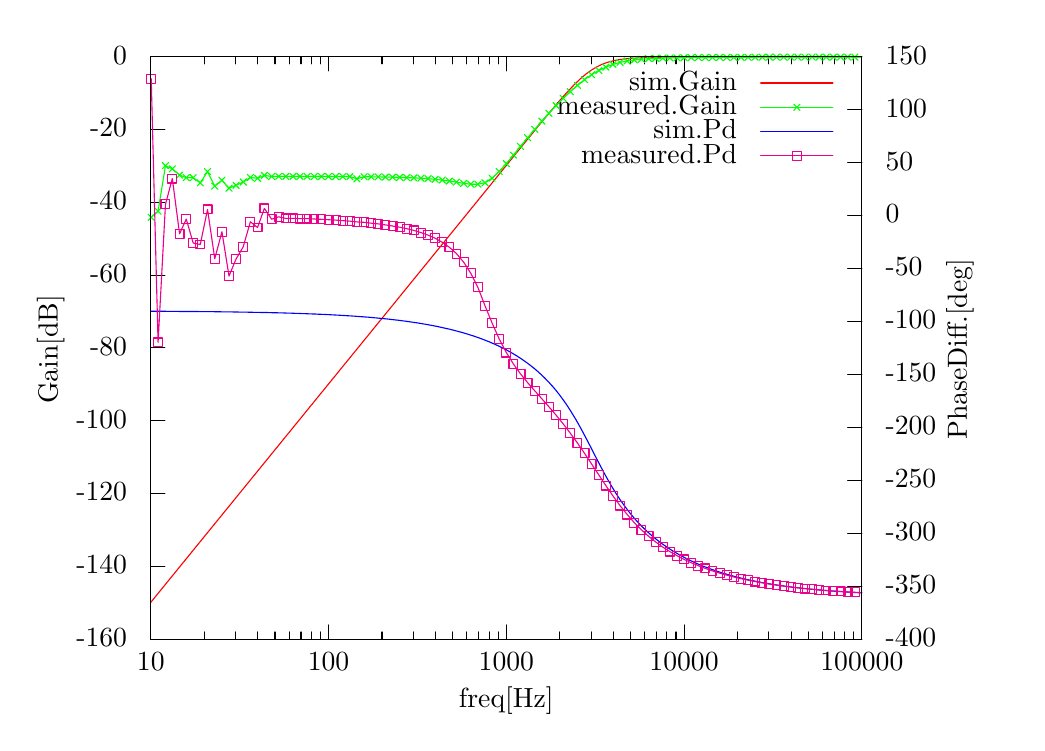
\begin{tikzpicture}[gnuplot]
%% generated with GNUPLOT 4.6p4 (Lua 5.1; terminal rev. 99, script rev. 100)
%% 2016年06月18日 10時15分32秒
\path (0.000,0.000) rectangle (12.500,8.750);
\gpcolor{color=gp lt color border}
\gpsetlinetype{gp lt border}
\gpsetlinewidth{1.00}
\draw[gp path] (1.504,0.985)--(1.684,0.985);
\node[gp node right] at (1.320,0.985) {-160};
\draw[gp path] (1.504,1.910)--(1.684,1.910);
\node[gp node right] at (1.320,1.910) {-140};
\draw[gp path] (1.504,2.834)--(1.684,2.834);
\node[gp node right] at (1.320,2.834) {-120};
\draw[gp path] (1.504,3.759)--(1.684,3.759);
\node[gp node right] at (1.320,3.759) {-100};
\draw[gp path] (1.504,4.683)--(1.684,4.683);
\node[gp node right] at (1.320,4.683) {-80};
\draw[gp path] (1.504,5.608)--(1.684,5.608);
\node[gp node right] at (1.320,5.608) {-60};
\draw[gp path] (1.504,6.532)--(1.684,6.532);
\node[gp node right] at (1.320,6.532) {-40};
\draw[gp path] (1.504,7.457)--(1.684,7.457);
\node[gp node right] at (1.320,7.457) {-20};
\draw[gp path] (1.504,8.381)--(1.684,8.381);
\node[gp node right] at (1.320,8.381) { 0};
\draw[gp path] (1.504,0.985)--(1.504,1.165);
\draw[gp path] (1.504,8.381)--(1.504,8.201);
\node[gp node center] at (1.504,0.677) { 10};
\draw[gp path] (2.184,0.985)--(2.184,1.075);
\draw[gp path] (2.184,8.381)--(2.184,8.291);
\draw[gp path] (2.581,0.985)--(2.581,1.075);
\draw[gp path] (2.581,8.381)--(2.581,8.291);
\draw[gp path] (2.863,0.985)--(2.863,1.075);
\draw[gp path] (2.863,8.381)--(2.863,8.291);
\draw[gp path] (3.082,0.985)--(3.082,1.075);
\draw[gp path] (3.082,8.381)--(3.082,8.291);
\draw[gp path] (3.261,0.985)--(3.261,1.075);
\draw[gp path] (3.261,8.381)--(3.261,8.291);
\draw[gp path] (3.412,0.985)--(3.412,1.075);
\draw[gp path] (3.412,8.381)--(3.412,8.291);
\draw[gp path] (3.543,0.985)--(3.543,1.075);
\draw[gp path] (3.543,8.381)--(3.543,8.291);
\draw[gp path] (3.658,0.985)--(3.658,1.075);
\draw[gp path] (3.658,8.381)--(3.658,8.291);
\draw[gp path] (3.762,0.985)--(3.762,1.165);
\draw[gp path] (3.762,8.381)--(3.762,8.201);
\node[gp node center] at (3.762,0.677) { 100};
\draw[gp path] (4.441,0.985)--(4.441,1.075);
\draw[gp path] (4.441,8.381)--(4.441,8.291);
\draw[gp path] (4.839,0.985)--(4.839,1.075);
\draw[gp path] (4.839,8.381)--(4.839,8.291);
\draw[gp path] (5.121,0.985)--(5.121,1.075);
\draw[gp path] (5.121,8.381)--(5.121,8.291);
\draw[gp path] (5.340,0.985)--(5.340,1.075);
\draw[gp path] (5.340,8.381)--(5.340,8.291);
\draw[gp path] (5.519,0.985)--(5.519,1.075);
\draw[gp path] (5.519,8.381)--(5.519,8.291);
\draw[gp path] (5.670,0.985)--(5.670,1.075);
\draw[gp path] (5.670,8.381)--(5.670,8.291);
\draw[gp path] (5.801,0.985)--(5.801,1.075);
\draw[gp path] (5.801,8.381)--(5.801,8.291);
\draw[gp path] (5.916,0.985)--(5.916,1.075);
\draw[gp path] (5.916,8.381)--(5.916,8.291);
\draw[gp path] (6.020,0.985)--(6.020,1.165);
\draw[gp path] (6.020,8.381)--(6.020,8.201);
\node[gp node center] at (6.020,0.677) { 1000};
\draw[gp path] (6.699,0.985)--(6.699,1.075);
\draw[gp path] (6.699,8.381)--(6.699,8.291);
\draw[gp path] (7.097,0.985)--(7.097,1.075);
\draw[gp path] (7.097,8.381)--(7.097,8.291);
\draw[gp path] (7.379,0.985)--(7.379,1.075);
\draw[gp path] (7.379,8.381)--(7.379,8.291);
\draw[gp path] (7.598,0.985)--(7.598,1.075);
\draw[gp path] (7.598,8.381)--(7.598,8.291);
\draw[gp path] (7.776,0.985)--(7.776,1.075);
\draw[gp path] (7.776,8.381)--(7.776,8.291);
\draw[gp path] (7.928,0.985)--(7.928,1.075);
\draw[gp path] (7.928,8.381)--(7.928,8.291);
\draw[gp path] (8.058,0.985)--(8.058,1.075);
\draw[gp path] (8.058,8.381)--(8.058,8.291);
\draw[gp path] (8.174,0.985)--(8.174,1.075);
\draw[gp path] (8.174,8.381)--(8.174,8.291);
\draw[gp path] (8.277,0.985)--(8.277,1.165);
\draw[gp path] (8.277,8.381)--(8.277,8.201);
\node[gp node center] at (8.277,0.677) { 10000};
\draw[gp path] (8.957,0.985)--(8.957,1.075);
\draw[gp path] (8.957,8.381)--(8.957,8.291);
\draw[gp path] (9.354,0.985)--(9.354,1.075);
\draw[gp path] (9.354,8.381)--(9.354,8.291);
\draw[gp path] (9.637,0.985)--(9.637,1.075);
\draw[gp path] (9.637,8.381)--(9.637,8.291);
\draw[gp path] (9.855,0.985)--(9.855,1.075);
\draw[gp path] (9.855,8.381)--(9.855,8.291);
\draw[gp path] (10.034,0.985)--(10.034,1.075);
\draw[gp path] (10.034,8.381)--(10.034,8.291);
\draw[gp path] (10.185,0.985)--(10.185,1.075);
\draw[gp path] (10.185,8.381)--(10.185,8.291);
\draw[gp path] (10.316,0.985)--(10.316,1.075);
\draw[gp path] (10.316,8.381)--(10.316,8.291);
\draw[gp path] (10.432,0.985)--(10.432,1.075);
\draw[gp path] (10.432,8.381)--(10.432,8.291);
\draw[gp path] (10.535,0.985)--(10.535,1.165);
\draw[gp path] (10.535,8.381)--(10.535,8.201);
\node[gp node center] at (10.535,0.677) { 100000};
\draw[gp path] (10.535,0.985)--(10.355,0.985);
\node[gp node left] at (10.719,0.985) {-400};
\draw[gp path] (10.535,1.657)--(10.355,1.657);
\node[gp node left] at (10.719,1.657) {-350};
\draw[gp path] (10.535,2.330)--(10.355,2.330);
\node[gp node left] at (10.719,2.330) {-300};
\draw[gp path] (10.535,3.002)--(10.355,3.002);
\node[gp node left] at (10.719,3.002) {-250};
\draw[gp path] (10.535,3.674)--(10.355,3.674);
\node[gp node left] at (10.719,3.674) {-200};
\draw[gp path] (10.535,4.347)--(10.355,4.347);
\node[gp node left] at (10.719,4.347) {-150};
\draw[gp path] (10.535,5.019)--(10.355,5.019);
\node[gp node left] at (10.719,5.019) {-100};
\draw[gp path] (10.535,5.692)--(10.355,5.692);
\node[gp node left] at (10.719,5.692) {-50};
\draw[gp path] (10.535,6.364)--(10.355,6.364);
\node[gp node left] at (10.719,6.364) { 0};
\draw[gp path] (10.535,7.036)--(10.355,7.036);
\node[gp node left] at (10.719,7.036) { 50};
\draw[gp path] (10.535,7.709)--(10.355,7.709);
\node[gp node left] at (10.719,7.709) { 100};
\draw[gp path] (10.535,8.381)--(10.355,8.381);
\node[gp node left] at (10.719,8.381) { 150};
\draw[gp path] (1.504,8.381)--(1.504,0.985)--(10.535,0.985)--(10.535,8.381)--cycle;
\node[gp node center,rotate=-270] at (0.246,4.683) {Gain[dB]};
\node[gp node center,rotate=-270] at (11.792,4.683) {PhaseDiff.[deg]};
\node[gp node center] at (6.019,0.215) {freq[Hz]};
\node[gp node right] at (9.067,8.047) {sim.Gain};
\gpcolor{color=gp lt color 0}
\gpsetlinetype{gp lt plot 0}
\draw[gp path] (9.251,8.047)--(10.167,8.047);
\draw[gp path] (1.504,1.451)--(1.509,1.457)--(1.513,1.462)--(1.518,1.468)--(1.522,1.473)%
  --(1.527,1.479)--(1.531,1.484)--(1.536,1.490)--(1.540,1.495)--(1.545,1.501)--(1.549,1.507)%
  --(1.554,1.512)--(1.558,1.518)--(1.563,1.523)--(1.567,1.529)--(1.572,1.534)--(1.576,1.540)%
  --(1.581,1.545)--(1.585,1.551)--(1.590,1.556)--(1.594,1.562)--(1.599,1.568)--(1.603,1.573)%
  --(1.608,1.579)--(1.612,1.584)--(1.617,1.590)--(1.621,1.595)--(1.626,1.601)--(1.630,1.606)%
  --(1.635,1.612)--(1.639,1.617)--(1.644,1.623)--(1.648,1.629)--(1.653,1.634)--(1.658,1.640)%
  --(1.662,1.645)--(1.667,1.651)--(1.671,1.656)--(1.676,1.662)--(1.680,1.667)--(1.685,1.673)%
  --(1.689,1.678)--(1.694,1.684)--(1.698,1.690)--(1.703,1.695)--(1.707,1.701)--(1.712,1.706)%
  --(1.716,1.712)--(1.721,1.717)--(1.725,1.723)--(1.730,1.728)--(1.734,1.734)--(1.739,1.740)%
  --(1.743,1.745)--(1.748,1.751)--(1.752,1.756)--(1.757,1.762)--(1.761,1.767)--(1.766,1.773)%
  --(1.770,1.778)--(1.775,1.784)--(1.779,1.789)--(1.784,1.795)--(1.788,1.801)--(1.793,1.806)%
  --(1.798,1.812)--(1.802,1.817)--(1.807,1.823)--(1.811,1.828)--(1.816,1.834)--(1.820,1.839)%
  --(1.825,1.845)--(1.829,1.850)--(1.834,1.856)--(1.838,1.862)--(1.843,1.867)--(1.847,1.873)%
  --(1.852,1.878)--(1.856,1.884)--(1.861,1.889)--(1.865,1.895)--(1.870,1.900)--(1.874,1.906)%
  --(1.879,1.911)--(1.883,1.917)--(1.888,1.923)--(1.892,1.928)--(1.897,1.934)--(1.901,1.939)%
  --(1.906,1.945)--(1.910,1.950)--(1.915,1.956)--(1.919,1.961)--(1.924,1.967)--(1.928,1.972)%
  --(1.933,1.978)--(1.937,1.984)--(1.942,1.989)--(1.947,1.995)--(1.951,2.000)--(1.956,2.006)%
  --(1.960,2.011)--(1.965,2.017)--(1.969,2.022)--(1.974,2.028)--(1.978,2.033)--(1.983,2.039)%
  --(1.987,2.045)--(1.992,2.050)--(1.996,2.056)--(2.001,2.061)--(2.005,2.067)--(2.010,2.072)%
  --(2.014,2.078)--(2.019,2.083)--(2.023,2.089)--(2.028,2.095)--(2.032,2.100)--(2.037,2.106)%
  --(2.041,2.111)--(2.046,2.117)--(2.050,2.122)--(2.055,2.128)--(2.059,2.133)--(2.064,2.139)%
  --(2.068,2.144)--(2.073,2.150)--(2.077,2.156)--(2.082,2.161)--(2.086,2.167)--(2.091,2.172)%
  --(2.096,2.178)--(2.100,2.183)--(2.105,2.189)--(2.109,2.194)--(2.114,2.200)--(2.118,2.205)%
  --(2.123,2.211)--(2.127,2.217)--(2.132,2.222)--(2.136,2.228)--(2.141,2.233)--(2.145,2.239)%
  --(2.150,2.244)--(2.154,2.250)--(2.159,2.255)--(2.163,2.261)--(2.168,2.266)--(2.172,2.272)%
  --(2.177,2.278)--(2.181,2.283)--(2.186,2.289)--(2.190,2.294)--(2.195,2.300)--(2.199,2.305)%
  --(2.204,2.311)--(2.208,2.316)--(2.213,2.322)--(2.217,2.327)--(2.222,2.333)--(2.226,2.339)%
  --(2.231,2.344)--(2.236,2.350)--(2.240,2.355)--(2.245,2.361)--(2.249,2.366)--(2.254,2.372)%
  --(2.258,2.377)--(2.263,2.383)--(2.267,2.389)--(2.272,2.394)--(2.276,2.400)--(2.281,2.405)%
  --(2.285,2.411)--(2.290,2.416)--(2.294,2.422)--(2.299,2.427)--(2.303,2.433)--(2.308,2.438)%
  --(2.312,2.444)--(2.317,2.450)--(2.321,2.455)--(2.326,2.461)--(2.330,2.466)--(2.335,2.472)%
  --(2.339,2.477)--(2.344,2.483)--(2.348,2.488)--(2.353,2.494)--(2.357,2.499)--(2.362,2.505)%
  --(2.366,2.511)--(2.371,2.516)--(2.375,2.522)--(2.380,2.527)--(2.385,2.533)--(2.389,2.538)%
  --(2.394,2.544)--(2.398,2.549)--(2.403,2.555)--(2.407,2.560)--(2.412,2.566)--(2.416,2.572)%
  --(2.421,2.577)--(2.425,2.583)--(2.430,2.588)--(2.434,2.594)--(2.439,2.599)--(2.443,2.605)%
  --(2.448,2.610)--(2.452,2.616)--(2.457,2.621)--(2.461,2.627)--(2.466,2.633)--(2.470,2.638)%
  --(2.475,2.644)--(2.479,2.649)--(2.484,2.655)--(2.488,2.660)--(2.493,2.666)--(2.497,2.671)%
  --(2.502,2.677)--(2.506,2.682)--(2.511,2.688)--(2.515,2.694)--(2.520,2.699)--(2.525,2.705)%
  --(2.529,2.710)--(2.534,2.716)--(2.538,2.721)--(2.543,2.727)--(2.547,2.732)--(2.552,2.738)%
  --(2.556,2.744)--(2.561,2.749)--(2.565,2.755)--(2.570,2.760)--(2.574,2.766)--(2.579,2.771)%
  --(2.583,2.777)--(2.588,2.782)--(2.592,2.788)--(2.597,2.793)--(2.601,2.799)--(2.606,2.805)%
  --(2.610,2.810)--(2.615,2.816)--(2.619,2.821)--(2.624,2.827)--(2.628,2.832)--(2.633,2.838)%
  --(2.637,2.843)--(2.642,2.849)--(2.646,2.854)--(2.651,2.860)--(2.655,2.866)--(2.660,2.871)%
  --(2.664,2.877)--(2.669,2.882)--(2.674,2.888)--(2.678,2.893)--(2.683,2.899)--(2.687,2.904)%
  --(2.692,2.910)--(2.696,2.915)--(2.701,2.921)--(2.705,2.927)--(2.710,2.932)--(2.714,2.938)%
  --(2.719,2.943)--(2.723,2.949)--(2.728,2.954)--(2.732,2.960)--(2.737,2.965)--(2.741,2.971)%
  --(2.746,2.976)--(2.750,2.982)--(2.755,2.988)--(2.759,2.993)--(2.764,2.999)--(2.768,3.004)%
  --(2.773,3.010)--(2.777,3.015)--(2.782,3.021)--(2.786,3.026)--(2.791,3.032)--(2.795,3.038)%
  --(2.800,3.043)--(2.804,3.049)--(2.809,3.054)--(2.813,3.060)--(2.818,3.065)--(2.823,3.071)%
  --(2.827,3.076)--(2.832,3.082)--(2.836,3.087)--(2.841,3.093)--(2.845,3.099)--(2.850,3.104)%
  --(2.854,3.110)--(2.859,3.115)--(2.863,3.121)--(2.868,3.126)--(2.872,3.132)--(2.877,3.137)%
  --(2.881,3.143)--(2.886,3.148)--(2.890,3.154)--(2.895,3.160)--(2.899,3.165)--(2.904,3.171)%
  --(2.908,3.176)--(2.913,3.182)--(2.917,3.187)--(2.922,3.193)--(2.926,3.198)--(2.931,3.204)%
  --(2.935,3.209)--(2.940,3.215)--(2.944,3.221)--(2.949,3.226)--(2.953,3.232)--(2.958,3.237)%
  --(2.963,3.243)--(2.967,3.248)--(2.972,3.254)--(2.976,3.259)--(2.981,3.265)--(2.985,3.270)%
  --(2.990,3.276)--(2.994,3.282)--(2.999,3.287)--(3.003,3.293)--(3.008,3.298)--(3.012,3.304)%
  --(3.017,3.309)--(3.021,3.315)--(3.026,3.320)--(3.030,3.326)--(3.035,3.331)--(3.039,3.337)%
  --(3.044,3.343)--(3.048,3.348)--(3.053,3.354)--(3.057,3.359)--(3.062,3.365)--(3.066,3.370)%
  --(3.071,3.376)--(3.075,3.381)--(3.080,3.387)--(3.084,3.393)--(3.089,3.398)--(3.093,3.404)%
  --(3.098,3.409)--(3.102,3.415)--(3.107,3.420)--(3.112,3.426)--(3.116,3.431)--(3.121,3.437)%
  --(3.125,3.442)--(3.130,3.448)--(3.134,3.454)--(3.139,3.459)--(3.143,3.465)--(3.148,3.470)%
  --(3.152,3.476)--(3.157,3.481)--(3.161,3.487)--(3.166,3.492)--(3.170,3.498)--(3.175,3.503)%
  --(3.179,3.509)--(3.184,3.515)--(3.188,3.520)--(3.193,3.526)--(3.197,3.531)--(3.202,3.537)%
  --(3.206,3.542)--(3.211,3.548)--(3.215,3.553)--(3.220,3.559)--(3.224,3.564)--(3.229,3.570)%
  --(3.233,3.576)--(3.238,3.581)--(3.242,3.587)--(3.247,3.592)--(3.251,3.598)--(3.256,3.603)%
  --(3.261,3.609)--(3.265,3.614)--(3.270,3.620)--(3.274,3.625)--(3.279,3.631)--(3.283,3.637)%
  --(3.288,3.642)--(3.292,3.648)--(3.297,3.653)--(3.301,3.659)--(3.306,3.664)--(3.310,3.670)%
  --(3.315,3.675)--(3.319,3.681)--(3.324,3.687)--(3.328,3.692)--(3.333,3.698)--(3.337,3.703)%
  --(3.342,3.709)--(3.346,3.714)--(3.351,3.720)--(3.355,3.725)--(3.360,3.731)--(3.364,3.736)%
  --(3.369,3.742)--(3.373,3.748)--(3.378,3.753)--(3.382,3.759)--(3.387,3.764)--(3.391,3.770)%
  --(3.396,3.775)--(3.401,3.781)--(3.405,3.786)--(3.410,3.792)--(3.414,3.797)--(3.419,3.803)%
  --(3.423,3.809)--(3.428,3.814)--(3.432,3.820)--(3.437,3.825)--(3.441,3.831)--(3.446,3.836)%
  --(3.450,3.842)--(3.455,3.847)--(3.459,3.853)--(3.464,3.858)--(3.468,3.864)--(3.473,3.870)%
  --(3.477,3.875)--(3.482,3.881)--(3.486,3.886)--(3.491,3.892)--(3.495,3.897)--(3.500,3.903)%
  --(3.504,3.908)--(3.509,3.914)--(3.513,3.919)--(3.518,3.925)--(3.522,3.931)--(3.527,3.936)%
  --(3.531,3.942)--(3.536,3.947)--(3.540,3.953)--(3.545,3.958)--(3.550,3.964)--(3.554,3.969)%
  --(3.559,3.975)--(3.563,3.981)--(3.568,3.986)--(3.572,3.992)--(3.577,3.997)--(3.581,4.003)%
  --(3.586,4.008)--(3.590,4.014)--(3.595,4.019)--(3.599,4.025)--(3.604,4.030)--(3.608,4.036)%
  --(3.613,4.042)--(3.617,4.047)--(3.622,4.053)--(3.626,4.058)--(3.631,4.064)--(3.635,4.069)%
  --(3.640,4.075)--(3.644,4.080)--(3.649,4.086)--(3.653,4.091)--(3.658,4.097)--(3.662,4.103)%
  --(3.667,4.108)--(3.671,4.114)--(3.676,4.119)--(3.680,4.125)--(3.685,4.130)--(3.690,4.136)%
  --(3.694,4.141)--(3.699,4.147)--(3.703,4.152)--(3.708,4.158)--(3.712,4.164)--(3.717,4.169)%
  --(3.721,4.175)--(3.726,4.180)--(3.730,4.186)--(3.735,4.191)--(3.739,4.197)--(3.744,4.202)%
  --(3.748,4.208)--(3.753,4.213)--(3.757,4.219)--(3.762,4.225)--(3.766,4.230)--(3.771,4.236)%
  --(3.775,4.241)--(3.780,4.247)--(3.784,4.252)--(3.789,4.258)--(3.793,4.263)--(3.798,4.269)%
  --(3.802,4.275)--(3.807,4.280)--(3.811,4.286)--(3.816,4.291)--(3.820,4.297)--(3.825,4.302)%
  --(3.829,4.308)--(3.834,4.313)--(3.839,4.319)--(3.843,4.324)--(3.848,4.330)--(3.852,4.336)%
  --(3.857,4.341)--(3.861,4.347)--(3.866,4.352)--(3.870,4.358)--(3.875,4.363)--(3.879,4.369)%
  --(3.884,4.374)--(3.888,4.380)--(3.893,4.385)--(3.897,4.391)--(3.902,4.397)--(3.906,4.402)%
  --(3.911,4.408)--(3.915,4.413)--(3.920,4.419)--(3.924,4.424)--(3.929,4.430)--(3.933,4.435)%
  --(3.938,4.441)--(3.942,4.446)--(3.947,4.452)--(3.951,4.458)--(3.956,4.463)--(3.960,4.469)%
  --(3.965,4.474)--(3.969,4.480)--(3.974,4.485)--(3.978,4.491)--(3.983,4.496)--(3.988,4.502)%
  --(3.992,4.508)--(3.997,4.513)--(4.001,4.519)--(4.006,4.524)--(4.010,4.530)--(4.015,4.535)%
  --(4.019,4.541)--(4.024,4.546)--(4.028,4.552)--(4.033,4.557)--(4.037,4.563)--(4.042,4.569)%
  --(4.046,4.574)--(4.051,4.580)--(4.055,4.585)--(4.060,4.591)--(4.064,4.596)--(4.069,4.602)%
  --(4.073,4.607)--(4.078,4.613)--(4.082,4.618)--(4.087,4.624)--(4.091,4.630)--(4.096,4.635)%
  --(4.100,4.641)--(4.105,4.646)--(4.109,4.652)--(4.114,4.657)--(4.118,4.663)--(4.123,4.668)%
  --(4.128,4.674)--(4.132,4.679)--(4.137,4.685)--(4.141,4.691)--(4.146,4.696)--(4.150,4.702)%
  --(4.155,4.707)--(4.159,4.713)--(4.164,4.718)--(4.168,4.724)--(4.173,4.729)--(4.177,4.735)%
  --(4.182,4.740)--(4.186,4.746)--(4.191,4.752)--(4.195,4.757)--(4.200,4.763)--(4.204,4.768)%
  --(4.209,4.774)--(4.213,4.779)--(4.218,4.785)--(4.222,4.790)--(4.227,4.796)--(4.231,4.802)%
  --(4.236,4.807)--(4.240,4.813)--(4.245,4.818)--(4.249,4.824)--(4.254,4.829)--(4.258,4.835)%
  --(4.263,4.840)--(4.267,4.846)--(4.272,4.851)--(4.277,4.857)--(4.281,4.863)--(4.286,4.868)%
  --(4.290,4.874)--(4.295,4.879)--(4.299,4.885)--(4.304,4.890)--(4.308,4.896)--(4.313,4.901)%
  --(4.317,4.907)--(4.322,4.912)--(4.326,4.918)--(4.331,4.924)--(4.335,4.929)--(4.340,4.935)%
  --(4.344,4.940)--(4.349,4.946)--(4.353,4.951)--(4.358,4.957)--(4.362,4.962)--(4.367,4.968)%
  --(4.371,4.974)--(4.376,4.979)--(4.380,4.985)--(4.385,4.990)--(4.389,4.996)--(4.394,5.001)%
  --(4.398,5.007)--(4.403,5.012)--(4.407,5.018)--(4.412,5.023)--(4.416,5.029)--(4.421,5.035)%
  --(4.426,5.040)--(4.430,5.046)--(4.435,5.051)--(4.439,5.057)--(4.444,5.062)--(4.448,5.068)%
  --(4.453,5.073)--(4.457,5.079)--(4.462,5.084)--(4.466,5.090)--(4.471,5.096)--(4.475,5.101)%
  --(4.480,5.107)--(4.484,5.112)--(4.489,5.118)--(4.493,5.123)--(4.498,5.129)--(4.502,5.134)%
  --(4.507,5.140)--(4.511,5.145)--(4.516,5.151)--(4.520,5.157)--(4.525,5.162)--(4.529,5.168)%
  --(4.534,5.173)--(4.538,5.179)--(4.543,5.184)--(4.547,5.190)--(4.552,5.195)--(4.556,5.201)%
  --(4.561,5.207)--(4.566,5.212)--(4.570,5.218)--(4.575,5.223)--(4.579,5.229)--(4.584,5.234)%
  --(4.588,5.240)--(4.593,5.245)--(4.597,5.251)--(4.602,5.256)--(4.606,5.262)--(4.611,5.268)%
  --(4.615,5.273)--(4.620,5.279)--(4.624,5.284)--(4.629,5.290)--(4.633,5.295)--(4.638,5.301)%
  --(4.642,5.306)--(4.647,5.312)--(4.651,5.317)--(4.656,5.323)--(4.660,5.329)--(4.665,5.334)%
  --(4.669,5.340)--(4.674,5.345)--(4.678,5.351)--(4.683,5.356)--(4.687,5.362)--(4.692,5.367)%
  --(4.696,5.373)--(4.701,5.379)--(4.705,5.384)--(4.710,5.390)--(4.715,5.395)--(4.719,5.401)%
  --(4.724,5.406)--(4.728,5.412)--(4.733,5.417)--(4.737,5.423)--(4.742,5.428)--(4.746,5.434)%
  --(4.751,5.440)--(4.755,5.445)--(4.760,5.451)--(4.764,5.456)--(4.769,5.462)--(4.773,5.467)%
  --(4.778,5.473)--(4.782,5.478)--(4.787,5.484)--(4.791,5.490)--(4.796,5.495)--(4.800,5.501)%
  --(4.805,5.506)--(4.809,5.512)--(4.814,5.517)--(4.818,5.523)--(4.823,5.528)--(4.827,5.534)%
  --(4.832,5.539)--(4.836,5.545)--(4.841,5.551)--(4.845,5.556)--(4.850,5.562)--(4.855,5.567)%
  --(4.859,5.573)--(4.864,5.578)--(4.868,5.584)--(4.873,5.589)--(4.877,5.595)--(4.882,5.601)%
  --(4.886,5.606)--(4.891,5.612)--(4.895,5.617)--(4.900,5.623)--(4.904,5.628)--(4.909,5.634)%
  --(4.913,5.639)--(4.918,5.645)--(4.922,5.650)--(4.927,5.656)--(4.931,5.662)--(4.936,5.667)%
  --(4.940,5.673)--(4.945,5.678)--(4.949,5.684)--(4.954,5.689)--(4.958,5.695)--(4.963,5.700)%
  --(4.967,5.706)--(4.972,5.711)--(4.976,5.717)--(4.981,5.723)--(4.985,5.728)--(4.990,5.734)%
  --(4.994,5.739)--(4.999,5.745)--(5.004,5.750)--(5.008,5.756)--(5.013,5.761)--(5.017,5.767)%
  --(5.022,5.773)--(5.026,5.778)--(5.031,5.784)--(5.035,5.789)--(5.040,5.795)--(5.044,5.800)%
  --(5.049,5.806)--(5.053,5.811)--(5.058,5.817)--(5.062,5.823)--(5.067,5.828)--(5.071,5.834)%
  --(5.076,5.839)--(5.080,5.845)--(5.085,5.850)--(5.089,5.856)--(5.094,5.861)--(5.098,5.867)%
  --(5.103,5.872)--(5.107,5.878)--(5.112,5.884)--(5.116,5.889)--(5.121,5.895)--(5.125,5.900)%
  --(5.130,5.906)--(5.134,5.911)--(5.139,5.917)--(5.143,5.922)--(5.148,5.928)--(5.153,5.934)%
  --(5.157,5.939)--(5.162,5.945)--(5.166,5.950)--(5.171,5.956)--(5.175,5.961)--(5.180,5.967)%
  --(5.184,5.972)--(5.189,5.978)--(5.193,5.983)--(5.198,5.989)--(5.202,5.995)--(5.207,6.000)%
  --(5.211,6.006)--(5.216,6.011)--(5.220,6.017)--(5.225,6.022)--(5.229,6.028)--(5.234,6.033)%
  --(5.238,6.039)--(5.243,6.045)--(5.247,6.050)--(5.252,6.056)--(5.256,6.061)--(5.261,6.067)%
  --(5.265,6.072)--(5.270,6.078)--(5.274,6.083)--(5.279,6.089)--(5.283,6.095)--(5.288,6.100)%
  --(5.293,6.106)--(5.297,6.111)--(5.302,6.117)--(5.306,6.122)--(5.311,6.128)--(5.315,6.133)%
  --(5.320,6.139)--(5.324,6.145)--(5.329,6.150)--(5.333,6.156)--(5.338,6.161)--(5.342,6.167)%
  --(5.347,6.172)--(5.351,6.178)--(5.356,6.183)--(5.360,6.189)--(5.365,6.194)--(5.369,6.200)%
  --(5.374,6.206)--(5.378,6.211)--(5.383,6.217)--(5.387,6.222)--(5.392,6.228)--(5.396,6.233)%
  --(5.401,6.239)--(5.405,6.244)--(5.410,6.250)--(5.414,6.256)--(5.419,6.261)--(5.423,6.267)%
  --(5.428,6.272)--(5.432,6.278)--(5.437,6.283)--(5.442,6.289)--(5.446,6.294)--(5.451,6.300)%
  --(5.455,6.306)--(5.460,6.311)--(5.464,6.317)--(5.469,6.322)--(5.473,6.328)--(5.478,6.333)%
  --(5.482,6.339)--(5.487,6.344)--(5.491,6.350)--(5.496,6.356)--(5.500,6.361)--(5.505,6.367)%
  --(5.509,6.372)--(5.514,6.378)--(5.518,6.383)--(5.523,6.389)--(5.527,6.394)--(5.532,6.400)%
  --(5.536,6.406)--(5.541,6.411)--(5.545,6.417)--(5.550,6.422)--(5.554,6.428)--(5.559,6.433)%
  --(5.563,6.439)--(5.568,6.444)--(5.572,6.450)--(5.577,6.456)--(5.581,6.461)--(5.586,6.467)%
  --(5.591,6.472)--(5.595,6.478)--(5.600,6.483)--(5.604,6.489)--(5.609,6.494)--(5.613,6.500)%
  --(5.618,6.506)--(5.622,6.511)--(5.627,6.517)--(5.631,6.522)--(5.636,6.528)--(5.640,6.533)%
  --(5.645,6.539)--(5.649,6.544)--(5.654,6.550)--(5.658,6.556)--(5.663,6.561)--(5.667,6.567)%
  --(5.672,6.572)--(5.676,6.578)--(5.681,6.583)--(5.685,6.589)--(5.690,6.595)--(5.694,6.600)%
  --(5.699,6.606)--(5.703,6.611)--(5.708,6.617)--(5.712,6.622)--(5.717,6.628)--(5.721,6.633)%
  --(5.726,6.639)--(5.731,6.645)--(5.735,6.650)--(5.740,6.656)--(5.744,6.661)--(5.749,6.667)%
  --(5.753,6.672)--(5.758,6.678)--(5.762,6.683)--(5.767,6.689)--(5.771,6.695)--(5.776,6.700)%
  --(5.780,6.706)--(5.785,6.711)--(5.789,6.717)--(5.794,6.722)--(5.798,6.728)--(5.803,6.734)%
  --(5.807,6.739)--(5.812,6.745)--(5.816,6.750)--(5.821,6.756)--(5.825,6.761)--(5.830,6.767)%
  --(5.834,6.772)--(5.839,6.778)--(5.843,6.784)--(5.848,6.789)--(5.852,6.795)--(5.857,6.800)%
  --(5.861,6.806)--(5.866,6.811)--(5.870,6.817)--(5.875,6.822)--(5.880,6.828)--(5.884,6.834)%
  --(5.889,6.839)--(5.893,6.845)--(5.898,6.850)--(5.902,6.856)--(5.907,6.861)--(5.911,6.867)%
  --(5.916,6.873)--(5.920,6.878)--(5.925,6.884)--(5.929,6.889)--(5.934,6.895)--(5.938,6.900)%
  --(5.943,6.906)--(5.947,6.911)--(5.952,6.917)--(5.956,6.923)--(5.961,6.928)--(5.965,6.934)%
  --(5.970,6.939)--(5.974,6.945)--(5.979,6.950)--(5.983,6.956)--(5.988,6.962)--(5.992,6.967)%
  --(5.997,6.973)--(6.001,6.978)--(6.006,6.984)--(6.010,6.989)--(6.015,6.995)--(6.020,7.000)%
  --(6.024,7.006)--(6.029,7.012)--(6.033,7.017)--(6.038,7.023)--(6.042,7.028)--(6.047,7.034)%
  --(6.051,7.039)--(6.056,7.045)--(6.060,7.051)--(6.065,7.056)--(6.069,7.062)--(6.074,7.067)%
  --(6.078,7.073)--(6.083,7.078)--(6.087,7.084)--(6.092,7.089)--(6.096,7.095)--(6.101,7.101)%
  --(6.105,7.106)--(6.110,7.112)--(6.114,7.117)--(6.119,7.123)--(6.123,7.128)--(6.128,7.134)%
  --(6.132,7.139)--(6.137,7.145)--(6.141,7.151)--(6.146,7.156)--(6.150,7.162)--(6.155,7.167)%
  --(6.159,7.173)--(6.164,7.178)--(6.169,7.184)--(6.173,7.190)--(6.178,7.195)--(6.182,7.201)%
  --(6.187,7.206)--(6.191,7.212)--(6.196,7.217)--(6.200,7.223)--(6.205,7.228)--(6.209,7.234)%
  --(6.214,7.240)--(6.218,7.245)--(6.223,7.251)--(6.227,7.256)--(6.232,7.262)--(6.236,7.267)%
  --(6.241,7.273)--(6.245,7.278)--(6.250,7.284)--(6.254,7.289)--(6.259,7.295)--(6.263,7.301)%
  --(6.268,7.306)--(6.272,7.312)--(6.277,7.317)--(6.281,7.323)--(6.286,7.328)--(6.290,7.334)%
  --(6.295,7.339)--(6.299,7.345)--(6.304,7.351)--(6.308,7.356)--(6.313,7.362)--(6.318,7.367)%
  --(6.322,7.373)--(6.327,7.378)--(6.331,7.384)--(6.336,7.389)--(6.340,7.395)--(6.345,7.400)%
  --(6.349,7.406)--(6.354,7.411)--(6.358,7.417)--(6.363,7.422)--(6.367,7.428)--(6.372,7.434)%
  --(6.376,7.439)--(6.381,7.445)--(6.385,7.450)--(6.390,7.456)--(6.394,7.461)--(6.399,7.467)%
  --(6.403,7.472)--(6.408,7.478)--(6.412,7.483)--(6.417,7.489)--(6.421,7.494)--(6.426,7.500)%
  --(6.430,7.505)--(6.435,7.511)--(6.439,7.516)--(6.444,7.522)--(6.448,7.527)--(6.453,7.533)%
  --(6.458,7.538)--(6.462,7.544)--(6.467,7.549)--(6.471,7.555)--(6.476,7.560)--(6.480,7.566)%
  --(6.485,7.571)--(6.489,7.577)--(6.494,7.582)--(6.498,7.588)--(6.503,7.593)--(6.507,7.598)%
  --(6.512,7.604)--(6.516,7.609)--(6.521,7.615)--(6.525,7.620)--(6.530,7.626)--(6.534,7.631)%
  --(6.539,7.637)--(6.543,7.642)--(6.548,7.647)--(6.552,7.653)--(6.557,7.658)--(6.561,7.664)%
  --(6.566,7.669)--(6.570,7.675)--(6.575,7.680)--(6.579,7.685)--(6.584,7.691)--(6.588,7.696)%
  --(6.593,7.701)--(6.597,7.707)--(6.602,7.712)--(6.607,7.718)--(6.611,7.723)--(6.616,7.728)%
  --(6.620,7.734)--(6.625,7.739)--(6.629,7.744)--(6.634,7.750)--(6.638,7.755)--(6.643,7.760)%
  --(6.647,7.766)--(6.652,7.771)--(6.656,7.776)--(6.661,7.781)--(6.665,7.787)--(6.670,7.792)%
  --(6.674,7.797)--(6.679,7.802)--(6.683,7.808)--(6.688,7.813)--(6.692,7.818)--(6.697,7.823)%
  --(6.701,7.829)--(6.706,7.834)--(6.710,7.839)--(6.715,7.844)--(6.719,7.849)--(6.724,7.854)%
  --(6.728,7.860)--(6.733,7.865)--(6.737,7.870)--(6.742,7.875)--(6.746,7.880)--(6.751,7.885)%
  --(6.756,7.890)--(6.760,7.895)--(6.765,7.900)--(6.769,7.905)--(6.774,7.910)--(6.778,7.915)%
  --(6.783,7.920)--(6.787,7.925)--(6.792,7.930)--(6.796,7.935)--(6.801,7.940)--(6.805,7.945)%
  --(6.810,7.950)--(6.814,7.955)--(6.819,7.959)--(6.823,7.964)--(6.828,7.969)--(6.832,7.974)%
  --(6.837,7.979)--(6.841,7.983)--(6.846,7.988)--(6.850,7.993)--(6.855,7.997)--(6.859,8.002)%
  --(6.864,8.007)--(6.868,8.011)--(6.873,8.016)--(6.877,8.021)--(6.882,8.025)--(6.886,8.030)%
  --(6.891,8.034)--(6.896,8.039)--(6.900,8.043)--(6.905,8.048)--(6.909,8.052)--(6.914,8.056)%
  --(6.918,8.061)--(6.923,8.065)--(6.927,8.069)--(6.932,8.074)--(6.936,8.078)--(6.941,8.082)%
  --(6.945,8.086)--(6.950,8.090)--(6.954,8.095)--(6.959,8.099)--(6.963,8.103)--(6.968,8.107)%
  --(6.972,8.111)--(6.977,8.115)--(6.981,8.119)--(6.986,8.123)--(6.990,8.127)--(6.995,8.130)%
  --(6.999,8.134)--(7.004,8.138)--(7.008,8.142)--(7.013,8.146)--(7.017,8.149)--(7.022,8.153)%
  --(7.026,8.157)--(7.031,8.160)--(7.035,8.164)--(7.040,8.167)--(7.045,8.171)--(7.049,8.174)%
  --(7.054,8.177)--(7.058,8.181)--(7.063,8.184)--(7.067,8.187)--(7.072,8.191)--(7.076,8.194)%
  --(7.081,8.197)--(7.085,8.200)--(7.090,8.203)--(7.094,8.206)--(7.099,8.210)--(7.103,8.213)%
  --(7.108,8.215)--(7.112,8.218)--(7.117,8.221)--(7.121,8.224)--(7.126,8.227)--(7.130,8.230)%
  --(7.135,8.232)--(7.139,8.235)--(7.144,8.238)--(7.148,8.240)--(7.153,8.243)--(7.157,8.246)%
  --(7.162,8.248)--(7.166,8.250)--(7.171,8.253)--(7.175,8.255)--(7.180,8.258)--(7.184,8.260)%
  --(7.189,8.262)--(7.194,8.265)--(7.198,8.267)--(7.203,8.269)--(7.207,8.271)--(7.212,8.273)%
  --(7.216,8.275)--(7.221,8.277)--(7.225,8.279)--(7.230,8.281)--(7.234,8.283)--(7.239,8.285)%
  --(7.243,8.287)--(7.248,8.289)--(7.252,8.291)--(7.257,8.292)--(7.261,8.294)--(7.266,8.296)%
  --(7.270,8.297)--(7.275,8.299)--(7.279,8.301)--(7.284,8.302)--(7.288,8.304)--(7.293,8.305)%
  --(7.297,8.307)--(7.302,8.308)--(7.306,8.310)--(7.311,8.311)--(7.315,8.313)--(7.320,8.314)%
  --(7.324,8.315)--(7.329,8.317)--(7.334,8.318)--(7.338,8.319)--(7.343,8.320)--(7.347,8.321)%
  --(7.352,8.323)--(7.356,8.324)--(7.361,8.325)--(7.365,8.326)--(7.370,8.327)--(7.374,8.328)%
  --(7.379,8.329)--(7.383,8.330)--(7.388,8.331)--(7.392,8.332)--(7.397,8.333)--(7.401,8.334)%
  --(7.406,8.335)--(7.410,8.336)--(7.415,8.337)--(7.419,8.338)--(7.424,8.338)--(7.428,8.339)%
  --(7.433,8.340)--(7.437,8.341)--(7.442,8.342)--(7.446,8.342)--(7.451,8.343)--(7.455,8.344)%
  --(7.460,8.344)--(7.464,8.345)--(7.469,8.346)--(7.473,8.346)--(7.478,8.347)--(7.483,8.348)%
  --(7.487,8.348)--(7.492,8.349)--(7.496,8.350)--(7.501,8.350)--(7.505,8.351)--(7.510,8.351)%
  --(7.514,8.352)--(7.519,8.352)--(7.523,8.353)--(7.528,8.353)--(7.532,8.354)--(7.537,8.354)%
  --(7.541,8.355)--(7.546,8.355)--(7.550,8.356)--(7.555,8.356)--(7.559,8.357)--(7.564,8.357)%
  --(7.568,8.357)--(7.573,8.358)--(7.577,8.358)--(7.582,8.359)--(7.586,8.359)--(7.591,8.359)%
  --(7.595,8.360)--(7.600,8.360)--(7.604,8.360)--(7.609,8.361)--(7.613,8.361)--(7.618,8.361)%
  --(7.623,8.362)--(7.627,8.362)--(7.632,8.362)--(7.636,8.363)--(7.641,8.363)--(7.645,8.363)%
  --(7.650,8.364)--(7.654,8.364)--(7.659,8.364)--(7.663,8.364)--(7.668,8.365)--(7.672,8.365)%
  --(7.677,8.365)--(7.681,8.365)--(7.686,8.366)--(7.690,8.366)--(7.695,8.366)--(7.699,8.366)%
  --(7.704,8.366)--(7.708,8.367)--(7.713,8.367)--(7.717,8.367)--(7.722,8.367)--(7.726,8.367)%
  --(7.731,8.368)--(7.735,8.368)--(7.740,8.368)--(7.744,8.368)--(7.749,8.368)--(7.753,8.369)%
  --(7.758,8.369)--(7.762,8.369)--(7.767,8.369)--(7.772,8.369)--(7.776,8.369)--(7.781,8.370)%
  --(7.785,8.370)--(7.790,8.370)--(7.794,8.370)--(7.799,8.370)--(7.803,8.370)--(7.808,8.370)%
  --(7.812,8.371)--(7.817,8.371)--(7.821,8.371)--(7.826,8.371)--(7.830,8.371)--(7.835,8.371)%
  --(7.839,8.371)--(7.844,8.371)--(7.848,8.372)--(7.853,8.372)--(7.857,8.372)--(7.862,8.372)%
  --(7.866,8.372)--(7.871,8.372)--(7.875,8.372)--(7.880,8.372)--(7.884,8.372)--(7.889,8.373)%
  --(7.893,8.373)--(7.898,8.373)--(7.902,8.373)--(7.907,8.373)--(7.911,8.373)--(7.916,8.373)%
  --(7.921,8.373)--(7.925,8.373)--(7.930,8.373)--(7.934,8.374)--(7.939,8.374)--(7.943,8.374)%
  --(7.948,8.374)--(7.952,8.374)--(7.957,8.374)--(7.961,8.374)--(7.966,8.374)--(7.970,8.374)%
  --(7.975,8.374)--(7.979,8.374)--(7.984,8.374)--(7.988,8.374)--(7.993,8.375)--(7.997,8.375)%
  --(8.002,8.375)--(8.006,8.375)--(8.011,8.375)--(8.015,8.375)--(8.020,8.375)--(8.024,8.375)%
  --(8.029,8.375)--(8.033,8.375)--(8.038,8.375)--(8.042,8.375)--(8.047,8.375)--(8.051,8.375)%
  --(8.056,8.375)--(8.061,8.375)--(8.065,8.376)--(8.070,8.376)--(8.074,8.376)--(8.079,8.376)%
  --(8.083,8.376)--(8.088,8.376)--(8.092,8.376)--(8.097,8.376)--(8.101,8.376)--(8.106,8.376)%
  --(8.110,8.376)--(8.115,8.376)--(8.119,8.376)--(8.124,8.376)--(8.128,8.376)--(8.133,8.376)%
  --(8.137,8.376)--(8.142,8.376)--(8.146,8.376)--(8.151,8.376)--(8.155,8.377)--(8.160,8.377)%
  --(8.164,8.377)--(8.169,8.377)--(8.173,8.377)--(8.178,8.377)--(8.182,8.377)--(8.187,8.377)%
  --(8.191,8.377)--(8.196,8.377)--(8.200,8.377)--(8.205,8.377)--(8.210,8.377)--(8.214,8.377)%
  --(8.219,8.377)--(8.223,8.377)--(8.228,8.377)--(8.232,8.377)--(8.237,8.377)--(8.241,8.377)%
  --(8.246,8.377)--(8.250,8.377)--(8.255,8.377)--(8.259,8.377)--(8.264,8.377)--(8.268,8.377)%
  --(8.273,8.378)--(8.277,8.378)--(8.282,8.378)--(8.286,8.378)--(8.291,8.378)--(8.295,8.378)%
  --(8.300,8.378)--(8.304,8.378)--(8.309,8.378)--(8.313,8.378)--(8.318,8.378)--(8.322,8.378)%
  --(8.327,8.378)--(8.331,8.378)--(8.336,8.378)--(8.340,8.378)--(8.345,8.378)--(8.349,8.378)%
  --(8.354,8.378)--(8.359,8.378)--(8.363,8.378)--(8.368,8.378)--(8.372,8.378)--(8.377,8.378)%
  --(8.381,8.378)--(8.386,8.378)--(8.390,8.378)--(8.395,8.378)--(8.399,8.378)--(8.404,8.378)%
  --(8.408,8.378)--(8.413,8.378)--(8.417,8.378)--(8.422,8.378)--(8.426,8.378)--(8.431,8.378)%
  --(8.435,8.379)--(8.440,8.379)--(8.444,8.379)--(8.449,8.379)--(8.453,8.379)--(8.458,8.379)%
  --(8.462,8.379)--(8.467,8.379)--(8.471,8.379)--(8.476,8.379)--(8.480,8.379)--(8.485,8.379)%
  --(8.489,8.379)--(8.494,8.379)--(8.499,8.379)--(8.503,8.379)--(8.508,8.379)--(8.512,8.379)%
  --(8.517,8.379)--(8.521,8.379)--(8.526,8.379)--(8.530,8.379)--(8.535,8.379)--(8.539,8.379)%
  --(8.544,8.379)--(8.548,8.379)--(8.553,8.379)--(8.557,8.379)--(8.562,8.379)--(8.566,8.379)%
  --(8.571,8.379)--(8.575,8.379)--(8.580,8.379)--(8.584,8.379)--(8.589,8.379)--(8.593,8.379)%
  --(8.598,8.379)--(8.602,8.379)--(8.607,8.379)--(8.611,8.379)--(8.616,8.379)--(8.620,8.379)%
  --(8.625,8.379)--(8.629,8.379)--(8.634,8.379)--(8.638,8.379)--(8.643,8.379)--(8.648,8.379)%
  --(8.652,8.379)--(8.657,8.379)--(8.661,8.379)--(8.666,8.379)--(8.670,8.379)--(8.675,8.379)%
  --(8.679,8.379)--(8.684,8.379)--(8.688,8.379)--(8.693,8.380)--(8.697,8.380)--(8.702,8.380)%
  --(8.706,8.380)--(8.711,8.380)--(8.715,8.380)--(8.720,8.380)--(8.724,8.380)--(8.729,8.380)%
  --(8.733,8.380)--(8.738,8.380)--(8.742,8.380)--(8.747,8.380)--(8.751,8.380)--(8.756,8.380)%
  --(8.760,8.380)--(8.765,8.380)--(8.769,8.380)--(8.774,8.380)--(8.778,8.380)--(8.783,8.380)%
  --(8.788,8.380)--(8.792,8.380)--(8.797,8.380)--(8.801,8.380)--(8.806,8.380)--(8.810,8.380)%
  --(8.815,8.380)--(8.819,8.380)--(8.824,8.380)--(8.828,8.380)--(8.833,8.380)--(8.837,8.380)%
  --(8.842,8.380)--(8.846,8.380)--(8.851,8.380)--(8.855,8.380)--(8.860,8.380)--(8.864,8.380)%
  --(8.869,8.380)--(8.873,8.380)--(8.878,8.380)--(8.882,8.380)--(8.887,8.380)--(8.891,8.380)%
  --(8.896,8.380)--(8.900,8.380)--(8.905,8.380)--(8.909,8.380)--(8.914,8.380)--(8.918,8.380)%
  --(8.923,8.380)--(8.927,8.380)--(8.932,8.380)--(8.937,8.380)--(8.941,8.380)--(8.946,8.380)%
  --(8.950,8.380)--(8.955,8.380)--(8.959,8.380)--(8.964,8.380)--(8.968,8.380)--(8.973,8.380)%
  --(8.977,8.380)--(8.982,8.380)--(8.986,8.380)--(8.991,8.380)--(8.995,8.380)--(9.000,8.380)%
  --(9.004,8.380)--(9.009,8.380)--(9.013,8.380)--(9.018,8.380)--(9.022,8.380)--(9.027,8.380)%
  --(9.031,8.380)--(9.036,8.380)--(9.040,8.380)--(9.045,8.380)--(9.049,8.380)--(9.054,8.380)%
  --(9.058,8.380)--(9.063,8.380)--(9.067,8.380)--(9.072,8.380)--(9.076,8.380)--(9.081,8.380)%
  --(9.086,8.380)--(9.090,8.380)--(9.095,8.380)--(9.099,8.380)--(9.104,8.380)--(9.108,8.380)%
  --(9.113,8.380)--(9.117,8.380)--(9.122,8.380)--(9.126,8.380)--(9.131,8.380)--(9.135,8.380)%
  --(9.140,8.380)--(9.144,8.380)--(9.149,8.380)--(9.153,8.380)--(9.158,8.380)--(9.162,8.380)%
  --(9.167,8.380)--(9.171,8.380)--(9.176,8.380)--(9.180,8.380)--(9.185,8.380)--(9.189,8.380)%
  --(9.194,8.380)--(9.198,8.380)--(9.203,8.380)--(9.207,8.380)--(9.212,8.380)--(9.216,8.380)%
  --(9.221,8.380)--(9.226,8.380)--(9.230,8.380)--(9.235,8.380)--(9.239,8.381)--(9.244,8.381)%
  --(9.248,8.381)--(9.253,8.381)--(9.257,8.381)--(9.262,8.381)--(9.266,8.381)--(9.271,8.381)%
  --(9.275,8.381)--(9.280,8.381)--(9.284,8.381)--(9.289,8.381)--(9.293,8.381)--(9.298,8.381)%
  --(9.302,8.381)--(9.307,8.381)--(9.311,8.381)--(9.316,8.381)--(9.320,8.381)--(9.325,8.381)%
  --(9.329,8.381)--(9.334,8.381)--(9.338,8.381)--(9.343,8.381)--(9.347,8.381)--(9.352,8.381)%
  --(9.356,8.381)--(9.361,8.381)--(9.365,8.381)--(9.370,8.381)--(9.375,8.381)--(9.379,8.381)%
  --(9.384,8.381)--(9.388,8.381)--(9.393,8.381)--(9.397,8.381)--(9.402,8.381)--(9.406,8.381)%
  --(9.411,8.381)--(9.415,8.381)--(9.420,8.381)--(9.424,8.381)--(9.429,8.381)--(9.433,8.381)%
  --(9.438,8.381)--(9.442,8.381)--(9.447,8.381)--(9.451,8.381)--(9.456,8.381)--(9.460,8.381)%
  --(9.465,8.381)--(9.469,8.381)--(9.474,8.381)--(9.478,8.381)--(9.483,8.381)--(9.487,8.381)%
  --(9.492,8.381)--(9.496,8.381)--(9.501,8.381)--(9.505,8.381)--(9.510,8.381)--(9.514,8.381)%
  --(9.519,8.381)--(9.524,8.381)--(9.528,8.381)--(9.533,8.381)--(9.537,8.381)--(9.542,8.381)%
  --(9.546,8.381)--(9.551,8.381)--(9.555,8.381)--(9.560,8.381)--(9.564,8.381)--(9.569,8.381)%
  --(9.573,8.381)--(9.578,8.381)--(9.582,8.381)--(9.587,8.381)--(9.591,8.381)--(9.596,8.381)%
  --(9.600,8.381)--(9.605,8.381)--(9.609,8.381)--(9.614,8.381)--(9.618,8.381)--(9.623,8.381)%
  --(9.627,8.381)--(9.632,8.381)--(9.636,8.381)--(9.641,8.381)--(9.645,8.381)--(9.650,8.381)%
  --(9.654,8.381)--(9.659,8.381)--(9.664,8.381)--(9.668,8.381)--(9.673,8.381)--(9.677,8.381)%
  --(9.682,8.381)--(9.686,8.381)--(9.691,8.381)--(9.695,8.381)--(9.700,8.381)--(9.704,8.381)%
  --(9.709,8.381)--(9.713,8.381)--(9.718,8.381)--(9.722,8.381)--(9.727,8.381)--(9.731,8.381)%
  --(9.736,8.381)--(9.740,8.381)--(9.745,8.381)--(9.749,8.381)--(9.754,8.381)--(9.758,8.381)%
  --(9.763,8.381)--(9.767,8.381)--(9.772,8.381)--(9.776,8.381)--(9.781,8.381)--(9.785,8.381)%
  --(9.790,8.381)--(9.794,8.381)--(9.799,8.381)--(9.803,8.381)--(9.808,8.381)--(9.813,8.381)%
  --(9.817,8.381)--(9.822,8.381)--(9.826,8.381)--(9.831,8.381)--(9.835,8.381)--(9.840,8.381)%
  --(9.844,8.381)--(9.849,8.381)--(9.853,8.381)--(9.858,8.381)--(9.862,8.381)--(9.867,8.381)%
  --(9.871,8.381)--(9.876,8.381)--(9.880,8.381)--(9.885,8.381)--(9.889,8.381)--(9.894,8.381)%
  --(9.898,8.381)--(9.903,8.381)--(9.907,8.381)--(9.912,8.381)--(9.916,8.381)--(9.921,8.381)%
  --(9.925,8.381)--(9.930,8.381)--(9.934,8.381)--(9.939,8.381)--(9.943,8.381)--(9.948,8.381)%
  --(9.953,8.381)--(9.957,8.381)--(9.962,8.381)--(9.966,8.381)--(9.971,8.381)--(9.975,8.381)%
  --(9.980,8.381)--(9.984,8.381)--(9.989,8.381)--(9.993,8.381)--(9.998,8.381)--(10.002,8.381)%
  --(10.007,8.381)--(10.011,8.381)--(10.016,8.381)--(10.020,8.381)--(10.025,8.381)--(10.029,8.381)%
  --(10.034,8.381)--(10.038,8.381)--(10.043,8.381)--(10.047,8.381)--(10.052,8.381)--(10.056,8.381)%
  --(10.061,8.381)--(10.065,8.381)--(10.070,8.381)--(10.074,8.381)--(10.079,8.381)--(10.083,8.381)%
  --(10.088,8.381)--(10.092,8.381)--(10.097,8.381)--(10.102,8.381)--(10.106,8.381)--(10.111,8.381)%
  --(10.115,8.381)--(10.120,8.381)--(10.124,8.381)--(10.129,8.381)--(10.133,8.381)--(10.138,8.381)%
  --(10.142,8.381)--(10.147,8.381)--(10.151,8.381)--(10.156,8.381)--(10.160,8.381)--(10.165,8.381)%
  --(10.169,8.381)--(10.174,8.381)--(10.178,8.381)--(10.183,8.381)--(10.187,8.381)--(10.192,8.381)%
  --(10.196,8.381)--(10.201,8.381)--(10.205,8.381)--(10.210,8.381)--(10.214,8.381)--(10.219,8.381)%
  --(10.223,8.381)--(10.228,8.381)--(10.232,8.381)--(10.237,8.381)--(10.241,8.381)--(10.246,8.381)%
  --(10.251,8.381)--(10.255,8.381)--(10.260,8.381)--(10.264,8.381)--(10.269,8.381)--(10.273,8.381)%
  --(10.278,8.381)--(10.282,8.381)--(10.287,8.381)--(10.291,8.381)--(10.296,8.381)--(10.300,8.381)%
  --(10.305,8.381)--(10.309,8.381)--(10.314,8.381)--(10.318,8.381)--(10.323,8.381)--(10.327,8.381)%
  --(10.332,8.381)--(10.336,8.381)--(10.341,8.381)--(10.345,8.381)--(10.350,8.381)--(10.354,8.381)%
  --(10.359,8.381)--(10.363,8.381)--(10.368,8.381)--(10.372,8.381)--(10.377,8.381)--(10.381,8.381)%
  --(10.386,8.381)--(10.391,8.381)--(10.395,8.381)--(10.400,8.381)--(10.404,8.381)--(10.409,8.381)%
  --(10.413,8.381)--(10.418,8.381)--(10.422,8.381)--(10.427,8.381)--(10.431,8.381)--(10.436,8.381)%
  --(10.440,8.381)--(10.445,8.381)--(10.449,8.381)--(10.454,8.381)--(10.458,8.381)--(10.463,8.381)%
  --(10.467,8.381)--(10.472,8.381)--(10.476,8.381)--(10.481,8.381)--(10.485,8.381)--(10.490,8.381)%
  --(10.494,8.381)--(10.499,8.381)--(10.503,8.381)--(10.508,8.381)--(10.512,8.381)--(10.517,8.381)%
  --(10.521,8.381)--(10.526,8.381)--(10.530,8.381)--(10.535,8.381);
\gpcolor{color=gp lt color border}
\node[gp node right] at (9.067,7.739) {measured.Gain};
\gpcolor{color=gp lt color 1}
\gpsetlinetype{gp lt plot 1}
\draw[gp path] (9.251,7.739)--(10.167,7.739);
\draw[gp path] (1.510,6.341)--(1.597,6.420)--(1.691,6.997)--(1.778,6.957)--(1.870,6.877)%
  --(1.955,6.846)--(2.043,6.845)--(2.133,6.779)--(2.225,6.922)--(2.317,6.738)--(2.408,6.812)%
  --(2.498,6.711)--(2.587,6.748)--(2.679,6.790)--(2.769,6.847)--(2.860,6.837)--(2.947,6.874)%
  --(3.039,6.860)--(3.130,6.861)--(3.220,6.861)--(3.311,6.860)--(3.399,6.860)--(3.490,6.860)%
  --(3.582,6.860)--(3.672,6.859)--(3.762,6.859)--(3.853,6.859)--(3.942,6.858)--(4.033,6.858)%
  --(4.123,6.831)--(4.213,6.857)--(4.304,6.856)--(4.394,6.855)--(4.485,6.853)--(4.575,6.851)%
  --(4.665,6.849)--(4.755,6.846)--(4.845,6.842)--(4.936,6.838)--(5.026,6.832)--(5.116,6.824)%
  --(5.207,6.814)--(5.297,6.802)--(5.387,6.788)--(5.478,6.773)--(5.568,6.762)--(5.658,6.762)%
  --(5.749,6.780)--(5.839,6.838)--(5.929,6.923)--(6.020,7.024)--(6.110,7.132)--(6.200,7.243)%
  --(6.290,7.352)--(6.381,7.459)--(6.471,7.563)--(6.561,7.663)--(6.652,7.760)--(6.742,7.852)%
  --(6.832,7.938)--(6.923,8.018)--(7.013,8.090)--(7.103,8.153)--(7.194,8.206)--(7.284,8.249)%
  --(7.374,8.283)--(7.464,8.309)--(7.555,8.327)--(7.645,8.340)--(7.735,8.349)--(7.826,8.356)%
  --(7.916,8.360)--(8.006,8.363)--(8.097,8.366)--(8.187,8.367)--(8.277,8.369)--(8.368,8.370)%
  --(8.458,8.371)--(8.548,8.371)--(8.638,8.372)--(8.729,8.373)--(8.819,8.373)--(8.909,8.373)%
  --(9.000,8.374)--(9.090,8.374)--(9.180,8.375)--(9.271,8.375)--(9.361,8.375)--(9.451,8.375)%
  --(9.542,8.376)--(9.632,8.376)--(9.722,8.376)--(9.813,8.376)--(9.903,8.377)--(9.993,8.377)%
  --(10.083,8.377)--(10.174,8.377)--(10.264,8.377)--(10.354,8.377)--(10.445,8.377)--(10.535,8.378);
\gpsetpointsize{4.00}
\gppoint{gp mark 2}{(1.510,6.341)}
\gppoint{gp mark 2}{(1.597,6.420)}
\gppoint{gp mark 2}{(1.691,6.997)}
\gppoint{gp mark 2}{(1.778,6.957)}
\gppoint{gp mark 2}{(1.870,6.877)}
\gppoint{gp mark 2}{(1.955,6.846)}
\gppoint{gp mark 2}{(2.043,6.845)}
\gppoint{gp mark 2}{(2.133,6.779)}
\gppoint{gp mark 2}{(2.225,6.922)}
\gppoint{gp mark 2}{(2.317,6.738)}
\gppoint{gp mark 2}{(2.408,6.812)}
\gppoint{gp mark 2}{(2.498,6.711)}
\gppoint{gp mark 2}{(2.587,6.748)}
\gppoint{gp mark 2}{(2.679,6.790)}
\gppoint{gp mark 2}{(2.769,6.847)}
\gppoint{gp mark 2}{(2.860,6.837)}
\gppoint{gp mark 2}{(2.947,6.874)}
\gppoint{gp mark 2}{(3.039,6.860)}
\gppoint{gp mark 2}{(3.130,6.861)}
\gppoint{gp mark 2}{(3.220,6.861)}
\gppoint{gp mark 2}{(3.311,6.860)}
\gppoint{gp mark 2}{(3.399,6.860)}
\gppoint{gp mark 2}{(3.490,6.860)}
\gppoint{gp mark 2}{(3.582,6.860)}
\gppoint{gp mark 2}{(3.672,6.859)}
\gppoint{gp mark 2}{(3.762,6.859)}
\gppoint{gp mark 2}{(3.853,6.859)}
\gppoint{gp mark 2}{(3.942,6.858)}
\gppoint{gp mark 2}{(4.033,6.858)}
\gppoint{gp mark 2}{(4.123,6.831)}
\gppoint{gp mark 2}{(4.213,6.857)}
\gppoint{gp mark 2}{(4.304,6.856)}
\gppoint{gp mark 2}{(4.394,6.855)}
\gppoint{gp mark 2}{(4.485,6.853)}
\gppoint{gp mark 2}{(4.575,6.851)}
\gppoint{gp mark 2}{(4.665,6.849)}
\gppoint{gp mark 2}{(4.755,6.846)}
\gppoint{gp mark 2}{(4.845,6.842)}
\gppoint{gp mark 2}{(4.936,6.838)}
\gppoint{gp mark 2}{(5.026,6.832)}
\gppoint{gp mark 2}{(5.116,6.824)}
\gppoint{gp mark 2}{(5.207,6.814)}
\gppoint{gp mark 2}{(5.297,6.802)}
\gppoint{gp mark 2}{(5.387,6.788)}
\gppoint{gp mark 2}{(5.478,6.773)}
\gppoint{gp mark 2}{(5.568,6.762)}
\gppoint{gp mark 2}{(5.658,6.762)}
\gppoint{gp mark 2}{(5.749,6.780)}
\gppoint{gp mark 2}{(5.839,6.838)}
\gppoint{gp mark 2}{(5.929,6.923)}
\gppoint{gp mark 2}{(6.020,7.024)}
\gppoint{gp mark 2}{(6.110,7.132)}
\gppoint{gp mark 2}{(6.200,7.243)}
\gppoint{gp mark 2}{(6.290,7.352)}
\gppoint{gp mark 2}{(6.381,7.459)}
\gppoint{gp mark 2}{(6.471,7.563)}
\gppoint{gp mark 2}{(6.561,7.663)}
\gppoint{gp mark 2}{(6.652,7.760)}
\gppoint{gp mark 2}{(6.742,7.852)}
\gppoint{gp mark 2}{(6.832,7.938)}
\gppoint{gp mark 2}{(6.923,8.018)}
\gppoint{gp mark 2}{(7.013,8.090)}
\gppoint{gp mark 2}{(7.103,8.153)}
\gppoint{gp mark 2}{(7.194,8.206)}
\gppoint{gp mark 2}{(7.284,8.249)}
\gppoint{gp mark 2}{(7.374,8.283)}
\gppoint{gp mark 2}{(7.464,8.309)}
\gppoint{gp mark 2}{(7.555,8.327)}
\gppoint{gp mark 2}{(7.645,8.340)}
\gppoint{gp mark 2}{(7.735,8.349)}
\gppoint{gp mark 2}{(7.826,8.356)}
\gppoint{gp mark 2}{(7.916,8.360)}
\gppoint{gp mark 2}{(8.006,8.363)}
\gppoint{gp mark 2}{(8.097,8.366)}
\gppoint{gp mark 2}{(8.187,8.367)}
\gppoint{gp mark 2}{(8.277,8.369)}
\gppoint{gp mark 2}{(8.368,8.370)}
\gppoint{gp mark 2}{(8.458,8.371)}
\gppoint{gp mark 2}{(8.548,8.371)}
\gppoint{gp mark 2}{(8.638,8.372)}
\gppoint{gp mark 2}{(8.729,8.373)}
\gppoint{gp mark 2}{(8.819,8.373)}
\gppoint{gp mark 2}{(8.909,8.373)}
\gppoint{gp mark 2}{(9.000,8.374)}
\gppoint{gp mark 2}{(9.090,8.374)}
\gppoint{gp mark 2}{(9.180,8.375)}
\gppoint{gp mark 2}{(9.271,8.375)}
\gppoint{gp mark 2}{(9.361,8.375)}
\gppoint{gp mark 2}{(9.451,8.375)}
\gppoint{gp mark 2}{(9.542,8.376)}
\gppoint{gp mark 2}{(9.632,8.376)}
\gppoint{gp mark 2}{(9.722,8.376)}
\gppoint{gp mark 2}{(9.813,8.376)}
\gppoint{gp mark 2}{(9.903,8.377)}
\gppoint{gp mark 2}{(9.993,8.377)}
\gppoint{gp mark 2}{(10.083,8.377)}
\gppoint{gp mark 2}{(10.174,8.377)}
\gppoint{gp mark 2}{(10.264,8.377)}
\gppoint{gp mark 2}{(10.354,8.377)}
\gppoint{gp mark 2}{(10.445,8.377)}
\gppoint{gp mark 2}{(9.709,7.739)}
\gpcolor{color=gp lt color border}
\node[gp node right] at (9.067,7.431) {sim.Pd};
\gpcolor{color=gp lt color 2}
\gpsetlinetype{gp lt plot 2}
\draw[gp path] (9.251,7.431)--(10.167,7.431);
\draw[gp path] (1.504,5.148)--(1.509,5.148)--(1.513,5.148)--(1.518,5.148)--(1.522,5.148)%
  --(1.527,5.148)--(1.531,5.148)--(1.536,5.148)--(1.540,5.148)--(1.545,5.148)--(1.549,5.148)%
  --(1.554,5.148)--(1.558,5.148)--(1.563,5.148)--(1.567,5.148)--(1.572,5.148)--(1.576,5.148)%
  --(1.581,5.148)--(1.585,5.148)--(1.590,5.148)--(1.594,5.148)--(1.599,5.148)--(1.603,5.148)%
  --(1.608,5.148)--(1.612,5.148)--(1.617,5.148)--(1.621,5.148)--(1.626,5.148)--(1.630,5.148)%
  --(1.635,5.148)--(1.639,5.148)--(1.644,5.148)--(1.648,5.148)--(1.653,5.148)--(1.658,5.148)%
  --(1.662,5.148)--(1.667,5.148)--(1.671,5.148)--(1.676,5.148)--(1.680,5.148)--(1.685,5.148)%
  --(1.689,5.148)--(1.694,5.148)--(1.698,5.147)--(1.703,5.147)--(1.707,5.147)--(1.712,5.147)%
  --(1.716,5.147)--(1.721,5.147)--(1.725,5.147)--(1.730,5.147)--(1.734,5.147)--(1.739,5.147)%
  --(1.743,5.147)--(1.748,5.147)--(1.752,5.147)--(1.757,5.147)--(1.761,5.147)--(1.766,5.147)%
  --(1.770,5.147)--(1.775,5.147)--(1.779,5.147)--(1.784,5.147)--(1.788,5.147)--(1.793,5.147)%
  --(1.798,5.147)--(1.802,5.147)--(1.807,5.147)--(1.811,5.147)--(1.816,5.147)--(1.820,5.147)%
  --(1.825,5.147)--(1.829,5.147)--(1.834,5.147)--(1.838,5.147)--(1.843,5.147)--(1.847,5.147)%
  --(1.852,5.147)--(1.856,5.147)--(1.861,5.146)--(1.865,5.146)--(1.870,5.146)--(1.874,5.146)%
  --(1.879,5.146)--(1.883,5.146)--(1.888,5.146)--(1.892,5.146)--(1.897,5.146)--(1.901,5.146)%
  --(1.906,5.146)--(1.910,5.146)--(1.915,5.146)--(1.919,5.146)--(1.924,5.146)--(1.928,5.146)%
  --(1.933,5.146)--(1.937,5.146)--(1.942,5.146)--(1.947,5.146)--(1.951,5.146)--(1.956,5.146)%
  --(1.960,5.146)--(1.965,5.146)--(1.969,5.146)--(1.974,5.146)--(1.978,5.146)--(1.983,5.146)%
  --(1.987,5.146)--(1.992,5.146)--(1.996,5.145)--(2.001,5.145)--(2.005,5.145)--(2.010,5.145)%
  --(2.014,5.145)--(2.019,5.145)--(2.023,5.145)--(2.028,5.145)--(2.032,5.145)--(2.037,5.145)%
  --(2.041,5.145)--(2.046,5.145)--(2.050,5.145)--(2.055,5.145)--(2.059,5.145)--(2.064,5.145)%
  --(2.068,5.145)--(2.073,5.145)--(2.077,5.145)--(2.082,5.145)--(2.086,5.145)--(2.091,5.145)%
  --(2.096,5.145)--(2.100,5.145)--(2.105,5.145)--(2.109,5.145)--(2.114,5.144)--(2.118,5.144)%
  --(2.123,5.144)--(2.127,5.144)--(2.132,5.144)--(2.136,5.144)--(2.141,5.144)--(2.145,5.144)%
  --(2.150,5.144)--(2.154,5.144)--(2.159,5.144)--(2.163,5.144)--(2.168,5.144)--(2.172,5.144)%
  --(2.177,5.144)--(2.181,5.144)--(2.186,5.144)--(2.190,5.144)--(2.195,5.144)--(2.199,5.144)%
  --(2.204,5.144)--(2.208,5.144)--(2.213,5.144)--(2.217,5.143)--(2.222,5.143)--(2.226,5.143)%
  --(2.231,5.143)--(2.236,5.143)--(2.240,5.143)--(2.245,5.143)--(2.249,5.143)--(2.254,5.143)%
  --(2.258,5.143)--(2.263,5.143)--(2.267,5.143)--(2.272,5.143)--(2.276,5.143)--(2.281,5.143)%
  --(2.285,5.143)--(2.290,5.143)--(2.294,5.143)--(2.299,5.143)--(2.303,5.143)--(2.308,5.143)%
  --(2.312,5.142)--(2.317,5.142)--(2.321,5.142)--(2.326,5.142)--(2.330,5.142)--(2.335,5.142)%
  --(2.339,5.142)--(2.344,5.142)--(2.348,5.142)--(2.353,5.142)--(2.357,5.142)--(2.362,5.142)%
  --(2.366,5.142)--(2.371,5.142)--(2.375,5.142)--(2.380,5.142)--(2.385,5.142)--(2.389,5.142)%
  --(2.394,5.142)--(2.398,5.141)--(2.403,5.141)--(2.407,5.141)--(2.412,5.141)--(2.416,5.141)%
  --(2.421,5.141)--(2.425,5.141)--(2.430,5.141)--(2.434,5.141)--(2.439,5.141)--(2.443,5.141)%
  --(2.448,5.141)--(2.452,5.141)--(2.457,5.141)--(2.461,5.141)--(2.466,5.141)--(2.470,5.141)%
  --(2.475,5.141)--(2.479,5.140)--(2.484,5.140)--(2.488,5.140)--(2.493,5.140)--(2.497,5.140)%
  --(2.502,5.140)--(2.506,5.140)--(2.511,5.140)--(2.515,5.140)--(2.520,5.140)--(2.525,5.140)%
  --(2.529,5.140)--(2.534,5.140)--(2.538,5.140)--(2.543,5.140)--(2.547,5.140)--(2.552,5.139)%
  --(2.556,5.139)--(2.561,5.139)--(2.565,5.139)--(2.570,5.139)--(2.574,5.139)--(2.579,5.139)%
  --(2.583,5.139)--(2.588,5.139)--(2.592,5.139)--(2.597,5.139)--(2.601,5.139)--(2.606,5.139)%
  --(2.610,5.139)--(2.615,5.139)--(2.619,5.138)--(2.624,5.138)--(2.628,5.138)--(2.633,5.138)%
  --(2.637,5.138)--(2.642,5.138)--(2.646,5.138)--(2.651,5.138)--(2.655,5.138)--(2.660,5.138)%
  --(2.664,5.138)--(2.669,5.138)--(2.674,5.138)--(2.678,5.138)--(2.683,5.137)--(2.687,5.137)%
  --(2.692,5.137)--(2.696,5.137)--(2.701,5.137)--(2.705,5.137)--(2.710,5.137)--(2.714,5.137)%
  --(2.719,5.137)--(2.723,5.137)--(2.728,5.137)--(2.732,5.137)--(2.737,5.137)--(2.741,5.136)%
  --(2.746,5.136)--(2.750,5.136)--(2.755,5.136)--(2.759,5.136)--(2.764,5.136)--(2.768,5.136)%
  --(2.773,5.136)--(2.777,5.136)--(2.782,5.136)--(2.786,5.136)--(2.791,5.136)--(2.795,5.136)%
  --(2.800,5.135)--(2.804,5.135)--(2.809,5.135)--(2.813,5.135)--(2.818,5.135)--(2.823,5.135)%
  --(2.827,5.135)--(2.832,5.135)--(2.836,5.135)--(2.841,5.135)--(2.845,5.135)--(2.850,5.134)%
  --(2.854,5.134)--(2.859,5.134)--(2.863,5.134)--(2.868,5.134)--(2.872,5.134)--(2.877,5.134)%
  --(2.881,5.134)--(2.886,5.134)--(2.890,5.134)--(2.895,5.134)--(2.899,5.133)--(2.904,5.133)%
  --(2.908,5.133)--(2.913,5.133)--(2.917,5.133)--(2.922,5.133)--(2.926,5.133)--(2.931,5.133)%
  --(2.935,5.133)--(2.940,5.133)--(2.944,5.133)--(2.949,5.132)--(2.953,5.132)--(2.958,5.132)%
  --(2.963,5.132)--(2.967,5.132)--(2.972,5.132)--(2.976,5.132)--(2.981,5.132)--(2.985,5.132)%
  --(2.990,5.132)--(2.994,5.131)--(2.999,5.131)--(3.003,5.131)--(3.008,5.131)--(3.012,5.131)%
  --(3.017,5.131)--(3.021,5.131)--(3.026,5.131)--(3.030,5.131)--(3.035,5.131)--(3.039,5.130)%
  --(3.044,5.130)--(3.048,5.130)--(3.053,5.130)--(3.057,5.130)--(3.062,5.130)--(3.066,5.130)%
  --(3.071,5.130)--(3.075,5.130)--(3.080,5.129)--(3.084,5.129)--(3.089,5.129)--(3.093,5.129)%
  --(3.098,5.129)--(3.102,5.129)--(3.107,5.129)--(3.112,5.129)--(3.116,5.129)--(3.121,5.128)%
  --(3.125,5.128)--(3.130,5.128)--(3.134,5.128)--(3.139,5.128)--(3.143,5.128)--(3.148,5.128)%
  --(3.152,5.128)--(3.157,5.127)--(3.161,5.127)--(3.166,5.127)--(3.170,5.127)--(3.175,5.127)%
  --(3.179,5.127)--(3.184,5.127)--(3.188,5.127)--(3.193,5.126)--(3.197,5.126)--(3.202,5.126)%
  --(3.206,5.126)--(3.211,5.126)--(3.215,5.126)--(3.220,5.126)--(3.224,5.126)--(3.229,5.125)%
  --(3.233,5.125)--(3.238,5.125)--(3.242,5.125)--(3.247,5.125)--(3.251,5.125)--(3.256,5.125)%
  --(3.261,5.125)--(3.265,5.124)--(3.270,5.124)--(3.274,5.124)--(3.279,5.124)--(3.283,5.124)%
  --(3.288,5.124)--(3.292,5.124)--(3.297,5.123)--(3.301,5.123)--(3.306,5.123)--(3.310,5.123)%
  --(3.315,5.123)--(3.319,5.123)--(3.324,5.123)--(3.328,5.122)--(3.333,5.122)--(3.337,5.122)%
  --(3.342,5.122)--(3.346,5.122)--(3.351,5.122)--(3.355,5.122)--(3.360,5.121)--(3.364,5.121)%
  --(3.369,5.121)--(3.373,5.121)--(3.378,5.121)--(3.382,5.121)--(3.387,5.121)--(3.391,5.120)%
  --(3.396,5.120)--(3.401,5.120)--(3.405,5.120)--(3.410,5.120)--(3.414,5.120)--(3.419,5.119)%
  --(3.423,5.119)--(3.428,5.119)--(3.432,5.119)--(3.437,5.119)--(3.441,5.119)--(3.446,5.119)%
  --(3.450,5.118)--(3.455,5.118)--(3.459,5.118)--(3.464,5.118)--(3.468,5.118)--(3.473,5.118)%
  --(3.477,5.117)--(3.482,5.117)--(3.486,5.117)--(3.491,5.117)--(3.495,5.117)--(3.500,5.117)%
  --(3.504,5.116)--(3.509,5.116)--(3.513,5.116)--(3.518,5.116)--(3.522,5.116)--(3.527,5.116)%
  --(3.531,5.115)--(3.536,5.115)--(3.540,5.115)--(3.545,5.115)--(3.550,5.115)--(3.554,5.114)%
  --(3.559,5.114)--(3.563,5.114)--(3.568,5.114)--(3.572,5.114)--(3.577,5.114)--(3.581,5.113)%
  --(3.586,5.113)--(3.590,5.113)--(3.595,5.113)--(3.599,5.113)--(3.604,5.112)--(3.608,5.112)%
  --(3.613,5.112)--(3.617,5.112)--(3.622,5.112)--(3.626,5.111)--(3.631,5.111)--(3.635,5.111)%
  --(3.640,5.111)--(3.644,5.111)--(3.649,5.110)--(3.653,5.110)--(3.658,5.110)--(3.662,5.110)%
  --(3.667,5.110)--(3.671,5.109)--(3.676,5.109)--(3.680,5.109)--(3.685,5.109)--(3.690,5.109)%
  --(3.694,5.108)--(3.699,5.108)--(3.703,5.108)--(3.708,5.108)--(3.712,5.108)--(3.717,5.107)%
  --(3.721,5.107)--(3.726,5.107)--(3.730,5.107)--(3.735,5.107)--(3.739,5.106)--(3.744,5.106)%
  --(3.748,5.106)--(3.753,5.106)--(3.757,5.105)--(3.762,5.105)--(3.766,5.105)--(3.771,5.105)%
  --(3.775,5.105)--(3.780,5.104)--(3.784,5.104)--(3.789,5.104)--(3.793,5.104)--(3.798,5.103)%
  --(3.802,5.103)--(3.807,5.103)--(3.811,5.103)--(3.816,5.102)--(3.820,5.102)--(3.825,5.102)%
  --(3.829,5.102)--(3.834,5.101)--(3.839,5.101)--(3.843,5.101)--(3.848,5.101)--(3.852,5.101)%
  --(3.857,5.100)--(3.861,5.100)--(3.866,5.100)--(3.870,5.100)--(3.875,5.099)--(3.879,5.099)%
  --(3.884,5.099)--(3.888,5.099)--(3.893,5.098)--(3.897,5.098)--(3.902,5.098)--(3.906,5.098)%
  --(3.911,5.097)--(3.915,5.097)--(3.920,5.097)--(3.924,5.096)--(3.929,5.096)--(3.933,5.096)%
  --(3.938,5.096)--(3.942,5.095)--(3.947,5.095)--(3.951,5.095)--(3.956,5.095)--(3.960,5.094)%
  --(3.965,5.094)--(3.969,5.094)--(3.974,5.093)--(3.978,5.093)--(3.983,5.093)--(3.988,5.093)%
  --(3.992,5.092)--(3.997,5.092)--(4.001,5.092)--(4.006,5.092)--(4.010,5.091)--(4.015,5.091)%
  --(4.019,5.091)--(4.024,5.090)--(4.028,5.090)--(4.033,5.090)--(4.037,5.089)--(4.042,5.089)%
  --(4.046,5.089)--(4.051,5.089)--(4.055,5.088)--(4.060,5.088)--(4.064,5.088)--(4.069,5.087)%
  --(4.073,5.087)--(4.078,5.087)--(4.082,5.086)--(4.087,5.086)--(4.091,5.086)--(4.096,5.086)%
  --(4.100,5.085)--(4.105,5.085)--(4.109,5.085)--(4.114,5.084)--(4.118,5.084)--(4.123,5.084)%
  --(4.128,5.083)--(4.132,5.083)--(4.137,5.083)--(4.141,5.082)--(4.146,5.082)--(4.150,5.082)%
  --(4.155,5.081)--(4.159,5.081)--(4.164,5.081)--(4.168,5.080)--(4.173,5.080)--(4.177,5.080)%
  --(4.182,5.079)--(4.186,5.079)--(4.191,5.079)--(4.195,5.078)--(4.200,5.078)--(4.204,5.078)%
  --(4.209,5.077)--(4.213,5.077)--(4.218,5.077)--(4.222,5.076)--(4.227,5.076)--(4.231,5.075)%
  --(4.236,5.075)--(4.240,5.075)--(4.245,5.074)--(4.249,5.074)--(4.254,5.074)--(4.258,5.073)%
  --(4.263,5.073)--(4.267,5.073)--(4.272,5.072)--(4.277,5.072)--(4.281,5.071)--(4.286,5.071)%
  --(4.290,5.071)--(4.295,5.070)--(4.299,5.070)--(4.304,5.069)--(4.308,5.069)--(4.313,5.069)%
  --(4.317,5.068)--(4.322,5.068)--(4.326,5.067)--(4.331,5.067)--(4.335,5.067)--(4.340,5.066)%
  --(4.344,5.066)--(4.349,5.065)--(4.353,5.065)--(4.358,5.065)--(4.362,5.064)--(4.367,5.064)%
  --(4.371,5.063)--(4.376,5.063)--(4.380,5.063)--(4.385,5.062)--(4.389,5.062)--(4.394,5.061)%
  --(4.398,5.061)--(4.403,5.060)--(4.407,5.060)--(4.412,5.060)--(4.416,5.059)--(4.421,5.059)%
  --(4.426,5.058)--(4.430,5.058)--(4.435,5.057)--(4.439,5.057)--(4.444,5.057)--(4.448,5.056)%
  --(4.453,5.056)--(4.457,5.055)--(4.462,5.055)--(4.466,5.054)--(4.471,5.054)--(4.475,5.053)%
  --(4.480,5.053)--(4.484,5.052)--(4.489,5.052)--(4.493,5.051)--(4.498,5.051)--(4.502,5.051)%
  --(4.507,5.050)--(4.511,5.050)--(4.516,5.049)--(4.520,5.049)--(4.525,5.048)--(4.529,5.048)%
  --(4.534,5.047)--(4.538,5.047)--(4.543,5.046)--(4.547,5.046)--(4.552,5.045)--(4.556,5.045)%
  --(4.561,5.044)--(4.566,5.044)--(4.570,5.043)--(4.575,5.043)--(4.579,5.042)--(4.584,5.042)%
  --(4.588,5.041)--(4.593,5.041)--(4.597,5.040)--(4.602,5.039)--(4.606,5.039)--(4.611,5.038)%
  --(4.615,5.038)--(4.620,5.037)--(4.624,5.037)--(4.629,5.036)--(4.633,5.036)--(4.638,5.035)%
  --(4.642,5.035)--(4.647,5.034)--(4.651,5.034)--(4.656,5.033)--(4.660,5.032)--(4.665,5.032)%
  --(4.669,5.031)--(4.674,5.031)--(4.678,5.030)--(4.683,5.030)--(4.687,5.029)--(4.692,5.028)%
  --(4.696,5.028)--(4.701,5.027)--(4.705,5.027)--(4.710,5.026)--(4.715,5.026)--(4.719,5.025)%
  --(4.724,5.024)--(4.728,5.024)--(4.733,5.023)--(4.737,5.023)--(4.742,5.022)--(4.746,5.021)%
  --(4.751,5.021)--(4.755,5.020)--(4.760,5.019)--(4.764,5.019)--(4.769,5.018)--(4.773,5.018)%
  --(4.778,5.017)--(4.782,5.016)--(4.787,5.016)--(4.791,5.015)--(4.796,5.014)--(4.800,5.014)%
  --(4.805,5.013)--(4.809,5.012)--(4.814,5.012)--(4.818,5.011)--(4.823,5.010)--(4.827,5.010)%
  --(4.832,5.009)--(4.836,5.008)--(4.841,5.008)--(4.845,5.007)--(4.850,5.006)--(4.855,5.006)%
  --(4.859,5.005)--(4.864,5.004)--(4.868,5.004)--(4.873,5.003)--(4.877,5.002)--(4.882,5.002)%
  --(4.886,5.001)--(4.891,5.000)--(4.895,5.000)--(4.900,4.999)--(4.904,4.998)--(4.909,4.997)%
  --(4.913,4.997)--(4.918,4.996)--(4.922,4.995)--(4.927,4.994)--(4.931,4.994)--(4.936,4.993)%
  --(4.940,4.992)--(4.945,4.991)--(4.949,4.991)--(4.954,4.990)--(4.958,4.989)--(4.963,4.988)%
  --(4.967,4.988)--(4.972,4.987)--(4.976,4.986)--(4.981,4.985)--(4.985,4.985)--(4.990,4.984)%
  --(4.994,4.983)--(4.999,4.982)--(5.004,4.981)--(5.008,4.981)--(5.013,4.980)--(5.017,4.979)%
  --(5.022,4.978)--(5.026,4.977)--(5.031,4.977)--(5.035,4.976)--(5.040,4.975)--(5.044,4.974)%
  --(5.049,4.973)--(5.053,4.972)--(5.058,4.972)--(5.062,4.971)--(5.067,4.970)--(5.071,4.969)%
  --(5.076,4.968)--(5.080,4.967)--(5.085,4.966)--(5.089,4.966)--(5.094,4.965)--(5.098,4.964)%
  --(5.103,4.963)--(5.107,4.962)--(5.112,4.961)--(5.116,4.960)--(5.121,4.959)--(5.125,4.958)%
  --(5.130,4.958)--(5.134,4.957)--(5.139,4.956)--(5.143,4.955)--(5.148,4.954)--(5.153,4.953)%
  --(5.157,4.952)--(5.162,4.951)--(5.166,4.950)--(5.171,4.949)--(5.175,4.948)--(5.180,4.947)%
  --(5.184,4.946)--(5.189,4.945)--(5.193,4.944)--(5.198,4.943)--(5.202,4.942)--(5.207,4.941)%
  --(5.211,4.940)--(5.216,4.939)--(5.220,4.938)--(5.225,4.937)--(5.229,4.936)--(5.234,4.935)%
  --(5.238,4.934)--(5.243,4.933)--(5.247,4.932)--(5.252,4.931)--(5.256,4.930)--(5.261,4.929)%
  --(5.265,4.928)--(5.270,4.927)--(5.274,4.926)--(5.279,4.925)--(5.283,4.924)--(5.288,4.923)%
  --(5.293,4.922)--(5.297,4.921)--(5.302,4.920)--(5.306,4.919)--(5.311,4.917)--(5.315,4.916)%
  --(5.320,4.915)--(5.324,4.914)--(5.329,4.913)--(5.333,4.912)--(5.338,4.911)--(5.342,4.910)%
  --(5.347,4.908)--(5.351,4.907)--(5.356,4.906)--(5.360,4.905)--(5.365,4.904)--(5.369,4.903)%
  --(5.374,4.902)--(5.378,4.900)--(5.383,4.899)--(5.387,4.898)--(5.392,4.897)--(5.396,4.896)%
  --(5.401,4.894)--(5.405,4.893)--(5.410,4.892)--(5.414,4.891)--(5.419,4.889)--(5.423,4.888)%
  --(5.428,4.887)--(5.432,4.886)--(5.437,4.885)--(5.442,4.883)--(5.446,4.882)--(5.451,4.881)%
  --(5.455,4.879)--(5.460,4.878)--(5.464,4.877)--(5.469,4.876)--(5.473,4.874)--(5.478,4.873)%
  --(5.482,4.872)--(5.487,4.870)--(5.491,4.869)--(5.496,4.868)--(5.500,4.866)--(5.505,4.865)%
  --(5.509,4.864)--(5.514,4.862)--(5.518,4.861)--(5.523,4.860)--(5.527,4.858)--(5.532,4.857)%
  --(5.536,4.855)--(5.541,4.854)--(5.545,4.853)--(5.550,4.851)--(5.554,4.850)--(5.559,4.848)%
  --(5.563,4.847)--(5.568,4.845)--(5.572,4.844)--(5.577,4.842)--(5.581,4.841)--(5.586,4.840)%
  --(5.591,4.838)--(5.595,4.837)--(5.600,4.835)--(5.604,4.834)--(5.609,4.832)--(5.613,4.831)%
  --(5.618,4.829)--(5.622,4.828)--(5.627,4.826)--(5.631,4.824)--(5.636,4.823)--(5.640,4.821)%
  --(5.645,4.820)--(5.649,4.818)--(5.654,4.817)--(5.658,4.815)--(5.663,4.813)--(5.667,4.812)%
  --(5.672,4.810)--(5.676,4.809)--(5.681,4.807)--(5.685,4.805)--(5.690,4.804)--(5.694,4.802)%
  --(5.699,4.800)--(5.703,4.799)--(5.708,4.797)--(5.712,4.795)--(5.717,4.794)--(5.721,4.792)%
  --(5.726,4.790)--(5.731,4.788)--(5.735,4.787)--(5.740,4.785)--(5.744,4.783)--(5.749,4.781)%
  --(5.753,4.780)--(5.758,4.778)--(5.762,4.776)--(5.767,4.774)--(5.771,4.773)--(5.776,4.771)%
  --(5.780,4.769)--(5.785,4.767)--(5.789,4.765)--(5.794,4.763)--(5.798,4.762)--(5.803,4.760)%
  --(5.807,4.758)--(5.812,4.756)--(5.816,4.754)--(5.821,4.752)--(5.825,4.750)--(5.830,4.748)%
  --(5.834,4.746)--(5.839,4.744)--(5.843,4.742)--(5.848,4.740)--(5.852,4.739)--(5.857,4.737)%
  --(5.861,4.735)--(5.866,4.733)--(5.870,4.731)--(5.875,4.729)--(5.880,4.726)--(5.884,4.724)%
  --(5.889,4.722)--(5.893,4.720)--(5.898,4.718)--(5.902,4.716)--(5.907,4.714)--(5.911,4.712)%
  --(5.916,4.710)--(5.920,4.708)--(5.925,4.706)--(5.929,4.703)--(5.934,4.701)--(5.938,4.699)%
  --(5.943,4.697)--(5.947,4.695)--(5.952,4.692)--(5.956,4.690)--(5.961,4.688)--(5.965,4.686)%
  --(5.970,4.683)--(5.974,4.681)--(5.979,4.679)--(5.983,4.677)--(5.988,4.674)--(5.992,4.672)%
  --(5.997,4.670)--(6.001,4.667)--(6.006,4.665)--(6.010,4.663)--(6.015,4.660)--(6.020,4.658)%
  --(6.024,4.655)--(6.029,4.653)--(6.033,4.651)--(6.038,4.648)--(6.042,4.646)--(6.047,4.643)%
  --(6.051,4.641)--(6.056,4.638)--(6.060,4.636)--(6.065,4.633)--(6.069,4.631)--(6.074,4.628)%
  --(6.078,4.626)--(6.083,4.623)--(6.087,4.620)--(6.092,4.618)--(6.096,4.615)--(6.101,4.613)%
  --(6.105,4.610)--(6.110,4.607)--(6.114,4.605)--(6.119,4.602)--(6.123,4.599)--(6.128,4.596)%
  --(6.132,4.594)--(6.137,4.591)--(6.141,4.588)--(6.146,4.585)--(6.150,4.583)--(6.155,4.580)%
  --(6.159,4.577)--(6.164,4.574)--(6.169,4.571)--(6.173,4.568)--(6.178,4.565)--(6.182,4.563)%
  --(6.187,4.560)--(6.191,4.557)--(6.196,4.554)--(6.200,4.551)--(6.205,4.548)--(6.209,4.545)%
  --(6.214,4.542)--(6.218,4.539)--(6.223,4.536)--(6.227,4.533)--(6.232,4.529)--(6.236,4.526)%
  --(6.241,4.523)--(6.245,4.520)--(6.250,4.517)--(6.254,4.514)--(6.259,4.510)--(6.263,4.507)%
  --(6.268,4.504)--(6.272,4.501)--(6.277,4.497)--(6.281,4.494)--(6.286,4.491)--(6.290,4.488)%
  --(6.295,4.484)--(6.299,4.481)--(6.304,4.477)--(6.308,4.474)--(6.313,4.471)--(6.318,4.467)%
  --(6.322,4.464)--(6.327,4.460)--(6.331,4.457)--(6.336,4.453)--(6.340,4.449)--(6.345,4.446)%
  --(6.349,4.442)--(6.354,4.439)--(6.358,4.435)--(6.363,4.431)--(6.367,4.428)--(6.372,4.424)%
  --(6.376,4.420)--(6.381,4.416)--(6.385,4.413)--(6.390,4.409)--(6.394,4.405)--(6.399,4.401)%
  --(6.403,4.397)--(6.408,4.393)--(6.412,4.389)--(6.417,4.386)--(6.421,4.382)--(6.426,4.378)%
  --(6.430,4.374)--(6.435,4.369)--(6.439,4.365)--(6.444,4.361)--(6.448,4.357)--(6.453,4.353)%
  --(6.458,4.349)--(6.462,4.345)--(6.467,4.340)--(6.471,4.336)--(6.476,4.332)--(6.480,4.328)%
  --(6.485,4.323)--(6.489,4.319)--(6.494,4.314)--(6.498,4.310)--(6.503,4.306)--(6.507,4.301)%
  --(6.512,4.297)--(6.516,4.292)--(6.521,4.287)--(6.525,4.283)--(6.530,4.278)--(6.534,4.274)%
  --(6.539,4.269)--(6.543,4.264)--(6.548,4.259)--(6.552,4.255)--(6.557,4.250)--(6.561,4.245)%
  --(6.566,4.240)--(6.570,4.235)--(6.575,4.230)--(6.579,4.225)--(6.584,4.220)--(6.588,4.215)%
  --(6.593,4.210)--(6.597,4.205)--(6.602,4.200)--(6.607,4.195)--(6.611,4.190)--(6.616,4.184)%
  --(6.620,4.179)--(6.625,4.174)--(6.629,4.169)--(6.634,4.163)--(6.638,4.158)--(6.643,4.152)%
  --(6.647,4.147)--(6.652,4.141)--(6.656,4.136)--(6.661,4.130)--(6.665,4.125)--(6.670,4.119)%
  --(6.674,4.113)--(6.679,4.107)--(6.683,4.102)--(6.688,4.096)--(6.692,4.090)--(6.697,4.084)%
  --(6.701,4.078)--(6.706,4.072)--(6.710,4.066)--(6.715,4.060)--(6.719,4.054)--(6.724,4.048)%
  --(6.728,4.042)--(6.733,4.036)--(6.737,4.029)--(6.742,4.023)--(6.746,4.017)--(6.751,4.010)%
  --(6.756,4.004)--(6.760,3.998)--(6.765,3.991)--(6.769,3.985)--(6.774,3.978)--(6.778,3.971)%
  --(6.783,3.965)--(6.787,3.958)--(6.792,3.951)--(6.796,3.945)--(6.801,3.938)--(6.805,3.931)%
  --(6.810,3.924)--(6.814,3.917)--(6.819,3.910)--(6.823,3.903)--(6.828,3.896)--(6.832,3.889)%
  --(6.837,3.882)--(6.841,3.875)--(6.846,3.867)--(6.850,3.860)--(6.855,3.853)--(6.859,3.846)%
  --(6.864,3.838)--(6.868,3.831)--(6.873,3.823)--(6.877,3.816)--(6.882,3.808)--(6.886,3.801)%
  --(6.891,3.793)--(6.896,3.785)--(6.900,3.778)--(6.905,3.770)--(6.909,3.762)--(6.914,3.754)%
  --(6.918,3.746)--(6.923,3.739)--(6.927,3.731)--(6.932,3.723)--(6.936,3.715)--(6.941,3.707)%
  --(6.945,3.699)--(6.950,3.690)--(6.954,3.682)--(6.959,3.674)--(6.963,3.666)--(6.968,3.658)%
  --(6.972,3.649)--(6.977,3.641)--(6.981,3.633)--(6.986,3.624)--(6.990,3.616)--(6.995,3.608)%
  --(6.999,3.599)--(7.004,3.591)--(7.008,3.582)--(7.013,3.574)--(7.017,3.565)--(7.022,3.557)%
  --(7.026,3.548)--(7.031,3.539)--(7.035,3.531)--(7.040,3.522)--(7.045,3.514)--(7.049,3.505)%
  --(7.054,3.496)--(7.058,3.487)--(7.063,3.479)--(7.067,3.470)--(7.072,3.461)--(7.076,3.452)%
  --(7.081,3.444)--(7.085,3.435)--(7.090,3.426)--(7.094,3.417)--(7.099,3.409)--(7.103,3.400)%
  --(7.108,3.391)--(7.112,3.382)--(7.117,3.373)--(7.121,3.364)--(7.126,3.356)--(7.130,3.347)%
  --(7.135,3.338)--(7.139,3.329)--(7.144,3.320)--(7.148,3.312)--(7.153,3.303)--(7.157,3.294)%
  --(7.162,3.285)--(7.166,3.276)--(7.171,3.268)--(7.175,3.259)--(7.180,3.250)--(7.184,3.241)%
  --(7.189,3.233)--(7.194,3.224)--(7.198,3.215)--(7.203,3.207)--(7.207,3.198)--(7.212,3.189)%
  --(7.216,3.181)--(7.221,3.172)--(7.225,3.164)--(7.230,3.155)--(7.234,3.147)--(7.239,3.138)%
  --(7.243,3.130)--(7.248,3.121)--(7.252,3.113)--(7.257,3.104)--(7.261,3.096)--(7.266,3.088)%
  --(7.270,3.079)--(7.275,3.071)--(7.279,3.063)--(7.284,3.055)--(7.288,3.046)--(7.293,3.038)%
  --(7.297,3.030)--(7.302,3.022)--(7.306,3.014)--(7.311,3.006)--(7.315,2.998)--(7.320,2.990)%
  --(7.324,2.982)--(7.329,2.974)--(7.334,2.967)--(7.338,2.959)--(7.343,2.951)--(7.347,2.943)%
  --(7.352,2.936)--(7.356,2.928)--(7.361,2.920)--(7.365,2.913)--(7.370,2.905)--(7.374,2.898)%
  --(7.379,2.890)--(7.383,2.883)--(7.388,2.876)--(7.392,2.868)--(7.397,2.861)--(7.401,2.854)%
  --(7.406,2.846)--(7.410,2.839)--(7.415,2.832)--(7.419,2.825)--(7.424,2.818)--(7.428,2.811)%
  --(7.433,2.804)--(7.437,2.797)--(7.442,2.790)--(7.446,2.783)--(7.451,2.777)--(7.455,2.770)%
  --(7.460,2.763)--(7.464,2.756)--(7.469,2.750)--(7.473,2.743)--(7.478,2.737)--(7.483,2.730)%
  --(7.487,2.723)--(7.492,2.717)--(7.496,2.711)--(7.501,2.704)--(7.505,2.698)--(7.510,2.692)%
  --(7.514,2.685)--(7.519,2.679)--(7.523,2.673)--(7.528,2.667)--(7.532,2.661)--(7.537,2.655)%
  --(7.541,2.649)--(7.546,2.643)--(7.550,2.637)--(7.555,2.631)--(7.559,2.625)--(7.564,2.619)%
  --(7.568,2.613)--(7.573,2.608)--(7.577,2.602)--(7.582,2.596)--(7.586,2.590)--(7.591,2.585)%
  --(7.595,2.579)--(7.600,2.574)--(7.604,2.568)--(7.609,2.563)--(7.613,2.557)--(7.618,2.552)%
  --(7.623,2.546)--(7.627,2.541)--(7.632,2.536)--(7.636,2.531)--(7.641,2.525)--(7.645,2.520)%
  --(7.650,2.515)--(7.654,2.510)--(7.659,2.505)--(7.663,2.500)--(7.668,2.494)--(7.672,2.489)%
  --(7.677,2.484)--(7.681,2.480)--(7.686,2.475)--(7.690,2.470)--(7.695,2.465)--(7.699,2.460)%
  --(7.704,2.455)--(7.708,2.450)--(7.713,2.446)--(7.717,2.441)--(7.722,2.436)--(7.726,2.432)%
  --(7.731,2.427)--(7.735,2.422)--(7.740,2.418)--(7.744,2.413)--(7.749,2.409)--(7.753,2.404)%
  --(7.758,2.400)--(7.762,2.395)--(7.767,2.391)--(7.772,2.386)--(7.776,2.382)--(7.781,2.378)%
  --(7.785,2.373)--(7.790,2.369)--(7.794,2.365)--(7.799,2.361)--(7.803,2.356)--(7.808,2.352)%
  --(7.812,2.348)--(7.817,2.344)--(7.821,2.340)--(7.826,2.336)--(7.830,2.332)--(7.835,2.328)%
  --(7.839,2.324)--(7.844,2.320)--(7.848,2.316)--(7.853,2.312)--(7.857,2.308)--(7.862,2.304)%
  --(7.866,2.300)--(7.871,2.296)--(7.875,2.292)--(7.880,2.289)--(7.884,2.285)--(7.889,2.281)%
  --(7.893,2.277)--(7.898,2.274)--(7.902,2.270)--(7.907,2.266)--(7.911,2.263)--(7.916,2.259)%
  --(7.921,2.255)--(7.925,2.252)--(7.930,2.248)--(7.934,2.245)--(7.939,2.241)--(7.943,2.237)%
  --(7.948,2.234)--(7.952,2.231)--(7.957,2.227)--(7.961,2.224)--(7.966,2.220)--(7.970,2.217)%
  --(7.975,2.213)--(7.979,2.210)--(7.984,2.207)--(7.988,2.203)--(7.993,2.200)--(7.997,2.197)%
  --(8.002,2.193)--(8.006,2.190)--(8.011,2.187)--(8.015,2.184)--(8.020,2.181)--(8.024,2.177)%
  --(8.029,2.174)--(8.033,2.171)--(8.038,2.168)--(8.042,2.165)--(8.047,2.162)--(8.051,2.159)%
  --(8.056,2.156)--(8.061,2.153)--(8.065,2.149)--(8.070,2.146)--(8.074,2.143)--(8.079,2.140)%
  --(8.083,2.137)--(8.088,2.135)--(8.092,2.132)--(8.097,2.129)--(8.101,2.126)--(8.106,2.123)%
  --(8.110,2.120)--(8.115,2.117)--(8.119,2.114)--(8.124,2.111)--(8.128,2.109)--(8.133,2.106)%
  --(8.137,2.103)--(8.142,2.100)--(8.146,2.098)--(8.151,2.095)--(8.155,2.092)--(8.160,2.089)%
  --(8.164,2.087)--(8.169,2.084)--(8.173,2.081)--(8.178,2.079)--(8.182,2.076)--(8.187,2.073)%
  --(8.191,2.071)--(8.196,2.068)--(8.200,2.066)--(8.205,2.063)--(8.210,2.060)--(8.214,2.058)%
  --(8.219,2.055)--(8.223,2.053)--(8.228,2.050)--(8.232,2.048)--(8.237,2.045)--(8.241,2.043)%
  --(8.246,2.040)--(8.250,2.038)--(8.255,2.035)--(8.259,2.033)--(8.264,2.031)--(8.268,2.028)%
  --(8.273,2.026)--(8.277,2.023)--(8.282,2.021)--(8.286,2.019)--(8.291,2.016)--(8.295,2.014)%
  --(8.300,2.012)--(8.304,2.009)--(8.309,2.007)--(8.313,2.005)--(8.318,2.003)--(8.322,2.000)%
  --(8.327,1.998)--(8.331,1.996)--(8.336,1.994)--(8.340,1.991)--(8.345,1.989)--(8.349,1.987)%
  --(8.354,1.985)--(8.359,1.983)--(8.363,1.980)--(8.368,1.978)--(8.372,1.976)--(8.377,1.974)%
  --(8.381,1.972)--(8.386,1.970)--(8.390,1.968)--(8.395,1.966)--(8.399,1.964)--(8.404,1.961)%
  --(8.408,1.959)--(8.413,1.957)--(8.417,1.955)--(8.422,1.953)--(8.426,1.951)--(8.431,1.949)%
  --(8.435,1.947)--(8.440,1.945)--(8.444,1.943)--(8.449,1.941)--(8.453,1.939)--(8.458,1.937)%
  --(8.462,1.935)--(8.467,1.934)--(8.471,1.932)--(8.476,1.930)--(8.480,1.928)--(8.485,1.926)%
  --(8.489,1.924)--(8.494,1.922)--(8.499,1.920)--(8.503,1.918)--(8.508,1.917)--(8.512,1.915)%
  --(8.517,1.913)--(8.521,1.911)--(8.526,1.909)--(8.530,1.908)--(8.535,1.906)--(8.539,1.904)%
  --(8.544,1.902)--(8.548,1.900)--(8.553,1.899)--(8.557,1.897)--(8.562,1.895)--(8.566,1.893)%
  --(8.571,1.892)--(8.575,1.890)--(8.580,1.888)--(8.584,1.887)--(8.589,1.885)--(8.593,1.883)%
  --(8.598,1.881)--(8.602,1.880)--(8.607,1.878)--(8.611,1.876)--(8.616,1.875)--(8.620,1.873)%
  --(8.625,1.872)--(8.629,1.870)--(8.634,1.868)--(8.638,1.867)--(8.643,1.865)--(8.648,1.864)%
  --(8.652,1.862)--(8.657,1.860)--(8.661,1.859)--(8.666,1.857)--(8.670,1.856)--(8.675,1.854)%
  --(8.679,1.853)--(8.684,1.851)--(8.688,1.850)--(8.693,1.848)--(8.697,1.847)--(8.702,1.845)%
  --(8.706,1.844)--(8.711,1.842)--(8.715,1.841)--(8.720,1.839)--(8.724,1.838)--(8.729,1.836)%
  --(8.733,1.835)--(8.738,1.833)--(8.742,1.832)--(8.747,1.830)--(8.751,1.829)--(8.756,1.828)%
  --(8.760,1.826)--(8.765,1.825)--(8.769,1.823)--(8.774,1.822)--(8.778,1.821)--(8.783,1.819)%
  --(8.788,1.818)--(8.792,1.816)--(8.797,1.815)--(8.801,1.814)--(8.806,1.812)--(8.810,1.811)%
  --(8.815,1.810)--(8.819,1.808)--(8.824,1.807)--(8.828,1.806)--(8.833,1.804)--(8.837,1.803)%
  --(8.842,1.802)--(8.846,1.801)--(8.851,1.799)--(8.855,1.798)--(8.860,1.797)--(8.864,1.795)%
  --(8.869,1.794)--(8.873,1.793)--(8.878,1.792)--(8.882,1.790)--(8.887,1.789)--(8.891,1.788)%
  --(8.896,1.787)--(8.900,1.785)--(8.905,1.784)--(8.909,1.783)--(8.914,1.782)--(8.918,1.781)%
  --(8.923,1.779)--(8.927,1.778)--(8.932,1.777)--(8.937,1.776)--(8.941,1.775)--(8.946,1.774)%
  --(8.950,1.772)--(8.955,1.771)--(8.959,1.770)--(8.964,1.769)--(8.968,1.768)--(8.973,1.767)%
  --(8.977,1.766)--(8.982,1.764)--(8.986,1.763)--(8.991,1.762)--(8.995,1.761)--(9.000,1.760)%
  --(9.004,1.759)--(9.009,1.758)--(9.013,1.757)--(9.018,1.756)--(9.022,1.755)--(9.027,1.754)%
  --(9.031,1.752)--(9.036,1.751)--(9.040,1.750)--(9.045,1.749)--(9.049,1.748)--(9.054,1.747)%
  --(9.058,1.746)--(9.063,1.745)--(9.067,1.744)--(9.072,1.743)--(9.076,1.742)--(9.081,1.741)%
  --(9.086,1.740)--(9.090,1.739)--(9.095,1.738)--(9.099,1.737)--(9.104,1.736)--(9.108,1.735)%
  --(9.113,1.734)--(9.117,1.733)--(9.122,1.732)--(9.126,1.731)--(9.131,1.730)--(9.135,1.729)%
  --(9.140,1.728)--(9.144,1.727)--(9.149,1.726)--(9.153,1.726)--(9.158,1.725)--(9.162,1.724)%
  --(9.167,1.723)--(9.171,1.722)--(9.176,1.721)--(9.180,1.720)--(9.185,1.719)--(9.189,1.718)%
  --(9.194,1.717)--(9.198,1.716)--(9.203,1.715)--(9.207,1.715)--(9.212,1.714)--(9.216,1.713)%
  --(9.221,1.712)--(9.226,1.711)--(9.230,1.710)--(9.235,1.709)--(9.239,1.708)--(9.244,1.708)%
  --(9.248,1.707)--(9.253,1.706)--(9.257,1.705)--(9.262,1.704)--(9.266,1.703)--(9.271,1.703)%
  --(9.275,1.702)--(9.280,1.701)--(9.284,1.700)--(9.289,1.699)--(9.293,1.698)--(9.298,1.698)%
  --(9.302,1.697)--(9.307,1.696)--(9.311,1.695)--(9.316,1.694)--(9.320,1.694)--(9.325,1.693)%
  --(9.329,1.692)--(9.334,1.691)--(9.338,1.691)--(9.343,1.690)--(9.347,1.689)--(9.352,1.688)%
  --(9.356,1.687)--(9.361,1.687)--(9.365,1.686)--(9.370,1.685)--(9.375,1.684)--(9.379,1.684)%
  --(9.384,1.683)--(9.388,1.682)--(9.393,1.682)--(9.397,1.681)--(9.402,1.680)--(9.406,1.679)%
  --(9.411,1.679)--(9.415,1.678)--(9.420,1.677)--(9.424,1.676)--(9.429,1.676)--(9.433,1.675)%
  --(9.438,1.674)--(9.442,1.674)--(9.447,1.673)--(9.451,1.672)--(9.456,1.672)--(9.460,1.671)%
  --(9.465,1.670)--(9.469,1.670)--(9.474,1.669)--(9.478,1.668)--(9.483,1.668)--(9.487,1.667)%
  --(9.492,1.666)--(9.496,1.666)--(9.501,1.665)--(9.505,1.664)--(9.510,1.664)--(9.514,1.663)%
  --(9.519,1.662)--(9.524,1.662)--(9.528,1.661)--(9.533,1.660)--(9.537,1.660)--(9.542,1.659)%
  --(9.546,1.658)--(9.551,1.658)--(9.555,1.657)--(9.560,1.657)--(9.564,1.656)--(9.569,1.655)%
  --(9.573,1.655)--(9.578,1.654)--(9.582,1.654)--(9.587,1.653)--(9.591,1.652)--(9.596,1.652)%
  --(9.600,1.651)--(9.605,1.651)--(9.609,1.650)--(9.614,1.649)--(9.618,1.649)--(9.623,1.648)%
  --(9.627,1.648)--(9.632,1.647)--(9.636,1.647)--(9.641,1.646)--(9.645,1.645)--(9.650,1.645)%
  --(9.654,1.644)--(9.659,1.644)--(9.664,1.643)--(9.668,1.643)--(9.673,1.642)--(9.677,1.642)%
  --(9.682,1.641)--(9.686,1.640)--(9.691,1.640)--(9.695,1.639)--(9.700,1.639)--(9.704,1.638)%
  --(9.709,1.638)--(9.713,1.637)--(9.718,1.637)--(9.722,1.636)--(9.727,1.636)--(9.731,1.635)%
  --(9.736,1.635)--(9.740,1.634)--(9.745,1.634)--(9.749,1.633)--(9.754,1.633)--(9.758,1.632)%
  --(9.763,1.632)--(9.767,1.631)--(9.772,1.631)--(9.776,1.630)--(9.781,1.630)--(9.785,1.629)%
  --(9.790,1.629)--(9.794,1.628)--(9.799,1.628)--(9.803,1.627)--(9.808,1.627)--(9.813,1.626)%
  --(9.817,1.626)--(9.822,1.625)--(9.826,1.625)--(9.831,1.624)--(9.835,1.624)--(9.840,1.623)%
  --(9.844,1.623)--(9.849,1.622)--(9.853,1.622)--(9.858,1.622)--(9.862,1.621)--(9.867,1.621)%
  --(9.871,1.620)--(9.876,1.620)--(9.880,1.619)--(9.885,1.619)--(9.889,1.618)--(9.894,1.618)%
  --(9.898,1.618)--(9.903,1.617)--(9.907,1.617)--(9.912,1.616)--(9.916,1.616)--(9.921,1.615)%
  --(9.925,1.615)--(9.930,1.615)--(9.934,1.614)--(9.939,1.614)--(9.943,1.613)--(9.948,1.613)%
  --(9.953,1.612)--(9.957,1.612)--(9.962,1.612)--(9.966,1.611)--(9.971,1.611)--(9.975,1.610)%
  --(9.980,1.610)--(9.984,1.610)--(9.989,1.609)--(9.993,1.609)--(9.998,1.608)--(10.002,1.608)%
  --(10.007,1.608)--(10.011,1.607)--(10.016,1.607)--(10.020,1.606)--(10.025,1.606)--(10.029,1.606)%
  --(10.034,1.605)--(10.038,1.605)--(10.043,1.605)--(10.047,1.604)--(10.052,1.604)--(10.056,1.603)%
  --(10.061,1.603)--(10.065,1.603)--(10.070,1.602)--(10.074,1.602)--(10.079,1.602)--(10.083,1.601)%
  --(10.088,1.601)--(10.092,1.601)--(10.097,1.600)--(10.102,1.600)--(10.106,1.599)--(10.111,1.599)%
  --(10.115,1.599)--(10.120,1.598)--(10.124,1.598)--(10.129,1.598)--(10.133,1.597)--(10.138,1.597)%
  --(10.142,1.597)--(10.147,1.596)--(10.151,1.596)--(10.156,1.596)--(10.160,1.595)--(10.165,1.595)%
  --(10.169,1.595)--(10.174,1.594)--(10.178,1.594)--(10.183,1.594)--(10.187,1.593)--(10.192,1.593)%
  --(10.196,1.593)--(10.201,1.592)--(10.205,1.592)--(10.210,1.592)--(10.214,1.591)--(10.219,1.591)%
  --(10.223,1.591)--(10.228,1.590)--(10.232,1.590)--(10.237,1.590)--(10.241,1.590)--(10.246,1.589)%
  --(10.251,1.589)--(10.255,1.589)--(10.260,1.588)--(10.264,1.588)--(10.269,1.588)--(10.273,1.587)%
  --(10.278,1.587)--(10.282,1.587)--(10.287,1.587)--(10.291,1.586)--(10.296,1.586)--(10.300,1.586)%
  --(10.305,1.585)--(10.309,1.585)--(10.314,1.585)--(10.318,1.585)--(10.323,1.584)--(10.327,1.584)%
  --(10.332,1.584)--(10.336,1.583)--(10.341,1.583)--(10.345,1.583)--(10.350,1.583)--(10.354,1.582)%
  --(10.359,1.582)--(10.363,1.582)--(10.368,1.582)--(10.372,1.581)--(10.377,1.581)--(10.381,1.581)%
  --(10.386,1.580)--(10.391,1.580)--(10.395,1.580)--(10.400,1.580)--(10.404,1.579)--(10.409,1.579)%
  --(10.413,1.579)--(10.418,1.579)--(10.422,1.578)--(10.427,1.578)--(10.431,1.578)--(10.436,1.578)%
  --(10.440,1.577)--(10.445,1.577)--(10.449,1.577)--(10.454,1.577)--(10.458,1.576)--(10.463,1.576)%
  --(10.467,1.576)--(10.472,1.576)--(10.476,1.575)--(10.481,1.575)--(10.485,1.575)--(10.490,1.575)%
  --(10.494,1.574)--(10.499,1.574)--(10.503,1.574)--(10.508,1.574)--(10.512,1.573)--(10.517,1.573)%
  --(10.521,1.573)--(10.526,1.573)--(10.530,1.573)--(10.535,1.572);
\gpcolor{color=gp lt color border}
\node[gp node right] at (9.067,7.123) {measured.Pd};
\gpcolor{color=gp lt color 3}
\gpsetlinetype{gp lt plot 3}
\draw[gp path] (9.251,7.123)--(10.167,7.123);
\draw[gp path] (1.510,8.101)--(1.597,4.752)--(1.691,6.507)--(1.778,6.834)--(1.870,6.132)%
  --(1.955,6.319)--(2.043,6.015)--(2.133,5.996)--(2.225,6.442)--(2.317,5.816)--(2.408,6.158)%
  --(2.498,5.595)--(2.587,5.811)--(2.679,5.969)--(2.769,6.285)--(2.860,6.212)--(2.947,6.455)%
  --(3.039,6.317)--(3.130,6.348)--(3.220,6.327)--(3.311,6.328)--(3.399,6.325)--(3.490,6.325)%
  --(3.582,6.320)--(3.672,6.316)--(3.762,6.311)--(3.853,6.306)--(3.942,6.299)--(4.033,6.293)%
  --(4.123,6.283)--(4.213,6.278)--(4.304,6.267)--(4.394,6.258)--(4.485,6.245)--(4.575,6.231)%
  --(4.665,6.216)--(4.755,6.197)--(4.845,6.175)--(4.936,6.147)--(5.026,6.115)--(5.116,6.076)%
  --(5.207,6.024)--(5.297,5.961)--(5.387,5.880)--(5.478,5.772)--(5.568,5.632)--(5.658,5.454)%
  --(5.749,5.218)--(5.839,4.999)--(5.929,4.797)--(6.020,4.624)--(6.110,4.478)--(6.200,4.353)%
  --(6.290,4.242)--(6.381,4.138)--(6.471,4.037)--(6.561,3.935)--(6.652,3.829)--(6.742,3.718)%
  --(6.832,3.600)--(6.923,3.475)--(7.013,3.344)--(7.103,3.208)--(7.194,3.070)--(7.284,2.934)%
  --(7.374,2.803)--(7.464,2.680)--(7.555,2.567)--(7.645,2.464)--(7.735,2.373)--(7.826,2.291)%
  --(7.916,2.219)--(8.006,2.154)--(8.097,2.096)--(8.187,2.044)--(8.277,1.997)--(8.368,1.955)%
  --(8.458,1.917)--(8.548,1.882)--(8.638,1.851)--(8.729,1.823)--(8.819,1.797)--(8.909,1.774)%
  --(9.000,1.752)--(9.090,1.733)--(9.180,1.715)--(9.271,1.699)--(9.361,1.684)--(9.451,1.671)%
  --(9.542,1.658)--(9.632,1.647)--(9.722,1.636)--(9.813,1.627)--(9.903,1.618)--(9.993,1.610)%
  --(10.083,1.602)--(10.174,1.596)--(10.264,1.590)--(10.354,1.584)--(10.445,1.579)--(10.535,1.574);
\gppoint{gp mark 4}{(1.510,8.101)}
\gppoint{gp mark 4}{(1.597,4.752)}
\gppoint{gp mark 4}{(1.691,6.507)}
\gppoint{gp mark 4}{(1.778,6.834)}
\gppoint{gp mark 4}{(1.870,6.132)}
\gppoint{gp mark 4}{(1.955,6.319)}
\gppoint{gp mark 4}{(2.043,6.015)}
\gppoint{gp mark 4}{(2.133,5.996)}
\gppoint{gp mark 4}{(2.225,6.442)}
\gppoint{gp mark 4}{(2.317,5.816)}
\gppoint{gp mark 4}{(2.408,6.158)}
\gppoint{gp mark 4}{(2.498,5.595)}
\gppoint{gp mark 4}{(2.587,5.811)}
\gppoint{gp mark 4}{(2.679,5.969)}
\gppoint{gp mark 4}{(2.769,6.285)}
\gppoint{gp mark 4}{(2.860,6.212)}
\gppoint{gp mark 4}{(2.947,6.455)}
\gppoint{gp mark 4}{(3.039,6.317)}
\gppoint{gp mark 4}{(3.130,6.348)}
\gppoint{gp mark 4}{(3.220,6.327)}
\gppoint{gp mark 4}{(3.311,6.328)}
\gppoint{gp mark 4}{(3.399,6.325)}
\gppoint{gp mark 4}{(3.490,6.325)}
\gppoint{gp mark 4}{(3.582,6.320)}
\gppoint{gp mark 4}{(3.672,6.316)}
\gppoint{gp mark 4}{(3.762,6.311)}
\gppoint{gp mark 4}{(3.853,6.306)}
\gppoint{gp mark 4}{(3.942,6.299)}
\gppoint{gp mark 4}{(4.033,6.293)}
\gppoint{gp mark 4}{(4.123,6.283)}
\gppoint{gp mark 4}{(4.213,6.278)}
\gppoint{gp mark 4}{(4.304,6.267)}
\gppoint{gp mark 4}{(4.394,6.258)}
\gppoint{gp mark 4}{(4.485,6.245)}
\gppoint{gp mark 4}{(4.575,6.231)}
\gppoint{gp mark 4}{(4.665,6.216)}
\gppoint{gp mark 4}{(4.755,6.197)}
\gppoint{gp mark 4}{(4.845,6.175)}
\gppoint{gp mark 4}{(4.936,6.147)}
\gppoint{gp mark 4}{(5.026,6.115)}
\gppoint{gp mark 4}{(5.116,6.076)}
\gppoint{gp mark 4}{(5.207,6.024)}
\gppoint{gp mark 4}{(5.297,5.961)}
\gppoint{gp mark 4}{(5.387,5.880)}
\gppoint{gp mark 4}{(5.478,5.772)}
\gppoint{gp mark 4}{(5.568,5.632)}
\gppoint{gp mark 4}{(5.658,5.454)}
\gppoint{gp mark 4}{(5.749,5.218)}
\gppoint{gp mark 4}{(5.839,4.999)}
\gppoint{gp mark 4}{(5.929,4.797)}
\gppoint{gp mark 4}{(6.020,4.624)}
\gppoint{gp mark 4}{(6.110,4.478)}
\gppoint{gp mark 4}{(6.200,4.353)}
\gppoint{gp mark 4}{(6.290,4.242)}
\gppoint{gp mark 4}{(6.381,4.138)}
\gppoint{gp mark 4}{(6.471,4.037)}
\gppoint{gp mark 4}{(6.561,3.935)}
\gppoint{gp mark 4}{(6.652,3.829)}
\gppoint{gp mark 4}{(6.742,3.718)}
\gppoint{gp mark 4}{(6.832,3.600)}
\gppoint{gp mark 4}{(6.923,3.475)}
\gppoint{gp mark 4}{(7.013,3.344)}
\gppoint{gp mark 4}{(7.103,3.208)}
\gppoint{gp mark 4}{(7.194,3.070)}
\gppoint{gp mark 4}{(7.284,2.934)}
\gppoint{gp mark 4}{(7.374,2.803)}
\gppoint{gp mark 4}{(7.464,2.680)}
\gppoint{gp mark 4}{(7.555,2.567)}
\gppoint{gp mark 4}{(7.645,2.464)}
\gppoint{gp mark 4}{(7.735,2.373)}
\gppoint{gp mark 4}{(7.826,2.291)}
\gppoint{gp mark 4}{(7.916,2.219)}
\gppoint{gp mark 4}{(8.006,2.154)}
\gppoint{gp mark 4}{(8.097,2.096)}
\gppoint{gp mark 4}{(8.187,2.044)}
\gppoint{gp mark 4}{(8.277,1.997)}
\gppoint{gp mark 4}{(8.368,1.955)}
\gppoint{gp mark 4}{(8.458,1.917)}
\gppoint{gp mark 4}{(8.548,1.882)}
\gppoint{gp mark 4}{(8.638,1.851)}
\gppoint{gp mark 4}{(8.729,1.823)}
\gppoint{gp mark 4}{(8.819,1.797)}
\gppoint{gp mark 4}{(8.909,1.774)}
\gppoint{gp mark 4}{(9.000,1.752)}
\gppoint{gp mark 4}{(9.090,1.733)}
\gppoint{gp mark 4}{(9.180,1.715)}
\gppoint{gp mark 4}{(9.271,1.699)}
\gppoint{gp mark 4}{(9.361,1.684)}
\gppoint{gp mark 4}{(9.451,1.671)}
\gppoint{gp mark 4}{(9.542,1.658)}
\gppoint{gp mark 4}{(9.632,1.647)}
\gppoint{gp mark 4}{(9.722,1.636)}
\gppoint{gp mark 4}{(9.813,1.627)}
\gppoint{gp mark 4}{(9.903,1.618)}
\gppoint{gp mark 4}{(9.993,1.610)}
\gppoint{gp mark 4}{(10.083,1.602)}
\gppoint{gp mark 4}{(10.174,1.596)}
\gppoint{gp mark 4}{(10.264,1.590)}
\gppoint{gp mark 4}{(10.354,1.584)}
\gppoint{gp mark 4}{(10.445,1.579)}
\gppoint{gp mark 4}{(9.709,7.123)}
\gpcolor{color=gp lt color border}
\gpsetlinetype{gp lt border}
\draw[gp path] (1.504,8.381)--(1.504,0.985)--(10.535,0.985)--(10.535,8.381)--cycle;
%% coordinates of the plot area
\gpdefrectangularnode{gp plot 1}{\pgfpoint{1.504cm}{0.985cm}}{\pgfpoint{10.535cm}{8.381cm}}
\end{tikzpicture}
%% gnuplot variables
}
        \caption{ButterworthHPFの周波数特性}
      \end{minipage} &
      %---- 2番目の図 --------------------------
      \begin{minipage}[t]{0.5\hsize}
        \centering
        \includegraphics[width=6cm]{butterHiPF_step.png}
        \caption{ButterworthHPFのステップ応答}
      \end{minipage}
      %---- 図はここまで ----------------------
    \end{tabular}
  \end{figure}

\subsubsection{Chebyshev低域通過フィルタ}
Chebyshev低域通過フィルタの周波数特性のシュミレート結果と、測定結果を図33に、ステップ応答の測定結果を図34に示す。

\begin{figure}[H]
    \begin{tabular}{cc}
      %---- 最初の図 ---------------------------
      \begin{minipage}[t]{0.5\hsize}
        \centering
        \scalebox{0.8}{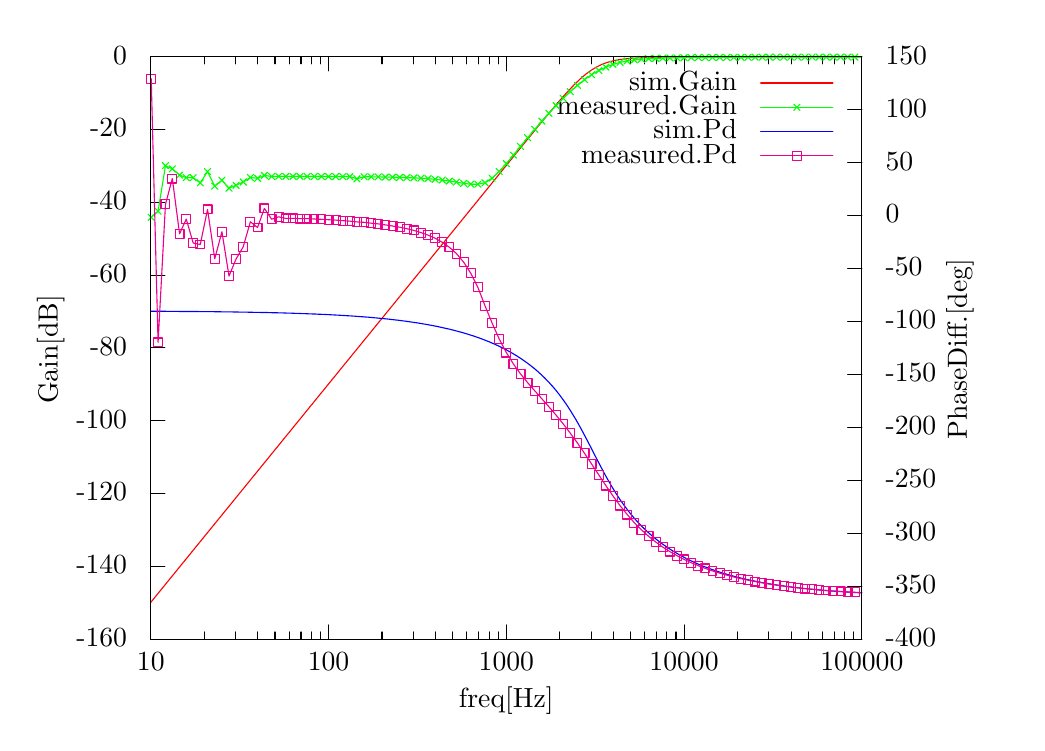
\begin{tikzpicture}[gnuplot]
%% generated with GNUPLOT 4.6p4 (Lua 5.1; terminal rev. 99, script rev. 100)
%% 2016年06月18日 10時13分38秒
\path (0.000,0.000) rectangle (12.500,8.750);
\gpcolor{color=gp lt color border}
\gpsetlinetype{gp lt border}
\gpsetlinewidth{1.00}
\draw[gp path] (1.504,0.985)--(1.684,0.985);
\node[gp node right] at (1.320,0.985) {-160};
\draw[gp path] (1.504,1.910)--(1.684,1.910);
\node[gp node right] at (1.320,1.910) {-140};
\draw[gp path] (1.504,2.834)--(1.684,2.834);
\node[gp node right] at (1.320,2.834) {-120};
\draw[gp path] (1.504,3.759)--(1.684,3.759);
\node[gp node right] at (1.320,3.759) {-100};
\draw[gp path] (1.504,4.683)--(1.684,4.683);
\node[gp node right] at (1.320,4.683) {-80};
\draw[gp path] (1.504,5.608)--(1.684,5.608);
\node[gp node right] at (1.320,5.608) {-60};
\draw[gp path] (1.504,6.532)--(1.684,6.532);
\node[gp node right] at (1.320,6.532) {-40};
\draw[gp path] (1.504,7.457)--(1.684,7.457);
\node[gp node right] at (1.320,7.457) {-20};
\draw[gp path] (1.504,8.381)--(1.684,8.381);
\node[gp node right] at (1.320,8.381) { 0};
\draw[gp path] (1.504,0.985)--(1.504,1.165);
\draw[gp path] (1.504,8.381)--(1.504,8.201);
\node[gp node center] at (1.504,0.677) { 10};
\draw[gp path] (2.184,0.985)--(2.184,1.075);
\draw[gp path] (2.184,8.381)--(2.184,8.291);
\draw[gp path] (2.581,0.985)--(2.581,1.075);
\draw[gp path] (2.581,8.381)--(2.581,8.291);
\draw[gp path] (2.863,0.985)--(2.863,1.075);
\draw[gp path] (2.863,8.381)--(2.863,8.291);
\draw[gp path] (3.082,0.985)--(3.082,1.075);
\draw[gp path] (3.082,8.381)--(3.082,8.291);
\draw[gp path] (3.261,0.985)--(3.261,1.075);
\draw[gp path] (3.261,8.381)--(3.261,8.291);
\draw[gp path] (3.412,0.985)--(3.412,1.075);
\draw[gp path] (3.412,8.381)--(3.412,8.291);
\draw[gp path] (3.543,0.985)--(3.543,1.075);
\draw[gp path] (3.543,8.381)--(3.543,8.291);
\draw[gp path] (3.658,0.985)--(3.658,1.075);
\draw[gp path] (3.658,8.381)--(3.658,8.291);
\draw[gp path] (3.762,0.985)--(3.762,1.165);
\draw[gp path] (3.762,8.381)--(3.762,8.201);
\node[gp node center] at (3.762,0.677) { 100};
\draw[gp path] (4.441,0.985)--(4.441,1.075);
\draw[gp path] (4.441,8.381)--(4.441,8.291);
\draw[gp path] (4.839,0.985)--(4.839,1.075);
\draw[gp path] (4.839,8.381)--(4.839,8.291);
\draw[gp path] (5.121,0.985)--(5.121,1.075);
\draw[gp path] (5.121,8.381)--(5.121,8.291);
\draw[gp path] (5.340,0.985)--(5.340,1.075);
\draw[gp path] (5.340,8.381)--(5.340,8.291);
\draw[gp path] (5.519,0.985)--(5.519,1.075);
\draw[gp path] (5.519,8.381)--(5.519,8.291);
\draw[gp path] (5.670,0.985)--(5.670,1.075);
\draw[gp path] (5.670,8.381)--(5.670,8.291);
\draw[gp path] (5.801,0.985)--(5.801,1.075);
\draw[gp path] (5.801,8.381)--(5.801,8.291);
\draw[gp path] (5.916,0.985)--(5.916,1.075);
\draw[gp path] (5.916,8.381)--(5.916,8.291);
\draw[gp path] (6.020,0.985)--(6.020,1.165);
\draw[gp path] (6.020,8.381)--(6.020,8.201);
\node[gp node center] at (6.020,0.677) { 1000};
\draw[gp path] (6.699,0.985)--(6.699,1.075);
\draw[gp path] (6.699,8.381)--(6.699,8.291);
\draw[gp path] (7.097,0.985)--(7.097,1.075);
\draw[gp path] (7.097,8.381)--(7.097,8.291);
\draw[gp path] (7.379,0.985)--(7.379,1.075);
\draw[gp path] (7.379,8.381)--(7.379,8.291);
\draw[gp path] (7.598,0.985)--(7.598,1.075);
\draw[gp path] (7.598,8.381)--(7.598,8.291);
\draw[gp path] (7.776,0.985)--(7.776,1.075);
\draw[gp path] (7.776,8.381)--(7.776,8.291);
\draw[gp path] (7.928,0.985)--(7.928,1.075);
\draw[gp path] (7.928,8.381)--(7.928,8.291);
\draw[gp path] (8.058,0.985)--(8.058,1.075);
\draw[gp path] (8.058,8.381)--(8.058,8.291);
\draw[gp path] (8.174,0.985)--(8.174,1.075);
\draw[gp path] (8.174,8.381)--(8.174,8.291);
\draw[gp path] (8.277,0.985)--(8.277,1.165);
\draw[gp path] (8.277,8.381)--(8.277,8.201);
\node[gp node center] at (8.277,0.677) { 10000};
\draw[gp path] (8.957,0.985)--(8.957,1.075);
\draw[gp path] (8.957,8.381)--(8.957,8.291);
\draw[gp path] (9.354,0.985)--(9.354,1.075);
\draw[gp path] (9.354,8.381)--(9.354,8.291);
\draw[gp path] (9.637,0.985)--(9.637,1.075);
\draw[gp path] (9.637,8.381)--(9.637,8.291);
\draw[gp path] (9.855,0.985)--(9.855,1.075);
\draw[gp path] (9.855,8.381)--(9.855,8.291);
\draw[gp path] (10.034,0.985)--(10.034,1.075);
\draw[gp path] (10.034,8.381)--(10.034,8.291);
\draw[gp path] (10.185,0.985)--(10.185,1.075);
\draw[gp path] (10.185,8.381)--(10.185,8.291);
\draw[gp path] (10.316,0.985)--(10.316,1.075);
\draw[gp path] (10.316,8.381)--(10.316,8.291);
\draw[gp path] (10.432,0.985)--(10.432,1.075);
\draw[gp path] (10.432,8.381)--(10.432,8.291);
\draw[gp path] (10.535,0.985)--(10.535,1.165);
\draw[gp path] (10.535,8.381)--(10.535,8.201);
\node[gp node center] at (10.535,0.677) { 100000};
\draw[gp path] (10.535,0.985)--(10.355,0.985);
\node[gp node left] at (10.719,0.985) {-400};
\draw[gp path] (10.535,1.657)--(10.355,1.657);
\node[gp node left] at (10.719,1.657) {-350};
\draw[gp path] (10.535,2.330)--(10.355,2.330);
\node[gp node left] at (10.719,2.330) {-300};
\draw[gp path] (10.535,3.002)--(10.355,3.002);
\node[gp node left] at (10.719,3.002) {-250};
\draw[gp path] (10.535,3.674)--(10.355,3.674);
\node[gp node left] at (10.719,3.674) {-200};
\draw[gp path] (10.535,4.347)--(10.355,4.347);
\node[gp node left] at (10.719,4.347) {-150};
\draw[gp path] (10.535,5.019)--(10.355,5.019);
\node[gp node left] at (10.719,5.019) {-100};
\draw[gp path] (10.535,5.692)--(10.355,5.692);
\node[gp node left] at (10.719,5.692) {-50};
\draw[gp path] (10.535,6.364)--(10.355,6.364);
\node[gp node left] at (10.719,6.364) { 0};
\draw[gp path] (10.535,7.036)--(10.355,7.036);
\node[gp node left] at (10.719,7.036) { 50};
\draw[gp path] (10.535,7.709)--(10.355,7.709);
\node[gp node left] at (10.719,7.709) { 100};
\draw[gp path] (10.535,8.381)--(10.355,8.381);
\node[gp node left] at (10.719,8.381) { 150};
\draw[gp path] (1.504,8.381)--(1.504,0.985)--(10.535,0.985)--(10.535,8.381)--cycle;
\node[gp node center,rotate=-270] at (0.246,4.683) {Gain[dB]};
\node[gp node center,rotate=-270] at (11.792,4.683) {PhaseDiff.[deg]};
\node[gp node center] at (6.019,0.215) {freq[Hz]};
\node[gp node right] at (9.067,8.047) {sim.Gain};
\gpcolor{color=gp lt color 0}
\gpsetlinetype{gp lt plot 0}
\draw[gp path] (9.251,8.047)--(10.167,8.047);
\draw[gp path] (1.504,1.451)--(1.509,1.457)--(1.513,1.462)--(1.518,1.468)--(1.522,1.473)%
  --(1.527,1.479)--(1.531,1.484)--(1.536,1.490)--(1.540,1.495)--(1.545,1.501)--(1.549,1.507)%
  --(1.554,1.512)--(1.558,1.518)--(1.563,1.523)--(1.567,1.529)--(1.572,1.534)--(1.576,1.540)%
  --(1.581,1.545)--(1.585,1.551)--(1.590,1.556)--(1.594,1.562)--(1.599,1.568)--(1.603,1.573)%
  --(1.608,1.579)--(1.612,1.584)--(1.617,1.590)--(1.621,1.595)--(1.626,1.601)--(1.630,1.606)%
  --(1.635,1.612)--(1.639,1.617)--(1.644,1.623)--(1.648,1.629)--(1.653,1.634)--(1.658,1.640)%
  --(1.662,1.645)--(1.667,1.651)--(1.671,1.656)--(1.676,1.662)--(1.680,1.667)--(1.685,1.673)%
  --(1.689,1.678)--(1.694,1.684)--(1.698,1.690)--(1.703,1.695)--(1.707,1.701)--(1.712,1.706)%
  --(1.716,1.712)--(1.721,1.717)--(1.725,1.723)--(1.730,1.728)--(1.734,1.734)--(1.739,1.740)%
  --(1.743,1.745)--(1.748,1.751)--(1.752,1.756)--(1.757,1.762)--(1.761,1.767)--(1.766,1.773)%
  --(1.770,1.778)--(1.775,1.784)--(1.779,1.789)--(1.784,1.795)--(1.788,1.801)--(1.793,1.806)%
  --(1.798,1.812)--(1.802,1.817)--(1.807,1.823)--(1.811,1.828)--(1.816,1.834)--(1.820,1.839)%
  --(1.825,1.845)--(1.829,1.850)--(1.834,1.856)--(1.838,1.862)--(1.843,1.867)--(1.847,1.873)%
  --(1.852,1.878)--(1.856,1.884)--(1.861,1.889)--(1.865,1.895)--(1.870,1.900)--(1.874,1.906)%
  --(1.879,1.911)--(1.883,1.917)--(1.888,1.923)--(1.892,1.928)--(1.897,1.934)--(1.901,1.939)%
  --(1.906,1.945)--(1.910,1.950)--(1.915,1.956)--(1.919,1.961)--(1.924,1.967)--(1.928,1.972)%
  --(1.933,1.978)--(1.937,1.984)--(1.942,1.989)--(1.947,1.995)--(1.951,2.000)--(1.956,2.006)%
  --(1.960,2.011)--(1.965,2.017)--(1.969,2.022)--(1.974,2.028)--(1.978,2.033)--(1.983,2.039)%
  --(1.987,2.045)--(1.992,2.050)--(1.996,2.056)--(2.001,2.061)--(2.005,2.067)--(2.010,2.072)%
  --(2.014,2.078)--(2.019,2.083)--(2.023,2.089)--(2.028,2.095)--(2.032,2.100)--(2.037,2.106)%
  --(2.041,2.111)--(2.046,2.117)--(2.050,2.122)--(2.055,2.128)--(2.059,2.133)--(2.064,2.139)%
  --(2.068,2.144)--(2.073,2.150)--(2.077,2.156)--(2.082,2.161)--(2.086,2.167)--(2.091,2.172)%
  --(2.096,2.178)--(2.100,2.183)--(2.105,2.189)--(2.109,2.194)--(2.114,2.200)--(2.118,2.205)%
  --(2.123,2.211)--(2.127,2.217)--(2.132,2.222)--(2.136,2.228)--(2.141,2.233)--(2.145,2.239)%
  --(2.150,2.244)--(2.154,2.250)--(2.159,2.255)--(2.163,2.261)--(2.168,2.266)--(2.172,2.272)%
  --(2.177,2.278)--(2.181,2.283)--(2.186,2.289)--(2.190,2.294)--(2.195,2.300)--(2.199,2.305)%
  --(2.204,2.311)--(2.208,2.316)--(2.213,2.322)--(2.217,2.327)--(2.222,2.333)--(2.226,2.339)%
  --(2.231,2.344)--(2.236,2.350)--(2.240,2.355)--(2.245,2.361)--(2.249,2.366)--(2.254,2.372)%
  --(2.258,2.377)--(2.263,2.383)--(2.267,2.389)--(2.272,2.394)--(2.276,2.400)--(2.281,2.405)%
  --(2.285,2.411)--(2.290,2.416)--(2.294,2.422)--(2.299,2.427)--(2.303,2.433)--(2.308,2.438)%
  --(2.312,2.444)--(2.317,2.450)--(2.321,2.455)--(2.326,2.461)--(2.330,2.466)--(2.335,2.472)%
  --(2.339,2.477)--(2.344,2.483)--(2.348,2.488)--(2.353,2.494)--(2.357,2.499)--(2.362,2.505)%
  --(2.366,2.511)--(2.371,2.516)--(2.375,2.522)--(2.380,2.527)--(2.385,2.533)--(2.389,2.538)%
  --(2.394,2.544)--(2.398,2.549)--(2.403,2.555)--(2.407,2.560)--(2.412,2.566)--(2.416,2.572)%
  --(2.421,2.577)--(2.425,2.583)--(2.430,2.588)--(2.434,2.594)--(2.439,2.599)--(2.443,2.605)%
  --(2.448,2.610)--(2.452,2.616)--(2.457,2.621)--(2.461,2.627)--(2.466,2.633)--(2.470,2.638)%
  --(2.475,2.644)--(2.479,2.649)--(2.484,2.655)--(2.488,2.660)--(2.493,2.666)--(2.497,2.671)%
  --(2.502,2.677)--(2.506,2.682)--(2.511,2.688)--(2.515,2.694)--(2.520,2.699)--(2.525,2.705)%
  --(2.529,2.710)--(2.534,2.716)--(2.538,2.721)--(2.543,2.727)--(2.547,2.732)--(2.552,2.738)%
  --(2.556,2.744)--(2.561,2.749)--(2.565,2.755)--(2.570,2.760)--(2.574,2.766)--(2.579,2.771)%
  --(2.583,2.777)--(2.588,2.782)--(2.592,2.788)--(2.597,2.793)--(2.601,2.799)--(2.606,2.805)%
  --(2.610,2.810)--(2.615,2.816)--(2.619,2.821)--(2.624,2.827)--(2.628,2.832)--(2.633,2.838)%
  --(2.637,2.843)--(2.642,2.849)--(2.646,2.854)--(2.651,2.860)--(2.655,2.866)--(2.660,2.871)%
  --(2.664,2.877)--(2.669,2.882)--(2.674,2.888)--(2.678,2.893)--(2.683,2.899)--(2.687,2.904)%
  --(2.692,2.910)--(2.696,2.915)--(2.701,2.921)--(2.705,2.927)--(2.710,2.932)--(2.714,2.938)%
  --(2.719,2.943)--(2.723,2.949)--(2.728,2.954)--(2.732,2.960)--(2.737,2.965)--(2.741,2.971)%
  --(2.746,2.976)--(2.750,2.982)--(2.755,2.988)--(2.759,2.993)--(2.764,2.999)--(2.768,3.004)%
  --(2.773,3.010)--(2.777,3.015)--(2.782,3.021)--(2.786,3.026)--(2.791,3.032)--(2.795,3.038)%
  --(2.800,3.043)--(2.804,3.049)--(2.809,3.054)--(2.813,3.060)--(2.818,3.065)--(2.823,3.071)%
  --(2.827,3.076)--(2.832,3.082)--(2.836,3.087)--(2.841,3.093)--(2.845,3.099)--(2.850,3.104)%
  --(2.854,3.110)--(2.859,3.115)--(2.863,3.121)--(2.868,3.126)--(2.872,3.132)--(2.877,3.137)%
  --(2.881,3.143)--(2.886,3.148)--(2.890,3.154)--(2.895,3.160)--(2.899,3.165)--(2.904,3.171)%
  --(2.908,3.176)--(2.913,3.182)--(2.917,3.187)--(2.922,3.193)--(2.926,3.198)--(2.931,3.204)%
  --(2.935,3.209)--(2.940,3.215)--(2.944,3.221)--(2.949,3.226)--(2.953,3.232)--(2.958,3.237)%
  --(2.963,3.243)--(2.967,3.248)--(2.972,3.254)--(2.976,3.259)--(2.981,3.265)--(2.985,3.270)%
  --(2.990,3.276)--(2.994,3.282)--(2.999,3.287)--(3.003,3.293)--(3.008,3.298)--(3.012,3.304)%
  --(3.017,3.309)--(3.021,3.315)--(3.026,3.320)--(3.030,3.326)--(3.035,3.331)--(3.039,3.337)%
  --(3.044,3.343)--(3.048,3.348)--(3.053,3.354)--(3.057,3.359)--(3.062,3.365)--(3.066,3.370)%
  --(3.071,3.376)--(3.075,3.381)--(3.080,3.387)--(3.084,3.393)--(3.089,3.398)--(3.093,3.404)%
  --(3.098,3.409)--(3.102,3.415)--(3.107,3.420)--(3.112,3.426)--(3.116,3.431)--(3.121,3.437)%
  --(3.125,3.442)--(3.130,3.448)--(3.134,3.454)--(3.139,3.459)--(3.143,3.465)--(3.148,3.470)%
  --(3.152,3.476)--(3.157,3.481)--(3.161,3.487)--(3.166,3.492)--(3.170,3.498)--(3.175,3.503)%
  --(3.179,3.509)--(3.184,3.515)--(3.188,3.520)--(3.193,3.526)--(3.197,3.531)--(3.202,3.537)%
  --(3.206,3.542)--(3.211,3.548)--(3.215,3.553)--(3.220,3.559)--(3.224,3.564)--(3.229,3.570)%
  --(3.233,3.576)--(3.238,3.581)--(3.242,3.587)--(3.247,3.592)--(3.251,3.598)--(3.256,3.603)%
  --(3.261,3.609)--(3.265,3.614)--(3.270,3.620)--(3.274,3.625)--(3.279,3.631)--(3.283,3.637)%
  --(3.288,3.642)--(3.292,3.648)--(3.297,3.653)--(3.301,3.659)--(3.306,3.664)--(3.310,3.670)%
  --(3.315,3.675)--(3.319,3.681)--(3.324,3.687)--(3.328,3.692)--(3.333,3.698)--(3.337,3.703)%
  --(3.342,3.709)--(3.346,3.714)--(3.351,3.720)--(3.355,3.725)--(3.360,3.731)--(3.364,3.736)%
  --(3.369,3.742)--(3.373,3.748)--(3.378,3.753)--(3.382,3.759)--(3.387,3.764)--(3.391,3.770)%
  --(3.396,3.775)--(3.401,3.781)--(3.405,3.786)--(3.410,3.792)--(3.414,3.797)--(3.419,3.803)%
  --(3.423,3.809)--(3.428,3.814)--(3.432,3.820)--(3.437,3.825)--(3.441,3.831)--(3.446,3.836)%
  --(3.450,3.842)--(3.455,3.847)--(3.459,3.853)--(3.464,3.858)--(3.468,3.864)--(3.473,3.870)%
  --(3.477,3.875)--(3.482,3.881)--(3.486,3.886)--(3.491,3.892)--(3.495,3.897)--(3.500,3.903)%
  --(3.504,3.908)--(3.509,3.914)--(3.513,3.919)--(3.518,3.925)--(3.522,3.931)--(3.527,3.936)%
  --(3.531,3.942)--(3.536,3.947)--(3.540,3.953)--(3.545,3.958)--(3.550,3.964)--(3.554,3.969)%
  --(3.559,3.975)--(3.563,3.981)--(3.568,3.986)--(3.572,3.992)--(3.577,3.997)--(3.581,4.003)%
  --(3.586,4.008)--(3.590,4.014)--(3.595,4.019)--(3.599,4.025)--(3.604,4.030)--(3.608,4.036)%
  --(3.613,4.042)--(3.617,4.047)--(3.622,4.053)--(3.626,4.058)--(3.631,4.064)--(3.635,4.069)%
  --(3.640,4.075)--(3.644,4.080)--(3.649,4.086)--(3.653,4.091)--(3.658,4.097)--(3.662,4.103)%
  --(3.667,4.108)--(3.671,4.114)--(3.676,4.119)--(3.680,4.125)--(3.685,4.130)--(3.690,4.136)%
  --(3.694,4.141)--(3.699,4.147)--(3.703,4.152)--(3.708,4.158)--(3.712,4.164)--(3.717,4.169)%
  --(3.721,4.175)--(3.726,4.180)--(3.730,4.186)--(3.735,4.191)--(3.739,4.197)--(3.744,4.202)%
  --(3.748,4.208)--(3.753,4.213)--(3.757,4.219)--(3.762,4.225)--(3.766,4.230)--(3.771,4.236)%
  --(3.775,4.241)--(3.780,4.247)--(3.784,4.252)--(3.789,4.258)--(3.793,4.263)--(3.798,4.269)%
  --(3.802,4.275)--(3.807,4.280)--(3.811,4.286)--(3.816,4.291)--(3.820,4.297)--(3.825,4.302)%
  --(3.829,4.308)--(3.834,4.313)--(3.839,4.319)--(3.843,4.324)--(3.848,4.330)--(3.852,4.336)%
  --(3.857,4.341)--(3.861,4.347)--(3.866,4.352)--(3.870,4.358)--(3.875,4.363)--(3.879,4.369)%
  --(3.884,4.374)--(3.888,4.380)--(3.893,4.385)--(3.897,4.391)--(3.902,4.397)--(3.906,4.402)%
  --(3.911,4.408)--(3.915,4.413)--(3.920,4.419)--(3.924,4.424)--(3.929,4.430)--(3.933,4.435)%
  --(3.938,4.441)--(3.942,4.446)--(3.947,4.452)--(3.951,4.458)--(3.956,4.463)--(3.960,4.469)%
  --(3.965,4.474)--(3.969,4.480)--(3.974,4.485)--(3.978,4.491)--(3.983,4.496)--(3.988,4.502)%
  --(3.992,4.508)--(3.997,4.513)--(4.001,4.519)--(4.006,4.524)--(4.010,4.530)--(4.015,4.535)%
  --(4.019,4.541)--(4.024,4.546)--(4.028,4.552)--(4.033,4.557)--(4.037,4.563)--(4.042,4.569)%
  --(4.046,4.574)--(4.051,4.580)--(4.055,4.585)--(4.060,4.591)--(4.064,4.596)--(4.069,4.602)%
  --(4.073,4.607)--(4.078,4.613)--(4.082,4.618)--(4.087,4.624)--(4.091,4.630)--(4.096,4.635)%
  --(4.100,4.641)--(4.105,4.646)--(4.109,4.652)--(4.114,4.657)--(4.118,4.663)--(4.123,4.668)%
  --(4.128,4.674)--(4.132,4.679)--(4.137,4.685)--(4.141,4.691)--(4.146,4.696)--(4.150,4.702)%
  --(4.155,4.707)--(4.159,4.713)--(4.164,4.718)--(4.168,4.724)--(4.173,4.729)--(4.177,4.735)%
  --(4.182,4.740)--(4.186,4.746)--(4.191,4.752)--(4.195,4.757)--(4.200,4.763)--(4.204,4.768)%
  --(4.209,4.774)--(4.213,4.779)--(4.218,4.785)--(4.222,4.790)--(4.227,4.796)--(4.231,4.802)%
  --(4.236,4.807)--(4.240,4.813)--(4.245,4.818)--(4.249,4.824)--(4.254,4.829)--(4.258,4.835)%
  --(4.263,4.840)--(4.267,4.846)--(4.272,4.851)--(4.277,4.857)--(4.281,4.863)--(4.286,4.868)%
  --(4.290,4.874)--(4.295,4.879)--(4.299,4.885)--(4.304,4.890)--(4.308,4.896)--(4.313,4.901)%
  --(4.317,4.907)--(4.322,4.912)--(4.326,4.918)--(4.331,4.924)--(4.335,4.929)--(4.340,4.935)%
  --(4.344,4.940)--(4.349,4.946)--(4.353,4.951)--(4.358,4.957)--(4.362,4.962)--(4.367,4.968)%
  --(4.371,4.974)--(4.376,4.979)--(4.380,4.985)--(4.385,4.990)--(4.389,4.996)--(4.394,5.001)%
  --(4.398,5.007)--(4.403,5.012)--(4.407,5.018)--(4.412,5.023)--(4.416,5.029)--(4.421,5.035)%
  --(4.426,5.040)--(4.430,5.046)--(4.435,5.051)--(4.439,5.057)--(4.444,5.062)--(4.448,5.068)%
  --(4.453,5.073)--(4.457,5.079)--(4.462,5.084)--(4.466,5.090)--(4.471,5.096)--(4.475,5.101)%
  --(4.480,5.107)--(4.484,5.112)--(4.489,5.118)--(4.493,5.123)--(4.498,5.129)--(4.502,5.134)%
  --(4.507,5.140)--(4.511,5.145)--(4.516,5.151)--(4.520,5.157)--(4.525,5.162)--(4.529,5.168)%
  --(4.534,5.173)--(4.538,5.179)--(4.543,5.184)--(4.547,5.190)--(4.552,5.195)--(4.556,5.201)%
  --(4.561,5.207)--(4.566,5.212)--(4.570,5.218)--(4.575,5.223)--(4.579,5.229)--(4.584,5.234)%
  --(4.588,5.240)--(4.593,5.245)--(4.597,5.251)--(4.602,5.256)--(4.606,5.262)--(4.611,5.268)%
  --(4.615,5.273)--(4.620,5.279)--(4.624,5.284)--(4.629,5.290)--(4.633,5.295)--(4.638,5.301)%
  --(4.642,5.306)--(4.647,5.312)--(4.651,5.317)--(4.656,5.323)--(4.660,5.329)--(4.665,5.334)%
  --(4.669,5.340)--(4.674,5.345)--(4.678,5.351)--(4.683,5.356)--(4.687,5.362)--(4.692,5.367)%
  --(4.696,5.373)--(4.701,5.379)--(4.705,5.384)--(4.710,5.390)--(4.715,5.395)--(4.719,5.401)%
  --(4.724,5.406)--(4.728,5.412)--(4.733,5.417)--(4.737,5.423)--(4.742,5.428)--(4.746,5.434)%
  --(4.751,5.440)--(4.755,5.445)--(4.760,5.451)--(4.764,5.456)--(4.769,5.462)--(4.773,5.467)%
  --(4.778,5.473)--(4.782,5.478)--(4.787,5.484)--(4.791,5.490)--(4.796,5.495)--(4.800,5.501)%
  --(4.805,5.506)--(4.809,5.512)--(4.814,5.517)--(4.818,5.523)--(4.823,5.528)--(4.827,5.534)%
  --(4.832,5.539)--(4.836,5.545)--(4.841,5.551)--(4.845,5.556)--(4.850,5.562)--(4.855,5.567)%
  --(4.859,5.573)--(4.864,5.578)--(4.868,5.584)--(4.873,5.589)--(4.877,5.595)--(4.882,5.601)%
  --(4.886,5.606)--(4.891,5.612)--(4.895,5.617)--(4.900,5.623)--(4.904,5.628)--(4.909,5.634)%
  --(4.913,5.639)--(4.918,5.645)--(4.922,5.650)--(4.927,5.656)--(4.931,5.662)--(4.936,5.667)%
  --(4.940,5.673)--(4.945,5.678)--(4.949,5.684)--(4.954,5.689)--(4.958,5.695)--(4.963,5.700)%
  --(4.967,5.706)--(4.972,5.711)--(4.976,5.717)--(4.981,5.723)--(4.985,5.728)--(4.990,5.734)%
  --(4.994,5.739)--(4.999,5.745)--(5.004,5.750)--(5.008,5.756)--(5.013,5.761)--(5.017,5.767)%
  --(5.022,5.773)--(5.026,5.778)--(5.031,5.784)--(5.035,5.789)--(5.040,5.795)--(5.044,5.800)%
  --(5.049,5.806)--(5.053,5.811)--(5.058,5.817)--(5.062,5.823)--(5.067,5.828)--(5.071,5.834)%
  --(5.076,5.839)--(5.080,5.845)--(5.085,5.850)--(5.089,5.856)--(5.094,5.861)--(5.098,5.867)%
  --(5.103,5.872)--(5.107,5.878)--(5.112,5.884)--(5.116,5.889)--(5.121,5.895)--(5.125,5.900)%
  --(5.130,5.906)--(5.134,5.911)--(5.139,5.917)--(5.143,5.922)--(5.148,5.928)--(5.153,5.934)%
  --(5.157,5.939)--(5.162,5.945)--(5.166,5.950)--(5.171,5.956)--(5.175,5.961)--(5.180,5.967)%
  --(5.184,5.972)--(5.189,5.978)--(5.193,5.983)--(5.198,5.989)--(5.202,5.995)--(5.207,6.000)%
  --(5.211,6.006)--(5.216,6.011)--(5.220,6.017)--(5.225,6.022)--(5.229,6.028)--(5.234,6.033)%
  --(5.238,6.039)--(5.243,6.045)--(5.247,6.050)--(5.252,6.056)--(5.256,6.061)--(5.261,6.067)%
  --(5.265,6.072)--(5.270,6.078)--(5.274,6.083)--(5.279,6.089)--(5.283,6.095)--(5.288,6.100)%
  --(5.293,6.106)--(5.297,6.111)--(5.302,6.117)--(5.306,6.122)--(5.311,6.128)--(5.315,6.133)%
  --(5.320,6.139)--(5.324,6.145)--(5.329,6.150)--(5.333,6.156)--(5.338,6.161)--(5.342,6.167)%
  --(5.347,6.172)--(5.351,6.178)--(5.356,6.183)--(5.360,6.189)--(5.365,6.194)--(5.369,6.200)%
  --(5.374,6.206)--(5.378,6.211)--(5.383,6.217)--(5.387,6.222)--(5.392,6.228)--(5.396,6.233)%
  --(5.401,6.239)--(5.405,6.244)--(5.410,6.250)--(5.414,6.256)--(5.419,6.261)--(5.423,6.267)%
  --(5.428,6.272)--(5.432,6.278)--(5.437,6.283)--(5.442,6.289)--(5.446,6.294)--(5.451,6.300)%
  --(5.455,6.306)--(5.460,6.311)--(5.464,6.317)--(5.469,6.322)--(5.473,6.328)--(5.478,6.333)%
  --(5.482,6.339)--(5.487,6.344)--(5.491,6.350)--(5.496,6.356)--(5.500,6.361)--(5.505,6.367)%
  --(5.509,6.372)--(5.514,6.378)--(5.518,6.383)--(5.523,6.389)--(5.527,6.394)--(5.532,6.400)%
  --(5.536,6.406)--(5.541,6.411)--(5.545,6.417)--(5.550,6.422)--(5.554,6.428)--(5.559,6.433)%
  --(5.563,6.439)--(5.568,6.444)--(5.572,6.450)--(5.577,6.456)--(5.581,6.461)--(5.586,6.467)%
  --(5.591,6.472)--(5.595,6.478)--(5.600,6.483)--(5.604,6.489)--(5.609,6.494)--(5.613,6.500)%
  --(5.618,6.506)--(5.622,6.511)--(5.627,6.517)--(5.631,6.522)--(5.636,6.528)--(5.640,6.533)%
  --(5.645,6.539)--(5.649,6.544)--(5.654,6.550)--(5.658,6.556)--(5.663,6.561)--(5.667,6.567)%
  --(5.672,6.572)--(5.676,6.578)--(5.681,6.583)--(5.685,6.589)--(5.690,6.595)--(5.694,6.600)%
  --(5.699,6.606)--(5.703,6.611)--(5.708,6.617)--(5.712,6.622)--(5.717,6.628)--(5.721,6.633)%
  --(5.726,6.639)--(5.731,6.645)--(5.735,6.650)--(5.740,6.656)--(5.744,6.661)--(5.749,6.667)%
  --(5.753,6.672)--(5.758,6.678)--(5.762,6.683)--(5.767,6.689)--(5.771,6.695)--(5.776,6.700)%
  --(5.780,6.706)--(5.785,6.711)--(5.789,6.717)--(5.794,6.722)--(5.798,6.728)--(5.803,6.734)%
  --(5.807,6.739)--(5.812,6.745)--(5.816,6.750)--(5.821,6.756)--(5.825,6.761)--(5.830,6.767)%
  --(5.834,6.772)--(5.839,6.778)--(5.843,6.784)--(5.848,6.789)--(5.852,6.795)--(5.857,6.800)%
  --(5.861,6.806)--(5.866,6.811)--(5.870,6.817)--(5.875,6.822)--(5.880,6.828)--(5.884,6.834)%
  --(5.889,6.839)--(5.893,6.845)--(5.898,6.850)--(5.902,6.856)--(5.907,6.861)--(5.911,6.867)%
  --(5.916,6.873)--(5.920,6.878)--(5.925,6.884)--(5.929,6.889)--(5.934,6.895)--(5.938,6.900)%
  --(5.943,6.906)--(5.947,6.911)--(5.952,6.917)--(5.956,6.923)--(5.961,6.928)--(5.965,6.934)%
  --(5.970,6.939)--(5.974,6.945)--(5.979,6.950)--(5.983,6.956)--(5.988,6.962)--(5.992,6.967)%
  --(5.997,6.973)--(6.001,6.978)--(6.006,6.984)--(6.010,6.989)--(6.015,6.995)--(6.020,7.000)%
  --(6.024,7.006)--(6.029,7.012)--(6.033,7.017)--(6.038,7.023)--(6.042,7.028)--(6.047,7.034)%
  --(6.051,7.039)--(6.056,7.045)--(6.060,7.051)--(6.065,7.056)--(6.069,7.062)--(6.074,7.067)%
  --(6.078,7.073)--(6.083,7.078)--(6.087,7.084)--(6.092,7.089)--(6.096,7.095)--(6.101,7.101)%
  --(6.105,7.106)--(6.110,7.112)--(6.114,7.117)--(6.119,7.123)--(6.123,7.128)--(6.128,7.134)%
  --(6.132,7.139)--(6.137,7.145)--(6.141,7.151)--(6.146,7.156)--(6.150,7.162)--(6.155,7.167)%
  --(6.159,7.173)--(6.164,7.178)--(6.169,7.184)--(6.173,7.190)--(6.178,7.195)--(6.182,7.201)%
  --(6.187,7.206)--(6.191,7.212)--(6.196,7.217)--(6.200,7.223)--(6.205,7.228)--(6.209,7.234)%
  --(6.214,7.240)--(6.218,7.245)--(6.223,7.251)--(6.227,7.256)--(6.232,7.262)--(6.236,7.267)%
  --(6.241,7.273)--(6.245,7.278)--(6.250,7.284)--(6.254,7.289)--(6.259,7.295)--(6.263,7.301)%
  --(6.268,7.306)--(6.272,7.312)--(6.277,7.317)--(6.281,7.323)--(6.286,7.328)--(6.290,7.334)%
  --(6.295,7.339)--(6.299,7.345)--(6.304,7.351)--(6.308,7.356)--(6.313,7.362)--(6.318,7.367)%
  --(6.322,7.373)--(6.327,7.378)--(6.331,7.384)--(6.336,7.389)--(6.340,7.395)--(6.345,7.400)%
  --(6.349,7.406)--(6.354,7.411)--(6.358,7.417)--(6.363,7.422)--(6.367,7.428)--(6.372,7.434)%
  --(6.376,7.439)--(6.381,7.445)--(6.385,7.450)--(6.390,7.456)--(6.394,7.461)--(6.399,7.467)%
  --(6.403,7.472)--(6.408,7.478)--(6.412,7.483)--(6.417,7.489)--(6.421,7.494)--(6.426,7.500)%
  --(6.430,7.505)--(6.435,7.511)--(6.439,7.516)--(6.444,7.522)--(6.448,7.527)--(6.453,7.533)%
  --(6.458,7.538)--(6.462,7.544)--(6.467,7.549)--(6.471,7.555)--(6.476,7.560)--(6.480,7.566)%
  --(6.485,7.571)--(6.489,7.577)--(6.494,7.582)--(6.498,7.588)--(6.503,7.593)--(6.507,7.598)%
  --(6.512,7.604)--(6.516,7.609)--(6.521,7.615)--(6.525,7.620)--(6.530,7.626)--(6.534,7.631)%
  --(6.539,7.637)--(6.543,7.642)--(6.548,7.647)--(6.552,7.653)--(6.557,7.658)--(6.561,7.664)%
  --(6.566,7.669)--(6.570,7.675)--(6.575,7.680)--(6.579,7.685)--(6.584,7.691)--(6.588,7.696)%
  --(6.593,7.701)--(6.597,7.707)--(6.602,7.712)--(6.607,7.718)--(6.611,7.723)--(6.616,7.728)%
  --(6.620,7.734)--(6.625,7.739)--(6.629,7.744)--(6.634,7.750)--(6.638,7.755)--(6.643,7.760)%
  --(6.647,7.766)--(6.652,7.771)--(6.656,7.776)--(6.661,7.781)--(6.665,7.787)--(6.670,7.792)%
  --(6.674,7.797)--(6.679,7.802)--(6.683,7.808)--(6.688,7.813)--(6.692,7.818)--(6.697,7.823)%
  --(6.701,7.829)--(6.706,7.834)--(6.710,7.839)--(6.715,7.844)--(6.719,7.849)--(6.724,7.854)%
  --(6.728,7.860)--(6.733,7.865)--(6.737,7.870)--(6.742,7.875)--(6.746,7.880)--(6.751,7.885)%
  --(6.756,7.890)--(6.760,7.895)--(6.765,7.900)--(6.769,7.905)--(6.774,7.910)--(6.778,7.915)%
  --(6.783,7.920)--(6.787,7.925)--(6.792,7.930)--(6.796,7.935)--(6.801,7.940)--(6.805,7.945)%
  --(6.810,7.950)--(6.814,7.955)--(6.819,7.959)--(6.823,7.964)--(6.828,7.969)--(6.832,7.974)%
  --(6.837,7.979)--(6.841,7.983)--(6.846,7.988)--(6.850,7.993)--(6.855,7.997)--(6.859,8.002)%
  --(6.864,8.007)--(6.868,8.011)--(6.873,8.016)--(6.877,8.021)--(6.882,8.025)--(6.886,8.030)%
  --(6.891,8.034)--(6.896,8.039)--(6.900,8.043)--(6.905,8.048)--(6.909,8.052)--(6.914,8.056)%
  --(6.918,8.061)--(6.923,8.065)--(6.927,8.069)--(6.932,8.074)--(6.936,8.078)--(6.941,8.082)%
  --(6.945,8.086)--(6.950,8.090)--(6.954,8.095)--(6.959,8.099)--(6.963,8.103)--(6.968,8.107)%
  --(6.972,8.111)--(6.977,8.115)--(6.981,8.119)--(6.986,8.123)--(6.990,8.127)--(6.995,8.130)%
  --(6.999,8.134)--(7.004,8.138)--(7.008,8.142)--(7.013,8.146)--(7.017,8.149)--(7.022,8.153)%
  --(7.026,8.157)--(7.031,8.160)--(7.035,8.164)--(7.040,8.167)--(7.045,8.171)--(7.049,8.174)%
  --(7.054,8.177)--(7.058,8.181)--(7.063,8.184)--(7.067,8.187)--(7.072,8.191)--(7.076,8.194)%
  --(7.081,8.197)--(7.085,8.200)--(7.090,8.203)--(7.094,8.206)--(7.099,8.210)--(7.103,8.213)%
  --(7.108,8.215)--(7.112,8.218)--(7.117,8.221)--(7.121,8.224)--(7.126,8.227)--(7.130,8.230)%
  --(7.135,8.232)--(7.139,8.235)--(7.144,8.238)--(7.148,8.240)--(7.153,8.243)--(7.157,8.246)%
  --(7.162,8.248)--(7.166,8.250)--(7.171,8.253)--(7.175,8.255)--(7.180,8.258)--(7.184,8.260)%
  --(7.189,8.262)--(7.194,8.265)--(7.198,8.267)--(7.203,8.269)--(7.207,8.271)--(7.212,8.273)%
  --(7.216,8.275)--(7.221,8.277)--(7.225,8.279)--(7.230,8.281)--(7.234,8.283)--(7.239,8.285)%
  --(7.243,8.287)--(7.248,8.289)--(7.252,8.291)--(7.257,8.292)--(7.261,8.294)--(7.266,8.296)%
  --(7.270,8.297)--(7.275,8.299)--(7.279,8.301)--(7.284,8.302)--(7.288,8.304)--(7.293,8.305)%
  --(7.297,8.307)--(7.302,8.308)--(7.306,8.310)--(7.311,8.311)--(7.315,8.313)--(7.320,8.314)%
  --(7.324,8.315)--(7.329,8.317)--(7.334,8.318)--(7.338,8.319)--(7.343,8.320)--(7.347,8.321)%
  --(7.352,8.323)--(7.356,8.324)--(7.361,8.325)--(7.365,8.326)--(7.370,8.327)--(7.374,8.328)%
  --(7.379,8.329)--(7.383,8.330)--(7.388,8.331)--(7.392,8.332)--(7.397,8.333)--(7.401,8.334)%
  --(7.406,8.335)--(7.410,8.336)--(7.415,8.337)--(7.419,8.338)--(7.424,8.338)--(7.428,8.339)%
  --(7.433,8.340)--(7.437,8.341)--(7.442,8.342)--(7.446,8.342)--(7.451,8.343)--(7.455,8.344)%
  --(7.460,8.344)--(7.464,8.345)--(7.469,8.346)--(7.473,8.346)--(7.478,8.347)--(7.483,8.348)%
  --(7.487,8.348)--(7.492,8.349)--(7.496,8.350)--(7.501,8.350)--(7.505,8.351)--(7.510,8.351)%
  --(7.514,8.352)--(7.519,8.352)--(7.523,8.353)--(7.528,8.353)--(7.532,8.354)--(7.537,8.354)%
  --(7.541,8.355)--(7.546,8.355)--(7.550,8.356)--(7.555,8.356)--(7.559,8.357)--(7.564,8.357)%
  --(7.568,8.357)--(7.573,8.358)--(7.577,8.358)--(7.582,8.359)--(7.586,8.359)--(7.591,8.359)%
  --(7.595,8.360)--(7.600,8.360)--(7.604,8.360)--(7.609,8.361)--(7.613,8.361)--(7.618,8.361)%
  --(7.623,8.362)--(7.627,8.362)--(7.632,8.362)--(7.636,8.363)--(7.641,8.363)--(7.645,8.363)%
  --(7.650,8.364)--(7.654,8.364)--(7.659,8.364)--(7.663,8.364)--(7.668,8.365)--(7.672,8.365)%
  --(7.677,8.365)--(7.681,8.365)--(7.686,8.366)--(7.690,8.366)--(7.695,8.366)--(7.699,8.366)%
  --(7.704,8.366)--(7.708,8.367)--(7.713,8.367)--(7.717,8.367)--(7.722,8.367)--(7.726,8.367)%
  --(7.731,8.368)--(7.735,8.368)--(7.740,8.368)--(7.744,8.368)--(7.749,8.368)--(7.753,8.369)%
  --(7.758,8.369)--(7.762,8.369)--(7.767,8.369)--(7.772,8.369)--(7.776,8.369)--(7.781,8.370)%
  --(7.785,8.370)--(7.790,8.370)--(7.794,8.370)--(7.799,8.370)--(7.803,8.370)--(7.808,8.370)%
  --(7.812,8.371)--(7.817,8.371)--(7.821,8.371)--(7.826,8.371)--(7.830,8.371)--(7.835,8.371)%
  --(7.839,8.371)--(7.844,8.371)--(7.848,8.372)--(7.853,8.372)--(7.857,8.372)--(7.862,8.372)%
  --(7.866,8.372)--(7.871,8.372)--(7.875,8.372)--(7.880,8.372)--(7.884,8.372)--(7.889,8.373)%
  --(7.893,8.373)--(7.898,8.373)--(7.902,8.373)--(7.907,8.373)--(7.911,8.373)--(7.916,8.373)%
  --(7.921,8.373)--(7.925,8.373)--(7.930,8.373)--(7.934,8.374)--(7.939,8.374)--(7.943,8.374)%
  --(7.948,8.374)--(7.952,8.374)--(7.957,8.374)--(7.961,8.374)--(7.966,8.374)--(7.970,8.374)%
  --(7.975,8.374)--(7.979,8.374)--(7.984,8.374)--(7.988,8.374)--(7.993,8.375)--(7.997,8.375)%
  --(8.002,8.375)--(8.006,8.375)--(8.011,8.375)--(8.015,8.375)--(8.020,8.375)--(8.024,8.375)%
  --(8.029,8.375)--(8.033,8.375)--(8.038,8.375)--(8.042,8.375)--(8.047,8.375)--(8.051,8.375)%
  --(8.056,8.375)--(8.061,8.375)--(8.065,8.376)--(8.070,8.376)--(8.074,8.376)--(8.079,8.376)%
  --(8.083,8.376)--(8.088,8.376)--(8.092,8.376)--(8.097,8.376)--(8.101,8.376)--(8.106,8.376)%
  --(8.110,8.376)--(8.115,8.376)--(8.119,8.376)--(8.124,8.376)--(8.128,8.376)--(8.133,8.376)%
  --(8.137,8.376)--(8.142,8.376)--(8.146,8.376)--(8.151,8.376)--(8.155,8.377)--(8.160,8.377)%
  --(8.164,8.377)--(8.169,8.377)--(8.173,8.377)--(8.178,8.377)--(8.182,8.377)--(8.187,8.377)%
  --(8.191,8.377)--(8.196,8.377)--(8.200,8.377)--(8.205,8.377)--(8.210,8.377)--(8.214,8.377)%
  --(8.219,8.377)--(8.223,8.377)--(8.228,8.377)--(8.232,8.377)--(8.237,8.377)--(8.241,8.377)%
  --(8.246,8.377)--(8.250,8.377)--(8.255,8.377)--(8.259,8.377)--(8.264,8.377)--(8.268,8.377)%
  --(8.273,8.378)--(8.277,8.378)--(8.282,8.378)--(8.286,8.378)--(8.291,8.378)--(8.295,8.378)%
  --(8.300,8.378)--(8.304,8.378)--(8.309,8.378)--(8.313,8.378)--(8.318,8.378)--(8.322,8.378)%
  --(8.327,8.378)--(8.331,8.378)--(8.336,8.378)--(8.340,8.378)--(8.345,8.378)--(8.349,8.378)%
  --(8.354,8.378)--(8.359,8.378)--(8.363,8.378)--(8.368,8.378)--(8.372,8.378)--(8.377,8.378)%
  --(8.381,8.378)--(8.386,8.378)--(8.390,8.378)--(8.395,8.378)--(8.399,8.378)--(8.404,8.378)%
  --(8.408,8.378)--(8.413,8.378)--(8.417,8.378)--(8.422,8.378)--(8.426,8.378)--(8.431,8.378)%
  --(8.435,8.379)--(8.440,8.379)--(8.444,8.379)--(8.449,8.379)--(8.453,8.379)--(8.458,8.379)%
  --(8.462,8.379)--(8.467,8.379)--(8.471,8.379)--(8.476,8.379)--(8.480,8.379)--(8.485,8.379)%
  --(8.489,8.379)--(8.494,8.379)--(8.499,8.379)--(8.503,8.379)--(8.508,8.379)--(8.512,8.379)%
  --(8.517,8.379)--(8.521,8.379)--(8.526,8.379)--(8.530,8.379)--(8.535,8.379)--(8.539,8.379)%
  --(8.544,8.379)--(8.548,8.379)--(8.553,8.379)--(8.557,8.379)--(8.562,8.379)--(8.566,8.379)%
  --(8.571,8.379)--(8.575,8.379)--(8.580,8.379)--(8.584,8.379)--(8.589,8.379)--(8.593,8.379)%
  --(8.598,8.379)--(8.602,8.379)--(8.607,8.379)--(8.611,8.379)--(8.616,8.379)--(8.620,8.379)%
  --(8.625,8.379)--(8.629,8.379)--(8.634,8.379)--(8.638,8.379)--(8.643,8.379)--(8.648,8.379)%
  --(8.652,8.379)--(8.657,8.379)--(8.661,8.379)--(8.666,8.379)--(8.670,8.379)--(8.675,8.379)%
  --(8.679,8.379)--(8.684,8.379)--(8.688,8.379)--(8.693,8.380)--(8.697,8.380)--(8.702,8.380)%
  --(8.706,8.380)--(8.711,8.380)--(8.715,8.380)--(8.720,8.380)--(8.724,8.380)--(8.729,8.380)%
  --(8.733,8.380)--(8.738,8.380)--(8.742,8.380)--(8.747,8.380)--(8.751,8.380)--(8.756,8.380)%
  --(8.760,8.380)--(8.765,8.380)--(8.769,8.380)--(8.774,8.380)--(8.778,8.380)--(8.783,8.380)%
  --(8.788,8.380)--(8.792,8.380)--(8.797,8.380)--(8.801,8.380)--(8.806,8.380)--(8.810,8.380)%
  --(8.815,8.380)--(8.819,8.380)--(8.824,8.380)--(8.828,8.380)--(8.833,8.380)--(8.837,8.380)%
  --(8.842,8.380)--(8.846,8.380)--(8.851,8.380)--(8.855,8.380)--(8.860,8.380)--(8.864,8.380)%
  --(8.869,8.380)--(8.873,8.380)--(8.878,8.380)--(8.882,8.380)--(8.887,8.380)--(8.891,8.380)%
  --(8.896,8.380)--(8.900,8.380)--(8.905,8.380)--(8.909,8.380)--(8.914,8.380)--(8.918,8.380)%
  --(8.923,8.380)--(8.927,8.380)--(8.932,8.380)--(8.937,8.380)--(8.941,8.380)--(8.946,8.380)%
  --(8.950,8.380)--(8.955,8.380)--(8.959,8.380)--(8.964,8.380)--(8.968,8.380)--(8.973,8.380)%
  --(8.977,8.380)--(8.982,8.380)--(8.986,8.380)--(8.991,8.380)--(8.995,8.380)--(9.000,8.380)%
  --(9.004,8.380)--(9.009,8.380)--(9.013,8.380)--(9.018,8.380)--(9.022,8.380)--(9.027,8.380)%
  --(9.031,8.380)--(9.036,8.380)--(9.040,8.380)--(9.045,8.380)--(9.049,8.380)--(9.054,8.380)%
  --(9.058,8.380)--(9.063,8.380)--(9.067,8.380)--(9.072,8.380)--(9.076,8.380)--(9.081,8.380)%
  --(9.086,8.380)--(9.090,8.380)--(9.095,8.380)--(9.099,8.380)--(9.104,8.380)--(9.108,8.380)%
  --(9.113,8.380)--(9.117,8.380)--(9.122,8.380)--(9.126,8.380)--(9.131,8.380)--(9.135,8.380)%
  --(9.140,8.380)--(9.144,8.380)--(9.149,8.380)--(9.153,8.380)--(9.158,8.380)--(9.162,8.380)%
  --(9.167,8.380)--(9.171,8.380)--(9.176,8.380)--(9.180,8.380)--(9.185,8.380)--(9.189,8.380)%
  --(9.194,8.380)--(9.198,8.380)--(9.203,8.380)--(9.207,8.380)--(9.212,8.380)--(9.216,8.380)%
  --(9.221,8.380)--(9.226,8.380)--(9.230,8.380)--(9.235,8.380)--(9.239,8.381)--(9.244,8.381)%
  --(9.248,8.381)--(9.253,8.381)--(9.257,8.381)--(9.262,8.381)--(9.266,8.381)--(9.271,8.381)%
  --(9.275,8.381)--(9.280,8.381)--(9.284,8.381)--(9.289,8.381)--(9.293,8.381)--(9.298,8.381)%
  --(9.302,8.381)--(9.307,8.381)--(9.311,8.381)--(9.316,8.381)--(9.320,8.381)--(9.325,8.381)%
  --(9.329,8.381)--(9.334,8.381)--(9.338,8.381)--(9.343,8.381)--(9.347,8.381)--(9.352,8.381)%
  --(9.356,8.381)--(9.361,8.381)--(9.365,8.381)--(9.370,8.381)--(9.375,8.381)--(9.379,8.381)%
  --(9.384,8.381)--(9.388,8.381)--(9.393,8.381)--(9.397,8.381)--(9.402,8.381)--(9.406,8.381)%
  --(9.411,8.381)--(9.415,8.381)--(9.420,8.381)--(9.424,8.381)--(9.429,8.381)--(9.433,8.381)%
  --(9.438,8.381)--(9.442,8.381)--(9.447,8.381)--(9.451,8.381)--(9.456,8.381)--(9.460,8.381)%
  --(9.465,8.381)--(9.469,8.381)--(9.474,8.381)--(9.478,8.381)--(9.483,8.381)--(9.487,8.381)%
  --(9.492,8.381)--(9.496,8.381)--(9.501,8.381)--(9.505,8.381)--(9.510,8.381)--(9.514,8.381)%
  --(9.519,8.381)--(9.524,8.381)--(9.528,8.381)--(9.533,8.381)--(9.537,8.381)--(9.542,8.381)%
  --(9.546,8.381)--(9.551,8.381)--(9.555,8.381)--(9.560,8.381)--(9.564,8.381)--(9.569,8.381)%
  --(9.573,8.381)--(9.578,8.381)--(9.582,8.381)--(9.587,8.381)--(9.591,8.381)--(9.596,8.381)%
  --(9.600,8.381)--(9.605,8.381)--(9.609,8.381)--(9.614,8.381)--(9.618,8.381)--(9.623,8.381)%
  --(9.627,8.381)--(9.632,8.381)--(9.636,8.381)--(9.641,8.381)--(9.645,8.381)--(9.650,8.381)%
  --(9.654,8.381)--(9.659,8.381)--(9.664,8.381)--(9.668,8.381)--(9.673,8.381)--(9.677,8.381)%
  --(9.682,8.381)--(9.686,8.381)--(9.691,8.381)--(9.695,8.381)--(9.700,8.381)--(9.704,8.381)%
  --(9.709,8.381)--(9.713,8.381)--(9.718,8.381)--(9.722,8.381)--(9.727,8.381)--(9.731,8.381)%
  --(9.736,8.381)--(9.740,8.381)--(9.745,8.381)--(9.749,8.381)--(9.754,8.381)--(9.758,8.381)%
  --(9.763,8.381)--(9.767,8.381)--(9.772,8.381)--(9.776,8.381)--(9.781,8.381)--(9.785,8.381)%
  --(9.790,8.381)--(9.794,8.381)--(9.799,8.381)--(9.803,8.381)--(9.808,8.381)--(9.813,8.381)%
  --(9.817,8.381)--(9.822,8.381)--(9.826,8.381)--(9.831,8.381)--(9.835,8.381)--(9.840,8.381)%
  --(9.844,8.381)--(9.849,8.381)--(9.853,8.381)--(9.858,8.381)--(9.862,8.381)--(9.867,8.381)%
  --(9.871,8.381)--(9.876,8.381)--(9.880,8.381)--(9.885,8.381)--(9.889,8.381)--(9.894,8.381)%
  --(9.898,8.381)--(9.903,8.381)--(9.907,8.381)--(9.912,8.381)--(9.916,8.381)--(9.921,8.381)%
  --(9.925,8.381)--(9.930,8.381)--(9.934,8.381)--(9.939,8.381)--(9.943,8.381)--(9.948,8.381)%
  --(9.953,8.381)--(9.957,8.381)--(9.962,8.381)--(9.966,8.381)--(9.971,8.381)--(9.975,8.381)%
  --(9.980,8.381)--(9.984,8.381)--(9.989,8.381)--(9.993,8.381)--(9.998,8.381)--(10.002,8.381)%
  --(10.007,8.381)--(10.011,8.381)--(10.016,8.381)--(10.020,8.381)--(10.025,8.381)--(10.029,8.381)%
  --(10.034,8.381)--(10.038,8.381)--(10.043,8.381)--(10.047,8.381)--(10.052,8.381)--(10.056,8.381)%
  --(10.061,8.381)--(10.065,8.381)--(10.070,8.381)--(10.074,8.381)--(10.079,8.381)--(10.083,8.381)%
  --(10.088,8.381)--(10.092,8.381)--(10.097,8.381)--(10.102,8.381)--(10.106,8.381)--(10.111,8.381)%
  --(10.115,8.381)--(10.120,8.381)--(10.124,8.381)--(10.129,8.381)--(10.133,8.381)--(10.138,8.381)%
  --(10.142,8.381)--(10.147,8.381)--(10.151,8.381)--(10.156,8.381)--(10.160,8.381)--(10.165,8.381)%
  --(10.169,8.381)--(10.174,8.381)--(10.178,8.381)--(10.183,8.381)--(10.187,8.381)--(10.192,8.381)%
  --(10.196,8.381)--(10.201,8.381)--(10.205,8.381)--(10.210,8.381)--(10.214,8.381)--(10.219,8.381)%
  --(10.223,8.381)--(10.228,8.381)--(10.232,8.381)--(10.237,8.381)--(10.241,8.381)--(10.246,8.381)%
  --(10.251,8.381)--(10.255,8.381)--(10.260,8.381)--(10.264,8.381)--(10.269,8.381)--(10.273,8.381)%
  --(10.278,8.381)--(10.282,8.381)--(10.287,8.381)--(10.291,8.381)--(10.296,8.381)--(10.300,8.381)%
  --(10.305,8.381)--(10.309,8.381)--(10.314,8.381)--(10.318,8.381)--(10.323,8.381)--(10.327,8.381)%
  --(10.332,8.381)--(10.336,8.381)--(10.341,8.381)--(10.345,8.381)--(10.350,8.381)--(10.354,8.381)%
  --(10.359,8.381)--(10.363,8.381)--(10.368,8.381)--(10.372,8.381)--(10.377,8.381)--(10.381,8.381)%
  --(10.386,8.381)--(10.391,8.381)--(10.395,8.381)--(10.400,8.381)--(10.404,8.381)--(10.409,8.381)%
  --(10.413,8.381)--(10.418,8.381)--(10.422,8.381)--(10.427,8.381)--(10.431,8.381)--(10.436,8.381)%
  --(10.440,8.381)--(10.445,8.381)--(10.449,8.381)--(10.454,8.381)--(10.458,8.381)--(10.463,8.381)%
  --(10.467,8.381)--(10.472,8.381)--(10.476,8.381)--(10.481,8.381)--(10.485,8.381)--(10.490,8.381)%
  --(10.494,8.381)--(10.499,8.381)--(10.503,8.381)--(10.508,8.381)--(10.512,8.381)--(10.517,8.381)%
  --(10.521,8.381)--(10.526,8.381)--(10.530,8.381)--(10.535,8.381);
\gpcolor{color=gp lt color border}
\node[gp node right] at (9.067,7.739) {measured.Gain};
\gpcolor{color=gp lt color 1}
\gpsetlinetype{gp lt plot 1}
\draw[gp path] (9.251,7.739)--(10.167,7.739);
\draw[gp path] (1.510,6.341)--(1.597,6.420)--(1.691,6.997)--(1.778,6.957)--(1.870,6.877)%
  --(1.955,6.846)--(2.043,6.845)--(2.133,6.779)--(2.225,6.922)--(2.317,6.738)--(2.408,6.812)%
  --(2.498,6.711)--(2.587,6.748)--(2.679,6.790)--(2.769,6.847)--(2.860,6.837)--(2.947,6.874)%
  --(3.039,6.860)--(3.130,6.861)--(3.220,6.861)--(3.311,6.860)--(3.399,6.860)--(3.490,6.860)%
  --(3.582,6.860)--(3.672,6.859)--(3.762,6.859)--(3.853,6.859)--(3.942,6.858)--(4.033,6.858)%
  --(4.123,6.831)--(4.213,6.857)--(4.304,6.856)--(4.394,6.855)--(4.485,6.853)--(4.575,6.851)%
  --(4.665,6.849)--(4.755,6.846)--(4.845,6.842)--(4.936,6.838)--(5.026,6.832)--(5.116,6.824)%
  --(5.207,6.814)--(5.297,6.802)--(5.387,6.788)--(5.478,6.773)--(5.568,6.762)--(5.658,6.762)%
  --(5.749,6.780)--(5.839,6.838)--(5.929,6.923)--(6.020,7.024)--(6.110,7.132)--(6.200,7.243)%
  --(6.290,7.352)--(6.381,7.459)--(6.471,7.563)--(6.561,7.663)--(6.652,7.760)--(6.742,7.852)%
  --(6.832,7.938)--(6.923,8.018)--(7.013,8.090)--(7.103,8.153)--(7.194,8.206)--(7.284,8.249)%
  --(7.374,8.283)--(7.464,8.309)--(7.555,8.327)--(7.645,8.340)--(7.735,8.349)--(7.826,8.356)%
  --(7.916,8.360)--(8.006,8.363)--(8.097,8.366)--(8.187,8.367)--(8.277,8.369)--(8.368,8.370)%
  --(8.458,8.371)--(8.548,8.371)--(8.638,8.372)--(8.729,8.373)--(8.819,8.373)--(8.909,8.373)%
  --(9.000,8.374)--(9.090,8.374)--(9.180,8.375)--(9.271,8.375)--(9.361,8.375)--(9.451,8.375)%
  --(9.542,8.376)--(9.632,8.376)--(9.722,8.376)--(9.813,8.376)--(9.903,8.377)--(9.993,8.377)%
  --(10.083,8.377)--(10.174,8.377)--(10.264,8.377)--(10.354,8.377)--(10.445,8.377)--(10.535,8.378);
\gpsetpointsize{4.00}
\gppoint{gp mark 2}{(1.510,6.341)}
\gppoint{gp mark 2}{(1.597,6.420)}
\gppoint{gp mark 2}{(1.691,6.997)}
\gppoint{gp mark 2}{(1.778,6.957)}
\gppoint{gp mark 2}{(1.870,6.877)}
\gppoint{gp mark 2}{(1.955,6.846)}
\gppoint{gp mark 2}{(2.043,6.845)}
\gppoint{gp mark 2}{(2.133,6.779)}
\gppoint{gp mark 2}{(2.225,6.922)}
\gppoint{gp mark 2}{(2.317,6.738)}
\gppoint{gp mark 2}{(2.408,6.812)}
\gppoint{gp mark 2}{(2.498,6.711)}
\gppoint{gp mark 2}{(2.587,6.748)}
\gppoint{gp mark 2}{(2.679,6.790)}
\gppoint{gp mark 2}{(2.769,6.847)}
\gppoint{gp mark 2}{(2.860,6.837)}
\gppoint{gp mark 2}{(2.947,6.874)}
\gppoint{gp mark 2}{(3.039,6.860)}
\gppoint{gp mark 2}{(3.130,6.861)}
\gppoint{gp mark 2}{(3.220,6.861)}
\gppoint{gp mark 2}{(3.311,6.860)}
\gppoint{gp mark 2}{(3.399,6.860)}
\gppoint{gp mark 2}{(3.490,6.860)}
\gppoint{gp mark 2}{(3.582,6.860)}
\gppoint{gp mark 2}{(3.672,6.859)}
\gppoint{gp mark 2}{(3.762,6.859)}
\gppoint{gp mark 2}{(3.853,6.859)}
\gppoint{gp mark 2}{(3.942,6.858)}
\gppoint{gp mark 2}{(4.033,6.858)}
\gppoint{gp mark 2}{(4.123,6.831)}
\gppoint{gp mark 2}{(4.213,6.857)}
\gppoint{gp mark 2}{(4.304,6.856)}
\gppoint{gp mark 2}{(4.394,6.855)}
\gppoint{gp mark 2}{(4.485,6.853)}
\gppoint{gp mark 2}{(4.575,6.851)}
\gppoint{gp mark 2}{(4.665,6.849)}
\gppoint{gp mark 2}{(4.755,6.846)}
\gppoint{gp mark 2}{(4.845,6.842)}
\gppoint{gp mark 2}{(4.936,6.838)}
\gppoint{gp mark 2}{(5.026,6.832)}
\gppoint{gp mark 2}{(5.116,6.824)}
\gppoint{gp mark 2}{(5.207,6.814)}
\gppoint{gp mark 2}{(5.297,6.802)}
\gppoint{gp mark 2}{(5.387,6.788)}
\gppoint{gp mark 2}{(5.478,6.773)}
\gppoint{gp mark 2}{(5.568,6.762)}
\gppoint{gp mark 2}{(5.658,6.762)}
\gppoint{gp mark 2}{(5.749,6.780)}
\gppoint{gp mark 2}{(5.839,6.838)}
\gppoint{gp mark 2}{(5.929,6.923)}
\gppoint{gp mark 2}{(6.020,7.024)}
\gppoint{gp mark 2}{(6.110,7.132)}
\gppoint{gp mark 2}{(6.200,7.243)}
\gppoint{gp mark 2}{(6.290,7.352)}
\gppoint{gp mark 2}{(6.381,7.459)}
\gppoint{gp mark 2}{(6.471,7.563)}
\gppoint{gp mark 2}{(6.561,7.663)}
\gppoint{gp mark 2}{(6.652,7.760)}
\gppoint{gp mark 2}{(6.742,7.852)}
\gppoint{gp mark 2}{(6.832,7.938)}
\gppoint{gp mark 2}{(6.923,8.018)}
\gppoint{gp mark 2}{(7.013,8.090)}
\gppoint{gp mark 2}{(7.103,8.153)}
\gppoint{gp mark 2}{(7.194,8.206)}
\gppoint{gp mark 2}{(7.284,8.249)}
\gppoint{gp mark 2}{(7.374,8.283)}
\gppoint{gp mark 2}{(7.464,8.309)}
\gppoint{gp mark 2}{(7.555,8.327)}
\gppoint{gp mark 2}{(7.645,8.340)}
\gppoint{gp mark 2}{(7.735,8.349)}
\gppoint{gp mark 2}{(7.826,8.356)}
\gppoint{gp mark 2}{(7.916,8.360)}
\gppoint{gp mark 2}{(8.006,8.363)}
\gppoint{gp mark 2}{(8.097,8.366)}
\gppoint{gp mark 2}{(8.187,8.367)}
\gppoint{gp mark 2}{(8.277,8.369)}
\gppoint{gp mark 2}{(8.368,8.370)}
\gppoint{gp mark 2}{(8.458,8.371)}
\gppoint{gp mark 2}{(8.548,8.371)}
\gppoint{gp mark 2}{(8.638,8.372)}
\gppoint{gp mark 2}{(8.729,8.373)}
\gppoint{gp mark 2}{(8.819,8.373)}
\gppoint{gp mark 2}{(8.909,8.373)}
\gppoint{gp mark 2}{(9.000,8.374)}
\gppoint{gp mark 2}{(9.090,8.374)}
\gppoint{gp mark 2}{(9.180,8.375)}
\gppoint{gp mark 2}{(9.271,8.375)}
\gppoint{gp mark 2}{(9.361,8.375)}
\gppoint{gp mark 2}{(9.451,8.375)}
\gppoint{gp mark 2}{(9.542,8.376)}
\gppoint{gp mark 2}{(9.632,8.376)}
\gppoint{gp mark 2}{(9.722,8.376)}
\gppoint{gp mark 2}{(9.813,8.376)}
\gppoint{gp mark 2}{(9.903,8.377)}
\gppoint{gp mark 2}{(9.993,8.377)}
\gppoint{gp mark 2}{(10.083,8.377)}
\gppoint{gp mark 2}{(10.174,8.377)}
\gppoint{gp mark 2}{(10.264,8.377)}
\gppoint{gp mark 2}{(10.354,8.377)}
\gppoint{gp mark 2}{(10.445,8.377)}
\gppoint{gp mark 2}{(9.709,7.739)}
\gpcolor{color=gp lt color border}
\node[gp node right] at (9.067,7.431) {sim.Pd};
\gpcolor{color=gp lt color 2}
\gpsetlinetype{gp lt plot 2}
\draw[gp path] (9.251,7.431)--(10.167,7.431);
\draw[gp path] (1.504,5.148)--(1.509,5.148)--(1.513,5.148)--(1.518,5.148)--(1.522,5.148)%
  --(1.527,5.148)--(1.531,5.148)--(1.536,5.148)--(1.540,5.148)--(1.545,5.148)--(1.549,5.148)%
  --(1.554,5.148)--(1.558,5.148)--(1.563,5.148)--(1.567,5.148)--(1.572,5.148)--(1.576,5.148)%
  --(1.581,5.148)--(1.585,5.148)--(1.590,5.148)--(1.594,5.148)--(1.599,5.148)--(1.603,5.148)%
  --(1.608,5.148)--(1.612,5.148)--(1.617,5.148)--(1.621,5.148)--(1.626,5.148)--(1.630,5.148)%
  --(1.635,5.148)--(1.639,5.148)--(1.644,5.148)--(1.648,5.148)--(1.653,5.148)--(1.658,5.148)%
  --(1.662,5.148)--(1.667,5.148)--(1.671,5.148)--(1.676,5.148)--(1.680,5.148)--(1.685,5.148)%
  --(1.689,5.148)--(1.694,5.148)--(1.698,5.147)--(1.703,5.147)--(1.707,5.147)--(1.712,5.147)%
  --(1.716,5.147)--(1.721,5.147)--(1.725,5.147)--(1.730,5.147)--(1.734,5.147)--(1.739,5.147)%
  --(1.743,5.147)--(1.748,5.147)--(1.752,5.147)--(1.757,5.147)--(1.761,5.147)--(1.766,5.147)%
  --(1.770,5.147)--(1.775,5.147)--(1.779,5.147)--(1.784,5.147)--(1.788,5.147)--(1.793,5.147)%
  --(1.798,5.147)--(1.802,5.147)--(1.807,5.147)--(1.811,5.147)--(1.816,5.147)--(1.820,5.147)%
  --(1.825,5.147)--(1.829,5.147)--(1.834,5.147)--(1.838,5.147)--(1.843,5.147)--(1.847,5.147)%
  --(1.852,5.147)--(1.856,5.147)--(1.861,5.146)--(1.865,5.146)--(1.870,5.146)--(1.874,5.146)%
  --(1.879,5.146)--(1.883,5.146)--(1.888,5.146)--(1.892,5.146)--(1.897,5.146)--(1.901,5.146)%
  --(1.906,5.146)--(1.910,5.146)--(1.915,5.146)--(1.919,5.146)--(1.924,5.146)--(1.928,5.146)%
  --(1.933,5.146)--(1.937,5.146)--(1.942,5.146)--(1.947,5.146)--(1.951,5.146)--(1.956,5.146)%
  --(1.960,5.146)--(1.965,5.146)--(1.969,5.146)--(1.974,5.146)--(1.978,5.146)--(1.983,5.146)%
  --(1.987,5.146)--(1.992,5.146)--(1.996,5.145)--(2.001,5.145)--(2.005,5.145)--(2.010,5.145)%
  --(2.014,5.145)--(2.019,5.145)--(2.023,5.145)--(2.028,5.145)--(2.032,5.145)--(2.037,5.145)%
  --(2.041,5.145)--(2.046,5.145)--(2.050,5.145)--(2.055,5.145)--(2.059,5.145)--(2.064,5.145)%
  --(2.068,5.145)--(2.073,5.145)--(2.077,5.145)--(2.082,5.145)--(2.086,5.145)--(2.091,5.145)%
  --(2.096,5.145)--(2.100,5.145)--(2.105,5.145)--(2.109,5.145)--(2.114,5.144)--(2.118,5.144)%
  --(2.123,5.144)--(2.127,5.144)--(2.132,5.144)--(2.136,5.144)--(2.141,5.144)--(2.145,5.144)%
  --(2.150,5.144)--(2.154,5.144)--(2.159,5.144)--(2.163,5.144)--(2.168,5.144)--(2.172,5.144)%
  --(2.177,5.144)--(2.181,5.144)--(2.186,5.144)--(2.190,5.144)--(2.195,5.144)--(2.199,5.144)%
  --(2.204,5.144)--(2.208,5.144)--(2.213,5.144)--(2.217,5.143)--(2.222,5.143)--(2.226,5.143)%
  --(2.231,5.143)--(2.236,5.143)--(2.240,5.143)--(2.245,5.143)--(2.249,5.143)--(2.254,5.143)%
  --(2.258,5.143)--(2.263,5.143)--(2.267,5.143)--(2.272,5.143)--(2.276,5.143)--(2.281,5.143)%
  --(2.285,5.143)--(2.290,5.143)--(2.294,5.143)--(2.299,5.143)--(2.303,5.143)--(2.308,5.143)%
  --(2.312,5.142)--(2.317,5.142)--(2.321,5.142)--(2.326,5.142)--(2.330,5.142)--(2.335,5.142)%
  --(2.339,5.142)--(2.344,5.142)--(2.348,5.142)--(2.353,5.142)--(2.357,5.142)--(2.362,5.142)%
  --(2.366,5.142)--(2.371,5.142)--(2.375,5.142)--(2.380,5.142)--(2.385,5.142)--(2.389,5.142)%
  --(2.394,5.142)--(2.398,5.141)--(2.403,5.141)--(2.407,5.141)--(2.412,5.141)--(2.416,5.141)%
  --(2.421,5.141)--(2.425,5.141)--(2.430,5.141)--(2.434,5.141)--(2.439,5.141)--(2.443,5.141)%
  --(2.448,5.141)--(2.452,5.141)--(2.457,5.141)--(2.461,5.141)--(2.466,5.141)--(2.470,5.141)%
  --(2.475,5.141)--(2.479,5.140)--(2.484,5.140)--(2.488,5.140)--(2.493,5.140)--(2.497,5.140)%
  --(2.502,5.140)--(2.506,5.140)--(2.511,5.140)--(2.515,5.140)--(2.520,5.140)--(2.525,5.140)%
  --(2.529,5.140)--(2.534,5.140)--(2.538,5.140)--(2.543,5.140)--(2.547,5.140)--(2.552,5.139)%
  --(2.556,5.139)--(2.561,5.139)--(2.565,5.139)--(2.570,5.139)--(2.574,5.139)--(2.579,5.139)%
  --(2.583,5.139)--(2.588,5.139)--(2.592,5.139)--(2.597,5.139)--(2.601,5.139)--(2.606,5.139)%
  --(2.610,5.139)--(2.615,5.139)--(2.619,5.138)--(2.624,5.138)--(2.628,5.138)--(2.633,5.138)%
  --(2.637,5.138)--(2.642,5.138)--(2.646,5.138)--(2.651,5.138)--(2.655,5.138)--(2.660,5.138)%
  --(2.664,5.138)--(2.669,5.138)--(2.674,5.138)--(2.678,5.138)--(2.683,5.137)--(2.687,5.137)%
  --(2.692,5.137)--(2.696,5.137)--(2.701,5.137)--(2.705,5.137)--(2.710,5.137)--(2.714,5.137)%
  --(2.719,5.137)--(2.723,5.137)--(2.728,5.137)--(2.732,5.137)--(2.737,5.137)--(2.741,5.136)%
  --(2.746,5.136)--(2.750,5.136)--(2.755,5.136)--(2.759,5.136)--(2.764,5.136)--(2.768,5.136)%
  --(2.773,5.136)--(2.777,5.136)--(2.782,5.136)--(2.786,5.136)--(2.791,5.136)--(2.795,5.136)%
  --(2.800,5.135)--(2.804,5.135)--(2.809,5.135)--(2.813,5.135)--(2.818,5.135)--(2.823,5.135)%
  --(2.827,5.135)--(2.832,5.135)--(2.836,5.135)--(2.841,5.135)--(2.845,5.135)--(2.850,5.134)%
  --(2.854,5.134)--(2.859,5.134)--(2.863,5.134)--(2.868,5.134)--(2.872,5.134)--(2.877,5.134)%
  --(2.881,5.134)--(2.886,5.134)--(2.890,5.134)--(2.895,5.134)--(2.899,5.133)--(2.904,5.133)%
  --(2.908,5.133)--(2.913,5.133)--(2.917,5.133)--(2.922,5.133)--(2.926,5.133)--(2.931,5.133)%
  --(2.935,5.133)--(2.940,5.133)--(2.944,5.133)--(2.949,5.132)--(2.953,5.132)--(2.958,5.132)%
  --(2.963,5.132)--(2.967,5.132)--(2.972,5.132)--(2.976,5.132)--(2.981,5.132)--(2.985,5.132)%
  --(2.990,5.132)--(2.994,5.131)--(2.999,5.131)--(3.003,5.131)--(3.008,5.131)--(3.012,5.131)%
  --(3.017,5.131)--(3.021,5.131)--(3.026,5.131)--(3.030,5.131)--(3.035,5.131)--(3.039,5.130)%
  --(3.044,5.130)--(3.048,5.130)--(3.053,5.130)--(3.057,5.130)--(3.062,5.130)--(3.066,5.130)%
  --(3.071,5.130)--(3.075,5.130)--(3.080,5.129)--(3.084,5.129)--(3.089,5.129)--(3.093,5.129)%
  --(3.098,5.129)--(3.102,5.129)--(3.107,5.129)--(3.112,5.129)--(3.116,5.129)--(3.121,5.128)%
  --(3.125,5.128)--(3.130,5.128)--(3.134,5.128)--(3.139,5.128)--(3.143,5.128)--(3.148,5.128)%
  --(3.152,5.128)--(3.157,5.127)--(3.161,5.127)--(3.166,5.127)--(3.170,5.127)--(3.175,5.127)%
  --(3.179,5.127)--(3.184,5.127)--(3.188,5.127)--(3.193,5.126)--(3.197,5.126)--(3.202,5.126)%
  --(3.206,5.126)--(3.211,5.126)--(3.215,5.126)--(3.220,5.126)--(3.224,5.126)--(3.229,5.125)%
  --(3.233,5.125)--(3.238,5.125)--(3.242,5.125)--(3.247,5.125)--(3.251,5.125)--(3.256,5.125)%
  --(3.261,5.125)--(3.265,5.124)--(3.270,5.124)--(3.274,5.124)--(3.279,5.124)--(3.283,5.124)%
  --(3.288,5.124)--(3.292,5.124)--(3.297,5.123)--(3.301,5.123)--(3.306,5.123)--(3.310,5.123)%
  --(3.315,5.123)--(3.319,5.123)--(3.324,5.123)--(3.328,5.122)--(3.333,5.122)--(3.337,5.122)%
  --(3.342,5.122)--(3.346,5.122)--(3.351,5.122)--(3.355,5.122)--(3.360,5.121)--(3.364,5.121)%
  --(3.369,5.121)--(3.373,5.121)--(3.378,5.121)--(3.382,5.121)--(3.387,5.121)--(3.391,5.120)%
  --(3.396,5.120)--(3.401,5.120)--(3.405,5.120)--(3.410,5.120)--(3.414,5.120)--(3.419,5.119)%
  --(3.423,5.119)--(3.428,5.119)--(3.432,5.119)--(3.437,5.119)--(3.441,5.119)--(3.446,5.119)%
  --(3.450,5.118)--(3.455,5.118)--(3.459,5.118)--(3.464,5.118)--(3.468,5.118)--(3.473,5.118)%
  --(3.477,5.117)--(3.482,5.117)--(3.486,5.117)--(3.491,5.117)--(3.495,5.117)--(3.500,5.117)%
  --(3.504,5.116)--(3.509,5.116)--(3.513,5.116)--(3.518,5.116)--(3.522,5.116)--(3.527,5.116)%
  --(3.531,5.115)--(3.536,5.115)--(3.540,5.115)--(3.545,5.115)--(3.550,5.115)--(3.554,5.114)%
  --(3.559,5.114)--(3.563,5.114)--(3.568,5.114)--(3.572,5.114)--(3.577,5.114)--(3.581,5.113)%
  --(3.586,5.113)--(3.590,5.113)--(3.595,5.113)--(3.599,5.113)--(3.604,5.112)--(3.608,5.112)%
  --(3.613,5.112)--(3.617,5.112)--(3.622,5.112)--(3.626,5.111)--(3.631,5.111)--(3.635,5.111)%
  --(3.640,5.111)--(3.644,5.111)--(3.649,5.110)--(3.653,5.110)--(3.658,5.110)--(3.662,5.110)%
  --(3.667,5.110)--(3.671,5.109)--(3.676,5.109)--(3.680,5.109)--(3.685,5.109)--(3.690,5.109)%
  --(3.694,5.108)--(3.699,5.108)--(3.703,5.108)--(3.708,5.108)--(3.712,5.108)--(3.717,5.107)%
  --(3.721,5.107)--(3.726,5.107)--(3.730,5.107)--(3.735,5.107)--(3.739,5.106)--(3.744,5.106)%
  --(3.748,5.106)--(3.753,5.106)--(3.757,5.105)--(3.762,5.105)--(3.766,5.105)--(3.771,5.105)%
  --(3.775,5.105)--(3.780,5.104)--(3.784,5.104)--(3.789,5.104)--(3.793,5.104)--(3.798,5.103)%
  --(3.802,5.103)--(3.807,5.103)--(3.811,5.103)--(3.816,5.102)--(3.820,5.102)--(3.825,5.102)%
  --(3.829,5.102)--(3.834,5.101)--(3.839,5.101)--(3.843,5.101)--(3.848,5.101)--(3.852,5.101)%
  --(3.857,5.100)--(3.861,5.100)--(3.866,5.100)--(3.870,5.100)--(3.875,5.099)--(3.879,5.099)%
  --(3.884,5.099)--(3.888,5.099)--(3.893,5.098)--(3.897,5.098)--(3.902,5.098)--(3.906,5.098)%
  --(3.911,5.097)--(3.915,5.097)--(3.920,5.097)--(3.924,5.096)--(3.929,5.096)--(3.933,5.096)%
  --(3.938,5.096)--(3.942,5.095)--(3.947,5.095)--(3.951,5.095)--(3.956,5.095)--(3.960,5.094)%
  --(3.965,5.094)--(3.969,5.094)--(3.974,5.093)--(3.978,5.093)--(3.983,5.093)--(3.988,5.093)%
  --(3.992,5.092)--(3.997,5.092)--(4.001,5.092)--(4.006,5.092)--(4.010,5.091)--(4.015,5.091)%
  --(4.019,5.091)--(4.024,5.090)--(4.028,5.090)--(4.033,5.090)--(4.037,5.089)--(4.042,5.089)%
  --(4.046,5.089)--(4.051,5.089)--(4.055,5.088)--(4.060,5.088)--(4.064,5.088)--(4.069,5.087)%
  --(4.073,5.087)--(4.078,5.087)--(4.082,5.086)--(4.087,5.086)--(4.091,5.086)--(4.096,5.086)%
  --(4.100,5.085)--(4.105,5.085)--(4.109,5.085)--(4.114,5.084)--(4.118,5.084)--(4.123,5.084)%
  --(4.128,5.083)--(4.132,5.083)--(4.137,5.083)--(4.141,5.082)--(4.146,5.082)--(4.150,5.082)%
  --(4.155,5.081)--(4.159,5.081)--(4.164,5.081)--(4.168,5.080)--(4.173,5.080)--(4.177,5.080)%
  --(4.182,5.079)--(4.186,5.079)--(4.191,5.079)--(4.195,5.078)--(4.200,5.078)--(4.204,5.078)%
  --(4.209,5.077)--(4.213,5.077)--(4.218,5.077)--(4.222,5.076)--(4.227,5.076)--(4.231,5.075)%
  --(4.236,5.075)--(4.240,5.075)--(4.245,5.074)--(4.249,5.074)--(4.254,5.074)--(4.258,5.073)%
  --(4.263,5.073)--(4.267,5.073)--(4.272,5.072)--(4.277,5.072)--(4.281,5.071)--(4.286,5.071)%
  --(4.290,5.071)--(4.295,5.070)--(4.299,5.070)--(4.304,5.069)--(4.308,5.069)--(4.313,5.069)%
  --(4.317,5.068)--(4.322,5.068)--(4.326,5.067)--(4.331,5.067)--(4.335,5.067)--(4.340,5.066)%
  --(4.344,5.066)--(4.349,5.065)--(4.353,5.065)--(4.358,5.065)--(4.362,5.064)--(4.367,5.064)%
  --(4.371,5.063)--(4.376,5.063)--(4.380,5.063)--(4.385,5.062)--(4.389,5.062)--(4.394,5.061)%
  --(4.398,5.061)--(4.403,5.060)--(4.407,5.060)--(4.412,5.060)--(4.416,5.059)--(4.421,5.059)%
  --(4.426,5.058)--(4.430,5.058)--(4.435,5.057)--(4.439,5.057)--(4.444,5.057)--(4.448,5.056)%
  --(4.453,5.056)--(4.457,5.055)--(4.462,5.055)--(4.466,5.054)--(4.471,5.054)--(4.475,5.053)%
  --(4.480,5.053)--(4.484,5.052)--(4.489,5.052)--(4.493,5.051)--(4.498,5.051)--(4.502,5.051)%
  --(4.507,5.050)--(4.511,5.050)--(4.516,5.049)--(4.520,5.049)--(4.525,5.048)--(4.529,5.048)%
  --(4.534,5.047)--(4.538,5.047)--(4.543,5.046)--(4.547,5.046)--(4.552,5.045)--(4.556,5.045)%
  --(4.561,5.044)--(4.566,5.044)--(4.570,5.043)--(4.575,5.043)--(4.579,5.042)--(4.584,5.042)%
  --(4.588,5.041)--(4.593,5.041)--(4.597,5.040)--(4.602,5.039)--(4.606,5.039)--(4.611,5.038)%
  --(4.615,5.038)--(4.620,5.037)--(4.624,5.037)--(4.629,5.036)--(4.633,5.036)--(4.638,5.035)%
  --(4.642,5.035)--(4.647,5.034)--(4.651,5.034)--(4.656,5.033)--(4.660,5.032)--(4.665,5.032)%
  --(4.669,5.031)--(4.674,5.031)--(4.678,5.030)--(4.683,5.030)--(4.687,5.029)--(4.692,5.028)%
  --(4.696,5.028)--(4.701,5.027)--(4.705,5.027)--(4.710,5.026)--(4.715,5.026)--(4.719,5.025)%
  --(4.724,5.024)--(4.728,5.024)--(4.733,5.023)--(4.737,5.023)--(4.742,5.022)--(4.746,5.021)%
  --(4.751,5.021)--(4.755,5.020)--(4.760,5.019)--(4.764,5.019)--(4.769,5.018)--(4.773,5.018)%
  --(4.778,5.017)--(4.782,5.016)--(4.787,5.016)--(4.791,5.015)--(4.796,5.014)--(4.800,5.014)%
  --(4.805,5.013)--(4.809,5.012)--(4.814,5.012)--(4.818,5.011)--(4.823,5.010)--(4.827,5.010)%
  --(4.832,5.009)--(4.836,5.008)--(4.841,5.008)--(4.845,5.007)--(4.850,5.006)--(4.855,5.006)%
  --(4.859,5.005)--(4.864,5.004)--(4.868,5.004)--(4.873,5.003)--(4.877,5.002)--(4.882,5.002)%
  --(4.886,5.001)--(4.891,5.000)--(4.895,5.000)--(4.900,4.999)--(4.904,4.998)--(4.909,4.997)%
  --(4.913,4.997)--(4.918,4.996)--(4.922,4.995)--(4.927,4.994)--(4.931,4.994)--(4.936,4.993)%
  --(4.940,4.992)--(4.945,4.991)--(4.949,4.991)--(4.954,4.990)--(4.958,4.989)--(4.963,4.988)%
  --(4.967,4.988)--(4.972,4.987)--(4.976,4.986)--(4.981,4.985)--(4.985,4.985)--(4.990,4.984)%
  --(4.994,4.983)--(4.999,4.982)--(5.004,4.981)--(5.008,4.981)--(5.013,4.980)--(5.017,4.979)%
  --(5.022,4.978)--(5.026,4.977)--(5.031,4.977)--(5.035,4.976)--(5.040,4.975)--(5.044,4.974)%
  --(5.049,4.973)--(5.053,4.972)--(5.058,4.972)--(5.062,4.971)--(5.067,4.970)--(5.071,4.969)%
  --(5.076,4.968)--(5.080,4.967)--(5.085,4.966)--(5.089,4.966)--(5.094,4.965)--(5.098,4.964)%
  --(5.103,4.963)--(5.107,4.962)--(5.112,4.961)--(5.116,4.960)--(5.121,4.959)--(5.125,4.958)%
  --(5.130,4.958)--(5.134,4.957)--(5.139,4.956)--(5.143,4.955)--(5.148,4.954)--(5.153,4.953)%
  --(5.157,4.952)--(5.162,4.951)--(5.166,4.950)--(5.171,4.949)--(5.175,4.948)--(5.180,4.947)%
  --(5.184,4.946)--(5.189,4.945)--(5.193,4.944)--(5.198,4.943)--(5.202,4.942)--(5.207,4.941)%
  --(5.211,4.940)--(5.216,4.939)--(5.220,4.938)--(5.225,4.937)--(5.229,4.936)--(5.234,4.935)%
  --(5.238,4.934)--(5.243,4.933)--(5.247,4.932)--(5.252,4.931)--(5.256,4.930)--(5.261,4.929)%
  --(5.265,4.928)--(5.270,4.927)--(5.274,4.926)--(5.279,4.925)--(5.283,4.924)--(5.288,4.923)%
  --(5.293,4.922)--(5.297,4.921)--(5.302,4.920)--(5.306,4.919)--(5.311,4.917)--(5.315,4.916)%
  --(5.320,4.915)--(5.324,4.914)--(5.329,4.913)--(5.333,4.912)--(5.338,4.911)--(5.342,4.910)%
  --(5.347,4.908)--(5.351,4.907)--(5.356,4.906)--(5.360,4.905)--(5.365,4.904)--(5.369,4.903)%
  --(5.374,4.902)--(5.378,4.900)--(5.383,4.899)--(5.387,4.898)--(5.392,4.897)--(5.396,4.896)%
  --(5.401,4.894)--(5.405,4.893)--(5.410,4.892)--(5.414,4.891)--(5.419,4.889)--(5.423,4.888)%
  --(5.428,4.887)--(5.432,4.886)--(5.437,4.885)--(5.442,4.883)--(5.446,4.882)--(5.451,4.881)%
  --(5.455,4.879)--(5.460,4.878)--(5.464,4.877)--(5.469,4.876)--(5.473,4.874)--(5.478,4.873)%
  --(5.482,4.872)--(5.487,4.870)--(5.491,4.869)--(5.496,4.868)--(5.500,4.866)--(5.505,4.865)%
  --(5.509,4.864)--(5.514,4.862)--(5.518,4.861)--(5.523,4.860)--(5.527,4.858)--(5.532,4.857)%
  --(5.536,4.855)--(5.541,4.854)--(5.545,4.853)--(5.550,4.851)--(5.554,4.850)--(5.559,4.848)%
  --(5.563,4.847)--(5.568,4.845)--(5.572,4.844)--(5.577,4.842)--(5.581,4.841)--(5.586,4.840)%
  --(5.591,4.838)--(5.595,4.837)--(5.600,4.835)--(5.604,4.834)--(5.609,4.832)--(5.613,4.831)%
  --(5.618,4.829)--(5.622,4.828)--(5.627,4.826)--(5.631,4.824)--(5.636,4.823)--(5.640,4.821)%
  --(5.645,4.820)--(5.649,4.818)--(5.654,4.817)--(5.658,4.815)--(5.663,4.813)--(5.667,4.812)%
  --(5.672,4.810)--(5.676,4.809)--(5.681,4.807)--(5.685,4.805)--(5.690,4.804)--(5.694,4.802)%
  --(5.699,4.800)--(5.703,4.799)--(5.708,4.797)--(5.712,4.795)--(5.717,4.794)--(5.721,4.792)%
  --(5.726,4.790)--(5.731,4.788)--(5.735,4.787)--(5.740,4.785)--(5.744,4.783)--(5.749,4.781)%
  --(5.753,4.780)--(5.758,4.778)--(5.762,4.776)--(5.767,4.774)--(5.771,4.773)--(5.776,4.771)%
  --(5.780,4.769)--(5.785,4.767)--(5.789,4.765)--(5.794,4.763)--(5.798,4.762)--(5.803,4.760)%
  --(5.807,4.758)--(5.812,4.756)--(5.816,4.754)--(5.821,4.752)--(5.825,4.750)--(5.830,4.748)%
  --(5.834,4.746)--(5.839,4.744)--(5.843,4.742)--(5.848,4.740)--(5.852,4.739)--(5.857,4.737)%
  --(5.861,4.735)--(5.866,4.733)--(5.870,4.731)--(5.875,4.729)--(5.880,4.726)--(5.884,4.724)%
  --(5.889,4.722)--(5.893,4.720)--(5.898,4.718)--(5.902,4.716)--(5.907,4.714)--(5.911,4.712)%
  --(5.916,4.710)--(5.920,4.708)--(5.925,4.706)--(5.929,4.703)--(5.934,4.701)--(5.938,4.699)%
  --(5.943,4.697)--(5.947,4.695)--(5.952,4.692)--(5.956,4.690)--(5.961,4.688)--(5.965,4.686)%
  --(5.970,4.683)--(5.974,4.681)--(5.979,4.679)--(5.983,4.677)--(5.988,4.674)--(5.992,4.672)%
  --(5.997,4.670)--(6.001,4.667)--(6.006,4.665)--(6.010,4.663)--(6.015,4.660)--(6.020,4.658)%
  --(6.024,4.655)--(6.029,4.653)--(6.033,4.651)--(6.038,4.648)--(6.042,4.646)--(6.047,4.643)%
  --(6.051,4.641)--(6.056,4.638)--(6.060,4.636)--(6.065,4.633)--(6.069,4.631)--(6.074,4.628)%
  --(6.078,4.626)--(6.083,4.623)--(6.087,4.620)--(6.092,4.618)--(6.096,4.615)--(6.101,4.613)%
  --(6.105,4.610)--(6.110,4.607)--(6.114,4.605)--(6.119,4.602)--(6.123,4.599)--(6.128,4.596)%
  --(6.132,4.594)--(6.137,4.591)--(6.141,4.588)--(6.146,4.585)--(6.150,4.583)--(6.155,4.580)%
  --(6.159,4.577)--(6.164,4.574)--(6.169,4.571)--(6.173,4.568)--(6.178,4.565)--(6.182,4.563)%
  --(6.187,4.560)--(6.191,4.557)--(6.196,4.554)--(6.200,4.551)--(6.205,4.548)--(6.209,4.545)%
  --(6.214,4.542)--(6.218,4.539)--(6.223,4.536)--(6.227,4.533)--(6.232,4.529)--(6.236,4.526)%
  --(6.241,4.523)--(6.245,4.520)--(6.250,4.517)--(6.254,4.514)--(6.259,4.510)--(6.263,4.507)%
  --(6.268,4.504)--(6.272,4.501)--(6.277,4.497)--(6.281,4.494)--(6.286,4.491)--(6.290,4.488)%
  --(6.295,4.484)--(6.299,4.481)--(6.304,4.477)--(6.308,4.474)--(6.313,4.471)--(6.318,4.467)%
  --(6.322,4.464)--(6.327,4.460)--(6.331,4.457)--(6.336,4.453)--(6.340,4.449)--(6.345,4.446)%
  --(6.349,4.442)--(6.354,4.439)--(6.358,4.435)--(6.363,4.431)--(6.367,4.428)--(6.372,4.424)%
  --(6.376,4.420)--(6.381,4.416)--(6.385,4.413)--(6.390,4.409)--(6.394,4.405)--(6.399,4.401)%
  --(6.403,4.397)--(6.408,4.393)--(6.412,4.389)--(6.417,4.386)--(6.421,4.382)--(6.426,4.378)%
  --(6.430,4.374)--(6.435,4.369)--(6.439,4.365)--(6.444,4.361)--(6.448,4.357)--(6.453,4.353)%
  --(6.458,4.349)--(6.462,4.345)--(6.467,4.340)--(6.471,4.336)--(6.476,4.332)--(6.480,4.328)%
  --(6.485,4.323)--(6.489,4.319)--(6.494,4.314)--(6.498,4.310)--(6.503,4.306)--(6.507,4.301)%
  --(6.512,4.297)--(6.516,4.292)--(6.521,4.287)--(6.525,4.283)--(6.530,4.278)--(6.534,4.274)%
  --(6.539,4.269)--(6.543,4.264)--(6.548,4.259)--(6.552,4.255)--(6.557,4.250)--(6.561,4.245)%
  --(6.566,4.240)--(6.570,4.235)--(6.575,4.230)--(6.579,4.225)--(6.584,4.220)--(6.588,4.215)%
  --(6.593,4.210)--(6.597,4.205)--(6.602,4.200)--(6.607,4.195)--(6.611,4.190)--(6.616,4.184)%
  --(6.620,4.179)--(6.625,4.174)--(6.629,4.169)--(6.634,4.163)--(6.638,4.158)--(6.643,4.152)%
  --(6.647,4.147)--(6.652,4.141)--(6.656,4.136)--(6.661,4.130)--(6.665,4.125)--(6.670,4.119)%
  --(6.674,4.113)--(6.679,4.107)--(6.683,4.102)--(6.688,4.096)--(6.692,4.090)--(6.697,4.084)%
  --(6.701,4.078)--(6.706,4.072)--(6.710,4.066)--(6.715,4.060)--(6.719,4.054)--(6.724,4.048)%
  --(6.728,4.042)--(6.733,4.036)--(6.737,4.029)--(6.742,4.023)--(6.746,4.017)--(6.751,4.010)%
  --(6.756,4.004)--(6.760,3.998)--(6.765,3.991)--(6.769,3.985)--(6.774,3.978)--(6.778,3.971)%
  --(6.783,3.965)--(6.787,3.958)--(6.792,3.951)--(6.796,3.945)--(6.801,3.938)--(6.805,3.931)%
  --(6.810,3.924)--(6.814,3.917)--(6.819,3.910)--(6.823,3.903)--(6.828,3.896)--(6.832,3.889)%
  --(6.837,3.882)--(6.841,3.875)--(6.846,3.867)--(6.850,3.860)--(6.855,3.853)--(6.859,3.846)%
  --(6.864,3.838)--(6.868,3.831)--(6.873,3.823)--(6.877,3.816)--(6.882,3.808)--(6.886,3.801)%
  --(6.891,3.793)--(6.896,3.785)--(6.900,3.778)--(6.905,3.770)--(6.909,3.762)--(6.914,3.754)%
  --(6.918,3.746)--(6.923,3.739)--(6.927,3.731)--(6.932,3.723)--(6.936,3.715)--(6.941,3.707)%
  --(6.945,3.699)--(6.950,3.690)--(6.954,3.682)--(6.959,3.674)--(6.963,3.666)--(6.968,3.658)%
  --(6.972,3.649)--(6.977,3.641)--(6.981,3.633)--(6.986,3.624)--(6.990,3.616)--(6.995,3.608)%
  --(6.999,3.599)--(7.004,3.591)--(7.008,3.582)--(7.013,3.574)--(7.017,3.565)--(7.022,3.557)%
  --(7.026,3.548)--(7.031,3.539)--(7.035,3.531)--(7.040,3.522)--(7.045,3.514)--(7.049,3.505)%
  --(7.054,3.496)--(7.058,3.487)--(7.063,3.479)--(7.067,3.470)--(7.072,3.461)--(7.076,3.452)%
  --(7.081,3.444)--(7.085,3.435)--(7.090,3.426)--(7.094,3.417)--(7.099,3.409)--(7.103,3.400)%
  --(7.108,3.391)--(7.112,3.382)--(7.117,3.373)--(7.121,3.364)--(7.126,3.356)--(7.130,3.347)%
  --(7.135,3.338)--(7.139,3.329)--(7.144,3.320)--(7.148,3.312)--(7.153,3.303)--(7.157,3.294)%
  --(7.162,3.285)--(7.166,3.276)--(7.171,3.268)--(7.175,3.259)--(7.180,3.250)--(7.184,3.241)%
  --(7.189,3.233)--(7.194,3.224)--(7.198,3.215)--(7.203,3.207)--(7.207,3.198)--(7.212,3.189)%
  --(7.216,3.181)--(7.221,3.172)--(7.225,3.164)--(7.230,3.155)--(7.234,3.147)--(7.239,3.138)%
  --(7.243,3.130)--(7.248,3.121)--(7.252,3.113)--(7.257,3.104)--(7.261,3.096)--(7.266,3.088)%
  --(7.270,3.079)--(7.275,3.071)--(7.279,3.063)--(7.284,3.055)--(7.288,3.046)--(7.293,3.038)%
  --(7.297,3.030)--(7.302,3.022)--(7.306,3.014)--(7.311,3.006)--(7.315,2.998)--(7.320,2.990)%
  --(7.324,2.982)--(7.329,2.974)--(7.334,2.967)--(7.338,2.959)--(7.343,2.951)--(7.347,2.943)%
  --(7.352,2.936)--(7.356,2.928)--(7.361,2.920)--(7.365,2.913)--(7.370,2.905)--(7.374,2.898)%
  --(7.379,2.890)--(7.383,2.883)--(7.388,2.876)--(7.392,2.868)--(7.397,2.861)--(7.401,2.854)%
  --(7.406,2.846)--(7.410,2.839)--(7.415,2.832)--(7.419,2.825)--(7.424,2.818)--(7.428,2.811)%
  --(7.433,2.804)--(7.437,2.797)--(7.442,2.790)--(7.446,2.783)--(7.451,2.777)--(7.455,2.770)%
  --(7.460,2.763)--(7.464,2.756)--(7.469,2.750)--(7.473,2.743)--(7.478,2.737)--(7.483,2.730)%
  --(7.487,2.723)--(7.492,2.717)--(7.496,2.711)--(7.501,2.704)--(7.505,2.698)--(7.510,2.692)%
  --(7.514,2.685)--(7.519,2.679)--(7.523,2.673)--(7.528,2.667)--(7.532,2.661)--(7.537,2.655)%
  --(7.541,2.649)--(7.546,2.643)--(7.550,2.637)--(7.555,2.631)--(7.559,2.625)--(7.564,2.619)%
  --(7.568,2.613)--(7.573,2.608)--(7.577,2.602)--(7.582,2.596)--(7.586,2.590)--(7.591,2.585)%
  --(7.595,2.579)--(7.600,2.574)--(7.604,2.568)--(7.609,2.563)--(7.613,2.557)--(7.618,2.552)%
  --(7.623,2.546)--(7.627,2.541)--(7.632,2.536)--(7.636,2.531)--(7.641,2.525)--(7.645,2.520)%
  --(7.650,2.515)--(7.654,2.510)--(7.659,2.505)--(7.663,2.500)--(7.668,2.494)--(7.672,2.489)%
  --(7.677,2.484)--(7.681,2.480)--(7.686,2.475)--(7.690,2.470)--(7.695,2.465)--(7.699,2.460)%
  --(7.704,2.455)--(7.708,2.450)--(7.713,2.446)--(7.717,2.441)--(7.722,2.436)--(7.726,2.432)%
  --(7.731,2.427)--(7.735,2.422)--(7.740,2.418)--(7.744,2.413)--(7.749,2.409)--(7.753,2.404)%
  --(7.758,2.400)--(7.762,2.395)--(7.767,2.391)--(7.772,2.386)--(7.776,2.382)--(7.781,2.378)%
  --(7.785,2.373)--(7.790,2.369)--(7.794,2.365)--(7.799,2.361)--(7.803,2.356)--(7.808,2.352)%
  --(7.812,2.348)--(7.817,2.344)--(7.821,2.340)--(7.826,2.336)--(7.830,2.332)--(7.835,2.328)%
  --(7.839,2.324)--(7.844,2.320)--(7.848,2.316)--(7.853,2.312)--(7.857,2.308)--(7.862,2.304)%
  --(7.866,2.300)--(7.871,2.296)--(7.875,2.292)--(7.880,2.289)--(7.884,2.285)--(7.889,2.281)%
  --(7.893,2.277)--(7.898,2.274)--(7.902,2.270)--(7.907,2.266)--(7.911,2.263)--(7.916,2.259)%
  --(7.921,2.255)--(7.925,2.252)--(7.930,2.248)--(7.934,2.245)--(7.939,2.241)--(7.943,2.237)%
  --(7.948,2.234)--(7.952,2.231)--(7.957,2.227)--(7.961,2.224)--(7.966,2.220)--(7.970,2.217)%
  --(7.975,2.213)--(7.979,2.210)--(7.984,2.207)--(7.988,2.203)--(7.993,2.200)--(7.997,2.197)%
  --(8.002,2.193)--(8.006,2.190)--(8.011,2.187)--(8.015,2.184)--(8.020,2.181)--(8.024,2.177)%
  --(8.029,2.174)--(8.033,2.171)--(8.038,2.168)--(8.042,2.165)--(8.047,2.162)--(8.051,2.159)%
  --(8.056,2.156)--(8.061,2.153)--(8.065,2.149)--(8.070,2.146)--(8.074,2.143)--(8.079,2.140)%
  --(8.083,2.137)--(8.088,2.135)--(8.092,2.132)--(8.097,2.129)--(8.101,2.126)--(8.106,2.123)%
  --(8.110,2.120)--(8.115,2.117)--(8.119,2.114)--(8.124,2.111)--(8.128,2.109)--(8.133,2.106)%
  --(8.137,2.103)--(8.142,2.100)--(8.146,2.098)--(8.151,2.095)--(8.155,2.092)--(8.160,2.089)%
  --(8.164,2.087)--(8.169,2.084)--(8.173,2.081)--(8.178,2.079)--(8.182,2.076)--(8.187,2.073)%
  --(8.191,2.071)--(8.196,2.068)--(8.200,2.066)--(8.205,2.063)--(8.210,2.060)--(8.214,2.058)%
  --(8.219,2.055)--(8.223,2.053)--(8.228,2.050)--(8.232,2.048)--(8.237,2.045)--(8.241,2.043)%
  --(8.246,2.040)--(8.250,2.038)--(8.255,2.035)--(8.259,2.033)--(8.264,2.031)--(8.268,2.028)%
  --(8.273,2.026)--(8.277,2.023)--(8.282,2.021)--(8.286,2.019)--(8.291,2.016)--(8.295,2.014)%
  --(8.300,2.012)--(8.304,2.009)--(8.309,2.007)--(8.313,2.005)--(8.318,2.003)--(8.322,2.000)%
  --(8.327,1.998)--(8.331,1.996)--(8.336,1.994)--(8.340,1.991)--(8.345,1.989)--(8.349,1.987)%
  --(8.354,1.985)--(8.359,1.983)--(8.363,1.980)--(8.368,1.978)--(8.372,1.976)--(8.377,1.974)%
  --(8.381,1.972)--(8.386,1.970)--(8.390,1.968)--(8.395,1.966)--(8.399,1.964)--(8.404,1.961)%
  --(8.408,1.959)--(8.413,1.957)--(8.417,1.955)--(8.422,1.953)--(8.426,1.951)--(8.431,1.949)%
  --(8.435,1.947)--(8.440,1.945)--(8.444,1.943)--(8.449,1.941)--(8.453,1.939)--(8.458,1.937)%
  --(8.462,1.935)--(8.467,1.934)--(8.471,1.932)--(8.476,1.930)--(8.480,1.928)--(8.485,1.926)%
  --(8.489,1.924)--(8.494,1.922)--(8.499,1.920)--(8.503,1.918)--(8.508,1.917)--(8.512,1.915)%
  --(8.517,1.913)--(8.521,1.911)--(8.526,1.909)--(8.530,1.908)--(8.535,1.906)--(8.539,1.904)%
  --(8.544,1.902)--(8.548,1.900)--(8.553,1.899)--(8.557,1.897)--(8.562,1.895)--(8.566,1.893)%
  --(8.571,1.892)--(8.575,1.890)--(8.580,1.888)--(8.584,1.887)--(8.589,1.885)--(8.593,1.883)%
  --(8.598,1.881)--(8.602,1.880)--(8.607,1.878)--(8.611,1.876)--(8.616,1.875)--(8.620,1.873)%
  --(8.625,1.872)--(8.629,1.870)--(8.634,1.868)--(8.638,1.867)--(8.643,1.865)--(8.648,1.864)%
  --(8.652,1.862)--(8.657,1.860)--(8.661,1.859)--(8.666,1.857)--(8.670,1.856)--(8.675,1.854)%
  --(8.679,1.853)--(8.684,1.851)--(8.688,1.850)--(8.693,1.848)--(8.697,1.847)--(8.702,1.845)%
  --(8.706,1.844)--(8.711,1.842)--(8.715,1.841)--(8.720,1.839)--(8.724,1.838)--(8.729,1.836)%
  --(8.733,1.835)--(8.738,1.833)--(8.742,1.832)--(8.747,1.830)--(8.751,1.829)--(8.756,1.828)%
  --(8.760,1.826)--(8.765,1.825)--(8.769,1.823)--(8.774,1.822)--(8.778,1.821)--(8.783,1.819)%
  --(8.788,1.818)--(8.792,1.816)--(8.797,1.815)--(8.801,1.814)--(8.806,1.812)--(8.810,1.811)%
  --(8.815,1.810)--(8.819,1.808)--(8.824,1.807)--(8.828,1.806)--(8.833,1.804)--(8.837,1.803)%
  --(8.842,1.802)--(8.846,1.801)--(8.851,1.799)--(8.855,1.798)--(8.860,1.797)--(8.864,1.795)%
  --(8.869,1.794)--(8.873,1.793)--(8.878,1.792)--(8.882,1.790)--(8.887,1.789)--(8.891,1.788)%
  --(8.896,1.787)--(8.900,1.785)--(8.905,1.784)--(8.909,1.783)--(8.914,1.782)--(8.918,1.781)%
  --(8.923,1.779)--(8.927,1.778)--(8.932,1.777)--(8.937,1.776)--(8.941,1.775)--(8.946,1.774)%
  --(8.950,1.772)--(8.955,1.771)--(8.959,1.770)--(8.964,1.769)--(8.968,1.768)--(8.973,1.767)%
  --(8.977,1.766)--(8.982,1.764)--(8.986,1.763)--(8.991,1.762)--(8.995,1.761)--(9.000,1.760)%
  --(9.004,1.759)--(9.009,1.758)--(9.013,1.757)--(9.018,1.756)--(9.022,1.755)--(9.027,1.754)%
  --(9.031,1.752)--(9.036,1.751)--(9.040,1.750)--(9.045,1.749)--(9.049,1.748)--(9.054,1.747)%
  --(9.058,1.746)--(9.063,1.745)--(9.067,1.744)--(9.072,1.743)--(9.076,1.742)--(9.081,1.741)%
  --(9.086,1.740)--(9.090,1.739)--(9.095,1.738)--(9.099,1.737)--(9.104,1.736)--(9.108,1.735)%
  --(9.113,1.734)--(9.117,1.733)--(9.122,1.732)--(9.126,1.731)--(9.131,1.730)--(9.135,1.729)%
  --(9.140,1.728)--(9.144,1.727)--(9.149,1.726)--(9.153,1.726)--(9.158,1.725)--(9.162,1.724)%
  --(9.167,1.723)--(9.171,1.722)--(9.176,1.721)--(9.180,1.720)--(9.185,1.719)--(9.189,1.718)%
  --(9.194,1.717)--(9.198,1.716)--(9.203,1.715)--(9.207,1.715)--(9.212,1.714)--(9.216,1.713)%
  --(9.221,1.712)--(9.226,1.711)--(9.230,1.710)--(9.235,1.709)--(9.239,1.708)--(9.244,1.708)%
  --(9.248,1.707)--(9.253,1.706)--(9.257,1.705)--(9.262,1.704)--(9.266,1.703)--(9.271,1.703)%
  --(9.275,1.702)--(9.280,1.701)--(9.284,1.700)--(9.289,1.699)--(9.293,1.698)--(9.298,1.698)%
  --(9.302,1.697)--(9.307,1.696)--(9.311,1.695)--(9.316,1.694)--(9.320,1.694)--(9.325,1.693)%
  --(9.329,1.692)--(9.334,1.691)--(9.338,1.691)--(9.343,1.690)--(9.347,1.689)--(9.352,1.688)%
  --(9.356,1.687)--(9.361,1.687)--(9.365,1.686)--(9.370,1.685)--(9.375,1.684)--(9.379,1.684)%
  --(9.384,1.683)--(9.388,1.682)--(9.393,1.682)--(9.397,1.681)--(9.402,1.680)--(9.406,1.679)%
  --(9.411,1.679)--(9.415,1.678)--(9.420,1.677)--(9.424,1.676)--(9.429,1.676)--(9.433,1.675)%
  --(9.438,1.674)--(9.442,1.674)--(9.447,1.673)--(9.451,1.672)--(9.456,1.672)--(9.460,1.671)%
  --(9.465,1.670)--(9.469,1.670)--(9.474,1.669)--(9.478,1.668)--(9.483,1.668)--(9.487,1.667)%
  --(9.492,1.666)--(9.496,1.666)--(9.501,1.665)--(9.505,1.664)--(9.510,1.664)--(9.514,1.663)%
  --(9.519,1.662)--(9.524,1.662)--(9.528,1.661)--(9.533,1.660)--(9.537,1.660)--(9.542,1.659)%
  --(9.546,1.658)--(9.551,1.658)--(9.555,1.657)--(9.560,1.657)--(9.564,1.656)--(9.569,1.655)%
  --(9.573,1.655)--(9.578,1.654)--(9.582,1.654)--(9.587,1.653)--(9.591,1.652)--(9.596,1.652)%
  --(9.600,1.651)--(9.605,1.651)--(9.609,1.650)--(9.614,1.649)--(9.618,1.649)--(9.623,1.648)%
  --(9.627,1.648)--(9.632,1.647)--(9.636,1.647)--(9.641,1.646)--(9.645,1.645)--(9.650,1.645)%
  --(9.654,1.644)--(9.659,1.644)--(9.664,1.643)--(9.668,1.643)--(9.673,1.642)--(9.677,1.642)%
  --(9.682,1.641)--(9.686,1.640)--(9.691,1.640)--(9.695,1.639)--(9.700,1.639)--(9.704,1.638)%
  --(9.709,1.638)--(9.713,1.637)--(9.718,1.637)--(9.722,1.636)--(9.727,1.636)--(9.731,1.635)%
  --(9.736,1.635)--(9.740,1.634)--(9.745,1.634)--(9.749,1.633)--(9.754,1.633)--(9.758,1.632)%
  --(9.763,1.632)--(9.767,1.631)--(9.772,1.631)--(9.776,1.630)--(9.781,1.630)--(9.785,1.629)%
  --(9.790,1.629)--(9.794,1.628)--(9.799,1.628)--(9.803,1.627)--(9.808,1.627)--(9.813,1.626)%
  --(9.817,1.626)--(9.822,1.625)--(9.826,1.625)--(9.831,1.624)--(9.835,1.624)--(9.840,1.623)%
  --(9.844,1.623)--(9.849,1.622)--(9.853,1.622)--(9.858,1.622)--(9.862,1.621)--(9.867,1.621)%
  --(9.871,1.620)--(9.876,1.620)--(9.880,1.619)--(9.885,1.619)--(9.889,1.618)--(9.894,1.618)%
  --(9.898,1.618)--(9.903,1.617)--(9.907,1.617)--(9.912,1.616)--(9.916,1.616)--(9.921,1.615)%
  --(9.925,1.615)--(9.930,1.615)--(9.934,1.614)--(9.939,1.614)--(9.943,1.613)--(9.948,1.613)%
  --(9.953,1.612)--(9.957,1.612)--(9.962,1.612)--(9.966,1.611)--(9.971,1.611)--(9.975,1.610)%
  --(9.980,1.610)--(9.984,1.610)--(9.989,1.609)--(9.993,1.609)--(9.998,1.608)--(10.002,1.608)%
  --(10.007,1.608)--(10.011,1.607)--(10.016,1.607)--(10.020,1.606)--(10.025,1.606)--(10.029,1.606)%
  --(10.034,1.605)--(10.038,1.605)--(10.043,1.605)--(10.047,1.604)--(10.052,1.604)--(10.056,1.603)%
  --(10.061,1.603)--(10.065,1.603)--(10.070,1.602)--(10.074,1.602)--(10.079,1.602)--(10.083,1.601)%
  --(10.088,1.601)--(10.092,1.601)--(10.097,1.600)--(10.102,1.600)--(10.106,1.599)--(10.111,1.599)%
  --(10.115,1.599)--(10.120,1.598)--(10.124,1.598)--(10.129,1.598)--(10.133,1.597)--(10.138,1.597)%
  --(10.142,1.597)--(10.147,1.596)--(10.151,1.596)--(10.156,1.596)--(10.160,1.595)--(10.165,1.595)%
  --(10.169,1.595)--(10.174,1.594)--(10.178,1.594)--(10.183,1.594)--(10.187,1.593)--(10.192,1.593)%
  --(10.196,1.593)--(10.201,1.592)--(10.205,1.592)--(10.210,1.592)--(10.214,1.591)--(10.219,1.591)%
  --(10.223,1.591)--(10.228,1.590)--(10.232,1.590)--(10.237,1.590)--(10.241,1.590)--(10.246,1.589)%
  --(10.251,1.589)--(10.255,1.589)--(10.260,1.588)--(10.264,1.588)--(10.269,1.588)--(10.273,1.587)%
  --(10.278,1.587)--(10.282,1.587)--(10.287,1.587)--(10.291,1.586)--(10.296,1.586)--(10.300,1.586)%
  --(10.305,1.585)--(10.309,1.585)--(10.314,1.585)--(10.318,1.585)--(10.323,1.584)--(10.327,1.584)%
  --(10.332,1.584)--(10.336,1.583)--(10.341,1.583)--(10.345,1.583)--(10.350,1.583)--(10.354,1.582)%
  --(10.359,1.582)--(10.363,1.582)--(10.368,1.582)--(10.372,1.581)--(10.377,1.581)--(10.381,1.581)%
  --(10.386,1.580)--(10.391,1.580)--(10.395,1.580)--(10.400,1.580)--(10.404,1.579)--(10.409,1.579)%
  --(10.413,1.579)--(10.418,1.579)--(10.422,1.578)--(10.427,1.578)--(10.431,1.578)--(10.436,1.578)%
  --(10.440,1.577)--(10.445,1.577)--(10.449,1.577)--(10.454,1.577)--(10.458,1.576)--(10.463,1.576)%
  --(10.467,1.576)--(10.472,1.576)--(10.476,1.575)--(10.481,1.575)--(10.485,1.575)--(10.490,1.575)%
  --(10.494,1.574)--(10.499,1.574)--(10.503,1.574)--(10.508,1.574)--(10.512,1.573)--(10.517,1.573)%
  --(10.521,1.573)--(10.526,1.573)--(10.530,1.573)--(10.535,1.572);
\gpcolor{color=gp lt color border}
\node[gp node right] at (9.067,7.123) {measured.Pd};
\gpcolor{color=gp lt color 3}
\gpsetlinetype{gp lt plot 3}
\draw[gp path] (9.251,7.123)--(10.167,7.123);
\draw[gp path] (1.510,8.101)--(1.597,4.752)--(1.691,6.507)--(1.778,6.834)--(1.870,6.132)%
  --(1.955,6.319)--(2.043,6.015)--(2.133,5.996)--(2.225,6.442)--(2.317,5.816)--(2.408,6.158)%
  --(2.498,5.595)--(2.587,5.811)--(2.679,5.969)--(2.769,6.285)--(2.860,6.212)--(2.947,6.455)%
  --(3.039,6.317)--(3.130,6.348)--(3.220,6.327)--(3.311,6.328)--(3.399,6.325)--(3.490,6.325)%
  --(3.582,6.320)--(3.672,6.316)--(3.762,6.311)--(3.853,6.306)--(3.942,6.299)--(4.033,6.293)%
  --(4.123,6.283)--(4.213,6.278)--(4.304,6.267)--(4.394,6.258)--(4.485,6.245)--(4.575,6.231)%
  --(4.665,6.216)--(4.755,6.197)--(4.845,6.175)--(4.936,6.147)--(5.026,6.115)--(5.116,6.076)%
  --(5.207,6.024)--(5.297,5.961)--(5.387,5.880)--(5.478,5.772)--(5.568,5.632)--(5.658,5.454)%
  --(5.749,5.218)--(5.839,4.999)--(5.929,4.797)--(6.020,4.624)--(6.110,4.478)--(6.200,4.353)%
  --(6.290,4.242)--(6.381,4.138)--(6.471,4.037)--(6.561,3.935)--(6.652,3.829)--(6.742,3.718)%
  --(6.832,3.600)--(6.923,3.475)--(7.013,3.344)--(7.103,3.208)--(7.194,3.070)--(7.284,2.934)%
  --(7.374,2.803)--(7.464,2.680)--(7.555,2.567)--(7.645,2.464)--(7.735,2.373)--(7.826,2.291)%
  --(7.916,2.219)--(8.006,2.154)--(8.097,2.096)--(8.187,2.044)--(8.277,1.997)--(8.368,1.955)%
  --(8.458,1.917)--(8.548,1.882)--(8.638,1.851)--(8.729,1.823)--(8.819,1.797)--(8.909,1.774)%
  --(9.000,1.752)--(9.090,1.733)--(9.180,1.715)--(9.271,1.699)--(9.361,1.684)--(9.451,1.671)%
  --(9.542,1.658)--(9.632,1.647)--(9.722,1.636)--(9.813,1.627)--(9.903,1.618)--(9.993,1.610)%
  --(10.083,1.602)--(10.174,1.596)--(10.264,1.590)--(10.354,1.584)--(10.445,1.579)--(10.535,1.574);
\gppoint{gp mark 4}{(1.510,8.101)}
\gppoint{gp mark 4}{(1.597,4.752)}
\gppoint{gp mark 4}{(1.691,6.507)}
\gppoint{gp mark 4}{(1.778,6.834)}
\gppoint{gp mark 4}{(1.870,6.132)}
\gppoint{gp mark 4}{(1.955,6.319)}
\gppoint{gp mark 4}{(2.043,6.015)}
\gppoint{gp mark 4}{(2.133,5.996)}
\gppoint{gp mark 4}{(2.225,6.442)}
\gppoint{gp mark 4}{(2.317,5.816)}
\gppoint{gp mark 4}{(2.408,6.158)}
\gppoint{gp mark 4}{(2.498,5.595)}
\gppoint{gp mark 4}{(2.587,5.811)}
\gppoint{gp mark 4}{(2.679,5.969)}
\gppoint{gp mark 4}{(2.769,6.285)}
\gppoint{gp mark 4}{(2.860,6.212)}
\gppoint{gp mark 4}{(2.947,6.455)}
\gppoint{gp mark 4}{(3.039,6.317)}
\gppoint{gp mark 4}{(3.130,6.348)}
\gppoint{gp mark 4}{(3.220,6.327)}
\gppoint{gp mark 4}{(3.311,6.328)}
\gppoint{gp mark 4}{(3.399,6.325)}
\gppoint{gp mark 4}{(3.490,6.325)}
\gppoint{gp mark 4}{(3.582,6.320)}
\gppoint{gp mark 4}{(3.672,6.316)}
\gppoint{gp mark 4}{(3.762,6.311)}
\gppoint{gp mark 4}{(3.853,6.306)}
\gppoint{gp mark 4}{(3.942,6.299)}
\gppoint{gp mark 4}{(4.033,6.293)}
\gppoint{gp mark 4}{(4.123,6.283)}
\gppoint{gp mark 4}{(4.213,6.278)}
\gppoint{gp mark 4}{(4.304,6.267)}
\gppoint{gp mark 4}{(4.394,6.258)}
\gppoint{gp mark 4}{(4.485,6.245)}
\gppoint{gp mark 4}{(4.575,6.231)}
\gppoint{gp mark 4}{(4.665,6.216)}
\gppoint{gp mark 4}{(4.755,6.197)}
\gppoint{gp mark 4}{(4.845,6.175)}
\gppoint{gp mark 4}{(4.936,6.147)}
\gppoint{gp mark 4}{(5.026,6.115)}
\gppoint{gp mark 4}{(5.116,6.076)}
\gppoint{gp mark 4}{(5.207,6.024)}
\gppoint{gp mark 4}{(5.297,5.961)}
\gppoint{gp mark 4}{(5.387,5.880)}
\gppoint{gp mark 4}{(5.478,5.772)}
\gppoint{gp mark 4}{(5.568,5.632)}
\gppoint{gp mark 4}{(5.658,5.454)}
\gppoint{gp mark 4}{(5.749,5.218)}
\gppoint{gp mark 4}{(5.839,4.999)}
\gppoint{gp mark 4}{(5.929,4.797)}
\gppoint{gp mark 4}{(6.020,4.624)}
\gppoint{gp mark 4}{(6.110,4.478)}
\gppoint{gp mark 4}{(6.200,4.353)}
\gppoint{gp mark 4}{(6.290,4.242)}
\gppoint{gp mark 4}{(6.381,4.138)}
\gppoint{gp mark 4}{(6.471,4.037)}
\gppoint{gp mark 4}{(6.561,3.935)}
\gppoint{gp mark 4}{(6.652,3.829)}
\gppoint{gp mark 4}{(6.742,3.718)}
\gppoint{gp mark 4}{(6.832,3.600)}
\gppoint{gp mark 4}{(6.923,3.475)}
\gppoint{gp mark 4}{(7.013,3.344)}
\gppoint{gp mark 4}{(7.103,3.208)}
\gppoint{gp mark 4}{(7.194,3.070)}
\gppoint{gp mark 4}{(7.284,2.934)}
\gppoint{gp mark 4}{(7.374,2.803)}
\gppoint{gp mark 4}{(7.464,2.680)}
\gppoint{gp mark 4}{(7.555,2.567)}
\gppoint{gp mark 4}{(7.645,2.464)}
\gppoint{gp mark 4}{(7.735,2.373)}
\gppoint{gp mark 4}{(7.826,2.291)}
\gppoint{gp mark 4}{(7.916,2.219)}
\gppoint{gp mark 4}{(8.006,2.154)}
\gppoint{gp mark 4}{(8.097,2.096)}
\gppoint{gp mark 4}{(8.187,2.044)}
\gppoint{gp mark 4}{(8.277,1.997)}
\gppoint{gp mark 4}{(8.368,1.955)}
\gppoint{gp mark 4}{(8.458,1.917)}
\gppoint{gp mark 4}{(8.548,1.882)}
\gppoint{gp mark 4}{(8.638,1.851)}
\gppoint{gp mark 4}{(8.729,1.823)}
\gppoint{gp mark 4}{(8.819,1.797)}
\gppoint{gp mark 4}{(8.909,1.774)}
\gppoint{gp mark 4}{(9.000,1.752)}
\gppoint{gp mark 4}{(9.090,1.733)}
\gppoint{gp mark 4}{(9.180,1.715)}
\gppoint{gp mark 4}{(9.271,1.699)}
\gppoint{gp mark 4}{(9.361,1.684)}
\gppoint{gp mark 4}{(9.451,1.671)}
\gppoint{gp mark 4}{(9.542,1.658)}
\gppoint{gp mark 4}{(9.632,1.647)}
\gppoint{gp mark 4}{(9.722,1.636)}
\gppoint{gp mark 4}{(9.813,1.627)}
\gppoint{gp mark 4}{(9.903,1.618)}
\gppoint{gp mark 4}{(9.993,1.610)}
\gppoint{gp mark 4}{(10.083,1.602)}
\gppoint{gp mark 4}{(10.174,1.596)}
\gppoint{gp mark 4}{(10.264,1.590)}
\gppoint{gp mark 4}{(10.354,1.584)}
\gppoint{gp mark 4}{(10.445,1.579)}
\gppoint{gp mark 4}{(9.709,7.123)}
\gpcolor{color=gp lt color border}
\gpsetlinetype{gp lt border}
\draw[gp path] (1.504,8.381)--(1.504,0.985)--(10.535,0.985)--(10.535,8.381)--cycle;
%% coordinates of the plot area
\gpdefrectangularnode{gp plot 1}{\pgfpoint{1.504cm}{0.985cm}}{\pgfpoint{10.535cm}{8.381cm}}
\end{tikzpicture}
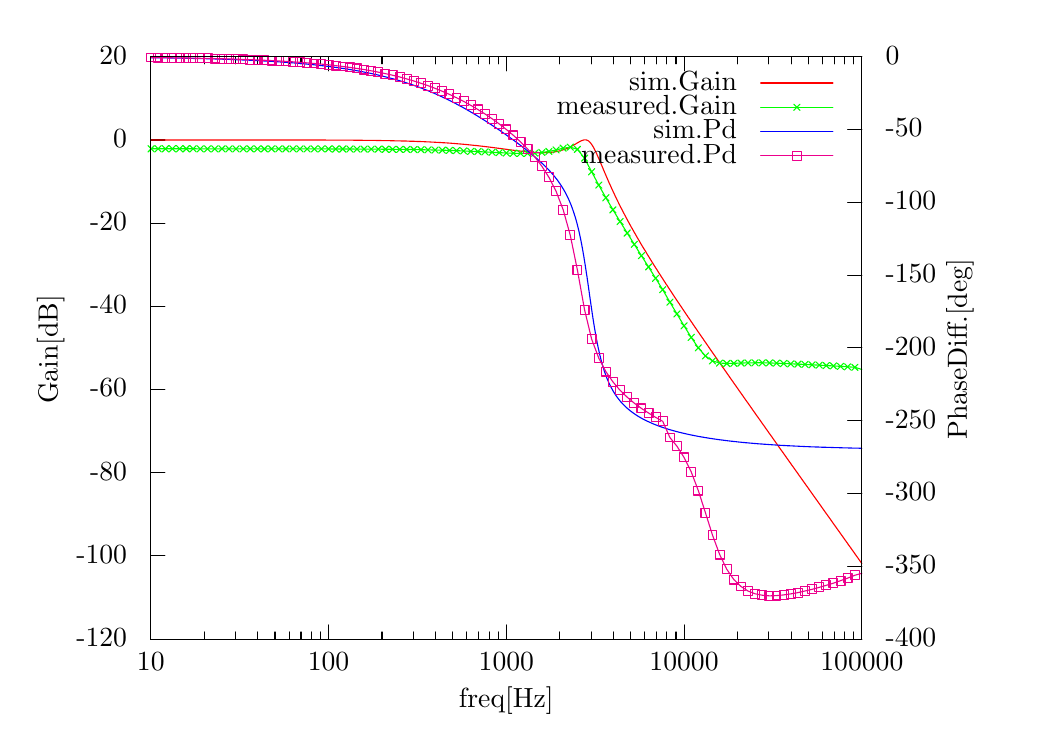
\begin{tikzpicture}[gnuplot]
%% generated with GNUPLOT 4.6p4 (Lua 5.1; terminal rev. 99, script rev. 100)
%% 2016年06月18日 10時13分49秒
\path (0.000,0.000) rectangle (12.500,8.750);
\gpcolor{color=gp lt color border}
\gpsetlinetype{gp lt border}
\gpsetlinewidth{1.00}
\draw[gp path] (1.504,0.985)--(1.684,0.985);
\node[gp node right] at (1.320,0.985) {-120};
\draw[gp path] (1.504,2.042)--(1.684,2.042);
\node[gp node right] at (1.320,2.042) {-100};
\draw[gp path] (1.504,3.098)--(1.684,3.098);
\node[gp node right] at (1.320,3.098) {-80};
\draw[gp path] (1.504,4.155)--(1.684,4.155);
\node[gp node right] at (1.320,4.155) {-60};
\draw[gp path] (1.504,5.211)--(1.684,5.211);
\node[gp node right] at (1.320,5.211) {-40};
\draw[gp path] (1.504,6.268)--(1.684,6.268);
\node[gp node right] at (1.320,6.268) {-20};
\draw[gp path] (1.504,7.324)--(1.684,7.324);
\node[gp node right] at (1.320,7.324) { 0};
\draw[gp path] (1.504,8.381)--(1.684,8.381);
\node[gp node right] at (1.320,8.381) { 20};
\draw[gp path] (1.504,0.985)--(1.504,1.165);
\draw[gp path] (1.504,8.381)--(1.504,8.201);
\node[gp node center] at (1.504,0.677) { 10};
\draw[gp path] (2.184,0.985)--(2.184,1.075);
\draw[gp path] (2.184,8.381)--(2.184,8.291);
\draw[gp path] (2.581,0.985)--(2.581,1.075);
\draw[gp path] (2.581,8.381)--(2.581,8.291);
\draw[gp path] (2.863,0.985)--(2.863,1.075);
\draw[gp path] (2.863,8.381)--(2.863,8.291);
\draw[gp path] (3.082,0.985)--(3.082,1.075);
\draw[gp path] (3.082,8.381)--(3.082,8.291);
\draw[gp path] (3.261,0.985)--(3.261,1.075);
\draw[gp path] (3.261,8.381)--(3.261,8.291);
\draw[gp path] (3.412,0.985)--(3.412,1.075);
\draw[gp path] (3.412,8.381)--(3.412,8.291);
\draw[gp path] (3.543,0.985)--(3.543,1.075);
\draw[gp path] (3.543,8.381)--(3.543,8.291);
\draw[gp path] (3.658,0.985)--(3.658,1.075);
\draw[gp path] (3.658,8.381)--(3.658,8.291);
\draw[gp path] (3.762,0.985)--(3.762,1.165);
\draw[gp path] (3.762,8.381)--(3.762,8.201);
\node[gp node center] at (3.762,0.677) { 100};
\draw[gp path] (4.441,0.985)--(4.441,1.075);
\draw[gp path] (4.441,8.381)--(4.441,8.291);
\draw[gp path] (4.839,0.985)--(4.839,1.075);
\draw[gp path] (4.839,8.381)--(4.839,8.291);
\draw[gp path] (5.121,0.985)--(5.121,1.075);
\draw[gp path] (5.121,8.381)--(5.121,8.291);
\draw[gp path] (5.340,0.985)--(5.340,1.075);
\draw[gp path] (5.340,8.381)--(5.340,8.291);
\draw[gp path] (5.519,0.985)--(5.519,1.075);
\draw[gp path] (5.519,8.381)--(5.519,8.291);
\draw[gp path] (5.670,0.985)--(5.670,1.075);
\draw[gp path] (5.670,8.381)--(5.670,8.291);
\draw[gp path] (5.801,0.985)--(5.801,1.075);
\draw[gp path] (5.801,8.381)--(5.801,8.291);
\draw[gp path] (5.916,0.985)--(5.916,1.075);
\draw[gp path] (5.916,8.381)--(5.916,8.291);
\draw[gp path] (6.020,0.985)--(6.020,1.165);
\draw[gp path] (6.020,8.381)--(6.020,8.201);
\node[gp node center] at (6.020,0.677) { 1000};
\draw[gp path] (6.699,0.985)--(6.699,1.075);
\draw[gp path] (6.699,8.381)--(6.699,8.291);
\draw[gp path] (7.097,0.985)--(7.097,1.075);
\draw[gp path] (7.097,8.381)--(7.097,8.291);
\draw[gp path] (7.379,0.985)--(7.379,1.075);
\draw[gp path] (7.379,8.381)--(7.379,8.291);
\draw[gp path] (7.598,0.985)--(7.598,1.075);
\draw[gp path] (7.598,8.381)--(7.598,8.291);
\draw[gp path] (7.776,0.985)--(7.776,1.075);
\draw[gp path] (7.776,8.381)--(7.776,8.291);
\draw[gp path] (7.928,0.985)--(7.928,1.075);
\draw[gp path] (7.928,8.381)--(7.928,8.291);
\draw[gp path] (8.058,0.985)--(8.058,1.075);
\draw[gp path] (8.058,8.381)--(8.058,8.291);
\draw[gp path] (8.174,0.985)--(8.174,1.075);
\draw[gp path] (8.174,8.381)--(8.174,8.291);
\draw[gp path] (8.277,0.985)--(8.277,1.165);
\draw[gp path] (8.277,8.381)--(8.277,8.201);
\node[gp node center] at (8.277,0.677) { 10000};
\draw[gp path] (8.957,0.985)--(8.957,1.075);
\draw[gp path] (8.957,8.381)--(8.957,8.291);
\draw[gp path] (9.354,0.985)--(9.354,1.075);
\draw[gp path] (9.354,8.381)--(9.354,8.291);
\draw[gp path] (9.637,0.985)--(9.637,1.075);
\draw[gp path] (9.637,8.381)--(9.637,8.291);
\draw[gp path] (9.855,0.985)--(9.855,1.075);
\draw[gp path] (9.855,8.381)--(9.855,8.291);
\draw[gp path] (10.034,0.985)--(10.034,1.075);
\draw[gp path] (10.034,8.381)--(10.034,8.291);
\draw[gp path] (10.185,0.985)--(10.185,1.075);
\draw[gp path] (10.185,8.381)--(10.185,8.291);
\draw[gp path] (10.316,0.985)--(10.316,1.075);
\draw[gp path] (10.316,8.381)--(10.316,8.291);
\draw[gp path] (10.432,0.985)--(10.432,1.075);
\draw[gp path] (10.432,8.381)--(10.432,8.291);
\draw[gp path] (10.535,0.985)--(10.535,1.165);
\draw[gp path] (10.535,8.381)--(10.535,8.201);
\node[gp node center] at (10.535,0.677) { 100000};
\draw[gp path] (10.535,0.985)--(10.355,0.985);
\node[gp node left] at (10.719,0.985) {-400};
\draw[gp path] (10.535,1.910)--(10.355,1.910);
\node[gp node left] at (10.719,1.910) {-350};
\draw[gp path] (10.535,2.834)--(10.355,2.834);
\node[gp node left] at (10.719,2.834) {-300};
\draw[gp path] (10.535,3.758)--(10.355,3.758);
\node[gp node left] at (10.719,3.758) {-250};
\draw[gp path] (10.535,4.683)--(10.355,4.683);
\node[gp node left] at (10.719,4.683) {-200};
\draw[gp path] (10.535,5.608)--(10.355,5.608);
\node[gp node left] at (10.719,5.608) {-150};
\draw[gp path] (10.535,6.532)--(10.355,6.532);
\node[gp node left] at (10.719,6.532) {-100};
\draw[gp path] (10.535,7.456)--(10.355,7.456);
\node[gp node left] at (10.719,7.456) {-50};
\draw[gp path] (10.535,8.381)--(10.355,8.381);
\node[gp node left] at (10.719,8.381) { 0};
\draw[gp path] (1.504,8.381)--(1.504,0.985)--(10.535,0.985)--(10.535,8.381)--cycle;
\node[gp node center,rotate=-270] at (0.246,4.683) {Gain[dB]};
\node[gp node center,rotate=-270] at (11.792,4.683) {PhaseDiff.[deg]};
\node[gp node center] at (6.019,0.215) {freq[Hz]};
\node[gp node right] at (9.067,8.047) {sim.Gain};
\gpcolor{color=gp lt color 0}
\gpsetlinetype{gp lt plot 0}
\draw[gp path] (9.251,8.047)--(10.167,8.047);
\draw[gp path] (1.504,7.324)--(1.509,7.324)--(1.513,7.324)--(1.518,7.324)--(1.522,7.324)%
  --(1.527,7.324)--(1.531,7.324)--(1.536,7.324)--(1.540,7.324)--(1.545,7.324)--(1.549,7.324)%
  --(1.554,7.324)--(1.558,7.324)--(1.563,7.324)--(1.567,7.324)--(1.572,7.324)--(1.576,7.324)%
  --(1.581,7.324)--(1.585,7.324)--(1.590,7.324)--(1.594,7.324)--(1.599,7.324)--(1.603,7.324)%
  --(1.608,7.324)--(1.612,7.324)--(1.617,7.324)--(1.621,7.324)--(1.626,7.324)--(1.630,7.324)%
  --(1.635,7.324)--(1.639,7.324)--(1.644,7.324)--(1.648,7.324)--(1.653,7.324)--(1.658,7.324)%
  --(1.662,7.324)--(1.667,7.324)--(1.671,7.324)--(1.676,7.324)--(1.680,7.324)--(1.685,7.324)%
  --(1.689,7.324)--(1.694,7.324)--(1.698,7.324)--(1.703,7.324)--(1.707,7.324)--(1.712,7.324)%
  --(1.716,7.324)--(1.721,7.324)--(1.725,7.324)--(1.730,7.324)--(1.734,7.324)--(1.739,7.324)%
  --(1.743,7.324)--(1.748,7.324)--(1.752,7.324)--(1.757,7.324)--(1.761,7.324)--(1.766,7.324)%
  --(1.770,7.324)--(1.775,7.324)--(1.779,7.324)--(1.784,7.324)--(1.788,7.324)--(1.793,7.324)%
  --(1.798,7.324)--(1.802,7.324)--(1.807,7.324)--(1.811,7.324)--(1.816,7.324)--(1.820,7.324)%
  --(1.825,7.324)--(1.829,7.324)--(1.834,7.324)--(1.838,7.324)--(1.843,7.324)--(1.847,7.324)%
  --(1.852,7.324)--(1.856,7.324)--(1.861,7.324)--(1.865,7.324)--(1.870,7.324)--(1.874,7.324)%
  --(1.879,7.324)--(1.883,7.324)--(1.888,7.324)--(1.892,7.324)--(1.897,7.324)--(1.901,7.324)%
  --(1.906,7.324)--(1.910,7.324)--(1.915,7.324)--(1.919,7.324)--(1.924,7.324)--(1.928,7.324)%
  --(1.933,7.324)--(1.937,7.324)--(1.942,7.324)--(1.947,7.324)--(1.951,7.324)--(1.956,7.324)%
  --(1.960,7.324)--(1.965,7.324)--(1.969,7.324)--(1.974,7.324)--(1.978,7.324)--(1.983,7.324)%
  --(1.987,7.324)--(1.992,7.324)--(1.996,7.324)--(2.001,7.324)--(2.005,7.324)--(2.010,7.324)%
  --(2.014,7.324)--(2.019,7.324)--(2.023,7.324)--(2.028,7.324)--(2.032,7.324)--(2.037,7.324)%
  --(2.041,7.324)--(2.046,7.324)--(2.050,7.324)--(2.055,7.324)--(2.059,7.324)--(2.064,7.324)%
  --(2.068,7.324)--(2.073,7.324)--(2.077,7.324)--(2.082,7.324)--(2.086,7.324)--(2.091,7.324)%
  --(2.096,7.324)--(2.100,7.324)--(2.105,7.324)--(2.109,7.324)--(2.114,7.324)--(2.118,7.324)%
  --(2.123,7.324)--(2.127,7.324)--(2.132,7.324)--(2.136,7.324)--(2.141,7.324)--(2.145,7.324)%
  --(2.150,7.324)--(2.154,7.324)--(2.159,7.324)--(2.163,7.324)--(2.168,7.324)--(2.172,7.324)%
  --(2.177,7.324)--(2.181,7.324)--(2.186,7.324)--(2.190,7.324)--(2.195,7.324)--(2.199,7.324)%
  --(2.204,7.324)--(2.208,7.324)--(2.213,7.324)--(2.217,7.324)--(2.222,7.324)--(2.226,7.324)%
  --(2.231,7.324)--(2.236,7.324)--(2.240,7.324)--(2.245,7.324)--(2.249,7.324)--(2.254,7.324)%
  --(2.258,7.324)--(2.263,7.324)--(2.267,7.324)--(2.272,7.324)--(2.276,7.324)--(2.281,7.324)%
  --(2.285,7.324)--(2.290,7.324)--(2.294,7.324)--(2.299,7.324)--(2.303,7.324)--(2.308,7.324)%
  --(2.312,7.324)--(2.317,7.324)--(2.321,7.324)--(2.326,7.324)--(2.330,7.324)--(2.335,7.324)%
  --(2.339,7.324)--(2.344,7.324)--(2.348,7.324)--(2.353,7.324)--(2.357,7.324)--(2.362,7.324)%
  --(2.366,7.324)--(2.371,7.324)--(2.375,7.324)--(2.380,7.324)--(2.385,7.324)--(2.389,7.324)%
  --(2.394,7.324)--(2.398,7.324)--(2.403,7.324)--(2.407,7.324)--(2.412,7.324)--(2.416,7.324)%
  --(2.421,7.324)--(2.425,7.324)--(2.430,7.324)--(2.434,7.324)--(2.439,7.324)--(2.443,7.324)%
  --(2.448,7.324)--(2.452,7.324)--(2.457,7.324)--(2.461,7.324)--(2.466,7.324)--(2.470,7.324)%
  --(2.475,7.324)--(2.479,7.324)--(2.484,7.324)--(2.488,7.324)--(2.493,7.324)--(2.497,7.324)%
  --(2.502,7.324)--(2.506,7.324)--(2.511,7.324)--(2.515,7.324)--(2.520,7.324)--(2.525,7.324)%
  --(2.529,7.324)--(2.534,7.324)--(2.538,7.324)--(2.543,7.324)--(2.547,7.324)--(2.552,7.324)%
  --(2.556,7.324)--(2.561,7.324)--(2.565,7.324)--(2.570,7.324)--(2.574,7.324)--(2.579,7.324)%
  --(2.583,7.324)--(2.588,7.324)--(2.592,7.324)--(2.597,7.324)--(2.601,7.324)--(2.606,7.324)%
  --(2.610,7.324)--(2.615,7.324)--(2.619,7.324)--(2.624,7.324)--(2.628,7.324)--(2.633,7.324)%
  --(2.637,7.324)--(2.642,7.324)--(2.646,7.324)--(2.651,7.324)--(2.655,7.324)--(2.660,7.324)%
  --(2.664,7.324)--(2.669,7.324)--(2.674,7.324)--(2.678,7.324)--(2.683,7.324)--(2.687,7.324)%
  --(2.692,7.324)--(2.696,7.324)--(2.701,7.324)--(2.705,7.324)--(2.710,7.324)--(2.714,7.324)%
  --(2.719,7.324)--(2.723,7.324)--(2.728,7.324)--(2.732,7.324)--(2.737,7.324)--(2.741,7.324)%
  --(2.746,7.324)--(2.750,7.324)--(2.755,7.324)--(2.759,7.324)--(2.764,7.324)--(2.768,7.324)%
  --(2.773,7.324)--(2.777,7.324)--(2.782,7.324)--(2.786,7.324)--(2.791,7.324)--(2.795,7.324)%
  --(2.800,7.324)--(2.804,7.324)--(2.809,7.324)--(2.813,7.324)--(2.818,7.324)--(2.823,7.324)%
  --(2.827,7.324)--(2.832,7.324)--(2.836,7.324)--(2.841,7.324)--(2.845,7.324)--(2.850,7.324)%
  --(2.854,7.324)--(2.859,7.324)--(2.863,7.324)--(2.868,7.324)--(2.872,7.324)--(2.877,7.324)%
  --(2.881,7.324)--(2.886,7.324)--(2.890,7.324)--(2.895,7.324)--(2.899,7.324)--(2.904,7.324)%
  --(2.908,7.324)--(2.913,7.324)--(2.917,7.324)--(2.922,7.324)--(2.926,7.324)--(2.931,7.324)%
  --(2.935,7.324)--(2.940,7.324)--(2.944,7.324)--(2.949,7.324)--(2.953,7.324)--(2.958,7.324)%
  --(2.963,7.324)--(2.967,7.324)--(2.972,7.324)--(2.976,7.324)--(2.981,7.324)--(2.985,7.324)%
  --(2.990,7.324)--(2.994,7.324)--(2.999,7.324)--(3.003,7.324)--(3.008,7.324)--(3.012,7.324)%
  --(3.017,7.324)--(3.021,7.324)--(3.026,7.324)--(3.030,7.324)--(3.035,7.324)--(3.039,7.324)%
  --(3.044,7.324)--(3.048,7.324)--(3.053,7.324)--(3.057,7.324)--(3.062,7.324)--(3.066,7.324)%
  --(3.071,7.324)--(3.075,7.324)--(3.080,7.324)--(3.084,7.324)--(3.089,7.324)--(3.093,7.324)%
  --(3.098,7.324)--(3.102,7.324)--(3.107,7.324)--(3.112,7.324)--(3.116,7.324)--(3.121,7.324)%
  --(3.125,7.324)--(3.130,7.324)--(3.134,7.324)--(3.139,7.324)--(3.143,7.324)--(3.148,7.324)%
  --(3.152,7.324)--(3.157,7.324)--(3.161,7.324)--(3.166,7.324)--(3.170,7.324)--(3.175,7.324)%
  --(3.179,7.324)--(3.184,7.324)--(3.188,7.324)--(3.193,7.324)--(3.197,7.324)--(3.202,7.324)%
  --(3.206,7.324)--(3.211,7.324)--(3.215,7.324)--(3.220,7.324)--(3.224,7.324)--(3.229,7.324)%
  --(3.233,7.324)--(3.238,7.324)--(3.242,7.324)--(3.247,7.324)--(3.251,7.324)--(3.256,7.324)%
  --(3.261,7.324)--(3.265,7.324)--(3.270,7.324)--(3.274,7.324)--(3.279,7.324)--(3.283,7.324)%
  --(3.288,7.324)--(3.292,7.324)--(3.297,7.324)--(3.301,7.324)--(3.306,7.324)--(3.310,7.324)%
  --(3.315,7.324)--(3.319,7.324)--(3.324,7.324)--(3.328,7.324)--(3.333,7.324)--(3.337,7.324)%
  --(3.342,7.324)--(3.346,7.324)--(3.351,7.324)--(3.355,7.324)--(3.360,7.324)--(3.364,7.324)%
  --(3.369,7.324)--(3.373,7.323)--(3.378,7.323)--(3.382,7.323)--(3.387,7.323)--(3.391,7.323)%
  --(3.396,7.323)--(3.401,7.323)--(3.405,7.323)--(3.410,7.323)--(3.414,7.323)--(3.419,7.323)%
  --(3.423,7.323)--(3.428,7.323)--(3.432,7.323)--(3.437,7.323)--(3.441,7.323)--(3.446,7.323)%
  --(3.450,7.323)--(3.455,7.323)--(3.459,7.323)--(3.464,7.323)--(3.468,7.323)--(3.473,7.323)%
  --(3.477,7.323)--(3.482,7.323)--(3.486,7.323)--(3.491,7.323)--(3.495,7.323)--(3.500,7.323)%
  --(3.504,7.323)--(3.509,7.323)--(3.513,7.323)--(3.518,7.323)--(3.522,7.323)--(3.527,7.323)%
  --(3.531,7.323)--(3.536,7.323)--(3.540,7.323)--(3.545,7.323)--(3.550,7.323)--(3.554,7.323)%
  --(3.559,7.323)--(3.563,7.323)--(3.568,7.323)--(3.572,7.323)--(3.577,7.323)--(3.581,7.323)%
  --(3.586,7.323)--(3.590,7.323)--(3.595,7.323)--(3.599,7.323)--(3.604,7.323)--(3.608,7.323)%
  --(3.613,7.323)--(3.617,7.323)--(3.622,7.323)--(3.626,7.323)--(3.631,7.323)--(3.635,7.323)%
  --(3.640,7.323)--(3.644,7.323)--(3.649,7.323)--(3.653,7.323)--(3.658,7.323)--(3.662,7.323)%
  --(3.667,7.323)--(3.671,7.323)--(3.676,7.323)--(3.680,7.323)--(3.685,7.323)--(3.690,7.323)%
  --(3.694,7.323)--(3.699,7.323)--(3.703,7.323)--(3.708,7.323)--(3.712,7.323)--(3.717,7.323)%
  --(3.721,7.323)--(3.726,7.323)--(3.730,7.322)--(3.735,7.322)--(3.739,7.322)--(3.744,7.322)%
  --(3.748,7.322)--(3.753,7.322)--(3.757,7.322)--(3.762,7.322)--(3.766,7.322)--(3.771,7.322)%
  --(3.775,7.322)--(3.780,7.322)--(3.784,7.322)--(3.789,7.322)--(3.793,7.322)--(3.798,7.322)%
  --(3.802,7.322)--(3.807,7.322)--(3.811,7.322)--(3.816,7.322)--(3.820,7.322)--(3.825,7.322)%
  --(3.829,7.322)--(3.834,7.322)--(3.839,7.322)--(3.843,7.322)--(3.848,7.322)--(3.852,7.322)%
  --(3.857,7.322)--(3.861,7.322)--(3.866,7.322)--(3.870,7.322)--(3.875,7.322)--(3.879,7.322)%
  --(3.884,7.322)--(3.888,7.322)--(3.893,7.322)--(3.897,7.322)--(3.902,7.322)--(3.906,7.322)%
  --(3.911,7.322)--(3.915,7.322)--(3.920,7.322)--(3.924,7.322)--(3.929,7.322)--(3.933,7.322)%
  --(3.938,7.321)--(3.942,7.321)--(3.947,7.321)--(3.951,7.321)--(3.956,7.321)--(3.960,7.321)%
  --(3.965,7.321)--(3.969,7.321)--(3.974,7.321)--(3.978,7.321)--(3.983,7.321)--(3.988,7.321)%
  --(3.992,7.321)--(3.997,7.321)--(4.001,7.321)--(4.006,7.321)--(4.010,7.321)--(4.015,7.321)%
  --(4.019,7.321)--(4.024,7.321)--(4.028,7.321)--(4.033,7.321)--(4.037,7.321)--(4.042,7.321)%
  --(4.046,7.321)--(4.051,7.321)--(4.055,7.321)--(4.060,7.321)--(4.064,7.321)--(4.069,7.321)%
  --(4.073,7.321)--(4.078,7.321)--(4.082,7.320)--(4.087,7.320)--(4.091,7.320)--(4.096,7.320)%
  --(4.100,7.320)--(4.105,7.320)--(4.109,7.320)--(4.114,7.320)--(4.118,7.320)--(4.123,7.320)%
  --(4.128,7.320)--(4.132,7.320)--(4.137,7.320)--(4.141,7.320)--(4.146,7.320)--(4.150,7.320)%
  --(4.155,7.320)--(4.159,7.320)--(4.164,7.320)--(4.168,7.320)--(4.173,7.320)--(4.177,7.320)%
  --(4.182,7.320)--(4.186,7.320)--(4.191,7.320)--(4.195,7.319)--(4.200,7.319)--(4.204,7.319)%
  --(4.209,7.319)--(4.213,7.319)--(4.218,7.319)--(4.222,7.319)--(4.227,7.319)--(4.231,7.319)%
  --(4.236,7.319)--(4.240,7.319)--(4.245,7.319)--(4.249,7.319)--(4.254,7.319)--(4.258,7.319)%
  --(4.263,7.319)--(4.267,7.319)--(4.272,7.319)--(4.277,7.319)--(4.281,7.319)--(4.286,7.319)%
  --(4.290,7.318)--(4.295,7.318)--(4.299,7.318)--(4.304,7.318)--(4.308,7.318)--(4.313,7.318)%
  --(4.317,7.318)--(4.322,7.318)--(4.326,7.318)--(4.331,7.318)--(4.335,7.318)--(4.340,7.318)%
  --(4.344,7.318)--(4.349,7.318)--(4.353,7.318)--(4.358,7.318)--(4.362,7.318)--(4.367,7.317)%
  --(4.371,7.317)--(4.376,7.317)--(4.380,7.317)--(4.385,7.317)--(4.389,7.317)--(4.394,7.317)%
  --(4.398,7.317)--(4.403,7.317)--(4.407,7.317)--(4.412,7.317)--(4.416,7.317)--(4.421,7.317)%
  --(4.426,7.317)--(4.430,7.317)--(4.435,7.316)--(4.439,7.316)--(4.444,7.316)--(4.448,7.316)%
  --(4.453,7.316)--(4.457,7.316)--(4.462,7.316)--(4.466,7.316)--(4.471,7.316)--(4.475,7.316)%
  --(4.480,7.316)--(4.484,7.316)--(4.489,7.316)--(4.493,7.315)--(4.498,7.315)--(4.502,7.315)%
  --(4.507,7.315)--(4.511,7.315)--(4.516,7.315)--(4.520,7.315)--(4.525,7.315)--(4.529,7.315)%
  --(4.534,7.315)--(4.538,7.315)--(4.543,7.315)--(4.547,7.314)--(4.552,7.314)--(4.556,7.314)%
  --(4.561,7.314)--(4.566,7.314)--(4.570,7.314)--(4.575,7.314)--(4.579,7.314)--(4.584,7.314)%
  --(4.588,7.314)--(4.593,7.314)--(4.597,7.313)--(4.602,7.313)--(4.606,7.313)--(4.611,7.313)%
  --(4.615,7.313)--(4.620,7.313)--(4.624,7.313)--(4.629,7.313)--(4.633,7.313)--(4.638,7.313)%
  --(4.642,7.312)--(4.647,7.312)--(4.651,7.312)--(4.656,7.312)--(4.660,7.312)--(4.665,7.312)%
  --(4.669,7.312)--(4.674,7.312)--(4.678,7.312)--(4.683,7.311)--(4.687,7.311)--(4.692,7.311)%
  --(4.696,7.311)--(4.701,7.311)--(4.705,7.311)--(4.710,7.311)--(4.715,7.311)--(4.719,7.311)%
  --(4.724,7.310)--(4.728,7.310)--(4.733,7.310)--(4.737,7.310)--(4.742,7.310)--(4.746,7.310)%
  --(4.751,7.310)--(4.755,7.310)--(4.760,7.309)--(4.764,7.309)--(4.769,7.309)--(4.773,7.309)%
  --(4.778,7.309)--(4.782,7.309)--(4.787,7.309)--(4.791,7.308)--(4.796,7.308)--(4.800,7.308)%
  --(4.805,7.308)--(4.809,7.308)--(4.814,7.308)--(4.818,7.308)--(4.823,7.307)--(4.827,7.307)%
  --(4.832,7.307)--(4.836,7.307)--(4.841,7.307)--(4.845,7.307)--(4.850,7.307)--(4.855,7.306)%
  --(4.859,7.306)--(4.864,7.306)--(4.868,7.306)--(4.873,7.306)--(4.877,7.306)--(4.882,7.305)%
  --(4.886,7.305)--(4.891,7.305)--(4.895,7.305)--(4.900,7.305)--(4.904,7.305)--(4.909,7.304)%
  --(4.913,7.304)--(4.918,7.304)--(4.922,7.304)--(4.927,7.304)--(4.931,7.304)--(4.936,7.303)%
  --(4.940,7.303)--(4.945,7.303)--(4.949,7.303)--(4.954,7.303)--(4.958,7.302)--(4.963,7.302)%
  --(4.967,7.302)--(4.972,7.302)--(4.976,7.302)--(4.981,7.301)--(4.985,7.301)--(4.990,7.301)%
  --(4.994,7.301)--(4.999,7.301)--(5.004,7.300)--(5.008,7.300)--(5.013,7.300)--(5.017,7.300)%
  --(5.022,7.300)--(5.026,7.299)--(5.031,7.299)--(5.035,7.299)--(5.040,7.299)--(5.044,7.299)%
  --(5.049,7.298)--(5.053,7.298)--(5.058,7.298)--(5.062,7.298)--(5.067,7.297)--(5.071,7.297)%
  --(5.076,7.297)--(5.080,7.297)--(5.085,7.297)--(5.089,7.296)--(5.094,7.296)--(5.098,7.296)%
  --(5.103,7.296)--(5.107,7.295)--(5.112,7.295)--(5.116,7.295)--(5.121,7.295)--(5.125,7.294)%
  --(5.130,7.294)--(5.134,7.294)--(5.139,7.294)--(5.143,7.293)--(5.148,7.293)--(5.153,7.293)%
  --(5.157,7.293)--(5.162,7.292)--(5.166,7.292)--(5.171,7.292)--(5.175,7.292)--(5.180,7.291)%
  --(5.184,7.291)--(5.189,7.291)--(5.193,7.290)--(5.198,7.290)--(5.202,7.290)--(5.207,7.290)%
  --(5.211,7.289)--(5.216,7.289)--(5.220,7.289)--(5.225,7.289)--(5.229,7.288)--(5.234,7.288)%
  --(5.238,7.288)--(5.243,7.287)--(5.247,7.287)--(5.252,7.287)--(5.256,7.286)--(5.261,7.286)%
  --(5.265,7.286)--(5.270,7.286)--(5.274,7.285)--(5.279,7.285)--(5.283,7.285)--(5.288,7.284)%
  --(5.293,7.284)--(5.297,7.284)--(5.302,7.283)--(5.306,7.283)--(5.311,7.283)--(5.315,7.282)%
  --(5.320,7.282)--(5.324,7.282)--(5.329,7.281)--(5.333,7.281)--(5.338,7.281)--(5.342,7.280)%
  --(5.347,7.280)--(5.351,7.280)--(5.356,7.279)--(5.360,7.279)--(5.365,7.279)--(5.369,7.278)%
  --(5.374,7.278)--(5.378,7.277)--(5.383,7.277)--(5.387,7.277)--(5.392,7.276)--(5.396,7.276)%
  --(5.401,7.276)--(5.405,7.275)--(5.410,7.275)--(5.414,7.274)--(5.419,7.274)--(5.423,7.274)%
  --(5.428,7.273)--(5.432,7.273)--(5.437,7.273)--(5.442,7.272)--(5.446,7.272)--(5.451,7.271)%
  --(5.455,7.271)--(5.460,7.271)--(5.464,7.270)--(5.469,7.270)--(5.473,7.269)--(5.478,7.269)%
  --(5.482,7.268)--(5.487,7.268)--(5.491,7.268)--(5.496,7.267)--(5.500,7.267)--(5.505,7.266)%
  --(5.509,7.266)--(5.514,7.266)--(5.518,7.265)--(5.523,7.265)--(5.527,7.264)--(5.532,7.264)%
  --(5.536,7.263)--(5.541,7.263)--(5.545,7.262)--(5.550,7.262)--(5.554,7.262)--(5.559,7.261)%
  --(5.563,7.261)--(5.568,7.260)--(5.572,7.260)--(5.577,7.259)--(5.581,7.259)--(5.586,7.258)%
  --(5.591,7.258)--(5.595,7.257)--(5.600,7.257)--(5.604,7.256)--(5.609,7.256)--(5.613,7.255)%
  --(5.618,7.255)--(5.622,7.254)--(5.627,7.254)--(5.631,7.254)--(5.636,7.253)--(5.640,7.253)%
  --(5.645,7.252)--(5.649,7.252)--(5.654,7.251)--(5.658,7.251)--(5.663,7.250)--(5.667,7.250)%
  --(5.672,7.249)--(5.676,7.248)--(5.681,7.248)--(5.685,7.247)--(5.690,7.247)--(5.694,7.246)%
  --(5.699,7.246)--(5.703,7.245)--(5.708,7.245)--(5.712,7.244)--(5.717,7.244)--(5.721,7.243)%
  --(5.726,7.243)--(5.731,7.242)--(5.735,7.242)--(5.740,7.241)--(5.744,7.241)--(5.749,7.240)%
  --(5.753,7.239)--(5.758,7.239)--(5.762,7.238)--(5.767,7.238)--(5.771,7.237)--(5.776,7.237)%
  --(5.780,7.236)--(5.785,7.236)--(5.789,7.235)--(5.794,7.234)--(5.798,7.234)--(5.803,7.233)%
  --(5.807,7.233)--(5.812,7.232)--(5.816,7.232)--(5.821,7.231)--(5.825,7.231)--(5.830,7.230)%
  --(5.834,7.229)--(5.839,7.229)--(5.843,7.228)--(5.848,7.228)--(5.852,7.227)--(5.857,7.226)%
  --(5.861,7.226)--(5.866,7.225)--(5.870,7.225)--(5.875,7.224)--(5.880,7.224)--(5.884,7.223)%
  --(5.889,7.222)--(5.893,7.222)--(5.898,7.221)--(5.902,7.221)--(5.907,7.220)--(5.911,7.219)%
  --(5.916,7.219)--(5.920,7.218)--(5.925,7.218)--(5.929,7.217)--(5.934,7.216)--(5.938,7.216)%
  --(5.943,7.215)--(5.947,7.215)--(5.952,7.214)--(5.956,7.213)--(5.961,7.213)--(5.965,7.212)%
  --(5.970,7.212)--(5.974,7.211)--(5.979,7.210)--(5.983,7.210)--(5.988,7.209)--(5.992,7.209)%
  --(5.997,7.208)--(6.001,7.207)--(6.006,7.207)--(6.010,7.206)--(6.015,7.206)--(6.020,7.205)%
  --(6.024,7.204)--(6.029,7.204)--(6.033,7.203)--(6.038,7.203)--(6.042,7.202)--(6.047,7.201)%
  --(6.051,7.201)--(6.056,7.200)--(6.060,7.200)--(6.065,7.199)--(6.069,7.198)--(6.074,7.198)%
  --(6.078,7.197)--(6.083,7.197)--(6.087,7.196)--(6.092,7.195)--(6.096,7.195)--(6.101,7.194)%
  --(6.105,7.194)--(6.110,7.193)--(6.114,7.193)--(6.119,7.192)--(6.123,7.191)--(6.128,7.191)%
  --(6.132,7.190)--(6.137,7.190)--(6.141,7.189)--(6.146,7.189)--(6.150,7.188)--(6.155,7.187)%
  --(6.159,7.187)--(6.164,7.186)--(6.169,7.186)--(6.173,7.185)--(6.178,7.185)--(6.182,7.184)%
  --(6.187,7.184)--(6.191,7.183)--(6.196,7.183)--(6.200,7.182)--(6.205,7.181)--(6.209,7.181)%
  --(6.214,7.180)--(6.218,7.180)--(6.223,7.179)--(6.227,7.179)--(6.232,7.178)--(6.236,7.178)%
  --(6.241,7.177)--(6.245,7.177)--(6.250,7.176)--(6.254,7.176)--(6.259,7.176)--(6.263,7.175)%
  --(6.268,7.175)--(6.272,7.174)--(6.277,7.174)--(6.281,7.173)--(6.286,7.173)--(6.290,7.172)%
  --(6.295,7.172)--(6.299,7.172)--(6.304,7.171)--(6.308,7.171)--(6.313,7.170)--(6.318,7.170)%
  --(6.322,7.170)--(6.327,7.169)--(6.331,7.169)--(6.336,7.169)--(6.340,7.168)--(6.345,7.168)%
  --(6.349,7.167)--(6.354,7.167)--(6.358,7.167)--(6.363,7.167)--(6.367,7.166)--(6.372,7.166)%
  --(6.376,7.166)--(6.381,7.165)--(6.385,7.165)--(6.390,7.165)--(6.394,7.165)--(6.399,7.164)%
  --(6.403,7.164)--(6.408,7.164)--(6.412,7.164)--(6.417,7.164)--(6.421,7.163)--(6.426,7.163)%
  --(6.430,7.163)--(6.435,7.163)--(6.439,7.163)--(6.444,7.163)--(6.448,7.163)--(6.453,7.163)%
  --(6.458,7.162)--(6.462,7.162)--(6.467,7.162)--(6.471,7.162)--(6.476,7.162)--(6.480,7.162)%
  --(6.485,7.162)--(6.489,7.162)--(6.494,7.162)--(6.498,7.162)--(6.503,7.162)--(6.507,7.163)%
  --(6.512,7.163)--(6.516,7.163)--(6.521,7.163)--(6.525,7.163)--(6.530,7.163)--(6.534,7.163)%
  --(6.539,7.164)--(6.543,7.164)--(6.548,7.164)--(6.552,7.164)--(6.557,7.165)--(6.561,7.165)%
  --(6.566,7.165)--(6.570,7.166)--(6.575,7.166)--(6.579,7.166)--(6.584,7.167)--(6.588,7.167)%
  --(6.593,7.168)--(6.597,7.168)--(6.602,7.169)--(6.607,7.169)--(6.611,7.170)--(6.616,7.170)%
  --(6.620,7.171)--(6.625,7.171)--(6.629,7.172)--(6.634,7.173)--(6.638,7.174)--(6.643,7.174)%
  --(6.647,7.175)--(6.652,7.176)--(6.656,7.177)--(6.661,7.177)--(6.665,7.178)--(6.670,7.179)%
  --(6.674,7.180)--(6.679,7.181)--(6.683,7.182)--(6.688,7.183)--(6.692,7.184)--(6.697,7.185)%
  --(6.701,7.186)--(6.706,7.188)--(6.710,7.189)--(6.715,7.190)--(6.719,7.191)--(6.724,7.193)%
  --(6.728,7.194)--(6.733,7.195)--(6.737,7.197)--(6.742,7.198)--(6.746,7.200)--(6.751,7.201)%
  --(6.756,7.203)--(6.760,7.204)--(6.765,7.206)--(6.769,7.208)--(6.774,7.209)--(6.778,7.211)%
  --(6.783,7.213)--(6.787,7.215)--(6.792,7.217)--(6.796,7.218)--(6.801,7.220)--(6.805,7.222)%
  --(6.810,7.225)--(6.814,7.227)--(6.819,7.229)--(6.823,7.231)--(6.828,7.233)--(6.832,7.235)%
  --(6.837,7.238)--(6.841,7.240)--(6.846,7.242)--(6.850,7.245)--(6.855,7.247)--(6.859,7.250)%
  --(6.864,7.252)--(6.868,7.255)--(6.873,7.257)--(6.877,7.260)--(6.882,7.262)--(6.886,7.265)%
  --(6.891,7.268)--(6.896,7.270)--(6.900,7.273)--(6.905,7.276)--(6.909,7.278)--(6.914,7.281)%
  --(6.918,7.284)--(6.923,7.287)--(6.927,7.289)--(6.932,7.292)--(6.936,7.294)--(6.941,7.297)%
  --(6.945,7.300)--(6.950,7.302)--(6.954,7.305)--(6.959,7.307)--(6.963,7.309)--(6.968,7.311)%
  --(6.972,7.313)--(6.977,7.315)--(6.981,7.317)--(6.986,7.319)--(6.990,7.320)--(6.995,7.322)%
  --(6.999,7.323)--(7.004,7.324)--(7.008,7.325)--(7.013,7.325)--(7.017,7.325)--(7.022,7.325)%
  --(7.026,7.325)--(7.031,7.325)--(7.035,7.324)--(7.040,7.323)--(7.045,7.321)--(7.049,7.319)%
  --(7.054,7.317)--(7.058,7.314)--(7.063,7.311)--(7.067,7.308)--(7.072,7.304)--(7.076,7.300)%
  --(7.081,7.296)--(7.085,7.291)--(7.090,7.286)--(7.094,7.280)--(7.099,7.274)--(7.103,7.268)%
  --(7.108,7.261)--(7.112,7.254)--(7.117,7.247)--(7.121,7.239)--(7.126,7.231)--(7.130,7.223)%
  --(7.135,7.215)--(7.139,7.206)--(7.144,7.197)--(7.148,7.188)--(7.153,7.179)--(7.157,7.169)%
  --(7.162,7.160)--(7.166,7.150)--(7.171,7.140)--(7.175,7.130)--(7.180,7.120)--(7.184,7.110)%
  --(7.189,7.099)--(7.194,7.089)--(7.198,7.078)--(7.203,7.068)--(7.207,7.057)--(7.212,7.046)%
  --(7.216,7.036)--(7.221,7.025)--(7.225,7.014)--(7.230,7.004)--(7.234,6.993)--(7.239,6.982)%
  --(7.243,6.971)--(7.248,6.961)--(7.252,6.950)--(7.257,6.939)--(7.261,6.929)--(7.266,6.918)%
  --(7.270,6.907)--(7.275,6.897)--(7.279,6.886)--(7.284,6.876)--(7.288,6.865)--(7.293,6.855)%
  --(7.297,6.844)--(7.302,6.834)--(7.306,6.823)--(7.311,6.813)--(7.315,6.803)--(7.320,6.792)%
  --(7.324,6.782)--(7.329,6.772)--(7.334,6.762)--(7.338,6.752)--(7.343,6.742)--(7.347,6.732)%
  --(7.352,6.722)--(7.356,6.712)--(7.361,6.702)--(7.365,6.692)--(7.370,6.682)--(7.374,6.673)%
  --(7.379,6.663)--(7.383,6.653)--(7.388,6.644)--(7.392,6.634)--(7.397,6.625)--(7.401,6.615)%
  --(7.406,6.606)--(7.410,6.596)--(7.415,6.587)--(7.419,6.578)--(7.424,6.568)--(7.428,6.559)%
  --(7.433,6.550)--(7.437,6.541)--(7.442,6.531)--(7.446,6.522)--(7.451,6.513)--(7.455,6.504)%
  --(7.460,6.495)--(7.464,6.486)--(7.469,6.477)--(7.473,6.468)--(7.478,6.459)--(7.483,6.451)%
  --(7.487,6.442)--(7.492,6.433)--(7.496,6.424)--(7.501,6.415)--(7.505,6.407)--(7.510,6.398)%
  --(7.514,6.389)--(7.519,6.381)--(7.523,6.372)--(7.528,6.364)--(7.532,6.355)--(7.537,6.347)%
  --(7.541,6.338)--(7.546,6.330)--(7.550,6.321)--(7.555,6.313)--(7.559,6.305)--(7.564,6.296)%
  --(7.568,6.288)--(7.573,6.280)--(7.577,6.272)--(7.582,6.263)--(7.586,6.255)--(7.591,6.247)%
  --(7.595,6.239)--(7.600,6.231)--(7.604,6.222)--(7.609,6.214)--(7.613,6.206)--(7.618,6.198)%
  --(7.623,6.190)--(7.627,6.182)--(7.632,6.174)--(7.636,6.166)--(7.641,6.158)--(7.645,6.150)%
  --(7.650,6.142)--(7.654,6.134)--(7.659,6.127)--(7.663,6.119)--(7.668,6.111)--(7.672,6.103)%
  --(7.677,6.095)--(7.681,6.087)--(7.686,6.080)--(7.690,6.072)--(7.695,6.064)--(7.699,6.056)%
  --(7.704,6.049)--(7.708,6.041)--(7.713,6.033)--(7.717,6.026)--(7.722,6.018)--(7.726,6.010)%
  --(7.731,6.003)--(7.735,5.995)--(7.740,5.988)--(7.744,5.980)--(7.749,5.972)--(7.753,5.965)%
  --(7.758,5.957)--(7.762,5.950)--(7.767,5.942)--(7.772,5.935)--(7.776,5.927)--(7.781,5.920)%
  --(7.785,5.912)--(7.790,5.905)--(7.794,5.898)--(7.799,5.890)--(7.803,5.883)--(7.808,5.875)%
  --(7.812,5.868)--(7.817,5.861)--(7.821,5.853)--(7.826,5.846)--(7.830,5.839)--(7.835,5.831)%
  --(7.839,5.824)--(7.844,5.817)--(7.848,5.809)--(7.853,5.802)--(7.857,5.795)--(7.862,5.788)%
  --(7.866,5.780)--(7.871,5.773)--(7.875,5.766)--(7.880,5.759)--(7.884,5.751)--(7.889,5.744)%
  --(7.893,5.737)--(7.898,5.730)--(7.902,5.723)--(7.907,5.716)--(7.911,5.708)--(7.916,5.701)%
  --(7.921,5.694)--(7.925,5.687)--(7.930,5.680)--(7.934,5.673)--(7.939,5.666)--(7.943,5.659)%
  --(7.948,5.651)--(7.952,5.644)--(7.957,5.637)--(7.961,5.630)--(7.966,5.623)--(7.970,5.616)%
  --(7.975,5.609)--(7.979,5.602)--(7.984,5.595)--(7.988,5.588)--(7.993,5.581)--(7.997,5.574)%
  --(8.002,5.567)--(8.006,5.560)--(8.011,5.553)--(8.015,5.546)--(8.020,5.539)--(8.024,5.532)%
  --(8.029,5.525)--(8.033,5.518)--(8.038,5.511)--(8.042,5.504)--(8.047,5.497)--(8.051,5.490)%
  --(8.056,5.484)--(8.061,5.477)--(8.065,5.470)--(8.070,5.463)--(8.074,5.456)--(8.079,5.449)%
  --(8.083,5.442)--(8.088,5.435)--(8.092,5.428)--(8.097,5.421)--(8.101,5.415)--(8.106,5.408)%
  --(8.110,5.401)--(8.115,5.394)--(8.119,5.387)--(8.124,5.380)--(8.128,5.374)--(8.133,5.367)%
  --(8.137,5.360)--(8.142,5.353)--(8.146,5.346)--(8.151,5.339)--(8.155,5.333)--(8.160,5.326)%
  --(8.164,5.319)--(8.169,5.312)--(8.173,5.306)--(8.178,5.299)--(8.182,5.292)--(8.187,5.285)%
  --(8.191,5.278)--(8.196,5.272)--(8.200,5.265)--(8.205,5.258)--(8.210,5.251)--(8.214,5.245)%
  --(8.219,5.238)--(8.223,5.231)--(8.228,5.224)--(8.232,5.218)--(8.237,5.211)--(8.241,5.204)%
  --(8.246,5.198)--(8.250,5.191)--(8.255,5.184)--(8.259,5.177)--(8.264,5.171)--(8.268,5.164)%
  --(8.273,5.157)--(8.277,5.151)--(8.282,5.144)--(8.286,5.137)--(8.291,5.131)--(8.295,5.124)%
  --(8.300,5.117)--(8.304,5.111)--(8.309,5.104)--(8.313,5.097)--(8.318,5.091)--(8.322,5.084)%
  --(8.327,5.077)--(8.331,5.071)--(8.336,5.064)--(8.340,5.057)--(8.345,5.051)--(8.349,5.044)%
  --(8.354,5.037)--(8.359,5.031)--(8.363,5.024)--(8.368,5.017)--(8.372,5.011)--(8.377,5.004)%
  --(8.381,4.998)--(8.386,4.991)--(8.390,4.984)--(8.395,4.978)--(8.399,4.971)--(8.404,4.965)%
  --(8.408,4.958)--(8.413,4.951)--(8.417,4.945)--(8.422,4.938)--(8.426,4.932)--(8.431,4.925)%
  --(8.435,4.918)--(8.440,4.912)--(8.444,4.905)--(8.449,4.899)--(8.453,4.892)--(8.458,4.885)%
  --(8.462,4.879)--(8.467,4.872)--(8.471,4.866)--(8.476,4.859)--(8.480,4.853)--(8.485,4.846)%
  --(8.489,4.839)--(8.494,4.833)--(8.499,4.826)--(8.503,4.820)--(8.508,4.813)--(8.512,4.807)%
  --(8.517,4.800)--(8.521,4.794)--(8.526,4.787)--(8.530,4.780)--(8.535,4.774)--(8.539,4.767)%
  --(8.544,4.761)--(8.548,4.754)--(8.553,4.748)--(8.557,4.741)--(8.562,4.735)--(8.566,4.728)%
  --(8.571,4.722)--(8.575,4.715)--(8.580,4.709)--(8.584,4.702)--(8.589,4.696)--(8.593,4.689)%
  --(8.598,4.683)--(8.602,4.676)--(8.607,4.670)--(8.611,4.663)--(8.616,4.656)--(8.620,4.650)%
  --(8.625,4.643)--(8.629,4.637)--(8.634,4.630)--(8.638,4.624)--(8.643,4.617)--(8.648,4.611)%
  --(8.652,4.604)--(8.657,4.598)--(8.661,4.591)--(8.666,4.585)--(8.670,4.578)--(8.675,4.572)%
  --(8.679,4.566)--(8.684,4.559)--(8.688,4.553)--(8.693,4.546)--(8.697,4.540)--(8.702,4.533)%
  --(8.706,4.527)--(8.711,4.520)--(8.715,4.514)--(8.720,4.507)--(8.724,4.501)--(8.729,4.494)%
  --(8.733,4.488)--(8.738,4.481)--(8.742,4.475)--(8.747,4.468)--(8.751,4.462)--(8.756,4.455)%
  --(8.760,4.449)--(8.765,4.442)--(8.769,4.436)--(8.774,4.430)--(8.778,4.423)--(8.783,4.417)%
  --(8.788,4.410)--(8.792,4.404)--(8.797,4.397)--(8.801,4.391)--(8.806,4.384)--(8.810,4.378)%
  --(8.815,4.371)--(8.819,4.365)--(8.824,4.359)--(8.828,4.352)--(8.833,4.346)--(8.837,4.339)%
  --(8.842,4.333)--(8.846,4.326)--(8.851,4.320)--(8.855,4.313)--(8.860,4.307)--(8.864,4.301)%
  --(8.869,4.294)--(8.873,4.288)--(8.878,4.281)--(8.882,4.275)--(8.887,4.268)--(8.891,4.262)%
  --(8.896,4.256)--(8.900,4.249)--(8.905,4.243)--(8.909,4.236)--(8.914,4.230)--(8.918,4.223)%
  --(8.923,4.217)--(8.927,4.210)--(8.932,4.204)--(8.937,4.198)--(8.941,4.191)--(8.946,4.185)%
  --(8.950,4.178)--(8.955,4.172)--(8.959,4.166)--(8.964,4.159)--(8.968,4.153)--(8.973,4.146)%
  --(8.977,4.140)--(8.982,4.133)--(8.986,4.127)--(8.991,4.121)--(8.995,4.114)--(9.000,4.108)%
  --(9.004,4.101)--(9.009,4.095)--(9.013,4.089)--(9.018,4.082)--(9.022,4.076)--(9.027,4.069)%
  --(9.031,4.063)--(9.036,4.056)--(9.040,4.050)--(9.045,4.044)--(9.049,4.037)--(9.054,4.031)%
  --(9.058,4.024)--(9.063,4.018)--(9.067,4.012)--(9.072,4.005)--(9.076,3.999)--(9.081,3.992)%
  --(9.086,3.986)--(9.090,3.980)--(9.095,3.973)--(9.099,3.967)--(9.104,3.960)--(9.108,3.954)%
  --(9.113,3.948)--(9.117,3.941)--(9.122,3.935)--(9.126,3.928)--(9.131,3.922)--(9.135,3.916)%
  --(9.140,3.909)--(9.144,3.903)--(9.149,3.896)--(9.153,3.890)--(9.158,3.884)--(9.162,3.877)%
  --(9.167,3.871)--(9.171,3.864)--(9.176,3.858)--(9.180,3.852)--(9.185,3.845)--(9.189,3.839)%
  --(9.194,3.832)--(9.198,3.826)--(9.203,3.820)--(9.207,3.813)--(9.212,3.807)--(9.216,3.801)%
  --(9.221,3.794)--(9.226,3.788)--(9.230,3.781)--(9.235,3.775)--(9.239,3.769)--(9.244,3.762)%
  --(9.248,3.756)--(9.253,3.749)--(9.257,3.743)--(9.262,3.737)--(9.266,3.730)--(9.271,3.724)%
  --(9.275,3.718)--(9.280,3.711)--(9.284,3.705)--(9.289,3.698)--(9.293,3.692)--(9.298,3.686)%
  --(9.302,3.679)--(9.307,3.673)--(9.311,3.666)--(9.316,3.660)--(9.320,3.654)--(9.325,3.647)%
  --(9.329,3.641)--(9.334,3.635)--(9.338,3.628)--(9.343,3.622)--(9.347,3.615)--(9.352,3.609)%
  --(9.356,3.603)--(9.361,3.596)--(9.365,3.590)--(9.370,3.584)--(9.375,3.577)--(9.379,3.571)%
  --(9.384,3.564)--(9.388,3.558)--(9.393,3.552)--(9.397,3.545)--(9.402,3.539)--(9.406,3.533)%
  --(9.411,3.526)--(9.415,3.520)--(9.420,3.513)--(9.424,3.507)--(9.429,3.501)--(9.433,3.494)%
  --(9.438,3.488)--(9.442,3.482)--(9.447,3.475)--(9.451,3.469)--(9.456,3.463)--(9.460,3.456)%
  --(9.465,3.450)--(9.469,3.443)--(9.474,3.437)--(9.478,3.431)--(9.483,3.424)--(9.487,3.418)%
  --(9.492,3.412)--(9.496,3.405)--(9.501,3.399)--(9.505,3.392)--(9.510,3.386)--(9.514,3.380)%
  --(9.519,3.373)--(9.524,3.367)--(9.528,3.361)--(9.533,3.354)--(9.537,3.348)--(9.542,3.342)%
  --(9.546,3.335)--(9.551,3.329)--(9.555,3.322)--(9.560,3.316)--(9.564,3.310)--(9.569,3.303)%
  --(9.573,3.297)--(9.578,3.291)--(9.582,3.284)--(9.587,3.278)--(9.591,3.272)--(9.596,3.265)%
  --(9.600,3.259)--(9.605,3.252)--(9.609,3.246)--(9.614,3.240)--(9.618,3.233)--(9.623,3.227)%
  --(9.627,3.221)--(9.632,3.214)--(9.636,3.208)--(9.641,3.202)--(9.645,3.195)--(9.650,3.189)%
  --(9.654,3.183)--(9.659,3.176)--(9.664,3.170)--(9.668,3.163)--(9.673,3.157)--(9.677,3.151)%
  --(9.682,3.144)--(9.686,3.138)--(9.691,3.132)--(9.695,3.125)--(9.700,3.119)--(9.704,3.113)%
  --(9.709,3.106)--(9.713,3.100)--(9.718,3.094)--(9.722,3.087)--(9.727,3.081)--(9.731,3.074)%
  --(9.736,3.068)--(9.740,3.062)--(9.745,3.055)--(9.749,3.049)--(9.754,3.043)--(9.758,3.036)%
  --(9.763,3.030)--(9.767,3.024)--(9.772,3.017)--(9.776,3.011)--(9.781,3.005)--(9.785,2.998)%
  --(9.790,2.992)--(9.794,2.985)--(9.799,2.979)--(9.803,2.973)--(9.808,2.966)--(9.813,2.960)%
  --(9.817,2.954)--(9.822,2.947)--(9.826,2.941)--(9.831,2.935)--(9.835,2.928)--(9.840,2.922)%
  --(9.844,2.916)--(9.849,2.909)--(9.853,2.903)--(9.858,2.897)--(9.862,2.890)--(9.867,2.884)%
  --(9.871,2.877)--(9.876,2.871)--(9.880,2.865)--(9.885,2.858)--(9.889,2.852)--(9.894,2.846)%
  --(9.898,2.839)--(9.903,2.833)--(9.907,2.827)--(9.912,2.820)--(9.916,2.814)--(9.921,2.808)%
  --(9.925,2.801)--(9.930,2.795)--(9.934,2.789)--(9.939,2.782)--(9.943,2.776)--(9.948,2.769)%
  --(9.953,2.763)--(9.957,2.757)--(9.962,2.750)--(9.966,2.744)--(9.971,2.738)--(9.975,2.731)%
  --(9.980,2.725)--(9.984,2.719)--(9.989,2.712)--(9.993,2.706)--(9.998,2.700)--(10.002,2.693)%
  --(10.007,2.687)--(10.011,2.681)--(10.016,2.674)--(10.020,2.668)--(10.025,2.662)--(10.029,2.655)%
  --(10.034,2.649)--(10.038,2.643)--(10.043,2.636)--(10.047,2.630)--(10.052,2.623)--(10.056,2.617)%
  --(10.061,2.611)--(10.065,2.604)--(10.070,2.598)--(10.074,2.592)--(10.079,2.585)--(10.083,2.579)%
  --(10.088,2.573)--(10.092,2.566)--(10.097,2.560)--(10.102,2.554)--(10.106,2.547)--(10.111,2.541)%
  --(10.115,2.535)--(10.120,2.528)--(10.124,2.522)--(10.129,2.516)--(10.133,2.509)--(10.138,2.503)%
  --(10.142,2.497)--(10.147,2.490)--(10.151,2.484)--(10.156,2.477)--(10.160,2.471)--(10.165,2.465)%
  --(10.169,2.458)--(10.174,2.452)--(10.178,2.446)--(10.183,2.439)--(10.187,2.433)--(10.192,2.427)%
  --(10.196,2.420)--(10.201,2.414)--(10.205,2.408)--(10.210,2.401)--(10.214,2.395)--(10.219,2.389)%
  --(10.223,2.382)--(10.228,2.376)--(10.232,2.370)--(10.237,2.363)--(10.241,2.357)--(10.246,2.351)%
  --(10.251,2.344)--(10.255,2.338)--(10.260,2.332)--(10.264,2.325)--(10.269,2.319)--(10.273,2.312)%
  --(10.278,2.306)--(10.282,2.300)--(10.287,2.293)--(10.291,2.287)--(10.296,2.281)--(10.300,2.274)%
  --(10.305,2.268)--(10.309,2.262)--(10.314,2.255)--(10.318,2.249)--(10.323,2.243)--(10.327,2.236)%
  --(10.332,2.230)--(10.336,2.224)--(10.341,2.217)--(10.345,2.211)--(10.350,2.205)--(10.354,2.198)%
  --(10.359,2.192)--(10.363,2.186)--(10.368,2.179)--(10.372,2.173)--(10.377,2.167)--(10.381,2.160)%
  --(10.386,2.154)--(10.391,2.148)--(10.395,2.141)--(10.400,2.135)--(10.404,2.129)--(10.409,2.122)%
  --(10.413,2.116)--(10.418,2.109)--(10.422,2.103)--(10.427,2.097)--(10.431,2.090)--(10.436,2.084)%
  --(10.440,2.078)--(10.445,2.071)--(10.449,2.065)--(10.454,2.059)--(10.458,2.052)--(10.463,2.046)%
  --(10.467,2.040)--(10.472,2.033)--(10.476,2.027)--(10.481,2.021)--(10.485,2.014)--(10.490,2.008)%
  --(10.494,2.002)--(10.499,1.995)--(10.503,1.989)--(10.508,1.983)--(10.512,1.976)--(10.517,1.970)%
  --(10.521,1.964)--(10.526,1.957)--(10.530,1.951)--(10.535,1.945);
\gpcolor{color=gp lt color border}
\node[gp node right] at (9.067,7.739) {measured.Gain};
\gpcolor{color=gp lt color 1}
\gpsetlinetype{gp lt plot 1}
\draw[gp path] (9.251,7.739)--(10.167,7.739);
\draw[gp path] (1.510,7.212)--(1.597,7.212)--(1.691,7.212)--(1.778,7.212)--(1.870,7.212)%
  --(1.955,7.212)--(2.043,7.212)--(2.133,7.211)--(2.225,7.211)--(2.317,7.211)--(2.408,7.211)%
  --(2.498,7.211)--(2.587,7.211)--(2.679,7.211)--(2.769,7.211)--(2.860,7.211)--(2.947,7.211)%
  --(3.039,7.211)--(3.130,7.211)--(3.220,7.211)--(3.311,7.211)--(3.399,7.210)--(3.490,7.210)%
  --(3.582,7.210)--(3.672,7.210)--(3.762,7.210)--(3.853,7.209)--(3.942,7.209)--(4.033,7.209)%
  --(4.123,7.208)--(4.213,7.208)--(4.304,7.207)--(4.394,7.207)--(4.485,7.206)--(4.575,7.205)%
  --(4.665,7.204)--(4.755,7.203)--(4.845,7.202)--(4.936,7.200)--(5.026,7.198)--(5.116,7.196)%
  --(5.207,7.194)--(5.297,7.191)--(5.387,7.188)--(5.478,7.184)--(5.568,7.180)--(5.658,7.176)%
  --(5.749,7.172)--(5.839,7.167)--(5.929,7.163)--(6.020,7.158)--(6.110,7.155)--(6.200,7.153)%
  --(6.290,7.154)--(6.381,7.157)--(6.471,7.165)--(6.561,7.178)--(6.652,7.197)--(6.742,7.219)%
  --(6.832,7.232)--(6.923,7.205)--(7.013,7.092)--(7.103,6.920)--(7.194,6.750)--(7.284,6.590)%
  --(7.374,6.437)--(7.464,6.288)--(7.555,6.142)--(7.645,5.998)--(7.735,5.854)--(7.826,5.711)%
  --(7.916,5.567)--(8.006,5.422)--(8.097,5.264)--(8.187,5.114)--(8.277,4.963)--(8.368,4.816)%
  --(8.458,4.684)--(8.548,4.581)--(8.638,4.518)--(8.729,4.491)--(8.819,4.485)--(8.909,4.487)%
  --(9.000,4.491)--(9.090,4.493)--(9.180,4.494)--(9.271,4.494)--(9.361,4.492)--(9.451,4.489)%
  --(9.542,4.485)--(9.632,4.481)--(9.722,4.477)--(9.813,4.473)--(9.903,4.468)--(9.993,4.464)%
  --(10.083,4.459)--(10.174,4.454)--(10.264,4.449)--(10.354,4.443)--(10.445,4.437)--(10.535,4.409);
\gpsetpointsize{4.00}
\gppoint{gp mark 2}{(1.510,7.212)}
\gppoint{gp mark 2}{(1.597,7.212)}
\gppoint{gp mark 2}{(1.691,7.212)}
\gppoint{gp mark 2}{(1.778,7.212)}
\gppoint{gp mark 2}{(1.870,7.212)}
\gppoint{gp mark 2}{(1.955,7.212)}
\gppoint{gp mark 2}{(2.043,7.212)}
\gppoint{gp mark 2}{(2.133,7.211)}
\gppoint{gp mark 2}{(2.225,7.211)}
\gppoint{gp mark 2}{(2.317,7.211)}
\gppoint{gp mark 2}{(2.408,7.211)}
\gppoint{gp mark 2}{(2.498,7.211)}
\gppoint{gp mark 2}{(2.587,7.211)}
\gppoint{gp mark 2}{(2.679,7.211)}
\gppoint{gp mark 2}{(2.769,7.211)}
\gppoint{gp mark 2}{(2.860,7.211)}
\gppoint{gp mark 2}{(2.947,7.211)}
\gppoint{gp mark 2}{(3.039,7.211)}
\gppoint{gp mark 2}{(3.130,7.211)}
\gppoint{gp mark 2}{(3.220,7.211)}
\gppoint{gp mark 2}{(3.311,7.211)}
\gppoint{gp mark 2}{(3.399,7.210)}
\gppoint{gp mark 2}{(3.490,7.210)}
\gppoint{gp mark 2}{(3.582,7.210)}
\gppoint{gp mark 2}{(3.672,7.210)}
\gppoint{gp mark 2}{(3.762,7.210)}
\gppoint{gp mark 2}{(3.853,7.209)}
\gppoint{gp mark 2}{(3.942,7.209)}
\gppoint{gp mark 2}{(4.033,7.209)}
\gppoint{gp mark 2}{(4.123,7.208)}
\gppoint{gp mark 2}{(4.213,7.208)}
\gppoint{gp mark 2}{(4.304,7.207)}
\gppoint{gp mark 2}{(4.394,7.207)}
\gppoint{gp mark 2}{(4.485,7.206)}
\gppoint{gp mark 2}{(4.575,7.205)}
\gppoint{gp mark 2}{(4.665,7.204)}
\gppoint{gp mark 2}{(4.755,7.203)}
\gppoint{gp mark 2}{(4.845,7.202)}
\gppoint{gp mark 2}{(4.936,7.200)}
\gppoint{gp mark 2}{(5.026,7.198)}
\gppoint{gp mark 2}{(5.116,7.196)}
\gppoint{gp mark 2}{(5.207,7.194)}
\gppoint{gp mark 2}{(5.297,7.191)}
\gppoint{gp mark 2}{(5.387,7.188)}
\gppoint{gp mark 2}{(5.478,7.184)}
\gppoint{gp mark 2}{(5.568,7.180)}
\gppoint{gp mark 2}{(5.658,7.176)}
\gppoint{gp mark 2}{(5.749,7.172)}
\gppoint{gp mark 2}{(5.839,7.167)}
\gppoint{gp mark 2}{(5.929,7.163)}
\gppoint{gp mark 2}{(6.020,7.158)}
\gppoint{gp mark 2}{(6.110,7.155)}
\gppoint{gp mark 2}{(6.200,7.153)}
\gppoint{gp mark 2}{(6.290,7.154)}
\gppoint{gp mark 2}{(6.381,7.157)}
\gppoint{gp mark 2}{(6.471,7.165)}
\gppoint{gp mark 2}{(6.561,7.178)}
\gppoint{gp mark 2}{(6.652,7.197)}
\gppoint{gp mark 2}{(6.742,7.219)}
\gppoint{gp mark 2}{(6.832,7.232)}
\gppoint{gp mark 2}{(6.923,7.205)}
\gppoint{gp mark 2}{(7.013,7.092)}
\gppoint{gp mark 2}{(7.103,6.920)}
\gppoint{gp mark 2}{(7.194,6.750)}
\gppoint{gp mark 2}{(7.284,6.590)}
\gppoint{gp mark 2}{(7.374,6.437)}
\gppoint{gp mark 2}{(7.464,6.288)}
\gppoint{gp mark 2}{(7.555,6.142)}
\gppoint{gp mark 2}{(7.645,5.998)}
\gppoint{gp mark 2}{(7.735,5.854)}
\gppoint{gp mark 2}{(7.826,5.711)}
\gppoint{gp mark 2}{(7.916,5.567)}
\gppoint{gp mark 2}{(8.006,5.422)}
\gppoint{gp mark 2}{(8.097,5.264)}
\gppoint{gp mark 2}{(8.187,5.114)}
\gppoint{gp mark 2}{(8.277,4.963)}
\gppoint{gp mark 2}{(8.368,4.816)}
\gppoint{gp mark 2}{(8.458,4.684)}
\gppoint{gp mark 2}{(8.548,4.581)}
\gppoint{gp mark 2}{(8.638,4.518)}
\gppoint{gp mark 2}{(8.729,4.491)}
\gppoint{gp mark 2}{(8.819,4.485)}
\gppoint{gp mark 2}{(8.909,4.487)}
\gppoint{gp mark 2}{(9.000,4.491)}
\gppoint{gp mark 2}{(9.090,4.493)}
\gppoint{gp mark 2}{(9.180,4.494)}
\gppoint{gp mark 2}{(9.271,4.494)}
\gppoint{gp mark 2}{(9.361,4.492)}
\gppoint{gp mark 2}{(9.451,4.489)}
\gppoint{gp mark 2}{(9.542,4.485)}
\gppoint{gp mark 2}{(9.632,4.481)}
\gppoint{gp mark 2}{(9.722,4.477)}
\gppoint{gp mark 2}{(9.813,4.473)}
\gppoint{gp mark 2}{(9.903,4.468)}
\gppoint{gp mark 2}{(9.993,4.464)}
\gppoint{gp mark 2}{(10.083,4.459)}
\gppoint{gp mark 2}{(10.174,4.454)}
\gppoint{gp mark 2}{(10.264,4.449)}
\gppoint{gp mark 2}{(10.354,4.443)}
\gppoint{gp mark 2}{(10.445,4.437)}
\gppoint{gp mark 2}{(9.709,7.739)}
\gpcolor{color=gp lt color border}
\node[gp node right] at (9.067,7.431) {sim.Pd};
\gpcolor{color=gp lt color 2}
\gpsetlinetype{gp lt plot 2}
\draw[gp path] (9.251,7.431)--(10.167,7.431);
\draw[gp path] (1.504,8.369)--(1.509,8.369)--(1.513,8.368)--(1.518,8.368)--(1.522,8.368)%
  --(1.527,8.368)--(1.531,8.368)--(1.536,8.368)--(1.540,8.368)--(1.545,8.368)--(1.549,8.368)%
  --(1.554,8.368)--(1.558,8.368)--(1.563,8.368)--(1.567,8.368)--(1.572,8.368)--(1.576,8.368)%
  --(1.581,8.368)--(1.585,8.368)--(1.590,8.367)--(1.594,8.367)--(1.599,8.367)--(1.603,8.367)%
  --(1.608,8.367)--(1.612,8.367)--(1.617,8.367)--(1.621,8.367)--(1.626,8.367)--(1.630,8.367)%
  --(1.635,8.367)--(1.639,8.367)--(1.644,8.367)--(1.648,8.367)--(1.653,8.367)--(1.658,8.367)%
  --(1.662,8.366)--(1.667,8.366)--(1.671,8.366)--(1.676,8.366)--(1.680,8.366)--(1.685,8.366)%
  --(1.689,8.366)--(1.694,8.366)--(1.698,8.366)--(1.703,8.366)--(1.707,8.366)--(1.712,8.366)%
  --(1.716,8.366)--(1.721,8.366)--(1.725,8.365)--(1.730,8.365)--(1.734,8.365)--(1.739,8.365)%
  --(1.743,8.365)--(1.748,8.365)--(1.752,8.365)--(1.757,8.365)--(1.761,8.365)--(1.766,8.365)%
  --(1.770,8.365)--(1.775,8.365)--(1.779,8.365)--(1.784,8.365)--(1.788,8.364)--(1.793,8.364)%
  --(1.798,8.364)--(1.802,8.364)--(1.807,8.364)--(1.811,8.364)--(1.816,8.364)--(1.820,8.364)%
  --(1.825,8.364)--(1.829,8.364)--(1.834,8.364)--(1.838,8.364)--(1.843,8.363)--(1.847,8.363)%
  --(1.852,8.363)--(1.856,8.363)--(1.861,8.363)--(1.865,8.363)--(1.870,8.363)--(1.874,8.363)%
  --(1.879,8.363)--(1.883,8.363)--(1.888,8.363)--(1.892,8.363)--(1.897,8.362)--(1.901,8.362)%
  --(1.906,8.362)--(1.910,8.362)--(1.915,8.362)--(1.919,8.362)--(1.924,8.362)--(1.928,8.362)%
  --(1.933,8.362)--(1.937,8.362)--(1.942,8.362)--(1.947,8.362)--(1.951,8.361)--(1.956,8.361)%
  --(1.960,8.361)--(1.965,8.361)--(1.969,8.361)--(1.974,8.361)--(1.978,8.361)--(1.983,8.361)%
  --(1.987,8.361)--(1.992,8.361)--(1.996,8.361)--(2.001,8.360)--(2.005,8.360)--(2.010,8.360)%
  --(2.014,8.360)--(2.019,8.360)--(2.023,8.360)--(2.028,8.360)--(2.032,8.360)--(2.037,8.360)%
  --(2.041,8.360)--(2.046,8.359)--(2.050,8.359)--(2.055,8.359)--(2.059,8.359)--(2.064,8.359)%
  --(2.068,8.359)--(2.073,8.359)--(2.077,8.359)--(2.082,8.359)--(2.086,8.359)--(2.091,8.358)%
  --(2.096,8.358)--(2.100,8.358)--(2.105,8.358)--(2.109,8.358)--(2.114,8.358)--(2.118,8.358)%
  --(2.123,8.358)--(2.127,8.358)--(2.132,8.357)--(2.136,8.357)--(2.141,8.357)--(2.145,8.357)%
  --(2.150,8.357)--(2.154,8.357)--(2.159,8.357)--(2.163,8.357)--(2.168,8.357)--(2.172,8.356)%
  --(2.177,8.356)--(2.181,8.356)--(2.186,8.356)--(2.190,8.356)--(2.195,8.356)--(2.199,8.356)%
  --(2.204,8.356)--(2.208,8.356)--(2.213,8.355)--(2.217,8.355)--(2.222,8.355)--(2.226,8.355)%
  --(2.231,8.355)--(2.236,8.355)--(2.240,8.355)--(2.245,8.355)--(2.249,8.355)--(2.254,8.354)%
  --(2.258,8.354)--(2.263,8.354)--(2.267,8.354)--(2.272,8.354)--(2.276,8.354)--(2.281,8.354)%
  --(2.285,8.354)--(2.290,8.353)--(2.294,8.353)--(2.299,8.353)--(2.303,8.353)--(2.308,8.353)%
  --(2.312,8.353)--(2.317,8.353)--(2.321,8.352)--(2.326,8.352)--(2.330,8.352)--(2.335,8.352)%
  --(2.339,8.352)--(2.344,8.352)--(2.348,8.352)--(2.353,8.352)--(2.357,8.351)--(2.362,8.351)%
  --(2.366,8.351)--(2.371,8.351)--(2.375,8.351)--(2.380,8.351)--(2.385,8.351)--(2.389,8.350)%
  --(2.394,8.350)--(2.398,8.350)--(2.403,8.350)--(2.407,8.350)--(2.412,8.350)--(2.416,8.350)%
  --(2.421,8.349)--(2.425,8.349)--(2.430,8.349)--(2.434,8.349)--(2.439,8.349)--(2.443,8.349)%
  --(2.448,8.349)--(2.452,8.348)--(2.457,8.348)--(2.461,8.348)--(2.466,8.348)--(2.470,8.348)%
  --(2.475,8.348)--(2.479,8.347)--(2.484,8.347)--(2.488,8.347)--(2.493,8.347)--(2.497,8.347)%
  --(2.502,8.347)--(2.506,8.347)--(2.511,8.346)--(2.515,8.346)--(2.520,8.346)--(2.525,8.346)%
  --(2.529,8.346)--(2.534,8.346)--(2.538,8.345)--(2.543,8.345)--(2.547,8.345)--(2.552,8.345)%
  --(2.556,8.345)--(2.561,8.345)--(2.565,8.344)--(2.570,8.344)--(2.574,8.344)--(2.579,8.344)%
  --(2.583,8.344)--(2.588,8.344)--(2.592,8.343)--(2.597,8.343)--(2.601,8.343)--(2.606,8.343)%
  --(2.610,8.343)--(2.615,8.343)--(2.619,8.342)--(2.624,8.342)--(2.628,8.342)--(2.633,8.342)%
  --(2.637,8.342)--(2.642,8.341)--(2.646,8.341)--(2.651,8.341)--(2.655,8.341)--(2.660,8.341)%
  --(2.664,8.341)--(2.669,8.340)--(2.674,8.340)--(2.678,8.340)--(2.683,8.340)--(2.687,8.340)%
  --(2.692,8.339)--(2.696,8.339)--(2.701,8.339)--(2.705,8.339)--(2.710,8.339)--(2.714,8.338)%
  --(2.719,8.338)--(2.723,8.338)--(2.728,8.338)--(2.732,8.338)--(2.737,8.337)--(2.741,8.337)%
  --(2.746,8.337)--(2.750,8.337)--(2.755,8.337)--(2.759,8.336)--(2.764,8.336)--(2.768,8.336)%
  --(2.773,8.336)--(2.777,8.336)--(2.782,8.335)--(2.786,8.335)--(2.791,8.335)--(2.795,8.335)%
  --(2.800,8.335)--(2.804,8.334)--(2.809,8.334)--(2.813,8.334)--(2.818,8.334)--(2.823,8.333)%
  --(2.827,8.333)--(2.832,8.333)--(2.836,8.333)--(2.841,8.333)--(2.845,8.332)--(2.850,8.332)%
  --(2.854,8.332)--(2.859,8.332)--(2.863,8.331)--(2.868,8.331)--(2.872,8.331)--(2.877,8.331)%
  --(2.881,8.331)--(2.886,8.330)--(2.890,8.330)--(2.895,8.330)--(2.899,8.330)--(2.904,8.329)%
  --(2.908,8.329)--(2.913,8.329)--(2.917,8.329)--(2.922,8.328)--(2.926,8.328)--(2.931,8.328)%
  --(2.935,8.328)--(2.940,8.327)--(2.944,8.327)--(2.949,8.327)--(2.953,8.327)--(2.958,8.326)%
  --(2.963,8.326)--(2.967,8.326)--(2.972,8.326)--(2.976,8.325)--(2.981,8.325)--(2.985,8.325)%
  --(2.990,8.325)--(2.994,8.324)--(2.999,8.324)--(3.003,8.324)--(3.008,8.324)--(3.012,8.323)%
  --(3.017,8.323)--(3.021,8.323)--(3.026,8.323)--(3.030,8.322)--(3.035,8.322)--(3.039,8.322)%
  --(3.044,8.321)--(3.048,8.321)--(3.053,8.321)--(3.057,8.321)--(3.062,8.320)--(3.066,8.320)%
  --(3.071,8.320)--(3.075,8.319)--(3.080,8.319)--(3.084,8.319)--(3.089,8.319)--(3.093,8.318)%
  --(3.098,8.318)--(3.102,8.318)--(3.107,8.317)--(3.112,8.317)--(3.116,8.317)--(3.121,8.317)%
  --(3.125,8.316)--(3.130,8.316)--(3.134,8.316)--(3.139,8.315)--(3.143,8.315)--(3.148,8.315)%
  --(3.152,8.314)--(3.157,8.314)--(3.161,8.314)--(3.166,8.314)--(3.170,8.313)--(3.175,8.313)%
  --(3.179,8.313)--(3.184,8.312)--(3.188,8.312)--(3.193,8.312)--(3.197,8.311)--(3.202,8.311)%
  --(3.206,8.311)--(3.211,8.310)--(3.215,8.310)--(3.220,8.310)--(3.224,8.309)--(3.229,8.309)%
  --(3.233,8.309)--(3.238,8.308)--(3.242,8.308)--(3.247,8.308)--(3.251,8.307)--(3.256,8.307)%
  --(3.261,8.307)--(3.265,8.306)--(3.270,8.306)--(3.274,8.306)--(3.279,8.305)--(3.283,8.305)%
  --(3.288,8.305)--(3.292,8.304)--(3.297,8.304)--(3.301,8.304)--(3.306,8.303)--(3.310,8.303)%
  --(3.315,8.303)--(3.319,8.302)--(3.324,8.302)--(3.328,8.301)--(3.333,8.301)--(3.337,8.301)%
  --(3.342,8.300)--(3.346,8.300)--(3.351,8.300)--(3.355,8.299)--(3.360,8.299)--(3.364,8.298)%
  --(3.369,8.298)--(3.373,8.298)--(3.378,8.297)--(3.382,8.297)--(3.387,8.297)--(3.391,8.296)%
  --(3.396,8.296)--(3.401,8.295)--(3.405,8.295)--(3.410,8.295)--(3.414,8.294)--(3.419,8.294)%
  --(3.423,8.293)--(3.428,8.293)--(3.432,8.293)--(3.437,8.292)--(3.441,8.292)--(3.446,8.291)%
  --(3.450,8.291)--(3.455,8.291)--(3.459,8.290)--(3.464,8.290)--(3.468,8.289)--(3.473,8.289)%
  --(3.477,8.288)--(3.482,8.288)--(3.486,8.288)--(3.491,8.287)--(3.495,8.287)--(3.500,8.286)%
  --(3.504,8.286)--(3.509,8.285)--(3.513,8.285)--(3.518,8.285)--(3.522,8.284)--(3.527,8.284)%
  --(3.531,8.283)--(3.536,8.283)--(3.540,8.282)--(3.545,8.282)--(3.550,8.281)--(3.554,8.281)%
  --(3.559,8.280)--(3.563,8.280)--(3.568,8.280)--(3.572,8.279)--(3.577,8.279)--(3.581,8.278)%
  --(3.586,8.278)--(3.590,8.277)--(3.595,8.277)--(3.599,8.276)--(3.604,8.276)--(3.608,8.275)%
  --(3.613,8.275)--(3.617,8.274)--(3.622,8.274)--(3.626,8.273)--(3.631,8.273)--(3.635,8.272)%
  --(3.640,8.272)--(3.644,8.271)--(3.649,8.271)--(3.653,8.270)--(3.658,8.270)--(3.662,8.269)%
  --(3.667,8.269)--(3.671,8.268)--(3.676,8.268)--(3.680,8.267)--(3.685,8.267)--(3.690,8.266)%
  --(3.694,8.266)--(3.699,8.265)--(3.703,8.265)--(3.708,8.264)--(3.712,8.264)--(3.717,8.263)%
  --(3.721,8.262)--(3.726,8.262)--(3.730,8.261)--(3.735,8.261)--(3.739,8.260)--(3.744,8.260)%
  --(3.748,8.259)--(3.753,8.259)--(3.757,8.258)--(3.762,8.257)--(3.766,8.257)--(3.771,8.256)%
  --(3.775,8.256)--(3.780,8.255)--(3.784,8.255)--(3.789,8.254)--(3.793,8.253)--(3.798,8.253)%
  --(3.802,8.252)--(3.807,8.252)--(3.811,8.251)--(3.816,8.250)--(3.820,8.250)--(3.825,8.249)%
  --(3.829,8.249)--(3.834,8.248)--(3.839,8.247)--(3.843,8.247)--(3.848,8.246)--(3.852,8.246)%
  --(3.857,8.245)--(3.861,8.244)--(3.866,8.244)--(3.870,8.243)--(3.875,8.243)--(3.879,8.242)%
  --(3.884,8.241)--(3.888,8.241)--(3.893,8.240)--(3.897,8.239)--(3.902,8.239)--(3.906,8.238)%
  --(3.911,8.237)--(3.915,8.237)--(3.920,8.236)--(3.924,8.235)--(3.929,8.235)--(3.933,8.234)%
  --(3.938,8.233)--(3.942,8.233)--(3.947,8.232)--(3.951,8.231)--(3.956,8.231)--(3.960,8.230)%
  --(3.965,8.229)--(3.969,8.229)--(3.974,8.228)--(3.978,8.227)--(3.983,8.226)--(3.988,8.226)%
  --(3.992,8.225)--(3.997,8.224)--(4.001,8.224)--(4.006,8.223)--(4.010,8.222)--(4.015,8.221)%
  --(4.019,8.221)--(4.024,8.220)--(4.028,8.219)--(4.033,8.219)--(4.037,8.218)--(4.042,8.217)%
  --(4.046,8.216)--(4.051,8.216)--(4.055,8.215)--(4.060,8.214)--(4.064,8.213)--(4.069,8.213)%
  --(4.073,8.212)--(4.078,8.211)--(4.082,8.210)--(4.087,8.209)--(4.091,8.209)--(4.096,8.208)%
  --(4.100,8.207)--(4.105,8.206)--(4.109,8.205)--(4.114,8.205)--(4.118,8.204)--(4.123,8.203)%
  --(4.128,8.202)--(4.132,8.201)--(4.137,8.201)--(4.141,8.200)--(4.146,8.199)--(4.150,8.198)%
  --(4.155,8.197)--(4.159,8.196)--(4.164,8.196)--(4.168,8.195)--(4.173,8.194)--(4.177,8.193)%
  --(4.182,8.192)--(4.186,8.191)--(4.191,8.191)--(4.195,8.190)--(4.200,8.189)--(4.204,8.188)%
  --(4.209,8.187)--(4.213,8.186)--(4.218,8.185)--(4.222,8.184)--(4.227,8.183)--(4.231,8.183)%
  --(4.236,8.182)--(4.240,8.181)--(4.245,8.180)--(4.249,8.179)--(4.254,8.178)--(4.258,8.177)%
  --(4.263,8.176)--(4.267,8.175)--(4.272,8.174)--(4.277,8.173)--(4.281,8.172)--(4.286,8.172)%
  --(4.290,8.171)--(4.295,8.170)--(4.299,8.169)--(4.304,8.168)--(4.308,8.167)--(4.313,8.166)%
  --(4.317,8.165)--(4.322,8.164)--(4.326,8.163)--(4.331,8.162)--(4.335,8.161)--(4.340,8.160)%
  --(4.344,8.159)--(4.349,8.158)--(4.353,8.157)--(4.358,8.156)--(4.362,8.155)--(4.367,8.154)%
  --(4.371,8.153)--(4.376,8.152)--(4.380,8.151)--(4.385,8.150)--(4.389,8.149)--(4.394,8.148)%
  --(4.398,8.147)--(4.403,8.145)--(4.407,8.144)--(4.412,8.143)--(4.416,8.142)--(4.421,8.141)%
  --(4.426,8.140)--(4.430,8.139)--(4.435,8.138)--(4.439,8.137)--(4.444,8.136)--(4.448,8.135)%
  --(4.453,8.134)--(4.457,8.132)--(4.462,8.131)--(4.466,8.130)--(4.471,8.129)--(4.475,8.128)%
  --(4.480,8.127)--(4.484,8.126)--(4.489,8.125)--(4.493,8.123)--(4.498,8.122)--(4.502,8.121)%
  --(4.507,8.120)--(4.511,8.119)--(4.516,8.118)--(4.520,8.116)--(4.525,8.115)--(4.529,8.114)%
  --(4.534,8.113)--(4.538,8.112)--(4.543,8.110)--(4.547,8.109)--(4.552,8.108)--(4.556,8.107)%
  --(4.561,8.105)--(4.566,8.104)--(4.570,8.103)--(4.575,8.102)--(4.579,8.101)--(4.584,8.099)%
  --(4.588,8.098)--(4.593,8.097)--(4.597,8.096)--(4.602,8.094)--(4.606,8.093)--(4.611,8.092)%
  --(4.615,8.090)--(4.620,8.089)--(4.624,8.088)--(4.629,8.086)--(4.633,8.085)--(4.638,8.084)%
  --(4.642,8.083)--(4.647,8.081)--(4.651,8.080)--(4.656,8.079)--(4.660,8.077)--(4.665,8.076)%
  --(4.669,8.074)--(4.674,8.073)--(4.678,8.072)--(4.683,8.070)--(4.687,8.069)--(4.692,8.068)%
  --(4.696,8.066)--(4.701,8.065)--(4.705,8.063)--(4.710,8.062)--(4.715,8.061)--(4.719,8.059)%
  --(4.724,8.058)--(4.728,8.056)--(4.733,8.055)--(4.737,8.054)--(4.742,8.052)--(4.746,8.051)%
  --(4.751,8.049)--(4.755,8.048)--(4.760,8.046)--(4.764,8.045)--(4.769,8.043)--(4.773,8.042)%
  --(4.778,8.040)--(4.782,8.039)--(4.787,8.037)--(4.791,8.036)--(4.796,8.034)--(4.800,8.033)%
  --(4.805,8.031)--(4.809,8.030)--(4.814,8.028)--(4.818,8.027)--(4.823,8.025)--(4.827,8.024)%
  --(4.832,8.022)--(4.836,8.020)--(4.841,8.019)--(4.845,8.017)--(4.850,8.016)--(4.855,8.014)%
  --(4.859,8.012)--(4.864,8.011)--(4.868,8.009)--(4.873,8.008)--(4.877,8.006)--(4.882,8.004)%
  --(4.886,8.003)--(4.891,8.001)--(4.895,7.999)--(4.900,7.998)--(4.904,7.996)--(4.909,7.994)%
  --(4.913,7.993)--(4.918,7.991)--(4.922,7.989)--(4.927,7.988)--(4.931,7.986)--(4.936,7.984)%
  --(4.940,7.983)--(4.945,7.981)--(4.949,7.979)--(4.954,7.977)--(4.958,7.976)--(4.963,7.974)%
  --(4.967,7.972)--(4.972,7.970)--(4.976,7.969)--(4.981,7.967)--(4.985,7.965)--(4.990,7.963)%
  --(4.994,7.962)--(4.999,7.960)--(5.004,7.958)--(5.008,7.956)--(5.013,7.954)--(5.017,7.953)%
  --(5.022,7.951)--(5.026,7.949)--(5.031,7.947)--(5.035,7.945)--(5.040,7.943)--(5.044,7.941)%
  --(5.049,7.940)--(5.053,7.938)--(5.058,7.936)--(5.062,7.934)--(5.067,7.932)--(5.071,7.930)%
  --(5.076,7.928)--(5.080,7.926)--(5.085,7.924)--(5.089,7.922)--(5.094,7.921)--(5.098,7.919)%
  --(5.103,7.917)--(5.107,7.915)--(5.112,7.913)--(5.116,7.911)--(5.121,7.909)--(5.125,7.907)%
  --(5.130,7.905)--(5.134,7.903)--(5.139,7.901)--(5.143,7.899)--(5.148,7.897)--(5.153,7.895)%
  --(5.157,7.893)--(5.162,7.891)--(5.166,7.889)--(5.171,7.887)--(5.175,7.885)--(5.180,7.882)%
  --(5.184,7.880)--(5.189,7.878)--(5.193,7.876)--(5.198,7.874)--(5.202,7.872)--(5.207,7.870)%
  --(5.211,7.868)--(5.216,7.866)--(5.220,7.864)--(5.225,7.861)--(5.229,7.859)--(5.234,7.857)%
  --(5.238,7.855)--(5.243,7.853)--(5.247,7.851)--(5.252,7.849)--(5.256,7.846)--(5.261,7.844)%
  --(5.265,7.842)--(5.270,7.840)--(5.274,7.838)--(5.279,7.835)--(5.283,7.833)--(5.288,7.831)%
  --(5.293,7.829)--(5.297,7.826)--(5.302,7.824)--(5.306,7.822)--(5.311,7.820)--(5.315,7.817)%
  --(5.320,7.815)--(5.324,7.813)--(5.329,7.811)--(5.333,7.808)--(5.338,7.806)--(5.342,7.804)%
  --(5.347,7.801)--(5.351,7.799)--(5.356,7.797)--(5.360,7.794)--(5.365,7.792)--(5.369,7.790)%
  --(5.374,7.787)--(5.378,7.785)--(5.383,7.783)--(5.387,7.780)--(5.392,7.778)--(5.396,7.775)%
  --(5.401,7.773)--(5.405,7.771)--(5.410,7.768)--(5.414,7.766)--(5.419,7.763)--(5.423,7.761)%
  --(5.428,7.758)--(5.432,7.756)--(5.437,7.754)--(5.442,7.751)--(5.446,7.749)--(5.451,7.746)%
  --(5.455,7.744)--(5.460,7.741)--(5.464,7.739)--(5.469,7.736)--(5.473,7.734)--(5.478,7.731)%
  --(5.482,7.729)--(5.487,7.726)--(5.491,7.724)--(5.496,7.721)--(5.500,7.719)--(5.505,7.716)%
  --(5.509,7.713)--(5.514,7.711)--(5.518,7.708)--(5.523,7.706)--(5.527,7.703)--(5.532,7.701)%
  --(5.536,7.698)--(5.541,7.695)--(5.545,7.693)--(5.550,7.690)--(5.554,7.688)--(5.559,7.685)%
  --(5.563,7.682)--(5.568,7.680)--(5.572,7.677)--(5.577,7.674)--(5.581,7.672)--(5.586,7.669)%
  --(5.591,7.666)--(5.595,7.664)--(5.600,7.661)--(5.604,7.658)--(5.609,7.656)--(5.613,7.653)%
  --(5.618,7.650)--(5.622,7.647)--(5.627,7.645)--(5.631,7.642)--(5.636,7.639)--(5.640,7.637)%
  --(5.645,7.634)--(5.649,7.631)--(5.654,7.628)--(5.658,7.626)--(5.663,7.623)--(5.667,7.620)%
  --(5.672,7.617)--(5.676,7.614)--(5.681,7.612)--(5.685,7.609)--(5.690,7.606)--(5.694,7.603)%
  --(5.699,7.600)--(5.703,7.598)--(5.708,7.595)--(5.712,7.592)--(5.717,7.589)--(5.721,7.586)%
  --(5.726,7.583)--(5.731,7.581)--(5.735,7.578)--(5.740,7.575)--(5.744,7.572)--(5.749,7.569)%
  --(5.753,7.566)--(5.758,7.563)--(5.762,7.561)--(5.767,7.558)--(5.771,7.555)--(5.776,7.552)%
  --(5.780,7.549)--(5.785,7.546)--(5.789,7.543)--(5.794,7.540)--(5.798,7.537)--(5.803,7.534)%
  --(5.807,7.531)--(5.812,7.528)--(5.816,7.525)--(5.821,7.522)--(5.825,7.519)--(5.830,7.517)%
  --(5.834,7.514)--(5.839,7.511)--(5.843,7.508)--(5.848,7.505)--(5.852,7.502)--(5.857,7.499)%
  --(5.861,7.496)--(5.866,7.493)--(5.870,7.490)--(5.875,7.487)--(5.880,7.483)--(5.884,7.480)%
  --(5.889,7.477)--(5.893,7.474)--(5.898,7.471)--(5.902,7.468)--(5.907,7.465)--(5.911,7.462)%
  --(5.916,7.459)--(5.920,7.456)--(5.925,7.453)--(5.929,7.450)--(5.934,7.447)--(5.938,7.444)%
  --(5.943,7.441)--(5.947,7.437)--(5.952,7.434)--(5.956,7.431)--(5.961,7.428)--(5.965,7.425)%
  --(5.970,7.422)--(5.974,7.419)--(5.979,7.416)--(5.983,7.412)--(5.988,7.409)--(5.992,7.406)%
  --(5.997,7.403)--(6.001,7.400)--(6.006,7.397)--(6.010,7.393)--(6.015,7.390)--(6.020,7.387)%
  --(6.024,7.384)--(6.029,7.381)--(6.033,7.377)--(6.038,7.374)--(6.042,7.371)--(6.047,7.368)%
  --(6.051,7.365)--(6.056,7.361)--(6.060,7.358)--(6.065,7.355)--(6.069,7.352)--(6.074,7.348)%
  --(6.078,7.345)--(6.083,7.342)--(6.087,7.339)--(6.092,7.335)--(6.096,7.332)--(6.101,7.329)%
  --(6.105,7.326)--(6.110,7.322)--(6.114,7.319)--(6.119,7.316)--(6.123,7.312)--(6.128,7.309)%
  --(6.132,7.306)--(6.137,7.302)--(6.141,7.299)--(6.146,7.296)--(6.150,7.292)--(6.155,7.289)%
  --(6.159,7.286)--(6.164,7.282)--(6.169,7.279)--(6.173,7.275)--(6.178,7.272)--(6.182,7.269)%
  --(6.187,7.265)--(6.191,7.262)--(6.196,7.258)--(6.200,7.255)--(6.205,7.252)--(6.209,7.248)%
  --(6.214,7.245)--(6.218,7.241)--(6.223,7.238)--(6.227,7.234)--(6.232,7.231)--(6.236,7.227)%
  --(6.241,7.224)--(6.245,7.220)--(6.250,7.217)--(6.254,7.213)--(6.259,7.210)--(6.263,7.206)%
  --(6.268,7.203)--(6.272,7.199)--(6.277,7.195)--(6.281,7.192)--(6.286,7.188)--(6.290,7.185)%
  --(6.295,7.181)--(6.299,7.178)--(6.304,7.174)--(6.308,7.170)--(6.313,7.167)--(6.318,7.163)%
  --(6.322,7.159)--(6.327,7.156)--(6.331,7.152)--(6.336,7.148)--(6.340,7.144)--(6.345,7.141)%
  --(6.349,7.137)--(6.354,7.133)--(6.358,7.129)--(6.363,7.126)--(6.367,7.122)--(6.372,7.118)%
  --(6.376,7.114)--(6.381,7.110)--(6.385,7.107)--(6.390,7.103)--(6.394,7.099)--(6.399,7.095)%
  --(6.403,7.091)--(6.408,7.087)--(6.412,7.083)--(6.417,7.079)--(6.421,7.075)--(6.426,7.071)%
  --(6.430,7.067)--(6.435,7.063)--(6.439,7.059)--(6.444,7.055)--(6.448,7.051)--(6.453,7.047)%
  --(6.458,7.043)--(6.462,7.039)--(6.467,7.034)--(6.471,7.030)--(6.476,7.026)--(6.480,7.022)%
  --(6.485,7.017)--(6.489,7.013)--(6.494,7.009)--(6.498,7.004)--(6.503,7.000)--(6.507,6.996)%
  --(6.512,6.991)--(6.516,6.987)--(6.521,6.982)--(6.525,6.978)--(6.530,6.973)--(6.534,6.969)%
  --(6.539,6.964)--(6.543,6.959)--(6.548,6.955)--(6.552,6.950)--(6.557,6.945)--(6.561,6.940)%
  --(6.566,6.936)--(6.570,6.931)--(6.575,6.926)--(6.579,6.921)--(6.584,6.916)--(6.588,6.911)%
  --(6.593,6.906)--(6.597,6.901)--(6.602,6.896)--(6.607,6.890)--(6.611,6.885)--(6.616,6.880)%
  --(6.620,6.874)--(6.625,6.869)--(6.629,6.864)--(6.634,6.858)--(6.638,6.852)--(6.643,6.847)%
  --(6.647,6.841)--(6.652,6.835)--(6.656,6.830)--(6.661,6.824)--(6.665,6.818)--(6.670,6.812)%
  --(6.674,6.806)--(6.679,6.799)--(6.683,6.793)--(6.688,6.787)--(6.692,6.780)--(6.697,6.774)%
  --(6.701,6.767)--(6.706,6.761)--(6.710,6.754)--(6.715,6.747)--(6.719,6.740)--(6.724,6.733)%
  --(6.728,6.726)--(6.733,6.718)--(6.737,6.711)--(6.742,6.703)--(6.746,6.696)--(6.751,6.688)%
  --(6.756,6.680)--(6.760,6.672)--(6.765,6.664)--(6.769,6.656)--(6.774,6.647)--(6.778,6.639)%
  --(6.783,6.630)--(6.787,6.621)--(6.792,6.612)--(6.796,6.603)--(6.801,6.593)--(6.805,6.584)%
  --(6.810,6.574)--(6.814,6.564)--(6.819,6.554)--(6.823,6.543)--(6.828,6.533)--(6.832,6.522)%
  --(6.837,6.511)--(6.841,6.499)--(6.846,6.488)--(6.850,6.476)--(6.855,6.464)--(6.859,6.451)%
  --(6.864,6.439)--(6.868,6.426)--(6.873,6.413)--(6.877,6.399)--(6.882,6.385)--(6.886,6.371)%
  --(6.891,6.356)--(6.896,6.341)--(6.900,6.326)--(6.905,6.310)--(6.909,6.294)--(6.914,6.278)%
  --(6.918,6.261)--(6.923,6.243)--(6.927,6.225)--(6.932,6.207)--(6.936,6.188)--(6.941,6.169)%
  --(6.945,6.149)--(6.950,6.129)--(6.954,6.108)--(6.959,6.087)--(6.963,6.065)--(6.968,6.043)%
  --(6.972,6.020)--(6.977,5.996)--(6.981,5.972)--(6.986,5.948)--(6.990,5.923)--(6.995,5.897)%
  --(6.999,5.871)--(7.004,5.844)--(7.008,5.817)--(7.013,5.789)--(7.017,5.761)--(7.022,5.732)%
  --(7.026,5.703)--(7.031,5.673)--(7.035,5.643)--(7.040,5.612)--(7.045,5.582)--(7.049,5.551)%
  --(7.054,5.519)--(7.058,5.488)--(7.063,5.456)--(7.067,5.425)--(7.072,5.393)--(7.076,5.361)%
  --(7.081,5.329)--(7.085,5.298)--(7.090,5.266)--(7.094,5.235)--(7.099,5.204)--(7.103,5.173)%
  --(7.108,5.142)--(7.112,5.112)--(7.117,5.082)--(7.121,5.053)--(7.126,5.024)--(7.130,4.996)%
  --(7.135,4.968)--(7.139,4.940)--(7.144,4.913)--(7.148,4.887)--(7.153,4.861)--(7.157,4.836)%
  --(7.162,4.811)--(7.166,4.787)--(7.171,4.763)--(7.175,4.740)--(7.180,4.718)--(7.184,4.696)%
  --(7.189,4.674)--(7.194,4.654)--(7.198,4.633)--(7.203,4.614)--(7.207,4.594)--(7.212,4.576)%
  --(7.216,4.557)--(7.221,4.539)--(7.225,4.522)--(7.230,4.505)--(7.234,4.489)--(7.239,4.473)%
  --(7.243,4.457)--(7.248,4.442)--(7.252,4.427)--(7.257,4.413)--(7.261,4.399)--(7.266,4.385)%
  --(7.270,4.372)--(7.275,4.359)--(7.279,4.346)--(7.284,4.334)--(7.288,4.322)--(7.293,4.310)%
  --(7.297,4.298)--(7.302,4.287)--(7.306,4.276)--(7.311,4.266)--(7.315,4.255)--(7.320,4.245)%
  --(7.324,4.235)--(7.329,4.225)--(7.334,4.216)--(7.338,4.206)--(7.343,4.197)--(7.347,4.188)%
  --(7.352,4.180)--(7.356,4.171)--(7.361,4.163)--(7.365,4.155)--(7.370,4.147)--(7.374,4.139)%
  --(7.379,4.131)--(7.383,4.124)--(7.388,4.116)--(7.392,4.109)--(7.397,4.102)--(7.401,4.095)%
  --(7.406,4.088)--(7.410,4.081)--(7.415,4.075)--(7.419,4.068)--(7.424,4.062)--(7.428,4.056)%
  --(7.433,4.050)--(7.437,4.044)--(7.442,4.038)--(7.446,4.032)--(7.451,4.026)--(7.455,4.021)%
  --(7.460,4.015)--(7.464,4.010)--(7.469,4.004)--(7.473,3.999)--(7.478,3.994)--(7.483,3.989)%
  --(7.487,3.984)--(7.492,3.979)--(7.496,3.974)--(7.501,3.969)--(7.505,3.965)--(7.510,3.960)%
  --(7.514,3.956)--(7.519,3.951)--(7.523,3.947)--(7.528,3.942)--(7.532,3.938)--(7.537,3.934)%
  --(7.541,3.929)--(7.546,3.925)--(7.550,3.921)--(7.555,3.917)--(7.559,3.913)--(7.564,3.909)%
  --(7.568,3.906)--(7.573,3.902)--(7.577,3.898)--(7.582,3.894)--(7.586,3.891)--(7.591,3.887)%
  --(7.595,3.883)--(7.600,3.880)--(7.604,3.876)--(7.609,3.873)--(7.613,3.870)--(7.618,3.866)%
  --(7.623,3.863)--(7.627,3.860)--(7.632,3.856)--(7.636,3.853)--(7.641,3.850)--(7.645,3.847)%
  --(7.650,3.844)--(7.654,3.841)--(7.659,3.838)--(7.663,3.835)--(7.668,3.832)--(7.672,3.829)%
  --(7.677,3.826)--(7.681,3.823)--(7.686,3.820)--(7.690,3.817)--(7.695,3.815)--(7.699,3.812)%
  --(7.704,3.809)--(7.708,3.806)--(7.713,3.804)--(7.717,3.801)--(7.722,3.799)--(7.726,3.796)%
  --(7.731,3.793)--(7.735,3.791)--(7.740,3.788)--(7.744,3.786)--(7.749,3.783)--(7.753,3.781)%
  --(7.758,3.779)--(7.762,3.776)--(7.767,3.774)--(7.772,3.771)--(7.776,3.769)--(7.781,3.767)%
  --(7.785,3.765)--(7.790,3.762)--(7.794,3.760)--(7.799,3.758)--(7.803,3.756)--(7.808,3.753)%
  --(7.812,3.751)--(7.817,3.749)--(7.821,3.747)--(7.826,3.745)--(7.830,3.743)--(7.835,3.741)%
  --(7.839,3.739)--(7.844,3.737)--(7.848,3.735)--(7.853,3.733)--(7.857,3.731)--(7.862,3.729)%
  --(7.866,3.727)--(7.871,3.725)--(7.875,3.723)--(7.880,3.721)--(7.884,3.719)--(7.889,3.717)%
  --(7.893,3.715)--(7.898,3.713)--(7.902,3.712)--(7.907,3.710)--(7.911,3.708)--(7.916,3.706)%
  --(7.921,3.704)--(7.925,3.703)--(7.930,3.701)--(7.934,3.699)--(7.939,3.697)--(7.943,3.696)%
  --(7.948,3.694)--(7.952,3.692)--(7.957,3.691)--(7.961,3.689)--(7.966,3.687)--(7.970,3.686)%
  --(7.975,3.684)--(7.979,3.682)--(7.984,3.681)--(7.988,3.679)--(7.993,3.678)--(7.997,3.676)%
  --(8.002,3.675)--(8.006,3.673)--(8.011,3.672)--(8.015,3.670)--(8.020,3.668)--(8.024,3.667)%
  --(8.029,3.665)--(8.033,3.664)--(8.038,3.663)--(8.042,3.661)--(8.047,3.660)--(8.051,3.658)%
  --(8.056,3.657)--(8.061,3.655)--(8.065,3.654)--(8.070,3.653)--(8.074,3.651)--(8.079,3.650)%
  --(8.083,3.648)--(8.088,3.647)--(8.092,3.646)--(8.097,3.644)--(8.101,3.643)--(8.106,3.642)%
  --(8.110,3.640)--(8.115,3.639)--(8.119,3.638)--(8.124,3.636)--(8.128,3.635)--(8.133,3.634)%
  --(8.137,3.633)--(8.142,3.631)--(8.146,3.630)--(8.151,3.629)--(8.155,3.628)--(8.160,3.626)%
  --(8.164,3.625)--(8.169,3.624)--(8.173,3.623)--(8.178,3.622)--(8.182,3.620)--(8.187,3.619)%
  --(8.191,3.618)--(8.196,3.617)--(8.200,3.616)--(8.205,3.615)--(8.210,3.613)--(8.214,3.612)%
  --(8.219,3.611)--(8.223,3.610)--(8.228,3.609)--(8.232,3.608)--(8.237,3.607)--(8.241,3.606)%
  --(8.246,3.604)--(8.250,3.603)--(8.255,3.602)--(8.259,3.601)--(8.264,3.600)--(8.268,3.599)%
  --(8.273,3.598)--(8.277,3.597)--(8.282,3.596)--(8.286,3.595)--(8.291,3.594)--(8.295,3.593)%
  --(8.300,3.592)--(8.304,3.591)--(8.309,3.590)--(8.313,3.589)--(8.318,3.588)--(8.322,3.587)%
  --(8.327,3.586)--(8.331,3.585)--(8.336,3.584)--(8.340,3.583)--(8.345,3.582)--(8.349,3.581)%
  --(8.354,3.580)--(8.359,3.579)--(8.363,3.578)--(8.368,3.577)--(8.372,3.576)--(8.377,3.575)%
  --(8.381,3.574)--(8.386,3.574)--(8.390,3.573)--(8.395,3.572)--(8.399,3.571)--(8.404,3.570)%
  --(8.408,3.569)--(8.413,3.568)--(8.417,3.567)--(8.422,3.566)--(8.426,3.566)--(8.431,3.565)%
  --(8.435,3.564)--(8.440,3.563)--(8.444,3.562)--(8.449,3.561)--(8.453,3.560)--(8.458,3.560)%
  --(8.462,3.559)--(8.467,3.558)--(8.471,3.557)--(8.476,3.556)--(8.480,3.555)--(8.485,3.555)%
  --(8.489,3.554)--(8.494,3.553)--(8.499,3.552)--(8.503,3.551)--(8.508,3.551)--(8.512,3.550)%
  --(8.517,3.549)--(8.521,3.548)--(8.526,3.548)--(8.530,3.547)--(8.535,3.546)--(8.539,3.545)%
  --(8.544,3.544)--(8.548,3.544)--(8.553,3.543)--(8.557,3.542)--(8.562,3.542)--(8.566,3.541)%
  --(8.571,3.540)--(8.575,3.539)--(8.580,3.539)--(8.584,3.538)--(8.589,3.537)--(8.593,3.536)%
  --(8.598,3.536)--(8.602,3.535)--(8.607,3.534)--(8.611,3.534)--(8.616,3.533)--(8.620,3.532)%
  --(8.625,3.532)--(8.629,3.531)--(8.634,3.530)--(8.638,3.530)--(8.643,3.529)--(8.648,3.528)%
  --(8.652,3.528)--(8.657,3.527)--(8.661,3.526)--(8.666,3.526)--(8.670,3.525)--(8.675,3.524)%
  --(8.679,3.524)--(8.684,3.523)--(8.688,3.522)--(8.693,3.522)--(8.697,3.521)--(8.702,3.520)%
  --(8.706,3.520)--(8.711,3.519)--(8.715,3.519)--(8.720,3.518)--(8.724,3.517)--(8.729,3.517)%
  --(8.733,3.516)--(8.738,3.515)--(8.742,3.515)--(8.747,3.514)--(8.751,3.514)--(8.756,3.513)%
  --(8.760,3.513)--(8.765,3.512)--(8.769,3.511)--(8.774,3.511)--(8.778,3.510)--(8.783,3.510)%
  --(8.788,3.509)--(8.792,3.508)--(8.797,3.508)--(8.801,3.507)--(8.806,3.507)--(8.810,3.506)%
  --(8.815,3.506)--(8.819,3.505)--(8.824,3.505)--(8.828,3.504)--(8.833,3.503)--(8.837,3.503)%
  --(8.842,3.502)--(8.846,3.502)--(8.851,3.501)--(8.855,3.501)--(8.860,3.500)--(8.864,3.500)%
  --(8.869,3.499)--(8.873,3.499)--(8.878,3.498)--(8.882,3.498)--(8.887,3.497)--(8.891,3.497)%
  --(8.896,3.496)--(8.900,3.496)--(8.905,3.495)--(8.909,3.495)--(8.914,3.494)--(8.918,3.494)%
  --(8.923,3.493)--(8.927,3.493)--(8.932,3.492)--(8.937,3.492)--(8.941,3.491)--(8.946,3.491)%
  --(8.950,3.490)--(8.955,3.490)--(8.959,3.489)--(8.964,3.489)--(8.968,3.488)--(8.973,3.488)%
  --(8.977,3.487)--(8.982,3.487)--(8.986,3.486)--(8.991,3.486)--(8.995,3.486)--(9.000,3.485)%
  --(9.004,3.485)--(9.009,3.484)--(9.013,3.484)--(9.018,3.483)--(9.022,3.483)--(9.027,3.482)%
  --(9.031,3.482)--(9.036,3.482)--(9.040,3.481)--(9.045,3.481)--(9.049,3.480)--(9.054,3.480)%
  --(9.058,3.479)--(9.063,3.479)--(9.067,3.479)--(9.072,3.478)--(9.076,3.478)--(9.081,3.477)%
  --(9.086,3.477)--(9.090,3.476)--(9.095,3.476)--(9.099,3.476)--(9.104,3.475)--(9.108,3.475)%
  --(9.113,3.474)--(9.117,3.474)--(9.122,3.474)--(9.126,3.473)--(9.131,3.473)--(9.135,3.472)%
  --(9.140,3.472)--(9.144,3.472)--(9.149,3.471)--(9.153,3.471)--(9.158,3.471)--(9.162,3.470)%
  --(9.167,3.470)--(9.171,3.469)--(9.176,3.469)--(9.180,3.469)--(9.185,3.468)--(9.189,3.468)%
  --(9.194,3.468)--(9.198,3.467)--(9.203,3.467)--(9.207,3.466)--(9.212,3.466)--(9.216,3.466)%
  --(9.221,3.465)--(9.226,3.465)--(9.230,3.465)--(9.235,3.464)--(9.239,3.464)--(9.244,3.464)%
  --(9.248,3.463)--(9.253,3.463)--(9.257,3.463)--(9.262,3.462)--(9.266,3.462)--(9.271,3.462)%
  --(9.275,3.461)--(9.280,3.461)--(9.284,3.461)--(9.289,3.460)--(9.293,3.460)--(9.298,3.460)%
  --(9.302,3.459)--(9.307,3.459)--(9.311,3.459)--(9.316,3.458)--(9.320,3.458)--(9.325,3.458)%
  --(9.329,3.457)--(9.334,3.457)--(9.338,3.457)--(9.343,3.456)--(9.347,3.456)--(9.352,3.456)%
  --(9.356,3.455)--(9.361,3.455)--(9.365,3.455)--(9.370,3.454)--(9.375,3.454)--(9.379,3.454)%
  --(9.384,3.454)--(9.388,3.453)--(9.393,3.453)--(9.397,3.453)--(9.402,3.452)--(9.406,3.452)%
  --(9.411,3.452)--(9.415,3.451)--(9.420,3.451)--(9.424,3.451)--(9.429,3.451)--(9.433,3.450)%
  --(9.438,3.450)--(9.442,3.450)--(9.447,3.449)--(9.451,3.449)--(9.456,3.449)--(9.460,3.449)%
  --(9.465,3.448)--(9.469,3.448)--(9.474,3.448)--(9.478,3.448)--(9.483,3.447)--(9.487,3.447)%
  --(9.492,3.447)--(9.496,3.446)--(9.501,3.446)--(9.505,3.446)--(9.510,3.446)--(9.514,3.445)%
  --(9.519,3.445)--(9.524,3.445)--(9.528,3.445)--(9.533,3.444)--(9.537,3.444)--(9.542,3.444)%
  --(9.546,3.444)--(9.551,3.443)--(9.555,3.443)--(9.560,3.443)--(9.564,3.443)--(9.569,3.442)%
  --(9.573,3.442)--(9.578,3.442)--(9.582,3.442)--(9.587,3.441)--(9.591,3.441)--(9.596,3.441)%
  --(9.600,3.441)--(9.605,3.440)--(9.609,3.440)--(9.614,3.440)--(9.618,3.440)--(9.623,3.439)%
  --(9.627,3.439)--(9.632,3.439)--(9.636,3.439)--(9.641,3.438)--(9.645,3.438)--(9.650,3.438)%
  --(9.654,3.438)--(9.659,3.438)--(9.664,3.437)--(9.668,3.437)--(9.673,3.437)--(9.677,3.437)%
  --(9.682,3.436)--(9.686,3.436)--(9.691,3.436)--(9.695,3.436)--(9.700,3.436)--(9.704,3.435)%
  --(9.709,3.435)--(9.713,3.435)--(9.718,3.435)--(9.722,3.435)--(9.727,3.434)--(9.731,3.434)%
  --(9.736,3.434)--(9.740,3.434)--(9.745,3.433)--(9.749,3.433)--(9.754,3.433)--(9.758,3.433)%
  --(9.763,3.433)--(9.767,3.432)--(9.772,3.432)--(9.776,3.432)--(9.781,3.432)--(9.785,3.432)%
  --(9.790,3.431)--(9.794,3.431)--(9.799,3.431)--(9.803,3.431)--(9.808,3.431)--(9.813,3.430)%
  --(9.817,3.430)--(9.822,3.430)--(9.826,3.430)--(9.831,3.430)--(9.835,3.430)--(9.840,3.429)%
  --(9.844,3.429)--(9.849,3.429)--(9.853,3.429)--(9.858,3.429)--(9.862,3.428)--(9.867,3.428)%
  --(9.871,3.428)--(9.876,3.428)--(9.880,3.428)--(9.885,3.427)--(9.889,3.427)--(9.894,3.427)%
  --(9.898,3.427)--(9.903,3.427)--(9.907,3.427)--(9.912,3.426)--(9.916,3.426)--(9.921,3.426)%
  --(9.925,3.426)--(9.930,3.426)--(9.934,3.426)--(9.939,3.425)--(9.943,3.425)--(9.948,3.425)%
  --(9.953,3.425)--(9.957,3.425)--(9.962,3.425)--(9.966,3.424)--(9.971,3.424)--(9.975,3.424)%
  --(9.980,3.424)--(9.984,3.424)--(9.989,3.424)--(9.993,3.423)--(9.998,3.423)--(10.002,3.423)%
  --(10.007,3.423)--(10.011,3.423)--(10.016,3.423)--(10.020,3.422)--(10.025,3.422)--(10.029,3.422)%
  --(10.034,3.422)--(10.038,3.422)--(10.043,3.422)--(10.047,3.422)--(10.052,3.421)--(10.056,3.421)%
  --(10.061,3.421)--(10.065,3.421)--(10.070,3.421)--(10.074,3.421)--(10.079,3.421)--(10.083,3.420)%
  --(10.088,3.420)--(10.092,3.420)--(10.097,3.420)--(10.102,3.420)--(10.106,3.420)--(10.111,3.419)%
  --(10.115,3.419)--(10.120,3.419)--(10.124,3.419)--(10.129,3.419)--(10.133,3.419)--(10.138,3.419)%
  --(10.142,3.419)--(10.147,3.418)--(10.151,3.418)--(10.156,3.418)--(10.160,3.418)--(10.165,3.418)%
  --(10.169,3.418)--(10.174,3.418)--(10.178,3.417)--(10.183,3.417)--(10.187,3.417)--(10.192,3.417)%
  --(10.196,3.417)--(10.201,3.417)--(10.205,3.417)--(10.210,3.417)--(10.214,3.416)--(10.219,3.416)%
  --(10.223,3.416)--(10.228,3.416)--(10.232,3.416)--(10.237,3.416)--(10.241,3.416)--(10.246,3.416)%
  --(10.251,3.415)--(10.255,3.415)--(10.260,3.415)--(10.264,3.415)--(10.269,3.415)--(10.273,3.415)%
  --(10.278,3.415)--(10.282,3.415)--(10.287,3.414)--(10.291,3.414)--(10.296,3.414)--(10.300,3.414)%
  --(10.305,3.414)--(10.309,3.414)--(10.314,3.414)--(10.318,3.414)--(10.323,3.413)--(10.327,3.413)%
  --(10.332,3.413)--(10.336,3.413)--(10.341,3.413)--(10.345,3.413)--(10.350,3.413)--(10.354,3.413)%
  --(10.359,3.413)--(10.363,3.412)--(10.368,3.412)--(10.372,3.412)--(10.377,3.412)--(10.381,3.412)%
  --(10.386,3.412)--(10.391,3.412)--(10.395,3.412)--(10.400,3.412)--(10.404,3.412)--(10.409,3.411)%
  --(10.413,3.411)--(10.418,3.411)--(10.422,3.411)--(10.427,3.411)--(10.431,3.411)--(10.436,3.411)%
  --(10.440,3.411)--(10.445,3.411)--(10.449,3.410)--(10.454,3.410)--(10.458,3.410)--(10.463,3.410)%
  --(10.467,3.410)--(10.472,3.410)--(10.476,3.410)--(10.481,3.410)--(10.485,3.410)--(10.490,3.410)%
  --(10.494,3.410)--(10.499,3.409)--(10.503,3.409)--(10.508,3.409)--(10.512,3.409)--(10.517,3.409)%
  --(10.521,3.409)--(10.526,3.409)--(10.530,3.409)--(10.535,3.409);
\gpcolor{color=gp lt color border}
\node[gp node right] at (9.067,7.123) {measured.Pd};
\gpcolor{color=gp lt color 3}
\gpsetlinetype{gp lt plot 3}
\draw[gp path] (9.251,7.123)--(10.167,7.123);
\draw[gp path] (1.510,8.371)--(1.597,8.370)--(1.691,8.369)--(1.778,8.367)--(1.870,8.366)%
  --(1.955,8.365)--(2.043,8.363)--(2.133,8.361)--(2.225,8.360)--(2.317,8.357)--(2.408,8.355)%
  --(2.498,8.353)--(2.587,8.350)--(2.679,8.347)--(2.769,8.344)--(2.860,8.340)--(2.947,8.336)%
  --(3.039,8.332)--(3.130,8.327)--(3.220,8.322)--(3.311,8.316)--(3.399,8.310)--(3.490,8.303)%
  --(3.582,8.295)--(3.672,8.287)--(3.762,8.278)--(3.853,8.268)--(3.942,8.257)--(4.033,8.245)%
  --(4.123,8.232)--(4.213,8.218)--(4.304,8.202)--(4.394,8.185)--(4.485,8.166)--(4.575,8.146)%
  --(4.665,8.124)--(4.755,8.099)--(4.845,8.073)--(4.936,8.044)--(5.026,8.013)--(5.116,7.979)%
  --(5.207,7.942)--(5.297,7.903)--(5.387,7.860)--(5.478,7.814)--(5.568,7.764)--(5.658,7.711)%
  --(5.749,7.654)--(5.839,7.593)--(5.929,7.528)--(6.020,7.457)--(6.110,7.382)--(6.200,7.300)%
  --(6.290,7.209)--(6.381,7.108)--(6.471,6.990)--(6.561,6.849)--(6.652,6.671)--(6.742,6.437)%
  --(6.832,6.113)--(6.923,5.669)--(7.013,5.169)--(7.103,4.795)--(7.194,4.553)--(7.284,4.382)%
  --(7.374,4.251)--(7.464,4.145)--(7.555,4.057)--(7.645,3.981)--(7.735,3.915)--(7.826,3.856)%
  --(7.916,3.801)--(8.006,3.751)--(8.097,3.545)--(8.187,3.434)--(8.277,3.292)--(8.368,3.108)%
  --(8.458,2.871)--(8.548,2.591)--(8.638,2.306)--(8.729,2.059)--(8.819,1.872)--(8.909,1.741)%
  --(9.000,1.653)--(9.090,1.595)--(9.180,1.560)--(9.271,1.542)--(9.361,1.534)--(9.451,1.537)%
  --(9.542,1.546)--(9.632,1.559)--(9.722,1.575)--(9.813,1.596)--(9.903,1.617)--(9.993,1.642)%
  --(10.083,1.668)--(10.174,1.695)--(10.264,1.727)--(10.354,1.759)--(10.445,1.795)--(10.535,1.821);
\gppoint{gp mark 4}{(1.510,8.371)}
\gppoint{gp mark 4}{(1.597,8.370)}
\gppoint{gp mark 4}{(1.691,8.369)}
\gppoint{gp mark 4}{(1.778,8.367)}
\gppoint{gp mark 4}{(1.870,8.366)}
\gppoint{gp mark 4}{(1.955,8.365)}
\gppoint{gp mark 4}{(2.043,8.363)}
\gppoint{gp mark 4}{(2.133,8.361)}
\gppoint{gp mark 4}{(2.225,8.360)}
\gppoint{gp mark 4}{(2.317,8.357)}
\gppoint{gp mark 4}{(2.408,8.355)}
\gppoint{gp mark 4}{(2.498,8.353)}
\gppoint{gp mark 4}{(2.587,8.350)}
\gppoint{gp mark 4}{(2.679,8.347)}
\gppoint{gp mark 4}{(2.769,8.344)}
\gppoint{gp mark 4}{(2.860,8.340)}
\gppoint{gp mark 4}{(2.947,8.336)}
\gppoint{gp mark 4}{(3.039,8.332)}
\gppoint{gp mark 4}{(3.130,8.327)}
\gppoint{gp mark 4}{(3.220,8.322)}
\gppoint{gp mark 4}{(3.311,8.316)}
\gppoint{gp mark 4}{(3.399,8.310)}
\gppoint{gp mark 4}{(3.490,8.303)}
\gppoint{gp mark 4}{(3.582,8.295)}
\gppoint{gp mark 4}{(3.672,8.287)}
\gppoint{gp mark 4}{(3.762,8.278)}
\gppoint{gp mark 4}{(3.853,8.268)}
\gppoint{gp mark 4}{(3.942,8.257)}
\gppoint{gp mark 4}{(4.033,8.245)}
\gppoint{gp mark 4}{(4.123,8.232)}
\gppoint{gp mark 4}{(4.213,8.218)}
\gppoint{gp mark 4}{(4.304,8.202)}
\gppoint{gp mark 4}{(4.394,8.185)}
\gppoint{gp mark 4}{(4.485,8.166)}
\gppoint{gp mark 4}{(4.575,8.146)}
\gppoint{gp mark 4}{(4.665,8.124)}
\gppoint{gp mark 4}{(4.755,8.099)}
\gppoint{gp mark 4}{(4.845,8.073)}
\gppoint{gp mark 4}{(4.936,8.044)}
\gppoint{gp mark 4}{(5.026,8.013)}
\gppoint{gp mark 4}{(5.116,7.979)}
\gppoint{gp mark 4}{(5.207,7.942)}
\gppoint{gp mark 4}{(5.297,7.903)}
\gppoint{gp mark 4}{(5.387,7.860)}
\gppoint{gp mark 4}{(5.478,7.814)}
\gppoint{gp mark 4}{(5.568,7.764)}
\gppoint{gp mark 4}{(5.658,7.711)}
\gppoint{gp mark 4}{(5.749,7.654)}
\gppoint{gp mark 4}{(5.839,7.593)}
\gppoint{gp mark 4}{(5.929,7.528)}
\gppoint{gp mark 4}{(6.020,7.457)}
\gppoint{gp mark 4}{(6.110,7.382)}
\gppoint{gp mark 4}{(6.200,7.300)}
\gppoint{gp mark 4}{(6.290,7.209)}
\gppoint{gp mark 4}{(6.381,7.108)}
\gppoint{gp mark 4}{(6.471,6.990)}
\gppoint{gp mark 4}{(6.561,6.849)}
\gppoint{gp mark 4}{(6.652,6.671)}
\gppoint{gp mark 4}{(6.742,6.437)}
\gppoint{gp mark 4}{(6.832,6.113)}
\gppoint{gp mark 4}{(6.923,5.669)}
\gppoint{gp mark 4}{(7.013,5.169)}
\gppoint{gp mark 4}{(7.103,4.795)}
\gppoint{gp mark 4}{(7.194,4.553)}
\gppoint{gp mark 4}{(7.284,4.382)}
\gppoint{gp mark 4}{(7.374,4.251)}
\gppoint{gp mark 4}{(7.464,4.145)}
\gppoint{gp mark 4}{(7.555,4.057)}
\gppoint{gp mark 4}{(7.645,3.981)}
\gppoint{gp mark 4}{(7.735,3.915)}
\gppoint{gp mark 4}{(7.826,3.856)}
\gppoint{gp mark 4}{(7.916,3.801)}
\gppoint{gp mark 4}{(8.006,3.751)}
\gppoint{gp mark 4}{(8.097,3.545)}
\gppoint{gp mark 4}{(8.187,3.434)}
\gppoint{gp mark 4}{(8.277,3.292)}
\gppoint{gp mark 4}{(8.368,3.108)}
\gppoint{gp mark 4}{(8.458,2.871)}
\gppoint{gp mark 4}{(8.548,2.591)}
\gppoint{gp mark 4}{(8.638,2.306)}
\gppoint{gp mark 4}{(8.729,2.059)}
\gppoint{gp mark 4}{(8.819,1.872)}
\gppoint{gp mark 4}{(8.909,1.741)}
\gppoint{gp mark 4}{(9.000,1.653)}
\gppoint{gp mark 4}{(9.090,1.595)}
\gppoint{gp mark 4}{(9.180,1.560)}
\gppoint{gp mark 4}{(9.271,1.542)}
\gppoint{gp mark 4}{(9.361,1.534)}
\gppoint{gp mark 4}{(9.451,1.537)}
\gppoint{gp mark 4}{(9.542,1.546)}
\gppoint{gp mark 4}{(9.632,1.559)}
\gppoint{gp mark 4}{(9.722,1.575)}
\gppoint{gp mark 4}{(9.813,1.596)}
\gppoint{gp mark 4}{(9.903,1.617)}
\gppoint{gp mark 4}{(9.993,1.642)}
\gppoint{gp mark 4}{(10.083,1.668)}
\gppoint{gp mark 4}{(10.174,1.695)}
\gppoint{gp mark 4}{(10.264,1.727)}
\gppoint{gp mark 4}{(10.354,1.759)}
\gppoint{gp mark 4}{(10.445,1.795)}
\gppoint{gp mark 4}{(9.709,7.123)}
\gpcolor{color=gp lt color border}
\gpsetlinetype{gp lt border}
\draw[gp path] (1.504,8.381)--(1.504,0.985)--(10.535,0.985)--(10.535,8.381)--cycle;
%% coordinates of the plot area
\gpdefrectangularnode{gp plot 1}{\pgfpoint{1.504cm}{0.985cm}}{\pgfpoint{10.535cm}{8.381cm}}
\end{tikzpicture}
%% gnuplot variables
}
        \caption{ChebyshevLPFの周波数特性}
      \end{minipage} &
      %---- 2番目の図 --------------------------
      \begin{minipage}[t]{0.5\hsize}
        \centering
        \includegraphics[width=7cm]{cheby_step.png}
        \caption{ChebyshevLPFのステップ応答}
      \end{minipage}
      %---- 図はここまで ----------------------
    \end{tabular}
  \end{figure}
  
  
\subsection{アクティヴフィルタ}

低域通過型・高域通過型双方の周波数特性の測定結果を図35に、低域通過型フィルタのステップ応答の測定結果を図36に、高域通過型フィルタのステップ応答の測定結果を図37に示す。

  \begin{figure}[H]
    \centering
    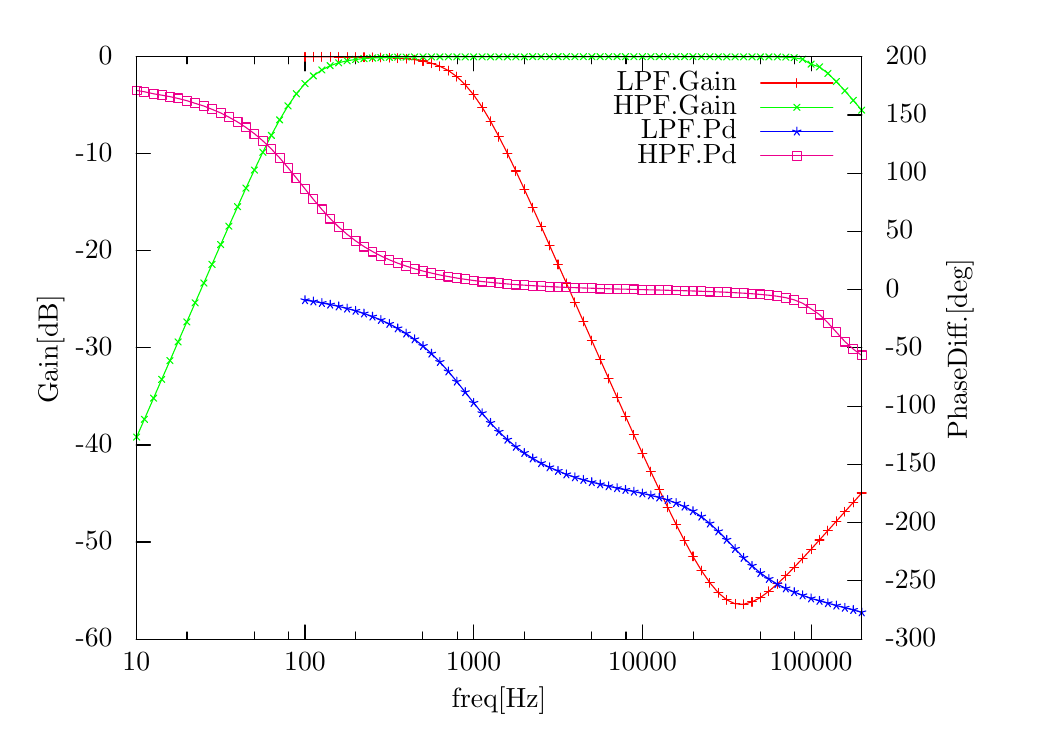
\begin{tikzpicture}[gnuplot]
%% generated with GNUPLOT 4.6p4 (Lua 5.1; terminal rev. 99, script rev. 100)
%% 2016年06月18日 10時34分17秒
\path (0.000,0.000) rectangle (12.500,8.750);
\gpcolor{color=gp lt color border}
\gpsetlinetype{gp lt border}
\gpsetlinewidth{1.00}
\draw[gp path] (1.320,0.985)--(1.500,0.985);
\node[gp node right] at (1.136,0.985) {-60};
\draw[gp path] (1.320,2.218)--(1.500,2.218);
\node[gp node right] at (1.136,2.218) {-50};
\draw[gp path] (1.320,3.450)--(1.500,3.450);
\node[gp node right] at (1.136,3.450) {-40};
\draw[gp path] (1.320,4.683)--(1.500,4.683);
\node[gp node right] at (1.136,4.683) {-30};
\draw[gp path] (1.320,5.916)--(1.500,5.916);
\node[gp node right] at (1.136,5.916) {-20};
\draw[gp path] (1.320,7.148)--(1.500,7.148);
\node[gp node right] at (1.136,7.148) {-10};
\draw[gp path] (1.320,8.381)--(1.500,8.381);
\node[gp node right] at (1.136,8.381) { 0};
\draw[gp path] (1.320,0.985)--(1.320,1.165);
\draw[gp path] (1.320,8.381)--(1.320,8.201);
\node[gp node center] at (1.320,0.677) { 10};
\draw[gp path] (1.965,0.985)--(1.965,1.075);
\draw[gp path] (1.965,8.381)--(1.965,8.291);
\draw[gp path] (2.818,0.985)--(2.818,1.075);
\draw[gp path] (2.818,8.381)--(2.818,8.291);
\draw[gp path] (3.255,0.985)--(3.255,1.075);
\draw[gp path] (3.255,8.381)--(3.255,8.291);
\draw[gp path] (3.463,0.985)--(3.463,1.165);
\draw[gp path] (3.463,8.381)--(3.463,8.201);
\node[gp node center] at (3.463,0.677) { 100};
\draw[gp path] (4.107,0.985)--(4.107,1.075);
\draw[gp path] (4.107,8.381)--(4.107,8.291);
\draw[gp path] (4.960,0.985)--(4.960,1.075);
\draw[gp path] (4.960,8.381)--(4.960,8.291);
\draw[gp path] (5.397,0.985)--(5.397,1.075);
\draw[gp path] (5.397,8.381)--(5.397,8.291);
\draw[gp path] (5.605,0.985)--(5.605,1.165);
\draw[gp path] (5.605,8.381)--(5.605,8.201);
\node[gp node center] at (5.605,0.677) { 1000};
\draw[gp path] (6.250,0.985)--(6.250,1.075);
\draw[gp path] (6.250,8.381)--(6.250,8.291);
\draw[gp path] (7.103,0.985)--(7.103,1.075);
\draw[gp path] (7.103,8.381)--(7.103,8.291);
\draw[gp path] (7.540,0.985)--(7.540,1.075);
\draw[gp path] (7.540,8.381)--(7.540,8.291);
\draw[gp path] (7.748,0.985)--(7.748,1.165);
\draw[gp path] (7.748,8.381)--(7.748,8.201);
\node[gp node center] at (7.748,0.677) { 10000};
\draw[gp path] (8.392,0.985)--(8.392,1.075);
\draw[gp path] (8.392,8.381)--(8.392,8.291);
\draw[gp path] (9.245,0.985)--(9.245,1.075);
\draw[gp path] (9.245,8.381)--(9.245,8.291);
\draw[gp path] (9.682,0.985)--(9.682,1.075);
\draw[gp path] (9.682,8.381)--(9.682,8.291);
\draw[gp path] (9.890,0.985)--(9.890,1.165);
\draw[gp path] (9.890,8.381)--(9.890,8.201);
\node[gp node center] at (9.890,0.677) { 100000};
\draw[gp path] (10.535,0.985)--(10.535,1.075);
\draw[gp path] (10.535,8.381)--(10.535,8.291);
\draw[gp path] (10.535,0.985)--(10.355,0.985);
\node[gp node left] at (10.719,0.985) {-300};
\draw[gp path] (10.535,1.725)--(10.355,1.725);
\node[gp node left] at (10.719,1.725) {-250};
\draw[gp path] (10.535,2.464)--(10.355,2.464);
\node[gp node left] at (10.719,2.464) {-200};
\draw[gp path] (10.535,3.204)--(10.355,3.204);
\node[gp node left] at (10.719,3.204) {-150};
\draw[gp path] (10.535,3.943)--(10.355,3.943);
\node[gp node left] at (10.719,3.943) {-100};
\draw[gp path] (10.535,4.683)--(10.355,4.683);
\node[gp node left] at (10.719,4.683) {-50};
\draw[gp path] (10.535,5.423)--(10.355,5.423);
\node[gp node left] at (10.719,5.423) { 0};
\draw[gp path] (10.535,6.162)--(10.355,6.162);
\node[gp node left] at (10.719,6.162) { 50};
\draw[gp path] (10.535,6.902)--(10.355,6.902);
\node[gp node left] at (10.719,6.902) { 100};
\draw[gp path] (10.535,7.641)--(10.355,7.641);
\node[gp node left] at (10.719,7.641) { 150};
\draw[gp path] (10.535,8.381)--(10.355,8.381);
\node[gp node left] at (10.719,8.381) { 200};
\draw[gp path] (1.320,8.381)--(1.320,0.985)--(10.535,0.985)--(10.535,8.381)--cycle;
\node[gp node center,rotate=-270] at (0.246,4.683) {Gain[dB]};
\node[gp node center,rotate=-270] at (11.792,4.683) {PhaseDiff.[deg]};
\node[gp node center] at (5.927,0.215) {freq[Hz]};
\node[gp node right] at (9.067,8.047) {LPF.Gain};
\gpcolor{color=gp lt color 0}
\gpsetlinetype{gp lt plot 0}
\draw[gp path] (9.251,8.047)--(10.167,8.047);
\draw[gp path] (3.463,8.379)--(3.569,8.379)--(3.677,8.379)--(3.783,8.379)--(3.891,8.378)%
  --(3.998,8.377)--(4.105,8.377)--(4.212,8.375)--(4.320,8.374)--(4.427,8.371)--(4.534,8.368)%
  --(4.641,8.363)--(4.748,8.355)--(4.855,8.343)--(4.962,8.326)--(5.069,8.299)--(5.176,8.260)%
  --(5.284,8.205)--(5.391,8.128)--(5.498,8.025)--(5.605,7.896)--(5.712,7.741)--(5.819,7.562)%
  --(5.926,7.364)--(6.034,7.152)--(6.141,6.929)--(6.248,6.699)--(6.355,6.464)--(6.462,6.225)%
  --(6.569,5.985)--(6.676,5.743)--(6.783,5.504)--(6.891,5.262)--(6.998,5.020)--(7.105,4.777)%
  --(7.212,4.535)--(7.319,4.294)--(7.426,4.054)--(7.533,3.814)--(7.640,3.578)--(7.748,3.343)%
  --(7.855,3.111)--(7.962,2.883)--(8.069,2.659)--(8.176,2.441)--(8.283,2.233)--(8.390,2.036)%
  --(8.497,1.856)--(8.605,1.700)--(8.712,1.573)--(8.819,1.483)--(8.926,1.433)--(9.033,1.428)%
  --(9.140,1.457)--(9.247,1.513)--(9.354,1.593)--(9.462,1.686)--(9.569,1.788)--(9.676,1.898)%
  --(9.783,2.010)--(9.890,2.126)--(9.997,2.244)--(10.104,2.363)--(10.211,2.482)--(10.319,2.602)%
  --(10.426,2.721)--(10.533,2.840);
\gpsetpointsize{4.00}
\gppoint{gp mark 1}{(3.463,8.379)}
\gppoint{gp mark 1}{(3.569,8.379)}
\gppoint{gp mark 1}{(3.677,8.379)}
\gppoint{gp mark 1}{(3.783,8.379)}
\gppoint{gp mark 1}{(3.891,8.378)}
\gppoint{gp mark 1}{(3.998,8.377)}
\gppoint{gp mark 1}{(4.105,8.377)}
\gppoint{gp mark 1}{(4.212,8.375)}
\gppoint{gp mark 1}{(4.320,8.374)}
\gppoint{gp mark 1}{(4.427,8.371)}
\gppoint{gp mark 1}{(4.534,8.368)}
\gppoint{gp mark 1}{(4.641,8.363)}
\gppoint{gp mark 1}{(4.748,8.355)}
\gppoint{gp mark 1}{(4.855,8.343)}
\gppoint{gp mark 1}{(4.962,8.326)}
\gppoint{gp mark 1}{(5.069,8.299)}
\gppoint{gp mark 1}{(5.176,8.260)}
\gppoint{gp mark 1}{(5.284,8.205)}
\gppoint{gp mark 1}{(5.391,8.128)}
\gppoint{gp mark 1}{(5.498,8.025)}
\gppoint{gp mark 1}{(5.605,7.896)}
\gppoint{gp mark 1}{(5.712,7.741)}
\gppoint{gp mark 1}{(5.819,7.562)}
\gppoint{gp mark 1}{(5.926,7.364)}
\gppoint{gp mark 1}{(6.034,7.152)}
\gppoint{gp mark 1}{(6.141,6.929)}
\gppoint{gp mark 1}{(6.248,6.699)}
\gppoint{gp mark 1}{(6.355,6.464)}
\gppoint{gp mark 1}{(6.462,6.225)}
\gppoint{gp mark 1}{(6.569,5.985)}
\gppoint{gp mark 1}{(6.676,5.743)}
\gppoint{gp mark 1}{(6.783,5.504)}
\gppoint{gp mark 1}{(6.891,5.262)}
\gppoint{gp mark 1}{(6.998,5.020)}
\gppoint{gp mark 1}{(7.105,4.777)}
\gppoint{gp mark 1}{(7.212,4.535)}
\gppoint{gp mark 1}{(7.319,4.294)}
\gppoint{gp mark 1}{(7.426,4.054)}
\gppoint{gp mark 1}{(7.533,3.814)}
\gppoint{gp mark 1}{(7.640,3.578)}
\gppoint{gp mark 1}{(7.748,3.343)}
\gppoint{gp mark 1}{(7.855,3.111)}
\gppoint{gp mark 1}{(7.962,2.883)}
\gppoint{gp mark 1}{(8.069,2.659)}
\gppoint{gp mark 1}{(8.176,2.441)}
\gppoint{gp mark 1}{(8.283,2.233)}
\gppoint{gp mark 1}{(8.390,2.036)}
\gppoint{gp mark 1}{(8.497,1.856)}
\gppoint{gp mark 1}{(8.605,1.700)}
\gppoint{gp mark 1}{(8.712,1.573)}
\gppoint{gp mark 1}{(8.819,1.483)}
\gppoint{gp mark 1}{(8.926,1.433)}
\gppoint{gp mark 1}{(9.033,1.428)}
\gppoint{gp mark 1}{(9.140,1.457)}
\gppoint{gp mark 1}{(9.247,1.513)}
\gppoint{gp mark 1}{(9.354,1.593)}
\gppoint{gp mark 1}{(9.462,1.686)}
\gppoint{gp mark 1}{(9.569,1.788)}
\gppoint{gp mark 1}{(9.676,1.898)}
\gppoint{gp mark 1}{(9.783,2.010)}
\gppoint{gp mark 1}{(9.890,2.126)}
\gppoint{gp mark 1}{(9.997,2.244)}
\gppoint{gp mark 1}{(10.104,2.363)}
\gppoint{gp mark 1}{(10.211,2.482)}
\gppoint{gp mark 1}{(10.319,2.602)}
\gppoint{gp mark 1}{(10.426,2.721)}
\gppoint{gp mark 1}{(10.533,2.840)}
\gppoint{gp mark 1}{(9.709,8.047)}
\gpcolor{color=gp lt color border}
\node[gp node right] at (9.067,7.739) {HPF.Gain};
\gpcolor{color=gp lt color 1}
\gpsetlinetype{gp lt plot 1}
\draw[gp path] (9.251,7.739)--(10.167,7.739);
\draw[gp path] (1.325,3.551)--(1.423,3.776)--(1.540,4.045)--(1.643,4.283)--(1.748,4.521)%
  --(1.851,4.759)--(1.962,5.013)--(2.068,5.256)--(2.178,5.507)--(2.282,5.744)--(2.392,5.995)%
  --(2.496,6.229)--(2.607,6.476)--(2.713,6.712)--(2.820,6.942)--(2.927,7.168)--(3.035,7.383)%
  --(3.141,7.579)--(3.247,7.757)--(3.354,7.911)--(3.463,8.039)--(3.569,8.138)--(3.677,8.213)%
  --(3.783,8.267)--(3.891,8.304)--(3.998,8.330)--(4.105,8.346)--(4.212,8.358)--(4.320,8.365)%
  --(4.427,8.370)--(4.534,8.373)--(4.641,8.375)--(4.748,8.377)--(4.855,8.378)--(4.962,8.379)%
  --(5.069,8.379)--(5.176,8.379)--(5.284,8.380)--(5.391,8.380)--(5.498,8.380)--(5.605,8.380)%
  --(5.712,8.380)--(5.819,8.380)--(5.926,8.380)--(6.034,8.380)--(6.141,8.380)--(6.248,8.380)%
  --(6.355,8.381)--(6.462,8.381)--(6.569,8.381)--(6.676,8.381)--(6.783,8.381)--(6.891,8.381)%
  --(6.998,8.381)--(7.105,8.381)--(7.212,8.381)--(7.319,8.381)--(7.426,8.381)--(7.533,8.381)%
  --(7.640,8.381)--(7.748,8.381)--(7.855,8.381)--(7.962,8.381)--(8.069,8.381)--(8.176,8.381)%
  --(8.283,8.381)--(8.390,8.381)--(8.497,8.381)--(8.605,8.381)--(8.712,8.380)--(8.819,8.380)%
  --(8.926,8.380)--(9.033,8.380)--(9.140,8.380)--(9.247,8.380)--(9.354,8.379)--(9.462,8.378)%
  --(9.569,8.376)--(9.676,8.369)--(9.783,8.349)--(9.890,8.286)--(9.997,8.252)--(10.104,8.169)%
  --(10.211,8.065)--(10.319,7.948)--(10.426,7.826)--(10.533,7.702);
\gppoint{gp mark 2}{(1.325,3.551)}
\gppoint{gp mark 2}{(1.423,3.776)}
\gppoint{gp mark 2}{(1.540,4.045)}
\gppoint{gp mark 2}{(1.643,4.283)}
\gppoint{gp mark 2}{(1.748,4.521)}
\gppoint{gp mark 2}{(1.851,4.759)}
\gppoint{gp mark 2}{(1.962,5.013)}
\gppoint{gp mark 2}{(2.068,5.256)}
\gppoint{gp mark 2}{(2.178,5.507)}
\gppoint{gp mark 2}{(2.282,5.744)}
\gppoint{gp mark 2}{(2.392,5.995)}
\gppoint{gp mark 2}{(2.496,6.229)}
\gppoint{gp mark 2}{(2.607,6.476)}
\gppoint{gp mark 2}{(2.713,6.712)}
\gppoint{gp mark 2}{(2.820,6.942)}
\gppoint{gp mark 2}{(2.927,7.168)}
\gppoint{gp mark 2}{(3.035,7.383)}
\gppoint{gp mark 2}{(3.141,7.579)}
\gppoint{gp mark 2}{(3.247,7.757)}
\gppoint{gp mark 2}{(3.354,7.911)}
\gppoint{gp mark 2}{(3.463,8.039)}
\gppoint{gp mark 2}{(3.569,8.138)}
\gppoint{gp mark 2}{(3.677,8.213)}
\gppoint{gp mark 2}{(3.783,8.267)}
\gppoint{gp mark 2}{(3.891,8.304)}
\gppoint{gp mark 2}{(3.998,8.330)}
\gppoint{gp mark 2}{(4.105,8.346)}
\gppoint{gp mark 2}{(4.212,8.358)}
\gppoint{gp mark 2}{(4.320,8.365)}
\gppoint{gp mark 2}{(4.427,8.370)}
\gppoint{gp mark 2}{(4.534,8.373)}
\gppoint{gp mark 2}{(4.641,8.375)}
\gppoint{gp mark 2}{(4.748,8.377)}
\gppoint{gp mark 2}{(4.855,8.378)}
\gppoint{gp mark 2}{(4.962,8.379)}
\gppoint{gp mark 2}{(5.069,8.379)}
\gppoint{gp mark 2}{(5.176,8.379)}
\gppoint{gp mark 2}{(5.284,8.380)}
\gppoint{gp mark 2}{(5.391,8.380)}
\gppoint{gp mark 2}{(5.498,8.380)}
\gppoint{gp mark 2}{(5.605,8.380)}
\gppoint{gp mark 2}{(5.712,8.380)}
\gppoint{gp mark 2}{(5.819,8.380)}
\gppoint{gp mark 2}{(5.926,8.380)}
\gppoint{gp mark 2}{(6.034,8.380)}
\gppoint{gp mark 2}{(6.141,8.380)}
\gppoint{gp mark 2}{(6.248,8.380)}
\gppoint{gp mark 2}{(6.355,8.381)}
\gppoint{gp mark 2}{(6.462,8.381)}
\gppoint{gp mark 2}{(6.569,8.381)}
\gppoint{gp mark 2}{(6.676,8.381)}
\gppoint{gp mark 2}{(6.783,8.381)}
\gppoint{gp mark 2}{(6.891,8.381)}
\gppoint{gp mark 2}{(6.998,8.381)}
\gppoint{gp mark 2}{(7.105,8.381)}
\gppoint{gp mark 2}{(7.212,8.381)}
\gppoint{gp mark 2}{(7.319,8.381)}
\gppoint{gp mark 2}{(7.426,8.381)}
\gppoint{gp mark 2}{(7.533,8.381)}
\gppoint{gp mark 2}{(7.640,8.381)}
\gppoint{gp mark 2}{(7.748,8.381)}
\gppoint{gp mark 2}{(7.855,8.381)}
\gppoint{gp mark 2}{(7.962,8.381)}
\gppoint{gp mark 2}{(8.069,8.381)}
\gppoint{gp mark 2}{(8.176,8.381)}
\gppoint{gp mark 2}{(8.283,8.381)}
\gppoint{gp mark 2}{(8.390,8.381)}
\gppoint{gp mark 2}{(8.497,8.381)}
\gppoint{gp mark 2}{(8.605,8.381)}
\gppoint{gp mark 2}{(8.712,8.380)}
\gppoint{gp mark 2}{(8.819,8.380)}
\gppoint{gp mark 2}{(8.926,8.380)}
\gppoint{gp mark 2}{(9.033,8.380)}
\gppoint{gp mark 2}{(9.140,8.380)}
\gppoint{gp mark 2}{(9.247,8.380)}
\gppoint{gp mark 2}{(9.354,8.379)}
\gppoint{gp mark 2}{(9.462,8.378)}
\gppoint{gp mark 2}{(9.569,8.376)}
\gppoint{gp mark 2}{(9.676,8.369)}
\gppoint{gp mark 2}{(9.783,8.349)}
\gppoint{gp mark 2}{(9.890,8.286)}
\gppoint{gp mark 2}{(9.997,8.252)}
\gppoint{gp mark 2}{(10.104,8.169)}
\gppoint{gp mark 2}{(10.211,8.065)}
\gppoint{gp mark 2}{(10.319,7.948)}
\gppoint{gp mark 2}{(10.426,7.826)}
\gppoint{gp mark 2}{(10.533,7.702)}
\gppoint{gp mark 2}{(9.709,7.739)}
\gpcolor{color=gp lt color border}
\node[gp node right] at (9.067,7.431) {LPF.Pd};
\gpcolor{color=gp lt color 2}
\gpsetlinetype{gp lt plot 2}
\draw[gp path] (9.251,7.431)--(10.167,7.431);
\draw[gp path] (3.463,5.289)--(3.569,5.273)--(3.677,5.254)--(3.783,5.233)--(3.891,5.210)%
  --(3.998,5.183)--(4.105,5.154)--(4.212,5.120)--(4.320,5.081)--(4.427,5.038)--(4.534,4.988)%
  --(4.641,4.931)--(4.748,4.866)--(4.855,4.792)--(4.962,4.707)--(5.069,4.611)--(5.176,4.504)%
  --(5.284,4.384)--(5.391,4.255)--(5.498,4.121)--(5.605,3.985)--(5.712,3.854)--(5.819,3.730)%
  --(5.926,3.618)--(6.034,3.517)--(6.141,3.427)--(6.248,3.349)--(6.355,3.280)--(6.462,3.220)%
  --(6.569,3.167)--(6.676,3.121)--(6.783,3.077)--(6.891,3.040)--(6.998,3.007)--(7.105,2.978)%
  --(7.212,2.951)--(7.319,2.926)--(7.426,2.902)--(7.533,2.880)--(7.640,2.858)--(7.748,2.835)%
  --(7.855,2.810)--(7.962,2.783)--(8.069,2.752)--(8.176,2.713)--(8.283,2.667)--(8.390,2.610)%
  --(8.497,2.541)--(8.605,2.453)--(8.712,2.354)--(8.819,2.246)--(8.926,2.131)--(9.033,2.017)%
  --(9.140,1.916)--(9.247,1.824)--(9.354,1.749)--(9.462,1.683)--(9.569,1.629)--(9.676,1.582)%
  --(9.783,1.541)--(9.890,1.502)--(9.997,1.471)--(10.104,1.441)--(10.211,1.411)--(10.319,1.383)%
  --(10.426,1.355)--(10.533,1.325);
\gppoint{gp mark 3}{(3.463,5.289)}
\gppoint{gp mark 3}{(3.569,5.273)}
\gppoint{gp mark 3}{(3.677,5.254)}
\gppoint{gp mark 3}{(3.783,5.233)}
\gppoint{gp mark 3}{(3.891,5.210)}
\gppoint{gp mark 3}{(3.998,5.183)}
\gppoint{gp mark 3}{(4.105,5.154)}
\gppoint{gp mark 3}{(4.212,5.120)}
\gppoint{gp mark 3}{(4.320,5.081)}
\gppoint{gp mark 3}{(4.427,5.038)}
\gppoint{gp mark 3}{(4.534,4.988)}
\gppoint{gp mark 3}{(4.641,4.931)}
\gppoint{gp mark 3}{(4.748,4.866)}
\gppoint{gp mark 3}{(4.855,4.792)}
\gppoint{gp mark 3}{(4.962,4.707)}
\gppoint{gp mark 3}{(5.069,4.611)}
\gppoint{gp mark 3}{(5.176,4.504)}
\gppoint{gp mark 3}{(5.284,4.384)}
\gppoint{gp mark 3}{(5.391,4.255)}
\gppoint{gp mark 3}{(5.498,4.121)}
\gppoint{gp mark 3}{(5.605,3.985)}
\gppoint{gp mark 3}{(5.712,3.854)}
\gppoint{gp mark 3}{(5.819,3.730)}
\gppoint{gp mark 3}{(5.926,3.618)}
\gppoint{gp mark 3}{(6.034,3.517)}
\gppoint{gp mark 3}{(6.141,3.427)}
\gppoint{gp mark 3}{(6.248,3.349)}
\gppoint{gp mark 3}{(6.355,3.280)}
\gppoint{gp mark 3}{(6.462,3.220)}
\gppoint{gp mark 3}{(6.569,3.167)}
\gppoint{gp mark 3}{(6.676,3.121)}
\gppoint{gp mark 3}{(6.783,3.077)}
\gppoint{gp mark 3}{(6.891,3.040)}
\gppoint{gp mark 3}{(6.998,3.007)}
\gppoint{gp mark 3}{(7.105,2.978)}
\gppoint{gp mark 3}{(7.212,2.951)}
\gppoint{gp mark 3}{(7.319,2.926)}
\gppoint{gp mark 3}{(7.426,2.902)}
\gppoint{gp mark 3}{(7.533,2.880)}
\gppoint{gp mark 3}{(7.640,2.858)}
\gppoint{gp mark 3}{(7.748,2.835)}
\gppoint{gp mark 3}{(7.855,2.810)}
\gppoint{gp mark 3}{(7.962,2.783)}
\gppoint{gp mark 3}{(8.069,2.752)}
\gppoint{gp mark 3}{(8.176,2.713)}
\gppoint{gp mark 3}{(8.283,2.667)}
\gppoint{gp mark 3}{(8.390,2.610)}
\gppoint{gp mark 3}{(8.497,2.541)}
\gppoint{gp mark 3}{(8.605,2.453)}
\gppoint{gp mark 3}{(8.712,2.354)}
\gppoint{gp mark 3}{(8.819,2.246)}
\gppoint{gp mark 3}{(8.926,2.131)}
\gppoint{gp mark 3}{(9.033,2.017)}
\gppoint{gp mark 3}{(9.140,1.916)}
\gppoint{gp mark 3}{(9.247,1.824)}
\gppoint{gp mark 3}{(9.354,1.749)}
\gppoint{gp mark 3}{(9.462,1.683)}
\gppoint{gp mark 3}{(9.569,1.629)}
\gppoint{gp mark 3}{(9.676,1.582)}
\gppoint{gp mark 3}{(9.783,1.541)}
\gppoint{gp mark 3}{(9.890,1.502)}
\gppoint{gp mark 3}{(9.997,1.471)}
\gppoint{gp mark 3}{(10.104,1.441)}
\gppoint{gp mark 3}{(10.211,1.411)}
\gppoint{gp mark 3}{(10.319,1.383)}
\gppoint{gp mark 3}{(10.426,1.355)}
\gppoint{gp mark 3}{(10.533,1.325)}
\gppoint{gp mark 3}{(9.709,7.431)}
\gpcolor{color=gp lt color border}
\node[gp node right] at (9.067,7.123) {HPF.Pd};
\gpcolor{color=gp lt color 3}
\gpsetlinetype{gp lt plot 3}
\draw[gp path] (9.251,7.123)--(10.167,7.123);
\draw[gp path] (1.325,7.952)--(1.423,7.936)--(1.540,7.910)--(1.643,7.893)--(1.748,7.874)%
  --(1.851,7.851)--(1.962,7.823)--(2.068,7.789)--(2.178,7.755)--(2.282,7.713)--(2.392,7.667)%
  --(2.496,7.614)--(2.607,7.552)--(2.713,7.483)--(2.820,7.404)--(2.927,7.313)--(3.035,7.210)%
  --(3.141,7.096)--(3.247,6.972)--(3.354,6.840)--(3.463,6.703)--(3.569,6.570)--(3.677,6.442)%
  --(3.783,6.326)--(3.891,6.219)--(3.998,6.125)--(4.105,6.043)--(4.212,5.970)--(4.320,5.907)%
  --(4.427,5.851)--(4.534,5.802)--(4.641,5.759)--(4.748,5.722)--(4.855,5.688)--(4.962,5.659)%
  --(5.069,5.633)--(5.176,5.609)--(5.284,5.589)--(5.391,5.570)--(5.498,5.554)--(5.605,5.539)%
  --(5.712,5.526)--(5.819,5.515)--(5.926,5.505)--(6.034,5.495)--(6.141,5.487)--(6.248,5.480)%
  --(6.355,5.473)--(6.462,5.467)--(6.569,5.461)--(6.676,5.456)--(6.783,5.452)--(6.891,5.448)%
  --(6.998,5.444)--(7.105,5.441)--(7.212,5.437)--(7.319,5.434)--(7.426,5.431)--(7.533,5.429)%
  --(7.640,5.426)--(7.748,5.423)--(7.855,5.420)--(7.962,5.418)--(8.069,5.415)--(8.176,5.412)%
  --(8.283,5.409)--(8.390,5.406)--(8.497,5.402)--(8.605,5.399)--(8.712,5.394)--(8.819,5.390)%
  --(8.926,5.384)--(9.033,5.378)--(9.140,5.371)--(9.247,5.362)--(9.354,5.352)--(9.462,5.339)%
  --(9.569,5.321)--(9.676,5.293)--(9.783,5.250)--(9.890,5.179)--(9.997,5.107)--(10.104,5.002)%
  --(10.211,4.883)--(10.319,4.764)--(10.426,4.668)--(10.533,4.587);
\gppoint{gp mark 4}{(1.325,7.952)}
\gppoint{gp mark 4}{(1.423,7.936)}
\gppoint{gp mark 4}{(1.540,7.910)}
\gppoint{gp mark 4}{(1.643,7.893)}
\gppoint{gp mark 4}{(1.748,7.874)}
\gppoint{gp mark 4}{(1.851,7.851)}
\gppoint{gp mark 4}{(1.962,7.823)}
\gppoint{gp mark 4}{(2.068,7.789)}
\gppoint{gp mark 4}{(2.178,7.755)}
\gppoint{gp mark 4}{(2.282,7.713)}
\gppoint{gp mark 4}{(2.392,7.667)}
\gppoint{gp mark 4}{(2.496,7.614)}
\gppoint{gp mark 4}{(2.607,7.552)}
\gppoint{gp mark 4}{(2.713,7.483)}
\gppoint{gp mark 4}{(2.820,7.404)}
\gppoint{gp mark 4}{(2.927,7.313)}
\gppoint{gp mark 4}{(3.035,7.210)}
\gppoint{gp mark 4}{(3.141,7.096)}
\gppoint{gp mark 4}{(3.247,6.972)}
\gppoint{gp mark 4}{(3.354,6.840)}
\gppoint{gp mark 4}{(3.463,6.703)}
\gppoint{gp mark 4}{(3.569,6.570)}
\gppoint{gp mark 4}{(3.677,6.442)}
\gppoint{gp mark 4}{(3.783,6.326)}
\gppoint{gp mark 4}{(3.891,6.219)}
\gppoint{gp mark 4}{(3.998,6.125)}
\gppoint{gp mark 4}{(4.105,6.043)}
\gppoint{gp mark 4}{(4.212,5.970)}
\gppoint{gp mark 4}{(4.320,5.907)}
\gppoint{gp mark 4}{(4.427,5.851)}
\gppoint{gp mark 4}{(4.534,5.802)}
\gppoint{gp mark 4}{(4.641,5.759)}
\gppoint{gp mark 4}{(4.748,5.722)}
\gppoint{gp mark 4}{(4.855,5.688)}
\gppoint{gp mark 4}{(4.962,5.659)}
\gppoint{gp mark 4}{(5.069,5.633)}
\gppoint{gp mark 4}{(5.176,5.609)}
\gppoint{gp mark 4}{(5.284,5.589)}
\gppoint{gp mark 4}{(5.391,5.570)}
\gppoint{gp mark 4}{(5.498,5.554)}
\gppoint{gp mark 4}{(5.605,5.539)}
\gppoint{gp mark 4}{(5.712,5.526)}
\gppoint{gp mark 4}{(5.819,5.515)}
\gppoint{gp mark 4}{(5.926,5.505)}
\gppoint{gp mark 4}{(6.034,5.495)}
\gppoint{gp mark 4}{(6.141,5.487)}
\gppoint{gp mark 4}{(6.248,5.480)}
\gppoint{gp mark 4}{(6.355,5.473)}
\gppoint{gp mark 4}{(6.462,5.467)}
\gppoint{gp mark 4}{(6.569,5.461)}
\gppoint{gp mark 4}{(6.676,5.456)}
\gppoint{gp mark 4}{(6.783,5.452)}
\gppoint{gp mark 4}{(6.891,5.448)}
\gppoint{gp mark 4}{(6.998,5.444)}
\gppoint{gp mark 4}{(7.105,5.441)}
\gppoint{gp mark 4}{(7.212,5.437)}
\gppoint{gp mark 4}{(7.319,5.434)}
\gppoint{gp mark 4}{(7.426,5.431)}
\gppoint{gp mark 4}{(7.533,5.429)}
\gppoint{gp mark 4}{(7.640,5.426)}
\gppoint{gp mark 4}{(7.748,5.423)}
\gppoint{gp mark 4}{(7.855,5.420)}
\gppoint{gp mark 4}{(7.962,5.418)}
\gppoint{gp mark 4}{(8.069,5.415)}
\gppoint{gp mark 4}{(8.176,5.412)}
\gppoint{gp mark 4}{(8.283,5.409)}
\gppoint{gp mark 4}{(8.390,5.406)}
\gppoint{gp mark 4}{(8.497,5.402)}
\gppoint{gp mark 4}{(8.605,5.399)}
\gppoint{gp mark 4}{(8.712,5.394)}
\gppoint{gp mark 4}{(8.819,5.390)}
\gppoint{gp mark 4}{(8.926,5.384)}
\gppoint{gp mark 4}{(9.033,5.378)}
\gppoint{gp mark 4}{(9.140,5.371)}
\gppoint{gp mark 4}{(9.247,5.362)}
\gppoint{gp mark 4}{(9.354,5.352)}
\gppoint{gp mark 4}{(9.462,5.339)}
\gppoint{gp mark 4}{(9.569,5.321)}
\gppoint{gp mark 4}{(9.676,5.293)}
\gppoint{gp mark 4}{(9.783,5.250)}
\gppoint{gp mark 4}{(9.890,5.179)}
\gppoint{gp mark 4}{(9.997,5.107)}
\gppoint{gp mark 4}{(10.104,5.002)}
\gppoint{gp mark 4}{(10.211,4.883)}
\gppoint{gp mark 4}{(10.319,4.764)}
\gppoint{gp mark 4}{(10.426,4.668)}
\gppoint{gp mark 4}{(10.533,4.587)}
\gppoint{gp mark 4}{(9.709,7.123)}
\gpcolor{color=gp lt color border}
\gpsetlinetype{gp lt border}
\draw[gp path] (1.320,8.381)--(1.320,0.985)--(10.535,0.985)--(10.535,8.381)--cycle;
%% coordinates of the plot area
\gpdefrectangularnode{gp plot 1}{\pgfpoint{1.320cm}{0.985cm}}{\pgfpoint{10.535cm}{8.381cm}}
\end{tikzpicture}

    \caption{発振直後の出力波形の周波数解析}
  \end{figure}

\begin{figure}[H]
    \begin{tabular}{cc}
      %---- 最初の図 ---------------------------
      \begin{minipage}[t]{0.5\hsize}
        \centering
        \includegraphics[width=7cm]{LPF_step.png}
        \caption{低域通過型フィルタのステップ応答}
      \end{minipage} &
      %---- 2番目の図 --------------------------
      \begin{minipage}[t]{0.5\hsize}
        \centering
        \includegraphics[width=7cm]{HPF_step.png}
        \caption{高域通過型フィルタのステップ応答}
      \end{minipage}
      %---- 図はここまで ----------------------
    \end{tabular}
  \end{figure}

減衰域での振幅特性の傾きはいずれもおおよそ-\SI{12}{\decibel}/octaveで、2次のフィルタとして妥当である。ステップ応答の結果も、立ち上がり・立ち下がりごとに一度だけオーバーシュートして(つまり、2回目の導関数=0の点で)入力に追いついている。

しかし、低域通過型フィルタの設計上の遮断周波数は\SI{1003}{\hertz}だが、測定結果では\SI{900}{\hertz}前後で、10\%の誤差がある。また、高域通過型フィルタの設計上の遮断周波数は\SI{100.3}{\hertz}だが、測定結果では少なくとも\SI{100}{\hertz}よりは小さく(おそらく、\SI{95}{\hertz}付近)、やはり数\%の誤差がある。しかし、これらは素子の値に数\%の誤差があれば容易に出現しうる(遮断周波数は$C$と$R$で決まるのであった。)から、ほとんど設計どおりであると評価できるだろう。

低域通過型フィルタの高周波領域では、少し減衰が見られるが、これはオペアンプの特性が強く表れたものである。一方、高域通過型フィルタの減衰域に見られる振幅特性の跳ね上がりの原因は不明だが、コンデンサの自己共振周波数を超えてしまい、等価直列インダクタンスによる効果が大きく表れてしまう領域に入った可能性が考えられる。

\section{参考資料}
\begin{enumerate}
\item 東京大学工学部 電子情報工学科・電気電子工学科(2016)『電気電子情報第一(前期)実験 テキスト』
\item R.M.Fano \& A.W.Lawson (1948) 菅原英彦訳(2009) 『マイクロ波フィルタの理論』丸善プラネット
\item 古賀利郎(1978)『伝送回路』コロナ社
\item 廣瀬明(2015) 『電気電子計測[第2版]』数理工学社

\end{enumerate}


\end{document}
